\documentclass[12pt]{amsbook}
%\usepackage[margin=1.5in]{geometry}
\usepackage[T1]{fontenc}
\usepackage{cmbright} 
\usepackage{todonotes}
\usepackage{amssymb,amsmath,amsthm,graphicx}
\usepackage{rotating}
\usepackage{setspace}
\usepackage{enumerate}
\usepackage{graphicx}
\usepackage{listings}
\usepackage{multirow}
\usepackage{color}
\usepackage{threeparttable}
\usepackage{caption}
\usepackage{subcaption}
\usepackage{hyperref}

\newtheorem{assump}{Assumption}[section]
\newtheorem{pro}{Proposition}[section]
\newtheorem{lem}{Lemma}[section]
\newtheorem{thm}{Theorem}[section]
\newtheorem{cor}{Corollary}[section]
\newtheorem{ineq}{Inequality}[section]
\newtheorem{defn}{Definition}[section]
\newtheorem{rem}{Remark}[section]
\newtheorem{ex}{Example}[section]
\theoremstyle{definition}
\newtheorem{alg}{Algorithm}[section]


\linespread{1.3}

\title{Lecture Notes for Part II of Econ 722}
\author{Francis J.\ DiTraglia}

\begin{document}
\maketitle

\tableofcontents

%!TEX root = ../main.tex
\chapter{``AIC-type'' Information Criteria}
You have probably know that Akaike's Information Criterion (AIC) summarizes the quality of a model by trading fit, measured by the maximized log likelihood, against complexity, measured by the number of estimated parameters.
But where does this complexity penalty come from?
In this chapter we'll take a closer look at the AIC and two closely criteria: Takeuichi's Information Criterion (TIC) and the ``corrected'' AIC (AIC$_c$) of Hurvich and Tsai (1989).
All three attempt to approximate the \textbf{Kullback-Leibler Divergence}, a fundamental quantity from information theory.
We'll set the stage by reviewing the main properties of the KL divergence and its connection to maximum likelihood estimation.


\section{The Kullback-Leibler Divergence}

\subsection{Basic Properties}
Suppose that $\mathbf{y}$ is a random vector drawn from a probability distribution $G$ with density $g(\mathbf{y})$. This is the \emph{true DGP} and is unknown to us. Since we don't know $g$, we attempt to approximate it using a parametric model $f(\mathbf{y}|\theta)$, where $\theta$ is a $p$-vector of parameters that we estimate via maximum likelihood.\footnote{I've written the model without covariates to keep the notation from getting out of control, but you could just as well write $f(\mathbf{y}|X,\theta)$. Similarly, I will sometimes write $f(\mathbf{y})$ for $f(\mathbf{y}|\theta)$ to simplify the notation below. } Since $f$ is not the true data density, a natural question is \emph{how well does $f$ approximate $g$}? It turns out that for maximum likelihood estimation there is a particularly convenient way to answer this question using the \textbf{Kullback Leibler Divergence}.


\begin{defn}[KL Divergence]
Let $E_G$ denote expectation with respect to the true, unknown data density $g$. Then the Kullback-Leibler divergence from $g$ to $f$ is given by
$$KL(g;f) = E_G \left[ \log{\left\{\frac{g(\textbf{y})}{f(\textbf{y})}\right\}}\right]= E_G\left[ \log{g(\textbf{y})}\right] - E_G\left[ \log{f(\textbf{y})} \right]$$
The quantity $E_G\left[ \log{f(\mathbf{y})} \right]$ is called the Expected Log-likelihood.
\end{defn}

\paragraph{Key Features of the KL Divergence}
There are several important features to note about the KL divergence:
\begin{enumerate}
\item It is \emph{not} symmetric: $KL(g;f)\neq KL(f;g)$. Hence, the KL divergence is \emph{not} a distance function (metric).
\item $KL(g;f) \geq 0$ with equality iff $f=g$. To see why, recall that, since $\log$ is a concave function, $-\log$ is convex. Thus
\begin{eqnarray*}
KL(g;f) &=& E_G \left[ \log{\left\{\frac{g(\mathbf{y})}{f(\mathbf{y})}\right\}}\right] = E_G \left[- \log{\left\{\frac{f(\mathbf{y})}{g(\mathbf{y})}\right\}}\right]\\\\
&\geq& -\log{\left\{E_G\left[ \frac{f(\mathbf{y})}{g(\mathbf{y})} \right]\right\}} = -\log{\left(\int g(\mathbf{y}) \frac{f(\mathbf{y})}{g(\mathbf{y})} \; d \mathbf{y} \right)}\\\\
&=& -\log{\left(\int f(\mathbf{y}) \;d \mathbf{y} \right)} = -\log{(1)} = 0
\end{eqnarray*}
by Jensen's Inequality. The inequality is strict only for a non-degenerate random variable and a strictly convex function. Since $-\log$ is strictly convex, the only way to make the inequality strict is for $f(\mathbf{y})/g(\mathbf{y})$ to be degenerate. This occurs precisely when $f=g$ almost everywhere.

\item Minimizing the KL divergence $KL(g;f)$ is \emph{equivalent} to maximizing the Expected Log-Likelihood $E_G[\log f(\mathbf{y})]$. This is because the first term in the KL divergence is a constant: it in no way depends on the model $f(\mathbf{y})$. The expected Log-likelihood enters negatively:
$$KL(g;f) = E_G\left[ \log{g(\textbf{y})}\right] - E_G\left[ \log{f(\textbf{y})} \right]$$
Thus, if we can find a way to estimate the Expected Log-likelihood, we can use the KL divergence for model selection: the larger the Expected Log-likelihood, the smaller the KL divergence, and the better the model.

\item The KL divergence equals the negative of \textbf{Boltzmann's Entropy} from Statistical Mechanics. Accordingly, it represents the \emph{information lost} when $g(\mathbf{y})$ is encoded by $f(\mathbf{y})$.
\end{enumerate}

\subsection{Relationship of MLE to KL}
It turns out that the KL divergence is inextricably linked to maximum likelihood estimation. To make the points a little clearer, I'll assume from now on that $\mathbf{y}$ consists of iid observations $Y_t$ for $t = 1, \hdots, T$. This is not in fact necessary for any of the derivations that follow, but it simplifies the notation. Since the expected log likelihood is unknown, we might try to approximate it using the sample analogue
$$E_{\widehat{G}}\left[\log{f(\textbf{y},\theta)} \right] = \frac{1}{T}\sum_{t=1}^T \log{f(Y_t, \theta)} = \frac{1}{T}\ell(\theta)$$
where we have replaced $G$ with the empirical distribution $\widehat{G}$. Now, by the Weak Law of Large Numbers for iid observations
$$\frac{1}{T} \ell(\theta) \overset{p}{\rightarrow} E_G\left[ \log{f(\textbf{y},\theta)} \right]$$
Under the standard regularity conditions (see Newey and McFadden, 1994) we can strengthen this result to show that
$$\hat{\theta} = \arg \max_{\theta \in \Theta} \frac{1}{T}\ell(\theta) \overset{p}{\rightarrow} \arg \max_{\theta \in \Theta} E_G\left[ \log{f(\textbf{y},\theta)}\right]$$
Since minimizing the KL divergence is the same as maximizing the expected log-likelihood we have the following result:
\begin{pro}
The ML estimator $\hat{\theta}$ converges in probability to the value of $\theta$ that minimizes the KL divergence from unknown true density $g(\mathbf{y})$ to the parametric family $f(\mathbf{y}|\theta)$. When $g(\mathbf{y})=f(\mathbf{y}|\theta)$ for some value of $\theta \in \Theta$, the divergence is minimized at zero.
\end{pro}


\subsection{A Na\"{i}ve Information Criterion}
If $g(\mathbf{y})$ were known, we could choose between two parametric models $f(\mathbf{y}|\theta)$ and $h(\mathbf{y}|\gamma)$ by comparing maximized Log-likelihoods. Define
\begin{eqnarray*}
\theta_0 &=& \arg \max_{\theta \in \Theta} E_G\left[ \log{f(\mathbf{y},\theta)} \right]\\
\gamma_0 &=& \arg \max_{\gamma\in \Gamma} E_G\left[ \log{h(\mathbf{y},\gamma)} \right]
\end{eqnarray*}
If $E_G\left[ \log{f(\mathbf{y},\theta_0)} \right] > E_G\left[ \log{h(\mathbf{y},\gamma_0)} \right]$, then the KL divergence from $g(\mathbf{y})$ to the parametric family $f_\theta$ is smaller than that from $g(\mathbf{y})$ to $h_\gamma$. Now, we know from above that $\hat{\theta} \overset{p}{\rightarrow} \theta_{0}$. Further, $\frac{1}{T}\ell(\theta) \overset{p}{\rightarrow} E_G\left[\log{f(\mathbf{y},\theta)} \right]$. Of course, $T$ will be constant across models, so why not use the maximized sample likelihood $\ell(\hat{\theta})$ for model comparison? Unfortunately, $\ell(\hat{\theta})$ is a \emph{biased estimator of the expected log likelihood} because is uses the data twice: first to estimate $\hat{\theta}$ and then directly in the sum $\sum_{t=1}^T \log{ f(Y_t,\hat{\theta})}$. Because $\hat{\theta}$ was chosen to conform to the idiosyncrasies of the data at hand, $\ell(\hat{\theta})$ is overly optimistic.

We can see this as follows. Since $\theta_0$ is the population minimizer of the KL divergence from $g$ to $f_\theta$, we have
\begin{eqnarray*}
KL\left[ g(\mathbf{y});f(\mathbf{y},\theta) \right] &\geq& KL\left[ g(\mathbf{y});f(\mathbf{y},\theta_0) \right]\\
E_G\left[ \log{g(\mathbf{y})}\right] - E_G\left[ \log{f(\mathbf{y},\theta)} \right] &\geq& E_G\left[ \log{g(\mathbf{y})}\right] - E_G\left[ \log{f(\mathbf{y},\theta_0)} \right]\\
E_G\left[ \log{f(\mathbf{y},\theta)} \right] &\leq& E_G\left[ \log{f(\mathbf{y},\theta_0)} \right]
\end{eqnarray*}
for all $\theta \in \Theta$. Recall that $\frac{1}{T}\ell(\theta) = E_{\widehat{G}}\left[ \log{f(\mathbf{y},\theta)}\right]$. By the definition of the maximum likelihood estimate, $\ell(\hat{\theta})\geq\ell(\theta_0)$. Thus,
$$E_{\widehat{G}}\left[ \log{f(\mathbf{y},\hat{\theta})}\right]\geq E_{\widehat{G}}\left[ \log{f\left(\mathbf{y},\theta_0\right)}\right] $$
In sample, the estimate $\hat{\theta}$ will show a higher maximized log-likelihood than the value of $\theta$ that maximizes the population log-likelihood. Thus, the sample analogue is \emph{overly optimistic}.

\section{The AIC and TIC}
In the previous section we saw that using the KL divergence to do model selection is equivalent to maximizing the expected log-likelihood across models. Unfortunately, using the maximized log-likelihood, based on the estimated parameters, is a biased estimator of this quantity: it is systematically too high. Both the AIC and the TIC address this problem by using asymptotic theory to get an approximate expression for the bias so that we can correct it.

To keep notation simple, throughout this section we'll assume that we have an iid sample of scalar random variables $Y_1, \hdots, Y_T$ drawn from a true but unknown distribution with density $g(y)$. As above we'll consider maximum likelihood estimation based on an approximating parametric density $f(y|\theta)$.

\subsection{Fundamental Expansion for MLE}
Under standard regularity conditions, see for example Newey and McFadden (1994), the maximum likelihood estimator $\widehat{\theta}$ can be expanded as
$$\widehat{\theta} = \theta_0 + J^{-1} \bar{U}_T + o_p(T^{-1/2})$$
where $\theta_0$ is value of $\theta$ that minimizes $KL$ divergence from $g$ to the parametric family of distributions $f(y|\theta)$ and
\begin{eqnarray*}
J &=& -E_G \left[ \frac{\partial^2 \log f(Y|\theta_0)}{\partial \theta \partial \theta'}\right]\\
\bar{U}_T &=& \frac{1}{T} \sum_{t=1}^T \frac{\partial \log f(Y_t|\theta_0)}{\partial\theta}
\end{eqnarray*}
Now, by the CLT, $\sqrt{T}\; \bar{U}_T \overset{d}{\rightarrow} U$ where $U\sim N_p(0, K)$ and
$$K = Var_G \left[ \frac{\partial \log f(Y|\theta_0)}{\partial\theta}\right] = E_G\left[ \frac{\partial \log f(Y|\theta_0)}{\partial\theta} \frac{\partial \log f(Y|\theta_0)}{\partial\theta'}\right]$$
Hence,
\begin{eqnarray*}
\sqrt{T}\left(\widehat{\theta} - \theta_0 \right) &=& \sqrt{T} \; J^{-1} \bar{U}_T + o_p(1) \\
&\overset{d}{\rightarrow}& J^{-1} U\\
&\sim& N_p(0, J^{-1}KJ^{-1})
\end{eqnarray*}
Note that when $g = f_\theta$ for some $\theta$, we have $K = J$ by the information matrix equality so the variance simplifies to $J^{-1}$.


\subsection{Estimating the Expected Log Likelihood}
To carry out model selection based on the KL divergence, we need to estimate the expected log likelihood. Under the iid assumption,
$$E_G[\log f(\mathbf{y}|\theta_0)] = E_G\left[\sum_{t=1}^T f(Y|\theta_0) \right] = T \; E_G[\log f(Y|\theta_0)]$$
so it is sufficient to work with the expected log likelihood of a single representative observation $Y$. Written as an integral,
$$E_G[\log f(Y|\theta_0)] = \int g(y) \log f(y|\theta_0) \; dy$$
There are two problems. First, we don't know $\theta_0$. Of course we do have an estimator $\widehat{\theta}$, so we might consider simply plugging it in to yield
$$\int g(y) \log f(y|\theta_0) \; dy \approx \int g(y) \log f(y|\widehat{\theta}) \; dy$$
Even with this approximation, however, we still don't know $g$, the true data density. As discussed above, trying to replace this integral with the sample analogue $\ell_T(\widehat{\theta})/T$, the maximized log-likelihood, introduces a bias. So what can we do? The idea behind the AIC and TIC is to \emph{estimate} this bias, which we'll write relative to the infeasible plug-in estimator. In other words:
$$Bias = \frac{\ell_T(\widehat{\theta})}{T} - \int g(y) \log f(y|\widehat{\theta}) dy$$
Now, as it turns out, we can expand the bias expression as follow:
\begin{eqnarray*}
Bias = \bar{Z}_T + (\widehat{\theta} - \theta_0)' J (\widehat{\theta} - \theta_0) + o_p(T^{-1})
\end{eqnarray*}
where
$$\bar{Z}_T = \frac{1}{T} \sum_{t=1}^T\left\{ \log f(Y_t|\theta_0) - E_G[\log f(Y|\theta_0)] \right\}$$
For a proof of this assertion, see Section \ref{sec:BiasExpansion}.

Now, recall that the bias expression depends on $\widehat{\theta}$ which is a random variable since it depends on the sample data. To address this, we will attempt to approximate the \emph{expectation} of the bias term, where, again, the expectation is taken over the sampling distribution of $\widehat{\theta}$. Using our asymptotic expansion:
$$E[Bias] \approx E[\bar{Z}_T] + E[(\widehat{\theta} - \theta_0)' J (\widehat{\theta} - \theta_0)]$$
Since $E[\bar{Z}_T] = 0$, this becomes
$$E[Bias] \approx E[(\widehat{\theta} - \theta_0)' J (\widehat{\theta} - \theta_0)]$$
Now, using the fundamental expansion for MLE from above
$$\sqrt{T}\left(\widehat{\theta} - \theta_0 \right) \overset{d}{\rightarrow} J^{-1}U$$
hence
$$T\left(\widehat{\theta} - \theta_0 \right)'J\left(\widehat{\theta} - \theta_0 \right) \overset{d}{\rightarrow} U' J^{-1} U$$
which suggests the approximation
$$E[Bias] \approx T^{-1} E[U'J^{-1}U]$$
Finally, using the almost magical properties of the trace operator, we have
\begin{eqnarray*}
E[U'J^{-1}U] &=& E\left[\mbox{trace} \left\{ U'J^{-1}U\right\} \right] = E\left[\mbox{trace} \left\{ J^{-1}UU'\right\} \right]\\
&=& \mbox{trace}\left\{ E[J^{-1}UU']\right\} = \mbox{trace}\left\{J^{-1} E[UU']\right\} \\
&=&\mbox{trace}\left\{ J^{-1} K\right\}
\end{eqnarray*}
Thus, we approximate the expected bias by $T^{-1}\mbox{trace}\left\{ J^{-1} K\right\}$. Finally, we correct the bias of the maximized log-likelihood and approximate the expected log likelihood by
$$E_G[\log f(Y|\theta_0)]\approx \frac{\ell(\widehat{\theta})}{T} - \frac{\mbox{trace}\left\{ J^{-1} K\right\}}{T}$$
multiplying through by $2T$ and substituting consistent estimators of the matrices $J$ and $K$ yields \textbf{Takeuchi's Information Criterion} (TIC)
$$TIC = 2\left[\ell(\widehat{\theta}) - \mbox{trace}\left\{ \widehat{J}^{-1} \widehat{K}\right\} \right]$$
The scaling is, of course, arbitrary but this particular choice is traditional. If there is a $\theta \in \Theta$ such that $g(y) = f(y|\theta)$ then the information matrix equality holds and $J^{-1} = K$. In this case $\mbox{trace}\left\{ J^{-1} K\right\} = \mbox{trace}\{\mathbf{I}_p\} = p$. Using this quantity as the bias correction yields \textbf{Akaike's Information Criterion}
$$AIC = 2 \left[\ell(\widehat{\theta}) - p \right]$$
Although the TIC and AIC are similar, there are several subtleties:
\begin{enumerate}
\item The bias correction for the AIC is derived under the assumption that the approximating model is \emph{correctly specified}, while the TIC is not.
  In this sense the AIC is a special case of the TIC.
\item It has been argued that for models where the Information Matrix Equality is not satisfied, the AIC will still be close to the TIC.
  (The log-likelihood term should dominate the bias correction in such situations.)
\item Typically, the matrices $K$ and $J$ are large, meaning that the estimates will have high variance (we need to estimate $p^2 + p$ elements). In contrast, the AIC a has much smaller variance because the bias correction \emph{does not depend on the data}. Thus, even if the model is mis-specified, it may be preferable to use AIC rather than TIC unless the sample size is large.
\end{enumerate}

\subsection{A Caveat}
To derive the TIC and AIC, we used the following expansion for the bias term
$$Bias = \bar{Z}_T + (\widehat{\theta} - \theta_0)' J (\widehat{\theta} - \theta_0) + o_p(T^{-1})$$
This holds under standard regularity conditions.
(For details on its derivation, see the next subsection.) However, we employed a bit of sleight of hand when we proceeded to approximate the expected bias using the mean of the limiting random variable $U'J^{-1}U$. For example, the expectation of ``truth'' relative to which the bias is calculated, namely
$$E_G\left[\int g(y) \log f(y|\widehat{\theta})\; dy\right]$$
does not exist in all cases. The bias correction remains reasonable in this case, as we see from the asymptotic expansion, but strictly speaking it doesn't make sense to talk about equating means.

\subsection{Appendix: Deriving the Bias Expansion}
\label{sec:BiasExpansion}
Consider a second order Taylor expansion around for $\log f(Y_t;\hat{\theta})$ around $\theta_0$:
\begin{align*}
\log f(Y_t;\hat{\theta}) &= \log f(Y_t;\theta_0)+\left.\frac{\partial\log f(Y_t;\theta)}{\partial\theta}\right|'_{\theta=\theta_0} (\widehat{\theta}-\theta_0) +  \\ 
& \quad + \frac{1}{2}(\widehat{\theta}-\theta_0)' \left.\frac{\partial^2\log f(Y_t;\theta)}{\partial\theta\partial\theta'}\right|_{\theta=\theta_0} (\widehat{\theta}-\theta_0) +R(Y_t;\hat{\theta}-\theta_0)
\end{align*}
where $R(Y_t;\hat{\theta}-\theta_0)$, the remainder, is such that:
\[
\left|R(Y_t;\widehat{\theta}-\theta_0)\right|\leq \frac{M(Y_t)}{(2+1)!}\| \widehat{\theta}-\theta_0 \|^{2+1}
\]
provided that all the derivatives of $\log f(Y_t;\theta)$ employed in the approximation are bounded above by $M(Y_t)$. The remainder has then the following property:
\[
\lim_{\widehat{\theta} \rightarrow \theta_0} \frac{R(Y_t;\widehat{\theta}-\theta_0)}{\| \widehat{\theta}-\theta_0 \|^{2}}=0\Rightarrow R(Y_t;\widehat{\theta}-\theta_0)=o(\| \widehat{\theta}-\theta_0 \|^{2})=o(1)\| \widehat{\theta}-\theta_0 \|^{2}
\]
Further implying that:
\[
R(Y_t;\hat{\theta}-\theta_0)=o_p(1)\| \hat{\theta}-\theta_0 \|^{2}=o_p(1)(\widehat{\theta}-\theta_0)'(\widehat{\theta}-\theta_0)
\]
Finally note that the $o_p(1)$ term may be a function of $Y_t$. Let's hence denote that term with $h(Y_t;\hat{\theta}-\theta_0)$ to take into account such possibility. Hence we can write:
\begin{align*}
\frac{\ell_{T}(\widehat{\theta})}{T}&= \frac{1}{T}\sum_{t=1}^{T}\left\{\log f(Y_t;\theta_0)+\left.\frac{\partial\log f(Y_t;\theta)}{\partial\theta}\right|'_{\theta=\theta_0}(\widehat{\theta}-\theta_0) + \right. \\ & \left. \quad +\frac{1}{2}(\widehat{\theta}-\theta_0)' \left.\frac{\partial^2\log f(Y_t;\theta)}{\partial\theta\partial\theta'}\right|_{\theta=\theta_0} (\widehat{\theta}-\theta_0) +h(Y_t;\hat{\theta}-\theta_0)(\widehat{\theta}-\theta_0)'(\widehat{\theta}-\theta_0) \right\}\\
& = \mathbb{E}_g \left[\log f(Y_t;\theta_0) \right]+\bar{Z}_T+\bar{U}'_T  (\widehat{\theta}-\theta_0)  - \frac{1}{2} (\widehat{\theta}-\theta_0)'  J_T  (\widehat{\theta}-\theta_0) \\
&\quad + \bar{h}(Y_t;\hat{\theta}-\theta_0)(\widehat{\theta}-\theta_0)'(\widehat{\theta}-\theta_0)
\end{align*}
with
\[
\bar{U}_T=\frac{1}{T}\sum_{t=1}^{T}\left.\frac{\partial\log f(Y_t;\theta)}{\partial\theta}\right|_{\theta=\theta_0}
\]
\[
J_T=-\frac{1}{T}\sum_{t=1}^{T}\left.\frac{\partial^2\log f(Y_t;\theta)}{\partial\theta\theta'}\right|_{\theta=\theta_0}
\] 
\[
\bar{h}(Y_t;\hat{\theta}-\theta_0)=\frac{1}{T}\sum_{t=1}^{T}h(Y_t;\hat{\theta}-\theta_0)
\]
Similarly we can write:
\begin{align*}
\int g(y)\log f(y;\widehat{\theta})dy & =  \int g(y)\left\{\log f(y;\theta_0)+\left.\frac{\partial\log f(y;\theta)}{\partial\theta}\right|'_{\theta=\theta_0}(\widehat{\theta}-\theta_0) + \right. \\ & \left. \quad +\frac{1}{2}(\widehat{\theta}-\theta_0)' \left.\frac{\partial^2\log f(y;\theta)}{\partial\theta\partial\theta'}\right|_{\theta=\theta_0} (\widehat{\theta}-\theta_0) + \right. \\
&\left. \quad+h(Y_t;\hat{\theta}-\theta_0)(\widehat{\theta}-\theta_0)'(\widehat{\theta}-\theta_0) \right\}dy \\
& = \mathbb{E}_g \left[\log f(Y_t;\theta_0) \right] - \frac{1}{2} (\widehat{\theta}-\theta_0)'  J  (\widehat{\theta}-\theta_0) + \\
& \quad + \mathbb{E}_g \left[ h(Y_t;\hat{\theta}-\theta_0) \right] (\widehat{\theta}-\theta_0)'(\widehat{\theta}-\theta_0)
\end{align*}
where the first order term drops since, by construction:
\[
\mathbb{E}_g \left[\left.\frac{\partial\log f(Y_t;\theta)}{\partial\theta}\right|_{\theta=\theta_0}\right]=0
\]
Now note that, fixing $\widehat{\theta}-\theta_0$, we have:
\[
\bar{h}(Y_t;\hat{\theta}-\theta_0) \longrightarrow_p \mathbb{E}_g \left[ h(Y_t;\hat{\theta}-\theta_0) \right] 
\]
and therefore:
\[
\bar{h}(Y_t;\hat{\theta}-\theta_0)=\mathbb{E}_g \left[ h(Y_t;\hat{\theta}-\theta_0) \right] +o_p(1)
\]
which gives us:
\begin{align*}
\bar{h}(Y_t;\hat{\theta}-\theta_0)(\widehat{\theta}-\theta_0)'(\widehat{\theta}-\theta_0)&= \mathbb{E}_g \left[ h(Y_t;\hat{\theta}-\theta_0) \right] (\widehat{\theta}-\theta_0)'  (\widehat{\theta}-\theta_0) + \\
& \quad +o_p\left(1\right)T^{-1}\sqrt{T} (\widehat{\theta}-\theta_0)' (\widehat{\theta}-\theta_0)\sqrt{T} \\
&= \mathbb{E}_g \left[ h(Y_t;\hat{\theta}-\theta_0) \right] (\widehat{\theta}-\theta_0)' (\widehat{\theta}-\theta_0) + \\
&\quad+o_p\left(1\right)T^{-1}O_p\left(1\right)^2\\
&= \mathbb{E}_g \left[ h(Y_t;\hat{\theta}-\theta_0) \right] (\widehat{\theta}-\theta_0)' (\widehat{\theta}-\theta_0) + \\
&\quad+o_p\left(T^{-1}\right)
\end{align*}
Further noting that:
\[
\text{p}\lim_{T\rightarrow\infty} J_T=J \Leftrightarrow J_T=J+o_p(1)
\]
which implies:
\begin{align*}
 (\widehat{\theta}-\theta_0)'  J_T  (\widehat{\theta}-\theta_0) &=  (\widehat{\theta}-\theta_0)'  J (\widehat{\theta}-\theta_0) +o_p\left(1\right)T^{-1}\sqrt{T}(\widehat{\theta}-\theta_0)'(\widehat{\theta}-\theta_0)\sqrt{T} \\
&= (\widehat{\theta}-\theta_0)'  J  (\widehat{\theta}-\theta_0) +o_p\left(1\right)T^{-1}O_p\left(1\right)^2\\
&= (\widehat{\theta}-\theta_0)'  J  (\widehat{\theta}-\theta_0) +o_p\left(T^{-1}\right)
\end{align*}
and recalling that:
\[
\bar{U}_T=J (\widehat{\theta}-\theta_0 )+o_p\left(T^{-1/2}\right)
\]
which similarly gives:
\begin{align*}
\bar{U}'_T (\widehat{\theta}-\theta_0)&=  (\widehat{\theta}-\theta_0)'  J  (\widehat{\theta}-\theta_0) +o_p\left(T^{-1/2}\right)T^{-1/2}\sqrt{T}(\widehat{\theta}-\theta_0) \\
&= (\widehat{\theta}-\theta_0)'  J (\widehat{\theta}-\theta_0) +o_p\left(T^{-1/2}\right)T^{-1/2}O_p\left(1\right)\\
&= (\widehat{\theta}-\theta_0)'  J  (\widehat{\theta}-\theta_0) +o_p\left(T^{-1}\right)
\end{align*}
we can finally write:
\begin{align*}
\frac{\ell_{T}(\widehat{\theta})}{T}-\int g(y)\log f(y;\widehat{\theta})dy &= \bar{Z}_T+\left(\widehat{\theta}-\theta_0\right)'  J \left(\widehat{\theta}-\theta_0\right)  + o_p\left(T^{-1}\right)
\end{align*}

\section{The Corrected AIC}
To derive the TIC and AIC we used asymptotic theory to construct an analytical bias correction. Such approximations tend to work as long as $T$ is fairly large relative to $p$ but when this is not the case, they can break down. 
We'll now consider an alternative that makes stronger assumptions and relies on \emph{exact} small-sample theory rather than asymptotics: the ``Corrected'' AIC, or AIC$_c$, of Hurvich and Tsai (1989).
Suppose that the true DGP is a linear regression model:
$$\textbf{y} = X\beta_0 + \boldsymbol{\epsilon}$$
where $\mathbf{\epsilon} \sim N(\mathbf{0}, \sigma_0^2 \mathbf{I}_T)$. 
Then $\mathbf{y}|X \sim N(X\beta_0, \sigma_0^2 \mathbf{I}_T)$ so the likelihood is
$$g(\textbf{y}|X;\beta_0, \sigma^2_0) = \left(2\pi\sigma_0^2\right)^{-T/2} \exp\left\{ -\frac{1}{2\sigma^2}(y - X\beta_0)'(y - X\beta_0)\right\}$$
and the log-likelihood is
$$\log\left[g(\textbf{y}|X;\beta_0, \sigma_0^2)\right] = -\frac{T}{2}\log(2\pi) -\frac{T}{2} \log(\sigma^2_0) - \frac{1}{2\sigma_0^2}\left(\textbf{y} - X\beta_0\right)'\left(\textbf{y} -X\beta_0\right)$$
Now suppose we evaluated the log-likelihood at some \emph{other} parameter values $\beta_1$ and $\sigma^2_1$. The vector $\beta_1$ might, for example, correspond to dropping some regressors from the model by setting their coefficients to zero, or perhaps adding in some additional regressors. 
We have
$$\log[f(\textbf{y}|X;\beta_1, \sigma_1^2)] = -\frac{T}{2}\log(2\pi) -\frac{T}{2} \log(\sigma^2_1) - \frac{1}{2\sigma_1^2}\left(\textbf{y} - X\beta_1\right)'\left(\textbf{y} -X\beta_1\right)$$
Since we've specified the density from which the data were generated as well as the density of the approximating model, we can \emph{directly calculate} the KL divergence rather than trying to find a reasonable large sample approximation. It turns out that for this example 
$$KL(g;f) = \frac{T}{2}\left[\frac{\sigma_0^2}{\sigma_1^2} - \log\left(\frac{\sigma_0^2}{\sigma_1^2}\right) - 1 \right] + \left(\frac{1}{2 \sigma_1^2}\right)\left(\beta_0 - \beta_1\right)'X'X\left(\beta_0 - \beta_1\right)$$ 
as shown in Section \ref{sec:KLderivation}.
We need to estimate this quantity for it to be of any use in model selection. If let $\widehat{\beta}$ and $\widehat{\sigma}^2$ be the maximum likelihood estimators of $\beta_1$ and $\sigma_1^2$ and substitute them into the expression for the KL divergence, we have
\begin{eqnarray*}
\widehat{KL}(g;f) &=& \frac{T}{2}\left[\frac{\sigma_0^2}{\widehat{\sigma}^2} - \log\left(\frac{\sigma_0^2}{\widehat{\sigma}^2} \right) - 1\right] + \left(\frac{1}{2\widehat{\sigma}^2} \right)\left(\beta_0 - \widehat{\beta}\right)X'X\left(\beta_0 - \widehat{\beta}\right)
\end{eqnarray*}
We still have two problems. First, we haven't been entirely clear about what $\beta_1$ and $\sigma_1$ are. At the moment, they seem to be something like ``pseudo-true'' values. Second, and more importantly, we don't know $\beta_0$ and $\sigma_0^2$ so we can't use the preceding expression to compare models.

Hurvich and Tsai (1989) address both of these problems with the assumption that all models under consideration are \emph{at least correctly specified}. That is, while they may include a regressor whose coefficient is in fact zero, they do not exclude any regressors with a non-zero coefficient. This is the same assumption that we used above to reduce TIC to AIC. Under this assumption, $\beta_1$ and $\sigma_1^2$ \emph{are precisely the same} as $\beta_0$ and $\sigma_0^2$. More importantly, we can use all of the standard results for the exact finite sample distribution of regression estimators to help us. The idea is to construct an \emph{unbiased} estimator of the KL divergence. Taking expecations and rearranging slightly, we have
\begin{eqnarray*}
E\left[\widehat{KL}(g;f) \right] &=&\frac{T}{2}\left\{ E\left[\frac{\sigma_0^2}{\widehat{\sigma}^2} \right] - \log(\sigma_0^2) + E\left[\log(\widehat{\sigma}^2)\right] -1 \right\}\\
&& \quad + \; \frac{1}{2}E\left[\left(\frac{1}{\widehat{\sigma}^2} \right)\left(\widehat{\beta}-\beta_0 \right)X'X\left(\widehat{\beta}-\beta_0\right) \right]
\end{eqnarray*}
Now, under our assumptions $T\widehat{\sigma}^2/\sigma_0^2 \sim \chi^2_{T-k}$ where $k$ is the number of estimated coefficients in $\widehat{\beta}$. Further, if $Z \sim \chi^2_\nu$ then $E[1/Z] = 1/(\nu-2)$. It follows that
$$E\left[\frac{\sigma_0^2}{\widehat{\sigma}^2} \right] = E\left[\frac{T}{T\widehat{\sigma}^2/\sigma_0^2} \right] = \frac{T}{T - k - 2}$$
We can rewrite the final term similarly:
$$E\left[\left(\frac{1}{\widehat{\sigma}^2} \right)\left(\widehat{\beta}-\beta_0 \right)X'X\left(\widehat{\beta}-\beta_0\right) \right] = E\left[\left(\frac{T}{T\widehat{\sigma}^2/\sigma_0^2} \right)\frac{\left(\widehat{\beta}-\beta_0 \right)X'X\left(\widehat{\beta}-\beta_0\right)}{\sigma_0^2} \right]$$
Under our assumptions the two terms in the product are independent, so we can break apart the expectation. First, we have
$$E\left[\frac{T}{T\widehat{\sigma}^2/\sigma_0^2} \right] = \frac{T}{T - k - 2}$$
as above. For the second part,
$$\frac{\left(\widehat{\beta}-\beta_0 \right)X'X\left(\widehat{\beta}-\beta_0\right)}{\sigma_0^2} \sim \chi^2_k$$
and hence
$$E\left[\frac{\left(\widehat{\beta}-\beta_0 \right)X'X\left(\widehat{\beta}-\beta_0\right)}{\sigma_0^2} \right] = k$$
Putting all the pieces together,
\begin{eqnarray*}
E\left[\widehat{KL}(g;f) \right] &=&\frac{T}{2}\left\{ E\left[\frac{\sigma_0^2}{\widehat{\sigma}^2} \right] + \log(\sigma_0^2) - E\left[\log(\widehat{\sigma}^2)\right] -1 \right\}\\
&& \quad + \; \frac{1}{2}E\left[\left(\frac{1}{\widehat{\sigma}^2} \right)\left(\widehat{\beta}-\beta_0 \right)X'X\left(\widehat{\beta}-\beta_0\right) \right]\\
&=& \frac{T}{2} \left( \frac{T}{T-k-2} - \log(\sigma_0^2) + E\left[\log(\widehat{\sigma}^2)\right] -1\right) + \frac{T}{2}\left(\frac{k}{T - k -2}\right)\\
&=& \frac{T}{2} \left(\frac{T + k}{T - k -2} - \log(\sigma_0^2) + E\left[\log(\widehat{\sigma}^2)\right] -1\right)
\end{eqnarray*}
Since $\log(\widehat{\sigma}^2)$ is an unbiased estimator of $E[\log(\widehat{\sigma}^2)]$, substituting this give us an unbiased estimator of $E\left[\widehat{KL}(g;f) \right]$ as desired.
The only terms that vary across candidate models are the first and the third. Moreover, the multiplicative factor of $T/2$ does not affect model selection. Hence, the criterion is
$$AIC_c = \log(\widehat{\sigma}^2) + \frac{T + k}{T - k -2}$$
In its broad strokes, this makes perfect sense. The residual error variance $\widehat{\sigma}^2$ measures in-sample fit. But since in-sample fit is a mis-leading guide to out-of-sample fit, we add a complexity penalty. Note that the way this expression is written, \emph{smaller} values indicate a better model. 

So how does this compare to the plain-vanilla AIC for normal linear regression? The maximum likelihood estimators for this problem are
\begin{eqnarray*}
\widehat{\beta} &=& (X'X)^{-1}X'\mathbf{y}\\
\widehat{\sigma}^2 &=& \frac{(\mathbf{y} - X\widehat{\beta})'(\mathbf{y} - X\widehat{\beta})}{T}
\end{eqnarray*}
It follows that the maximized log-likehood is
\begin{eqnarray*}
\log\left[f(\mathbf{y}|X;\widehat{\beta})\right] &=& -\frac{T}{2} \log(\widehat{\sigma}^2) - \frac{1}{2\widehat{\sigma}^2}(y - X\widehat{\beta})'(y -X\widehat{\beta})\\
&=& -\frac{T}{2} \log(\widehat{\sigma}^2) - \frac{T}{2}
\end{eqnarray*}
by substituting $T\widehat{\sigma}^2$ for the numerator of the second term. Hence, the AIC for this problem is
$$AIC = 2\left(\ell(\widehat{\beta}) - k \right) = -T\log(\widehat{\sigma}^2) - T - 2k $$
But this way of writing things uses the \emph{opposite} sign convention from AIC$_c$. It's important to keep track of this, since different authors use different sign conventions for information criteria. To make the AIC comparable with our scaling of the AIC$_c$, we multiply through by $-1/T$ yielding
$$AIC = \log(\widehat{\sigma}^2) + \frac{T + 2k}{T}$$
where \emph{smaller} values now indicate a better model.

\subsection{Appendix: Deriving the KL Divergence}
\label{sec:KLderivation}
  $$KL(g;f)= \int \log[g(\mathbf{y})] g(\mathbf{y}) \; d \mathbf{y} - \int \log[f(\mathbf{y})]g(\mathbf{y}) \; d \mathbf{y} = A - B$$
where
\begin{eqnarray*}
A &=&\int \left[-\frac{T}{2}\log(2\pi) -\frac{T}{2} \log(\sigma^2_0) - \frac{1}{2\sigma_0^2}\left(\textbf{y} - X\beta_0\right)'\left(\textbf{y} -X\beta_0\right) \right] g(\mathbf{y})\; d\mathbf{y}\\
&=& -\frac{T}{2}\left[ \log(2\pi) + \log(\sigma^2_0)\right] - \frac{1}{2\sigma_0^2} E_{\mathbf{y}|X}\left[\left(\textbf{y} - X\beta_0\right)'\left(\textbf{y} -X\beta_0\right)\right]\\
&=& -\frac{T}{2}\left[ \log(2\pi) + \log(\sigma^2_0)\right] - \frac{1}{2\sigma_0^2}\mbox{trace}\left\{ E_{\mathbf{y}|X}\left[\left(\textbf{y} - X\beta_0\right)\left(\textbf{y} -X\beta_0\right)'\right]\right\}\\
&=& -\frac{T}{2}\left[ \log(2\pi) + \log(\sigma^2_0)\right] - \frac{1}{2\sigma_0^2}\mbox{trace}\left\{ Var(\mathbf{y}|X)\right\}\\
&=& -\frac{T}{2}\left[ \log(2\pi) + \log(\sigma^2_0)\right] - \frac{1}{2\sigma_0^2}\left(T \sigma_0^2\right)\\
&=& -\frac{T}{2}\left[ \log(2\pi) + \log(\sigma^2_0) + 1 \right]
\end{eqnarray*}
and
\begin{eqnarray*}
B &=& \int \left[ -\frac{T}{2}\log(2\pi) -\frac{T}{2} \log(\sigma^2_1) - \frac{1}{2\sigma_1^2}\left(\textbf{y} - X\beta_1\right)'\left(\textbf{y} -X\beta_1\right) \right] g(\mathbf{y})\; d \mathbf{y}\\
&=& -\frac{T}{2}\left[\log(2\pi) + \log(\sigma^2_1) \right]- \frac{1}{2\sigma_1^2}E_{\mathbf{y}|X}\left[\left(\textbf{y} - X\beta_1\right)'\left(\textbf{y} -X\beta_1\right)\right]\\
&=& -\frac{T}{2}\left[\log(2\pi) + \log(\sigma^2_1) \right] - \left(\frac{1}{2\sigma_1^2}\right)C
\end{eqnarray*}
where we define $C$ as
\begin{eqnarray*}
C &=& E_{\mathbf{y}|X}\left[\left(\textbf{y} - X\beta_1\right)'\left(\textbf{y} -X\beta_1\right)\right]\\
&=&E_{\mathbf{y}|X}\left[\left\{ \left(\mathbf{y} - X\beta_0\right) + X\left(\beta_0 - \beta_1\right)\right\}'\left\{ \left(\mathbf{y} - X\beta_0\right)+ X\left(\beta_0 - \beta_1\right)\right\} \right]\\
&=& E_{\mathbf{y}|X}\left[\left(\mathbf{y} - X\beta_0\right)'\left(\mathbf{y} - X\beta_0\right)\right] +\; E_{\mathbf{y}|X}\left[\left(\mathbf{y} -X\beta_0\right)'X\left(\beta_0 - \beta_1\right)\right] \\
&& \quad +\; E_{\mathbf{y}|X}\left\{\left[X\left(\beta_0 -\beta_1 \right) \right]'\left(\mathbf{y} - X\beta_0 \right)\right\} + \;E_{\mathbf{y}|X}\left[\left\{X\left(\beta_0 - \beta_1\right)\right\}'\left\{X\left(\beta_0 - \beta_1\right)\right\} \right]\\
&=& Var(\mathbf{y}|X) + \; E_{\mathbf{y}|X}\left[\mathbf{y} - X\beta_0 \right]'X(\beta_0 -\beta_1) \\
&& \quad + \;(\beta_0 -\beta_1)'X'E_{\mathbf{y}|X}\left[\mathbf{y} - X\beta_0 \right] + \; (\beta_0 - \beta_1)X'X(\beta_0 - \beta_1)\\
&=& T\sigma_0^2 + 0 + 0 + (\beta_0 - \beta_1)X'X(\beta_0 - \beta_1)
\end{eqnarray*}
Hence,
\begin{eqnarray*}
B &=& -\frac{T}{2}\left[\log(2\pi) + \log(\sigma^2_1) \right] - \left(\frac{1}{2\sigma_1^2}\right) \left[ T\sigma_0^2 + (\beta_0 - \beta_1)X'X(\beta_0 - \beta_1)\right]\\
&=& -\frac{T}{2}\left[\log(2\pi) + \log(\sigma^2_1) + \frac{\sigma_0^2}{\sigma_1^2}\right] - \left(\frac{1}{2\sigma_1^2} \right)(\beta_0 - \beta_1)X'X(\beta_0 - \beta_1)
\end{eqnarray*}
and therefore,
\begin{eqnarray*}
KL(g;f) &=& A - B\\
&=& \left\{ -\frac{T}{2}\left[ \log(2\pi) + \log(\sigma^2_0) + 1 \right]\right\}\\
&& - \; \left\{ -\frac{T}{2}\left[\log(2\pi) + \log(\sigma^2_1) + \frac{\sigma_0^2}{\sigma_1^2}\right] - \left(\frac{1}{2\sigma_1^2} \right)(\beta_0 - \beta_1)X'X(\beta_0 - \beta_1) \right\}\\
&=& -\frac{T}{2} \left[ \log(\sigma_0^2) + 1 - \log(\sigma_1^2) - \frac{\sigma_0^2}{\sigma_1^2}\right] + \left(\frac{1}{2\sigma_1^2} \right)(\beta_0 - \beta_1)X'X(\beta_0 - \beta_1)\\
&=& \frac{T}{2}\left[\frac{\sigma_0^2}{\sigma_1^2} - \log\left(\frac{\sigma_0^2}{\sigma_1^2} \right) - 1\right] + \left(\frac{1}{2\sigma_1^2} \right)(\beta_0 - \beta_1)X'X(\beta_0 - \beta_1)
\end{eqnarray*}

%!TEX root = ../main.tex
\chapter{More on ``Classical'' Model Selection}


\section{Mallow's $C_p$}
Suppose that we want to predict $y$ from $\mathbf{x}$ using a linear regression model:
	$$\underset{(T\times1)}{\textbf{y}} = \underset{(T\times K)}{X} \underset{(K\times 1)}{\beta} + \boldsymbol{\epsilon}$$
Where $E[\boldsymbol{\epsilon}|X] = 0$ and $Var(\boldsymbol{\epsilon}|X) = \sigma^2 \mathbf{I}$. 
We know that the conditional mean is the minimum mean-squared error predictor.
This means that if $\beta$ were \emph{known}, we could never improve upon simply using all the regressors for prediction.
But since $\beta$ must be \emph{estimated} from the data, a bias-variance tradeoff arises.
In particular, we might be better off \emph{excluding} a regressor with small coefficient, since it adds very little predictive power but introduces additional estimation uncertainty.
Mallow's $C_p$ is a model selection criterion that trys to capture this idea by approximating the \emph{predictive mean squared error} of each model, relative to the infeasible optimum where $\beta$ is known.

We'll now consider using \emph{subsets} of $X$ rather than the full data matrix. 
Let $X_M$ denote a design matrix that possibly excludes some columns of $X$. 
The index $M$ refers to a particular \emph{model}. 
Accordingly, let $\widehat{\beta}_M$ be the least-squares estimator based on the design matrix $X_M$. 
We'll adopt the convention that $\widehat{\beta}_M$ is padded out with zeros for the elements of $\beta$ that are \emph{not estimated} under model $M$. 
This way we can write
	$$X\widehat{\beta}_M = X_{(-M)}\textbf{0} + X_M (X_M'X_M)^{-1} X_M'\textbf{y} = P_M \textbf{y}$$
Now, suppose we want to compare the predictive power of the competing estimators $\widehat{\beta}_M$ using mean-squared error. A na\"{i}ve idea would be to use in-sample prediction error to compare models:
	$$RSS(M) = (\textbf{y} - X\widehat{\beta}_M)'(\textbf{y} - X\widehat{\beta}_M)$$
As is well-known, however, the residual sum of squares can \emph{never} decrease even as we add irrelevant predictors to our model. In constrast, out-of-sample predictive ability can easily decrease when we add more predictors: there's a bias-variance tradeoff that arises from estimation uncertainty. Somehow or other we need to develop a criterion to take this into account.

We'll start off by calculating the predictive mean-squared error of $X\widehat{\beta}_M$ relative to the infeasible optimum, namely $X\beta$. Let $P_M = X_M(X_M'X_M)^{-1}X_M$. Then we have
\begin{eqnarray*}
	\left|\left|X\widehat{\beta}_M - X\beta\right|\right|^2 &=& (P_M \mathbf{y} - X\beta)'(P_M \mathbf{y} - X\beta)\\
		&=&\left\{P_M(Y-X\beta) - (\mathbf{I} - P_M)X\beta \right\}' \left\{P_M(Y-X\beta) - (\mathbf{I} - P_M)X\beta  \right\}\\
		&=&\left\{ P_M \boldsymbol{\epsilon} - (\mathbf{I}- P_M)X\beta\right\}'\left\{ P_M \boldsymbol{\epsilon} + (\mathbf{I}- P_M)X\beta \right\}\\
		&=&\boldsymbol{\epsilon}'P_M'P_M \boldsymbol{\epsilon} - \beta'X'(\mathbf{I}-P_M)'P_M\boldsymbol{\epsilon} \\
			&&\quad \quad - \;\boldsymbol{\epsilon}'P_M'(\mathbf{I} - P_M)X\beta + \beta'X' (\mathbf{I} - P_M)(\mathbf{I} - P_M)X\beta\\
		&=& \boldsymbol{\epsilon}'P_M \boldsymbol{\epsilon} + \beta'X'(\mathbf{I} - P_M)X\beta
\end{eqnarray*}
since $P_M$ and $(\mathbf{I} - P_M)$ are both symmetric and idempotent and their product in any order is zero. Thus, evaluating the predictive mean-squared error conditional on $X$, we have
	\begin{eqnarray*}
		\mbox{MSE}(M|X) &=& E\left[(X\widehat{\beta}_M - X\beta)'(X\widehat{\beta}_M - X\beta)|X \right]\\
		 &=& E\left[\boldsymbol{\epsilon}'P_M \boldsymbol{\epsilon}|X\right] + E\left[\beta'X'(\mathbf{I} - P_M)X\beta |X\right]\\
			&=&E\left[\mbox{trace}\left\{\boldsymbol{\epsilon}'P_M \boldsymbol{\epsilon}\right\}|X\right] + \beta'X'(\mathbf{I} - P_M)X\beta \\
		&=&\mbox{trace}\left\{E[\boldsymbol{\epsilon} \boldsymbol{\epsilon}'|X]P_M\right\} + \beta'X'(\mathbf{I} - P_M)X\beta \\
	&=&\mbox{trace}\left\{\sigma^2 P_M\right\} + \beta'X'(\mathbf{I} - P_M)X\beta \\
	&=& \sigma^2 k_M + \beta'X'(\mathbf{I} - P_M)X\beta
	\end{eqnarray*}
where $k_M$ denotes the number of regressors included in $X_M$ and we have used the fact that the trace of a projection matrix equals its dimension. 

So far, so good: we have derived an expression of the predictive mean-squared error of each model $M$. The problem is that it's infeasible: it depends on the unknown quantities $\sigma^2$ and $\beta$. To get around this, Mallow's $C_p$ constructs an \emph{unbiased} estimator of MSE. We proceed as follows. First, let $\widehat{\beta}$ be the estimator based on the full set of regressors, i.e.\ $\widehat{\beta} = (X'X)^{-1}X'\mathbf{y}$ and let $P_{X}$ be the corresponding projection matrix so that we have 
		$$X \widehat{\theta} = X(X'X)^{-1}X'\mathbf{y} = P_{X}\mathbf{y}$$
Using the fact that $P_MP_X = P_XP_M = P_M$, 
	\begin{eqnarray*}
		E\left[\widehat{\beta}'X'(\mathbf{I} - P_M)X\widehat{\beta} |X\right] &=& E\left[\mathbf{y}'P_X'(\mathbf{I} - P_M)P_{X}\mathbf{y} |X\right]\\
			&=& E\left[\mathbf{y}'(P_X'P_X - P_X'P_MP_X)\mathbf{y} |X\right]\\
			&=& E\left[\mathbf{y}'(P_X - P_M)\mathbf{y} |X\right]
	\end{eqnarray*}
which we can expand as
      \begin{eqnarray*}
     E\left[\mathbf{y}'(P_X - P_M)\mathbf{y} |X\right]&=& E\left[(X\beta + \boldsymbol{\epsilon})'(P_X - P_M)(X\beta + \boldsymbol{\epsilon})\mathbf{y} |X\right]\\
  		&=& E\left[\beta'X'(P_X - P_M)X\beta|X\right] + E[\boldsymbol{\epsilon}'(P_X - P_M)X\beta|X] \\
				&& \quad  + \; E[\beta'X'(P_X - P_M)\boldsymbol{\epsilon}|X] + E[\boldsymbol{\epsilon}'(P_X - P_M)\boldsymbol{\epsilon}|X]\\
			&=& \beta'X'(P_X - P_M)X\beta +  E[\boldsymbol{\epsilon}'(P_X - P_M)\boldsymbol{\epsilon}|X]
    \end{eqnarray*}
Now, we can re-write the first term as    
    \begin{eqnarray*}
    \beta'X'(P_X - P_M)X\beta  &=& \beta'X'P_X X\beta - \beta'X'P_MX\beta\\
      &=& \beta'X'X(X'X)^{-1}X' X\beta - \beta'X'P_MX\beta\\
      &=& \beta'X'X\beta - \beta'X'P_MX\beta\\
      &=& \beta'X'(\textbf{I} - P_M)X\beta
    \end{eqnarray*}
and evaluating the second term, we find that
    \begin{eqnarray*}
			E[\boldsymbol{\epsilon}'(P_X - P_M)\boldsymbol{\epsilon}|X]&=&E[\mbox{trace}\left\{\boldsymbol{\epsilon}'(P_X - P_M)\boldsymbol{\epsilon}\right\}|X]\\
      &=&  \mbox{trace}\left\{E[\boldsymbol{\boldsymbol{\epsilon}\epsilon}'|X](P_X - P_M)\right\}\\
			&=&\mbox{trace}\left\{\sigma^2(P_X - P_M)\right\}\\ 
			&=& \sigma^2 \left(\mbox{trace}\left\{P_X\right\} - \mbox{trace}\left\{P_M\right\}\right)\\ 
			&=& \sigma^2 (K - k_M) 
      \end{eqnarray*}
Hence, putting all the pieces together,
\begin{equation*}
E\left[\widehat{\beta}'X'(\mathbf{I} - P_M)X\widehat{\beta} |X\right] = \beta'X'(\mathbf{I}- P_M)X\beta +  \sigma^2 (K - k_M) 
\end{equation*}
In other words, substituting the estimator $\widehat{\beta}$ from the full model in order to estimate $\beta'X(\mathbf{I}- P_M)X\beta$ \emph{doesn't work}. 
The estimator $\widehat{\beta}'X'(\mathbf{I} - P_M)X\widehat{\beta}$ is \emph{biased upwards}.
However, we have an explicit expression for the bias, namely $\sigma^2 (K - k_M)$.
This means that if we can find an unbiased estimator of $\sigma^2$, we can \emph{correct} the bias in our estimator of $\beta'X(\mathbf{I}- P_M)X\beta$.
Fortunately there is an obvious unbiased estimator of $\sigma^2$: we simply use the residuals from the full model:
	$$\widehat{\sigma}^2 = \frac{\mathbf{y}'(\mathbf{I} - P_X)\mathbf{y}}{(T-K)}$$
Thus, 
	$$E[\widehat{\beta}'X'(\mathbf{I} - P_M)X\widehat{\beta} - \widehat{\sigma}^2(K- k_M) |X ] = \beta'X(\mathbf{I}- P_M)X\beta$$ 
Now we've managed to construct an unbiased estimator of the \emph{second} term of the MSE.
What about the first? This one is easy.
We already have an unbiased estimator of $\widehat{\sigma}^2$ and $k_M$ is a known constant: it's simply the number of regressors in model $M$.
Therefore, collecting terms
	\begin{eqnarray*}
		\mbox{MC}_M &=& \widehat{\sigma}^2 k_M + \left[\widehat{\beta}'X'(\mathbf{I} - P_M)X\widehat{\beta} - \widehat{\sigma}^2(K- k_M) \right]\\
			&=& \widehat{\beta}'X'(\mathbf{I} - P_M)X\widehat{\beta} + \widehat{\sigma}^2 (k_M - K)
	\end{eqnarray*}
is an unbiased estimator of $\mbox{MSE}(M|X)$. This criterion contains exactly the same information as Mallow's $C_p$ but expressed in a slightly different way. To get the formula from the textbooks, we need to do some more algebra. First, 
\begin{eqnarray*}
	MC_M - 2\widehat{\sigma}^2k_M &=& \widehat{\beta}'X'(\mathbf{I} - P_M)X\widehat{\beta} - K\widehat{\sigma}^2\\
	&=& \mathbf{y}'(P_X - P_M)\mathbf{y} -  K\widehat{\sigma}^2\\
   &=& \mathbf{y}'(P_X - P_M)\mathbf{y} - \left(\frac{K}{T-K}\right)\mathbf{y}'\left(\mathbf{I} - P_X\right)\mathbf{y}\\
		&=& \left(\frac{T-K}{T-K}\right)(\mathbf{y}'P_X\mathbf{y} - \mathbf{y}'P_M\mathbf{y}) - \left(\frac{K}{T-K}\right)(\mathbf{y}'\mathbf{y}' - \mathbf{y}'P_X \mathbf{y})\\
			&=&\left(\frac{T}{T-K}\right)\mathbf{y}'P_X \mathbf{y} - \mathbf{y}'P_M\mathbf{y} - \left(\frac{K}{T-K} \right)\mathbf{y}'\mathbf{y}  \\
			&=& \left(\frac{T}{T-K}\right)\mathbf{y}'P_X \mathbf{y} - \mathbf{y}'P_M\mathbf{y} + \left(\frac{T - K - T}{T-K} \right)\mathbf{y}'\mathbf{y}  \\
			&=&  \left(\frac{T}{T-K} \right)\mathbf{y}'P_X \mathbf{y} - \mathbf{y}' P_M \mathbf{y} + \left(1 - \frac{T}{T-K}\right)\mathbf{y}'\mathbf{y} \\
			&=&  \left(\frac{T}{T-K} \right)\mathbf{y}'P_X \mathbf{y} - \mathbf{y}' P_M \mathbf{y} + \mathbf{y}'\mathbf{y} - \left(\frac{T}{T-K}\right)\mathbf{y}'\mathbf{y}  \\
			&=& \mathbf{y}'\mathbf{y} - \mathbf{y}'P_M\mathbf{y} - \left(\frac{T}{T-K} \right)(\mathbf{y}'\mathbf{y} - \mathbf{y}'P_m\mathbf{y})\\
			&=& \mathbf{y}'(\mathbf{I} - P_M)\mathbf{y} - \left(\frac{T}{T-K}\right)\mathbf{y}'\left(\mathbf{I} - P_X\right)\mathbf{y}\\
			&=& \mathbf{y}'(\mathbf{I} - P_M)\mathbf{y} - T\widehat{\sigma}^2\\
			&=& RSS(M) - T\widehat{\sigma}^2
      \end{eqnarray*}
Substituting this into the expression for $\mbox{MC}_M$ we see that 
	$$\mbox{MC}_M = RSS(M) + \widehat{\sigma}^2(2 k_M - T)$$
which is much easier to interpret than the formula we had before.
Finally, dividing through by $\widehat{\sigma}^2$ gives Mallow's $C_p$
	$$C_p(M) = \frac{RSS(M)}{\widehat{\sigma}^2} + 2k_M - T$$
This expression tells us how we need to \emph{adjust} the residual sum of squares to account for the fact that in-sample fit is a misleading guide to out-of-sample predictive performance.

\section{Bayesian Information Criterion}
As in our derivation of TIC and AIC, we'll consider a setting with an iid sample of scalar random variables $Y_1, \hdots, Y_T$. The results still hold in the more general case, but this simplifies the notation. 

\subsection{Overview of the BIC}
Despite its name, the BIC is \emph{not} a Bayesian procedure. It is a large-sample Frequentist \emph{approximation} to Bayesian model selection:
	\begin{enumerate}
		\item Begin with a uniform prior on the set of candidate models so that it suffices to maximize the Marginal Likelihood.
		\item The BIC is a large sample approximation to the Marginal Likelihood:
		$$\int \pi(\beta_i)f_i(\mathbf{y}|\beta_i)d\beta_i$$
		where $i$ indexes models $M_i$ in a set $\mathcal{M}$.
		\item As usual when Bayesian procedures are subjected to Frequentist asymptotics, the priors on parameters vanish in the limit.
		\item We proceed by a \emph{Laplace Approximation} to the Marginal Likelihood
	\end{enumerate}

\subsection{Laplace Approximation}
For the moment simplify the notation by suppressing dependence on $M_i$. We want to approximate: 
	$$\int \pi(\beta)f(\mathbf{y}|\beta)d\beta$$
This is actually a common problem in applications of Bayesian inference:
	\begin{itemize} 
		\item Notice that $\pi(\beta)f(\mathbf{y}|\beta)$ is the \emph{kernel} of some probability density, i.e.\ the density without its normalizing constant. 
		\item \emph{How do we know this?} By Bayes' Rule 
	$$\pi(\beta|\mathbf{y}) = \frac{\pi(\beta)f(\mathbf{y}|\beta)}{\int \pi(\beta)f(\mathbf{y}|\beta) d\beta }$$
is a proper probability density and the denominator is \emph{constant} with respect to $\beta$. (The parameter has been ``integrated out.'')
	\item In Bayesian inference, we specify $\pi(\beta)$ and $f(\mathbf{y}|\beta)$, so $\pi(\beta)f(\mathbf{y}|\beta)$ is known. But to calculate the posterior we need to \emph{integrate} to find the normalizing constant.
	\item Only in special cases (e.g.\ conjugate families) can we find the exact normalizing constant. Typically some kind of approximation is needed:  
		\begin{itemize}
			\item Importance Sampling
			\item Markov-Chain Monte Carlo (MCMC)
			\item \emph{Laplace Approximation}
		\end{itemize}
	\end{itemize}
The Laplace Approximation is an \emph{analytical approximation} based on Taylor Expansion arguments. In Bayesian applications, the expansion is carried out around the posterior mode, i.e.\ the mode of $\pi(\beta)f(\mathbf{y}|\beta)$, but we will expand around the Maximum likelihood estimator. 

\begin{pro}[Laplace Approximation]
	\label{pro:laplace}
$$\int \pi(\beta)f(\mathbf{y}|\beta)d\beta \approx \frac{\exp\left\{ \ell(\hat{\beta}) \right\} \pi(\hat{\beta})(2\pi)^{p/2}}{n^{p/2}\left| J(\hat{\beta}) \right|^{1/2}}$$
	Where $\hat{\beta}$ is the \emph{maximum likelihood estimator}, $p$ the dimension of $\beta$ and
		$$J(\hat{\beta}) = -\frac{1}{n} \frac{\partial^2 \log f(\mathbf{y}|\hat{\beta})}{\partial \beta \partial \beta'}$$
\end{pro}

\begin{proof}
A rigorous proof of this result is complicated. The following is a sketch. First write $\ell(\beta)$ for $\log{f(\mathbf{y}|\beta)}$ so that 
$$\pi(\beta)f(\mathbf{y}|\beta) = \pi(\beta) \exp{\left\{ \log{f(\mathbf{y}| \beta)} \right\}}=\pi(\beta) \exp{\left\{ \log{\ell(\beta)} \right\}}$$
By a second-order Taylor Expansion around the MLE $\hat{\beta}$
	\begin{equation}
	\label{taylorell}
		\ell(\beta) = \ell(\hat{\beta}) +\frac{1}{2} \left( \beta - \hat{\beta}  \right)' \frac{\partial^2 \ell(\hat{\beta})}{\partial \beta \partial \beta'} \left( \beta - \hat{\beta}  \right) + R_\ell
	\end{equation}
since the derivative of $\ell(\beta)$ is zero at $\hat{\beta}$ by the definition of MLE. A first-order expansion is sufficient for $\pi(\beta)$ because the derivative does not vanish at $\hat{\beta}$
	\begin{equation}
		\label{taylorpi}
		\pi(\beta) = \pi(\hat{\beta}) +  \frac{\partial \pi(\hat{\beta})}{\partial \beta'} \left(\beta - \hat{\beta}  \right)+ R_\pi
	\end{equation}
Substituting Equations \ref{taylorell} and \ref{taylorpi},
	\begin{eqnarray*}
		\int \pi(\beta)f(\mathbf{y}|\beta)d\beta &=& \int \exp\left\{ \ell(\hat{\beta}) +\frac{1}{2} \left( \beta - \hat{\beta}  \right)' \frac{\partial^2 \ell(\hat{\beta})}{\partial \beta \partial \beta'} \left( \beta - \hat{\beta}  \right) + R_\ell \right\}\\
		&&\;\;\;\;\;\;\times \left[ \pi(\hat{\beta}) + \left(\beta - \hat{\beta}  \right)' \frac{\partial \pi(\hat{\beta})}{\partial \beta} + R_\pi \right]  d\beta\\\\
		&=& \exp\left\{ \ell(\hat{\beta}) \right\} (I_1 + I_2 + I_3)
	\end{eqnarray*}
where
	\begin{eqnarray*}
		I_1 &=& \pi(\hat{\beta}) \int  \exp{\left\{ \frac{1}{2} \left( \beta - \hat{\beta}  \right)' \frac{\partial^2 \ell(\hat{\beta})}{\partial \beta \partial \beta'} \left( \beta - \hat{\beta}  \right) + R_\ell\right\}} d\beta\\
		I_2 &=& \frac{\partial \pi(\hat{\beta})}{\partial \beta'}   \int  \left(\beta - \hat{\beta}  \right) \exp{\left\{ \frac{1}{2} \left( \beta - \hat{\beta}  \right)' \frac{\partial^2 \ell(\hat{\beta})}{\partial \beta \partial \beta'} \left( \beta - \hat{\beta}  \right) + R_\ell\right\}} d\beta\\
\\
		I_3 &=& \int R_\pi \; \exp{\left\{ \frac{1}{2} \left( \beta - \hat{\beta}  \right)' \frac{\partial^2 \ell(\hat{\beta})}{\partial \beta \partial \beta'} \left( \beta - \hat{\beta}  \right) + R_\ell\right\}} d\beta
	\end{eqnarray*}
Under certain regularity conditions (not the standard ones!) we can treat $R_\ell$ and $R_\pi$ as approximately equal to zero for large $n$ uniformly in $\beta$, so that
	\begin{eqnarray*}
		I_1 &\approx& \pi(\hat{\beta}) \int  \exp{\left\{ \frac{1}{2} \left( \beta - \hat{\beta}  \right)' \frac{\partial^2 \ell(\hat{\beta})}{\partial \beta \partial \beta'} \left( \beta - \hat{\beta}  \right) \right\}} d\beta\\
		I_2 &\approx& \frac{\partial \pi(\hat{\beta})}{\partial \beta'}   \int  \left(\beta - \hat{\beta}  \right) \exp{\left\{ \frac{1}{2} \left( \beta - \hat{\beta}  \right)' \frac{\partial^2 \ell(\hat{\beta})}{\partial \beta \partial \beta'} \left( \beta - \hat{\beta}  \right) \right\}} d\beta\\
		I_3 &\approx& 0
	\end{eqnarray*}	
Because $\hat{\beta}$ is the MLE, 
	$$\frac{\partial^2 \ell(\hat{\beta})}{\partial \beta \partial \beta'}$$ 
must be negative definite, so 
	$$-\frac{\partial^2 \ell(\hat{\beta})}{\partial \beta \partial \beta'}$$
is positive definite. It follows that 
	$$ \exp{\left\{ \frac{1}{2} \left( \beta - \hat{\beta}  \right)' \frac{\partial^2 \ell(\hat{\beta})}{\partial \beta \partial \beta'} \left( \beta - \hat{\beta}  \right) \right\}} =  \exp{\left\{ -\frac{1}{2} \left( \beta - \hat{\beta}  \right)'\left[ \left(-\frac{\partial^2 \ell(\hat{\beta})}{\partial \beta \partial \beta'}\right)^{-1} \right]^{-1}\left( \beta - \hat{\beta}  \right) \right\}}$$
can be viewed as the kernel of a Normal distribution with mean $\hat{\beta}$ and variance matrix 
	$$\left(-\frac{\partial^2 \ell(\hat{\beta})}{\partial \beta \partial \beta'}\right)^{-1}$$
Thus,
	$$\int  \exp{\left\{ \frac{1}{2} \left( \beta - \hat{\beta}  \right)' \frac{\partial^2 \ell(\hat{\beta})}{\partial \beta \partial \beta'} \left( \beta - \hat{\beta}  \right) \right\}} d\beta = \left(2\pi\right)^{p/2}\left| \left(-\frac{\partial^2 \ell(\hat{\beta})}{\partial \beta \partial \beta'}\right)^{-1} \right|^{1/2}$$
and
	$$\int \left(\beta - \hat{\beta}  \right)  \exp{\left\{ \frac{1}{2} \left( \beta - \hat{\beta}  \right)' \frac{\partial^2 \ell(\hat{\beta})}{\partial \beta \partial \beta'} \left( \beta - \hat{\beta}  \right) \right\}} d\beta = 0$$
Therefore,
	\begin{eqnarray*}
		\int \pi(\beta)f(\mathbf{y}|\beta)d\beta &\approx& \exp\left\{ \ell(\hat{\beta}) \right\}\pi(\hat{\beta}) \left(2\pi\right)^{p/2}\left| \left(-\frac{\partial^2 \ell(\hat{\beta})}{\partial \beta \partial \beta'}\right)^{-1} \right|^{1/2}\\
		&=&  \exp\left\{ \ell(\hat{\beta}) \right\}\pi(\hat{\beta}) \left(2\pi\right)^{p/2}\left|n \left(-\frac{1}{n}\frac{\partial^2 \ell(\hat{\beta})}{\partial \beta \partial \beta'}\right) \right|^{-1/2}\\\\
		&=&\frac{ \exp\left\{ \ell(\hat{\beta}) \right\}\pi(\hat{\beta}) \left(2\pi\right)^{p/2}}{n^{p/2}\left| J(\hat{\beta}) \right|^{1/2}}
	\end{eqnarray*}
\end{proof}


\subsection{Finally the BIC}
Now we re-introduce the dependence on the model $M_i$. Taking logs of the Laplace Approximation and multiplying by two (again, this is traditional but has no effect on model comparisons)
	\begin{eqnarray*}
		2 \log f(y|M_i) &=& 2 \log \left\{ \int f_i(y|\beta_i)\pi(\beta_i)d\beta_i \right\}\\
		&\approx& 2\ell(\hat{\beta}_i) -p\log(n) + p \log(2\pi)- \pi(\hat{\beta}_i)-\log \left| J(\hat{\beta_i}) \right|
	\end{eqnarray*}
The first two terms are $O_p(n)$ and $O_p(\log{n})$, while the last three are $O_p(1)$, hence negligible as $n\rightarrow \infty$. This gives us Schwarz's BIC
	$$BIC(M_i) = 2\log{f_i(\mathbf{y}|\hat{\beta}_i)} - p\log{n}$$
We choose the model $M_i$ for which $BIC(M_i)$ is largest. Notice that the prior on the parameter, $\pi(\beta)$, drops out in the limit, and recall that we began by putting a uniform prior on the \emph{models} under consideration. 

\section{Some Time Series Examples}
Thus far we've looked at a number of model selection criteria. 
Some of them, namely AIC, BIC and TIC, are completely portable: they can be applied to \emph{any} model that is estimated by maximum likelihood. 
Each of these can be immediately applied to time series data: if you have a routine to carry out ML estimation, be it conditional ML or the Kalman filter, it already produces all the quantities you need. 
In contrast, some of the other examples we considered, namely Mallow's $C_p$ and AIC$_c$, were derived for the special case of linear regression. 
How can we adapt these examples to time series data? Fortunately, if we're willing to use conditional ML estimation, some of the most widely used time series models \emph{are in fact} regression models. In this section we'll take a closer look at model selection for autoregression and vector autoregression models.


\subsection{Autoregressive Models}
For simplicity assume there is no constant term. Then the AR($p$) model is
	$$y_t = \phi_1 y_{t-1} + \phi_2 y_{t-2} + \cdots + \phi_p y_{t-p} + \epsilon_t$$
where $\epsilon_t \sim \mbox{iid} \; N(0,\sigma^2)$ and we observe a sample $y_1, \hdots, y_N$. We'll use conditional maximum likelihood, so we lose the first $p$ observations. Thus the \emph{effective sample size} is $T = N-p$. The conditional ML estimator of $\boldsymbol{\phi} = \left(\phi_1, \hdots, \phi_p \right)'$ is simply the least-squares estimator
	$$\widehat{\boldsymbol{\phi}} = (X'X)^{-1}X'\textbf{y}$$
where $\mathbf{y} = (y_{p+1}, y_{p+2}, \hdots, y_N)'$ and the design matrix is
	$$X = \left[ \begin{array}
		{cccc}
		y_p & y_{p-1} & \cdots & y_1\\
		y_{p+1} & y_{p} & \cdots  & y_2\\
		\vdots &  \vdots & &\vdots\\
		y_{N-1} & y_{N-2} &\cdots & y_{N-p-1}
	\end{array}\right]$$
The maximum likelihood estimator of $\sigma^2$ is
	$$\widehat{\sigma}^2_p = \frac{\mbox{RSS}_p}{T}$$
where RSS denotes the residual sum of squares, namely $\lvert\lvert\mathbf{y} - X\widehat{\boldsymbol{\phi}} \rvert\rvert^2$. Since this is a regression model, it's trivial to adapt both Mallow's $C_p$ and the AIC$_C$ to this case.\footnote{If you'd like to see all of the details written out, consult McQuarrie \& Tsai (1998), Chapter 3.} For Mallow's $C_p$ we have
	$$C_p = \frac{\mbox{RSS}_p}{\widehat{\sigma}^2_{wide}} - T + 2p$$
where $\widehat{\sigma}^2_{wide}$ is the estimate of $\sigma^2$ from the model with \emph{maximum order} among those under consideration. For AIC$_c$ we have
	$$\mbox{AIC}_c = \log\left(\widehat{\sigma}^2_p \right) + \frac{T+p}{T-p-2} $$
For both $C_p$ and AIC$_c$ we choose the lag length that \emph{minimizes} the criteiron. 

Using an argument essentially identical to the one presented in the notes for Lecture 2, the maximized log-likelihood for the AR$(p)$ model is
	$$-\frac{T}{2}\left[\log(2\pi) + \log\left(\widehat{\sigma}^2_p \right) + 1\right]$$
To construct the AIC and BIC, we multiply this quantity by 2 and subtract the appropriate penalty term, ignoring terms that are constant across models. The number of parameters for an AR($p$) model is $p+1$, since we estimate $\sigma^2$ in addition to the $p$ autoregressive parameters. We'll rescale both AIC and BIC and flip their signs to make them comparable to the $C_p$ and AIC$_c$ expressions from above. Putting everything together for the sake of comparison, we have
\begin{eqnarray*}
	\mbox{AIC} &=& \log\left(\widehat{\sigma}^2_p \right) + \frac{2(p+1)}{T}\\
	\mbox{AIC}_c &=&  \log\left(\widehat{\sigma}^2_p \right) + \frac{T+p}{T-p-2}\\
	C_p &=&  \frac{\mbox{RSS}_p}{\widehat{\sigma}^2_{wide}} + 2p- T\\
	\mbox{BIC} &=&\log\left(\widehat{\sigma}^2_p \right) + \frac{ \log(T)(p+1)}{T}
\end{eqnarray*}
In each case, we choose the model that \emph{minimizes} the criterion. Of these four criteria, only BIC is consistent. The other three criteria, however, are efficient under one-step-ahead squared prediction error loss in an environment in which the true DGP is an infinite-order autoregression. The BIC does not have this property.


\paragraph{Ng \& Perron (2005)} There are some subtle but important points that we glossed over in the preceding discussion and that are, indeed, rarely mentioned in textbooks or articles on model selection. First there is the question of whether we should use the maximum likelihood estimator $\widehat{\sigma}^2$ or the unbiased estimator that divides by $T-p$ rather than $T$. In time series applications $T$ may be small enough that it makes a difference. More troubling, however, is the problem of deciding what should count as the sample size, since different lag lengths use a different number of observations in the conditional maximum likelihood setting. Indeed, as they are usually written, expressions for AIC and BIC drop terms that are constant across models in \emph{cross-section regression}, where changing the number of regressors doesn't affect sample size. The situation is of course entirely different for AR models but practicioners \emph{still use the same formulas} in this case. There are numerous different ways to handle these complications. Ng \& Perron (2005) review the possibilities and illustrate how each performs in a number of simulation studies.


\subsection{Vector Autoregression Models}
Again, assume the intercept is zero. Then the VAR$(p)$ model is given by
	\begin{eqnarray*}
		\underset{(q\times 1)}{\textbf{y}_t} &=& \underset{(q\times q)}{\Phi_1} \textbf{y}_{t-1} + \hdots + \Phi_{p}\textbf{y}_{t-p} + \boldsymbol{\epsilon_t}\\
		\boldsymbol{\epsilon}_t &\overset{iid}{\sim}& N_q(\mathbf{0}, \Sigma)
	\end{eqnarray*}
where we observe $\mathbf{y}_1, \hdots, \mathbf{y}_N$. Again, if we're content to use conditional maximum likelihood, dropping the first $p$ observations to estimate a VAR$(p)$ model, this is simply a multivariate regression problem and we have an \emph{effective sample size of} $T = N-p$. Written as a multivariate regression model, we have 
	$$\underset{(T\times q)}{Y} = \underset{(T\times pq)}{X}\underset{(pq\times q)}{\Phi}  + \underset{(T\times q)}{U}$$
where 
	$$
	\underset{(T\times q)}{Y} = \left[\begin{array}
		{c} \textbf{y}_{p+1}' \\ \textbf{y}_{p+2}' \\
		\vdots \\ \textbf{y}_{N}' 
	\end{array} \right],\quad
	\underset{(pq\times q)}{\Phi} = \left[\begin{array}
		{c} \Phi_1' \\ \Phi_2' \\ \vdots \\ \Phi_p'
	\end{array} \right],\quad
	\underset{(T\times q)}{U} = \left[\begin{array}
		{c} \boldsymbol{\epsilon}_{p+1}' \\ 
		\boldsymbol{\epsilon}_{p+2}' \\ 
		\vdots \\ 
		\boldsymbol{\epsilon}_{N}' \\ 
	\end{array} \right]
	$$
and the design matrix is
$$\underset{(T\times pq)}{X} = \left[\begin{array}
		{cccc}
		\textbf{y}_p' & \textbf{y}_{p-1}' & \cdots & \textbf{y}_{1}'\\
		\textbf{y}_{p+1}' & \textbf{y}_{p}' & \cdots & \textbf{y}_{2}'\\
		\vdots & \vdots & &\vdots \\
		\textbf{y}_{N-1}' & \textbf{y}_{N-2}' & \cdots & \textbf{y}_{N-p-1}'\\
	\end{array} \right]$$
Thus, the conditional maximum likelihood estimator for $\Phi$ is
	$$\widehat{\Phi} = (X'X)^{-1} X'Y$$
and the maximum likelihood estimator for $\Sigma$ is
	$$\widehat{\Sigma}_p = \frac{\left(Y - X\widehat{\Phi}\right)'\left(Y - X\widehat{\Phi}\right)}{T}$$
The VAR$(p)$ model has a very large number of parameters. First, we have the coefficients of $\Phi_1, \hdots, \Phi_p$. Each of these is an unrestricted $q\times q$ matrix so $\Phi$ contains a total of $pq^2$ parameters. We also need to estimate the variance matrix $\Sigma$ of the errors $\epsilon$. Although $\Sigma$ contains $q^2$ elements, it is a symmetric matrix so there are only $q(q+1)/2$ free parameters. Thus, a VAR$(p)$ model requires us to estimate a total of $pq^2 + (q+1)q/2$ parameters. To calculate the AIC and BIC we also need the maximized log-likelihood, which is given by
	$$-\frac{T}{2} \left[q\log(2\pi) + \log \left| \widehat{\Sigma}_p\right| + q\right]$$
Re-scaling as we did for the AR model, we have
\begin{eqnarray*}
	\mbox{AIC} &=& \log \left| \widehat{\Sigma}_p\right| + \frac{2pq^2 + q(q+1)}{T}\\ \\
	\mbox{BIC} &=& \log \left| \widehat{\Sigma}_p\right| +  \frac{\log(T)(pq^2 + q(q+1)/2)}{T}
\end{eqnarray*}
The multivariate generalization of AIC$_c$ is
$$\mbox{AIC}_c = \log \left| \widehat{\Sigma}_p\right|  + \frac{(T + qp)q}{T - qp - q -1}$$
as explained in Chapter 5 of McQuarrie and Tsai (1998). For each of the preceding three expressions, we choose the model that \emph{minimizes} the given criterion. Of these criteria, both AIC and its corrected version are efficient while BIC is consistent. 

\subsection{Corrected AIC for State Space Models}
As the lag length $p$ grows, the number of parameters in a VAR$(p)$ model explodes, and can easily come close to the effective sample size. 
In situations like this, AIC is known to perform poorly. 
The bias correction $2\times \mbox{length}(\theta)$ is based on a large-sample argument and fails to provide a good approximation when the number of parameters is too close to the sample size, leading the AIC to choose models that are in general ``too large'' to acheive our target of minimizing the KL divergence.
\footnote{Cavanaugh \& Shumway (1997) suggest $\mbox{length}(\theta) \approx T/2$ as a rough approximation of what counts as ``too many parameters relative to sample size'' for the AIC to work well.} 
The idea behind the AIC$_c$ of Hurvich and Tsai (1989) was to provide a better approximation to the AIC bias correction for AR models under a certain set of assumptions. 
In a similar vein, Cavanaugh \& Shumway (1997) propose a refined AIC, the AIC$_b$, for general state space models. 
Rather than deriving an analytical correction term, they suggest using the bootstrap to approximate the bias of the maximized log-likelihood as an estimator of the expected log likelihood, using the state-space bootstrap procedure proposed by Stoffer and Wall (1991).  


%!TEX root = ../main.tex
\chapter{Cross-Validation}
In our first lecture, we learned that choosing a model by minimizing the KL divergence is equivalent to choosing a model by maximizing the expected log likelihood. 
We also learned that the sample analogue
 $$E_{\widehat{G}}\left[\log f(\textbf{y}|\widehat{\theta}) \right]= \frac{\ell(\widehat{\theta})}{T}= \frac{1}{T} \sum_{t=1}^T \log f(y_t|\widehat{\theta})$$
provides a biased estimator of this quantity. Intuitively, the problem is that it uses the data twice: first to estimate $\widehat{\theta}$ and then to approximate the integral
	$$\int g(y) \log f(y|\widehat{\theta}) \; dy = E_G\left[\log f(Y_{new}|\widehat{\theta}) \right]$$
using the empirical CDF constructed from the sample observations.
This problem is not limited to estimating the KL-divergence: it is generic to \emph{any measure of goodness of fit}.
Since the problem is that we've used the data twice, an obvious idea is to find some way to use two \emph{independent} datasets: one for parameter estimation and another for model selection.
This is the idea behind cross-validation.
We split the data into two parts, use one for estimation and the \emph{other} for model evaluation.
To avoid ``wasting data'' we repeat this process sucessively for \emph{different} splits, so each observation has a chance to be used for for estimation and evaluation but \emph{never for both at the same time}.
Although simple and flexible, notice that this idea of ``splitting up our dataset'' essentially presupposes that we are working with iid data.
In fact it is possible to adapt the idea behind cross-validation to handle time series data, as discussed in Section \ref{sec:CVdependent} below.
For all other parts of this discussion, however, we will assume iid data.

\section{K-fold Cross-Validation}
The most general form of the cross-validation algorithm is as follows:
	\begin{enumerate}
		\item Randomly partition the dataset into $K$ ``folds'' of roughly equal size.
		\item For each $k = 1, \hdots, K$ estimate your model using all observations \emph{except} those contained in the $k$th fold
    \item Each observation belongs to a \emph{single} fold.
      Let $\widehat{y}^{-k(t)}$ denote the predicted value of $y_t$ from the model estimated \emph{without} the fold containing $y_t$. 
		\item Let $L$ be a loss function.
      Then the K-fold cross-validation estimate of the out-of-sample predictive loss is given by
			$$CV(K) = \frac{1}{T}\sum_{t=1}^T L\left(y_t, \widehat{y}^{-k(t)}\right)$$
		\item Repeat the above steps for each model under consideration and choose the model that minimizes $CV(K)$.
	\end{enumerate}

To use cross-validation in practice we need to make two choices.
First, what loss function should we use and second what value should we choose for $K$?
The first choice is problem specific: in a regression problem we may choose squared error loss; in a classification problem we may choose zero-one loss.
As we'll see below, we can even use the log-likelihood as a ``loss function'' in a slight abuse of notation.
The idea, however, remains the same: evaluate some measure of fit at an observation not used to estimate the model.
So how to choose $K$?
One possibility is to set $K = T$ leading to what is called \textbf{leave-one-out cross-validation} or LOO-CV for short.
In this case there are \emph{as many folds as observations}: we predict $y_t$ using a model fitted with all observations \emph{except} $t$.
As we will see below, this choice combined with the log-likelihood as a measure of fit yields some very interesting results.
In general, however, there is no clear answer to what value of $K$ is best.
Nevertheless, several points are worth considering.

The first is computational complexity. 
Leave-one-out CV requires us to re-fit each model $T$ times. 
In contrast 5-fold cross-validation only requires us to re-fit 5 times. 
For linear models and quadratic loss there is a computational shortcut that makes LOO-CV essentially costless, as you will show on the problem set.
A similar results holds for and model that can be expressed as a linear smoother.
Many interesting models, however, cannot be expressed as linear smoothers so this consideration can be important. 
A second consideration in the choice of $K$ is the tradeoff between bias and variance in estimating the out of sample predictive loss, a point emphasized by Hastie, Tibshirani \& Friedman (2008).
When $K = T$, we have as many folds as observations. 
This is simply leave-one-out CV and it turns out to give an approximately unbiased estimator of the expected out-of-sample prediction error. 
Using a larger value of $K$, they argue, introduces a bias but tends to produce a lower variance estimator of the prediction estimator because the partial-sample estimators are less similar to each other when they have fewer observations in common.
While this advice is reasonable in certain situations, such as classification and density estimation, it is far from universally applicable as Arlot \& Celisse (2010) point out in their comprehensive review article.
For example, setting $K=T$ actually \emph{minimizes} the variance of the prediction error estimator in certain settings, such as linear regression.
A third consideration is asymptotic properties. 
We have yet to discuss the ideas of consistency and efficiency in model selection but, as we will see below, we can say something very interesting about LOO-CV in large samples. 

\subsection{Cross-Validation for Dependent Data}
\label{sec:CVdependent}
If our data are dependent, the intuition behind cross-validation breaks down.
It seems strange, for example, to think about randomly partitioning a time series when the whole point is that order matters.
Moreover, if the data are correlated then sequentially leaving out folds in estimation does \emph{not} necessarily break the dependence between $y_t$  and $\widehat{y}^{-k(t)}$. 

To adapt LOO-CV to the case of dependent data, Burman, Chow \& Nolan (1994) proposed an idea called  ``$h$-block cross-validation.''
Roughly speaking, the idea is to assume that dependence dies sufficiently quickly over time that we can treat observations that are ``far enough apart'' as \emph{approximately} independent.
Specifically, we choose an integer value $h$ and assume that $y_t$ and $y_s$ can be treated as independent as long as $|s - t|>h$.
As in the iid version of leave-one-out cross-validation, we still evaluate a loss function by predicting \emph{one} witheld observation at a time using a model estimated without it.
The difference is that we also omit the $h$ neighboring observations \emph{on each side} when fitting the model.
For example, if we choose to evaluate squared-error loss, the criterion is
	$$CV_h(1) = \frac{1}{T-p}\sum_{t = p+1}^T \left(y_t - \hat{y}_{(t)}^h\right)^2$$
where 
$$\hat{y}^h_{(t)} = \hat{\phi}^h_{1(t)} y_{t-1} + \hdots + \hat{\phi}^h_{1(t)}y_{t-p}$$
and $\hat{\phi}^h_{j(t)}$ denotes the $j$th parameter estimate from the conditional maximum likeluhood (i.e.\ least-squares) estimator with observations $y_{t-h}, \hdots,  y_{t+h}$ removed.
We still have the question of what $h$ to choose. 
Here there is a trade-off between making the assumption of independence more plausible and leaving enough observations to get precise model estimates.
Intriguingly, the simulation evidence presented in McQuarrie and Tsai (1998) suggests that setting $h=0$, which yields plain-vanilla leave-one-out CV, works well even in settings with dependence.
The idea of $h$-block cross-validation can also be adapted to versions of cross-validation other than leave-one-out.
For details, see Racine (2000).

\subsection{The Equivalence Between LOO-CV and TIC}
Suppose we set $K=1$ and use the log-likelihood as our measure of model fit.
Let $Y_1, \hdots, Y_T$ be a collection of iid observations and let $\widehat{\theta}_{(t)}$ denote the ML estimator for $\theta$ using all observations \emph{except} $Y_t$. 
The leave-one-out cross-validation estimator of the expected log likelihood is
	$$CV(1) = \frac{1}{T} \sum_{t=1}^T \log f(y_t|\widehat{\theta}_{(t)})$$
The idea is that, since the data are iid, $\widehat{\theta}_{(t)}$ is \emph{independent} of $Y_t$. Accordingly, the cross-validation estimate of the expected log-likelihood should \emph{not} be subject to the over-optimism problem that plagues the maximized log-likelihood. To use cross-validation for model selection, we simply calculate $CV(1)$ for the various models under consideration, and choose the one with the \emph{highest} value.

As it turns out, leave-one-out cross-validation is intimately connected with the TIC. In fact the two are \emph{asymptotically equivalent} as we'll now show. To begin note that, by a first-order Taylor Expansion of the leave-one-out estimator around the full-sample MLE we have
	\begin{eqnarray*}
		CV(1) &=& \frac{1}{T} \sum_{t=1}^T \log f(y_t|\widehat{\theta}_{(t)})\\
			&=&\frac{1}{T} \sum_{t=1}^T \left[\log f(y_t|\widehat{\theta}) + \frac{\partial \log f(y_t|\widehat{\theta})}{\partial \theta'}\left(\widehat{\theta}_{(t)} - \widehat{\theta} \right) \right] + o_p(1)\\
			&=& \frac{\ell(\widehat{\theta})}{T} + \frac{1}{T}\sum_{t=1}^T \frac{\partial \log f(y_t|\widehat{\theta})}{\partial \theta'}\left(\widehat{\theta}_{(t)} - \widehat{\theta} \right) + o_p(1)
	\end{eqnarray*}
so we simply need to show that
	$$\frac{1}{T}\sum_{t=1}^T \frac{\partial \log f(y_t|\widehat{\theta})}{\partial \theta'}\left(\widehat{\theta}_{(t)} - \widehat{\theta} \right) = -\frac{1}{T}\mbox{trace}\left(\widehat{J}^{-1} \widehat{K} \right) + o_p(1)$$
\textbf{\emph{Everything that follows amounts to proving this statement}}. 

To understand the preceding assertion, we'll need to take a slight detour and talk about \emph{influence functions}, an idea from the robust estimation literature.\footnote{For a detailed overview, see ``Robust Statistics'' by Huber \& Ronchetti (2009).} 
Let $\mathbb{T}=\mathbb{T}(G)$ be a functional and $G$ be some probability distribution. 
Then the influence function of $\mathbb{T}$ at a point $y$ is defined as 
	$$\mbox{infl}(G,y) = \lim_{\epsilon \rightarrow 0} \frac{\mathbb{T}\left(\left(1-\epsilon\right)G + \epsilon \delta_y\right) - \mathbb{T}(G)}{\epsilon}$$
where $\delta_y$ is a \emph{point mass} at $y$, that is
		$$\delta_y(a)\left\{\begin{array}{c} 0, \; a<y \\ 1, \; a\geq y\end{array} \right.$$
All kinds of quantities that we know and love can be viewed as functionals of a distribution, for example the mean and variance.\footnote{See, for example, Chapter 5 of ``Information Criteria and Statistical Modeling'' by Konishi and Kitagawa (2008) provides a good overview.} 
Here we're going to be concerned with a particular functional that should look familiar from our lecture on AIC and friends:
	$$\theta_0 = \mathbb{T}(G) = \underset{\theta \in \Theta}{\arg \min} \;E_G\left[\log\left\{\frac{g(Y)}{f(Y|\theta)} \right\} \right]$$
What this says is that we can view $\theta_0$ as the result of applying an \emph{operator} $\mathbb{T}$ to the distribution $G$. In this case $\theta_0$ is simply the pseudo-true value: the probability limit of the maximum likelihood estimator of $\theta$ based on $f(y|\theta)$. Clearly the pseudo-true value depends on the DGP, namely $G$. Different distributions $G$ would yield different pseudo-true values for the \emph{same} likelihood $f$. If we evaulate $\mathbb{T}$ at the \emph{empirical} distribution $\widehat{G}$ we get the maximum likelihood estimator $\widehat{\theta}$ rather than the pseudo-true value $\theta_0$.


The influence function is in fact a \emph{functional derivative}. It allows us to evaulate, for example, how the pseudo-true value $\theta_0$  would change if we \emph{slightly} changed the distribution $G$ that generated the data by ``polluting'' it with a tiny mass point located at $y$. We could also consider how the maximum likelihood estimator, $\widehat{\theta}$, would change if we slightly changed the dataset, represented by empirical distribution function. 
% Under appropriate regularity conditions, it can be shown that
% 	$$T(\widehat{G}_T) = T(G) + \frac{1}{T}\sum_{t=1}^T \mbox{infl}(G,Y_t) + o_p(T^{-1/2})$$
% so that
% 	$$\sqrt{T}\left(\mathbb{T}(\widehat{G}_T) - \mathbb{T}(G) \right) \overset{d}{\rightarrow}N(0,\Omega)$$
Now, since the empirical distribution is given by
$$\widehat{G}(a) = \frac{1}{T}\sum_{t=1}^T \textbf{1}\left\{y_t \leq a\right\} = \frac{1}{T}\sum_{t=1}^T \delta_{y_t}(a)$$
we can re-write it as 
$$\widehat{G} = (1 - 1/T) \widehat{G}_{(t)} + \delta_{y_t}/T$$
where $\widehat{G}_{(t)}$ is the empirical distribution with $y_t$ excluded from the dataset. Applying $\mathbb{T}$ to both sides, subtracting $\mathbb{T}(\widehat{G}_{(t)})$ and multiplying the right-hand-side by $T/T$, we have
	$$\mathbb{T}(\widehat{G}) - \mathbb{T}(\widehat{G}_{(t)}) = \frac{1}{T}\left[\frac{\mathbb{T}\left((1 - 1/T) \widehat{G}_{(t)} + \delta_{y_t}/T \right) - \mathbb{T}(\widehat{G}_{(t)})}{1/T} \right]$$
If we take $\epsilon = 1/T$, the term in square brackets is \emph{exactly} the expression whose limit is defined as the influence function. Hence, for $T$ large we have the approximation
$$\mathbb{T}(\widehat{G}) - \mathbb{T}(\widehat{G}_{(t)}) = \frac{1}{T} \mbox{infl}\left(\widehat{G}_{(t)}, y_t \right) + o_p(1)$$
Now, since $\mathbb{T}(\widehat{G}) = \widehat{\theta}$ and $\mathbb{T}(\widehat{G}_{(t)}) =\widehat{\theta}_{(t)}$, we have the following expression for the leave-one-out estimator
\begin{eqnarray*}
	\widehat{\theta}_{(t)} &=& \widehat{\theta} - \frac{1}{T} \mbox{infl}\left(\widehat{G}_{(t)}, y_t\right) + o_p(1)\\
	&=& \widehat{\theta} - \frac{1}{T} \mbox{infl}\left(\widehat{G}, y_t\right) + o_p(1)
\end{eqnarray*}
The second expression indicates that dropping one observation is asymptotically negligible in its effect, through the empirical CDF, on the influence function. Now, it can be shown that the influence function for maximum likelihood estimation is
	$$\mbox{infl}(G,y) = J^{-1} \left(\frac{\partial \log f(y|\theta_0)}{\partial \theta}\right)$$
where $\theta_0 = \mathbb{T}(G)$ is the pseudo-true value.\footnote{For details, see the Appendix to this section.} Hence, evaluating this expression at $\widehat{G}$ and $y_t$ and substituting into our expression for $\widehat{\theta}_{(t)}$
	$$\widehat{\theta}_{(t)} = \widehat{\theta} - \frac{1}{T}\widehat{J}^{-1} \left(\frac{\partial \log f(y_t|\widehat{\theta})}{\partial \theta}\right) + o_p(1)$$
since $\mathbb{T}(\widehat{G}) = \widehat{\theta}$. This gives us an asymptotic expansion for $\left(\widehat{\theta}_{(t)} - \widehat{\theta}\right)$, namely 
$$\left(\widehat{\theta}_{(t)} - \widehat{\theta}\right) =  - \frac{1}{T}\widehat{J}^{-1} \left(\frac{\partial \log f(y_t|\widehat{\theta})}{\partial \theta}\right) + o_p(1)$$
which is exactly what we need. Finally, substituting this back into the expression we initially set out to prove,
\begin{eqnarray*}
	\frac{1}{T}\sum_{t=1}^T \frac{\partial \log f(y_t|\widehat{\theta})}{\partial \theta'}\left(\widehat{\theta}_{(t)} - \widehat{\theta} \right) &=& -\frac{1}{T}\sum_{t=1}^T \left(\frac{\partial \log f(y_t|\widehat{\theta})}{\partial \theta}\right)' \frac{\widehat{J}^{-1}}{T}\left(\frac{\partial \log f(y_t|\widehat{\theta})}{\partial \theta}\right) + o_p(1)\\
		&=& -\frac{1}{T}\mbox{trace}\left\{\widehat{J}^{-1}\left[\frac{1}{T}\sum_{t=1}^T \left(\frac{\partial \log f(y_t|\widehat{\theta})}{\partial \theta}\right) \left(\frac{\partial \log f(y_t|\widehat{\theta})}{\partial \theta}\right) '\right]\right\}\\
		&&\quad \quad + \; o_p(1)\\
		&=&-\frac{1}{T}\mbox{trace}\left\{\widehat{J}^{-1} \widehat{K} \right\}
\end{eqnarray*}



Although we've used cross-validation to evaulate the KL divergence here, it's actually a very general idea and can be used with \emph{any} loss function. 
For example, we could use a zero-one loss function for binary predictions, or a quadratic loss function for continuous predictions. 
The idea is the same in any case: we creat a ``pseudo-out-of-sample observations'' by witholding one observation at a time, and use these to evaluate the loss. 
While cross-validation can be computationally intensive, it turns out that there's a shortcut for models that can be expressed as linear smoothers. 
You'll examine a simple case of this on the problem set. 
It's also worth pointing out that there are varieties of cross-validation other than leave-one-out, but these have different properties. 

\subsection{Appendix: Deriving the Influence Function for MLE}
In the preceding argument I claimed that the influence function for MLE is 
	$$\mbox{infl}(G,y) = J^{-1} \left(\frac{\partial \log f(y|\theta_0)}{\partial \theta}\right)$$
  Here's a justification for this assertion, following Chapter 5 of Konishi \& Kitagawa (2008).\footnote{Thanks fo Laura Liu for drafting the preliminary version upon which this following argument is based.} 
First, note that the functional $\mathbb{T}$ for MLE is defined as
$$\int\left.\frac{\partial\log f\left(z|\theta\right)}{\partial\theta}\right|_{\theta=\mathbb{T}\left(G\right)}dG\left(z\right)=0$$
where $\mathbb{T}\left(G\right)=\theta_{0}$. 
Now, to calculate the influence function, we need to evaulate $\mathbb{T}$ not at $G$ but at $\left(1-\epsilon\right)G+\epsilon\delta_{y}$. 
Substituting, we have
$$\int\left.\frac{\partial\log f\left(z|\theta\right)}{\partial\theta}\right|_{\theta=\mathbb{T}\left(\left(1-\epsilon\right)G+\epsilon\delta_{y}\right)}d\left(\left(1-\epsilon\right)G\left(z\right)+\epsilon\delta_{y}\left(z\right)\right)=0$$
Note that the pseudo-true value has changed to $\mathbb{T}(\left(1-\epsilon\right)G+\epsilon\delta_{y}) \neq \theta_0$ since we're evaluating the functional at a different distribution than $G$. In fact, the preceding expression gives $\theta$ as an \emph{implicit function} of $\epsilon$. The next step is to differentiate both sides of the preceding equation with respect to $\epsilon$ and evaulate the result at $\epsilon = 0$. As written, this looks a little intimidating so let's simplify the notation a bit and unpack this somewhat strange-looking integral. First, let $s(z| \theta) = \partial \log f(z|\theta)/\partial \theta$ and write $\theta(\epsilon,y) = \mathbb{T}(\left(1-\epsilon\right)G+\epsilon\delta_{y})$ and $H(z) = \left(1-\epsilon\right)G\left(z\right)+\epsilon\delta_{y}\left(z\right)$. Using this notation, the integral becomes
	$$\int s(z|\theta(\epsilon,y))\; dH(z)$$
Now, the measure $H(z)$ is simply a \emph{mixture distribution}: $Z \sim H(z)$ is a random variable that equals $y$ with probability $\epsilon$ and $X$ with probability $1-\epsilon$ where $X \sim G(x)$. Indeed, the preceding integral is simply the \emph{expected value} of a \emph{function} of $Z$. Hence,
\begin{eqnarray*}
	\int s(z|\theta(\epsilon,y))\; dH(z) &=& (1-\epsilon)\int s(z|\theta(\epsilon,y))\; dG(z) + \epsilon s(y|\theta(\epsilon,y))\\
		&=& (1-\epsilon) A(\epsilon) + \epsilon B(\epsilon)
\end{eqnarray*}
First we'll differentiate each piece:
	\begin{eqnarray*}
		\frac{\partial}{\partial \epsilon} \left[(1-\epsilon) A(\epsilon)\right] &=& -A(\epsilon) + (1-\epsilon) \frac{\partial}{\partial \epsilon} A(\epsilon)\\
		\frac{\partial}{\partial \epsilon}\left[ \epsilon B(\epsilon)\right] &=& B(\epsilon) +\epsilon\; \frac{\partial}{\partial \epsilon} B(\epsilon)
	\end{eqnarray*}
Combining and and evaluating at $\epsilon = 0$, 
	\begin{eqnarray*}
		\frac{\partial}{\partial \epsilon}\left[\int s(z|\theta(\epsilon,y))\; dH(z) \right]_{\epsilon = 0} &=& B(0) - A(0)  + \frac{\partial}{\partial \epsilon} A(\epsilon)
	\end{eqnarray*}
Converting back into the notation of the original problem
	\begin{eqnarray*}
		B(0) &=& s(y|\theta(0,y))= \left.\frac{\partial \log f(y|\theta)}{\partial \theta}\right|_{\theta = \mathbb{T}(G)}\\
		A(0) &=& \int s(z|\theta(0,y)) \; dG(z) = \int \left.\frac{\partial \log f(z|\theta)}{\partial \theta}\right|_{\theta = \mathbb{T}(G)} \;dG(z) = 0
	\end{eqnarray*}
by the definition of $\theta_0 = \mathbb{T}(G)$ as the solution to the population moment condition for MLE under the data generating process $G$. Similarly,
	\begin{eqnarray*}
		\frac{\partial}{\partial \epsilon} A(\epsilon) &=& \int \frac{\partial s(z|\theta(0,y))}{\partial \theta} \frac{\partial \theta(0,y)}{\partial \epsilon}\; dG(z)\\
		&=& \int \left.\frac{\partial^2 \log f(z|\theta)}{\partial \theta \partial \theta'}\right|_{\theta = \mathbb{T}(G)} \frac{\partial}{\partial \epsilon} \left[  \mathbb{T}(\left(1-\epsilon\right)G+\epsilon\delta_{y})\right]_{\epsilon = 0}\; dG(z)
	\end{eqnarray*}
Thus, putting everything together,
	$$\left.\frac{\partial \log f(y|\theta)}{\partial \theta}\right|_{\theta = \mathbb{T}(G)} + \int \left.\frac{\partial^2 \log f(z|\theta)}{\partial \theta \partial \theta'}\right|_{\theta = \mathbb{T}(G)} \frac{\partial}{\partial \epsilon} \left[  \mathbb{T}(\left(1-\epsilon\right)G+\epsilon\delta_{y})\right]_{\epsilon = 0}\; dG(z) = 0$$
Rearranging, and noting that the second factor in the second term is constant with respect to the variable of integration gives
\begin{eqnarray*}
	\frac{\partial}{\partial\epsilon}\left[\mathbb{T}\left(\left(1-\epsilon\right)G+\epsilon\delta_{y}\right)\right]_{\epsilon = 0}
 & =&\left\{ -\int\left.\frac{\partial\log f\left(z|\theta\right)}{\partial\theta\partial\theta^{\prime}}\right|_{\theta=\mathbb{T}\left(G\right)}dG\left(z\right)\right\} ^{-1}\left.\frac{\partial\log f\left(y|\theta\right)}{\partial\theta}\right|_{\theta=\mathbb{T}\left(G\right)}\\
 & =&J^{-1}\frac{\partial\log f\left(y|\theta_{0}\right)}{\partial\theta}
\end{eqnarray*}
And now we're finished since:
$$\frac{\partial}{\partial\epsilon}\left[\mathbb{T}\left(\left(1-\epsilon\right)G+\epsilon\delta_{y}\right)\right]_{\epsilon = 0} = \lim_{\epsilon \rightarrow 0} \frac{\mathbb{T}\left(\left(1-\epsilon\right)G+\epsilon\delta_{y}\right)}{\epsilon} = \mbox{infl}(G,y)$$


%!TEX root = ../main.tex
\chapter{``Focused'' Model Selection}
\section{Local Mis-specification}

\subsection{Introduction}
In this lecture we'll be using a kind of asymptotic thought experiment that may be unfamiliar to you, so I'd like to spend a bit of time motivating it before proceeding. 
Roughly speaking, the idea is to consider a parameter whose value \emph{changes with sample size}. 
This basic idea is widely used in econometrics and statistics and is known by several different names. 
Among them are ``local alternatives,'' ``Pitman Drift,'' and ``local mis-specification.'' 
Although it may seem strange at first, ``drifting parameters'' are actually the natural asymptotic setting for certain problems, as I hope to convince you with the following two simple examples.

\subsection{What's Wrong with Asymptotic Power?}
Consider the following simple testing problem. Suppose we observe $n$ observations from the following DGP
$$X_1, X_2, \hdots, X_{n} \overset{iid}{\sim}N(\mu, 1)$$
and want to test $H_0\colon \mu = 0$ against the one-sided alternative $H_1\colon \mu >0$. 
In this admittedly very simple example, the obvious test statistic is
$$T_{n} = \sqrt{n} \bar{X}_{n} \sim N\left(\mu \sqrt{N}, 1\right)$$
where $\bar{X}_{N}$ is the sample mean. We reject when $\sqrt{N} \bar{X}_{N}>z_{1-\alpha}$ where $z_{1-\alpha}$ is the $1-\alpha$ quantile of a standard normal distribution. 
We can calculate the power of this test as follows:
\begin{eqnarray*}
\mbox{Power}(T_{n}) &=& P\left(\sqrt{n} \bar{X}_{n}>z_{1-\alpha}\right) = P\left(Z + \mu\sqrt{n} >z_{1-\alpha}\right)\\
&=&P\left(Z >z_{1-\alpha} - \mu\sqrt{n}\right) = 1 - \Phi\left(z_{1-\alpha} - \mu\sqrt{n}\right)
\end{eqnarray*}
where $Z$ is a standard normal random variable and $\Phi$ is the corresponding CDF. 
Now suppose we decided to do something completely crazy: throw away half our sample. Let $\bar{X}_{n/2}$ denote the sample mean based on observations $1, 2, \hdots, \lfloor N/2 \rfloor $ \emph{only}. 
We can still construct a perfectly valid test with size $\alpha$ as follows. 
Define
$$T_{n/2} = \sqrt{\lfloor n/2 \rfloor } \bar{X}_{n/2} \sim N\left(\mu \sqrt{\lfloor n/2 \rfloor }, 1\right)$$
and reject if $\sqrt{n} \bar{X}_n > z_{1-\alpha}$.
But there's an obvious problem here: there \emph{must} be a cost for throwing away perfectly good data. 
Indeed, if we calculate the power for this crazy test, we'll find that it's \emph{strictly lower} than that of the sensible test based on the full sample. 
In particular,
$$\mbox{Power}(T_{n/2}) = 1 - \Phi\left(z_{1-\alpha} - \mu\sqrt{\lfloor n/2 \rfloor }\right)$$
using the same argument as above with $\lfloor N/2 \rfloor $ in place of $n$.

Now, for an example this simple we'd never resort to asymptotics, but suppose we did. 
How do these two tests compare as the sample size goes to infinity? 
The asymptotic size in this example is the same as the finite-sample size since we know the exact sampling distribution of the test statistics under the null and neither depends on sample size. 
But what about the power? 
We have,
\begin{eqnarray*}
\lim_{n\rightarrow \infty} \mbox{Power}(T_{n}) &=& \lim_{n\rightarrow \infty}\left[1 - \Phi\left(z_{1-\alpha} - \mu\sqrt{n}\right) \right] = 1\\
\lim_{n\rightarrow \infty} \mbox{Power}(T_{n/2}) &=& \lim_{n\rightarrow \infty}\left[1 - \Phi\left(z_{1-\alpha} - \mu\sqrt{\lfloor n/2 \rfloor }\right) \right] = 1
\end{eqnarray*}
In other words, both of these tests are \emph{consistent}: as the sample size goes to infinity, the power goes to one. 
Think about this for a moment: we know that for \emph{any} fixed sample size a test based on the full sample is \emph{strictly more powerful} but in the limit this difference disappears. 
This strongly suggests that something is wrong with our asymptotic thought experiment in this setting.

You might object that I've cooked up a particularly perverse example, but it turns out that this phenomenon is quite general. 
It's easy to find consistent tests, in fact it's difficult to find tests that \emph{aren't} consistent. 
But we know from simulation studies that not all consistent tests are created equal: some have \emph{much} better finite sample power than others. 
One way around this problem would be to only compare the finite-sample properties of different tests and never use asymptotics. 
But we almost \emph{never} know the exact sampling distribution of our test statistics.

This is where \emph{local alternatives} come in.
Rather than evaluating our tests against a \emph{fixed} alternative $\mu$, suppose we were to evaulate it against a \emph{sequence} of \emph{local} alternatives that \emph{drift towards the null} at rate $n^{-1/2}$. 
In other words, our alternative becomes $H_{1,n} \colon \mu = \delta / \sqrt{N}$ where, for this one-sided test, $\delta > 0$. 
If we substitute $\delta/\sqrt{n}$ for $\mu$ and take the limit as $N\rightarrow \infty$, we find
\begin{eqnarray*}
\lim_{n\rightarrow \infty} \mbox{Power}(T_{n}) &=& \lim_{n\rightarrow \infty}\left[1 - \Phi\left(z_{1-\alpha} - \frac{\delta}{\sqrt{n}}\sqrt{n}\right) \right]\\
&=& 1 - \Phi\left(z_{1-\alpha} - \delta \right)
\end{eqnarray*}
and similarly
\begin{eqnarray*}
\lim_{n\rightarrow \infty} \mbox{Power}(T_{n/2}) &=& \lim_{n\rightarrow \infty}\left[1 - \Phi\left(z_{1-\alpha} - \frac{\delta}{\sqrt{n}}\sqrt{\lfloor n/2 \rfloor }\right) \right]\\
&=& 1 - \Phi\left(z_{1-\alpha} - \frac{\delta}{\sqrt{2}} \right)
\end{eqnarray*}
Wow! Our problem has disappeared! 
The asymptotic power of the two tests now differs in essentially the same way as the finite sample power. 
Also note that the power no longer converges to one.
Intuitively, this is because the drifting sequence of alternatives $\delta/\sqrt{n}$ makes it ``harder and harder'' to reject the null as the sample size grows by shrinking \emph{just fast enough} but not so fast that the power goes to zero. 
This type of calculation is called a \emph{local power analysis}. 
A test that has asymptotic power greater than zero in such a setting is said to have ``power against local alternatives.''


\subsection{Weak Identification}
Drifting parameter sequences of the kind described above are also used in the weak instruments and weak identification literature.
\todo[inline]{Possibly add a simple example later.}

\subsection{A Bias-Variance Tradeoff in the Limit}
When we derived Mallow's $C_p$, the idea was to compare models on the basis of predictive mean-squared error. 
Bigger models generally have a lower bias but a higher variance because there are more parameters to estimate. 
In the example we considered in class, everything was linear and we made enough assumptions about the finite sample distribution that we could deduce the \emph{exact} MSE conditional on $X$. 
In many settings, however, finite sample results are unavailable and we are forced to rely on asymptotic approximations. 
We know there is a tradeoff between bias and variance in the finite sample and we'd like to capture this idea in our limit results. 
The question is how?

Suppose that $\widehat{\mu}$ is a \emph{potentially biased} estimator of $\mu$. 
Then we have
$$MSE(\widehat{\mu}) = E[(\widehat{\mu} - \mu)^2] = \left(E[\widehat{\mu} - \mu]\right)^2 + Var(\widehat{\mu})$$
Now, if we don't know the finite sample distribution of $\widehat{\mu}$, we can't calculate the preceding expression. 
So what can we do instead? If $\widehat{\mu}$ is asymptotically normal, then we might try to use the features of its limit distribution to calculate the \emph{asymptotic} mean-squared error and use this as a ``stand-in'' for the exact, finite-sample quantity. 
Let $\mu_0$ be the probability limit of $\widehat{\mu}$ and $\mu$ be the ``true'' parameter value.
Suppose that
$$\sqrt{T}\left(\widehat{\mu} - \mu_0 \right) \overset{d}{\rightarrow} \mathcal{N}(0,\sigma^2)$$
In maximum likelihood estimation, $\mu_0$ would be the pseudo-true value that minimizes the KL divergence and $\sigma^2$ would be a diagonal element of $J^{-1}KJ^{-1}$. 
Now, an obvious idea is estimate $Var(\widehat{\mu})$ using the \emph{asymptotic variance}, namely $\mbox{AVAR}(\widehat{\mu}) = \sigma^2$. 
But what about the bias term $E[\widehat{\mu} - \mu]$? 
The limit distribution of $\widehat{\mu}$ is centered around $\mu_0$, the pseudo-true value, but we need to evaluate the bias relative to $\mu$.
Let's try recentering by adding and subtracting $\sqrt{T}\mu$ as follows:
\begin{eqnarray*}
\sqrt{T}\left(\widehat{\mu} - \mu_0 \right) &=& \sqrt{T}\widehat{\mu} - \sqrt{T} \mu_0\\
&=& \sqrt{T}\widehat{\mu} - \sqrt{T} \mu_0 - \sqrt{T} \mu + \sqrt{T} \mu\\
&=& \sqrt{T}\left( \widehat{\mu} - \mu\right) + \sqrt{T}\left(\mu - \mu_0 \right)
\end{eqnarray*}
Rearranging, we can write
$$\sqrt{T}\left( \widehat{\mu} - \mu\right) = \sqrt{T}\left(\widehat{\mu} - \mu_0 \right) - \sqrt{T}\left(\mu - \mu_0 \right)$$
Now we have an expression for $\widehat{\mu}$ centered around $\mu$, so the obvious thing to do is look at the mean of the limiting distribution of $\sqrt{T}\left( \widehat{\mu} - \mu\right) $ and call this the ``asymptotic bias.'' 
Unfortunately, we have a problem. By assumption, the first term $\sqrt{T}\left(\widehat{\mu} - \mu_0 \right)$ is $O_p(1)$ but the second term \emph{diverges}! 
We recentered $\widehat{\mu}$ around $\mu$ \emph{precisely because} we thought that $\mu_0$ was potentially different from $\mu$. But if this is the case, then $ \sqrt{T}\left(\mu - \mu_0 \right) = O(T^{1/2})$. 
So what's going on here? The problem is that the asymptotic variance is of a \emph{different order} than the asymptotic bias. 
We need to scale $\widehat{\mu}$ up by $\sqrt{T}$ to get a result that has non-zero asymptotic variance, but this same scaling causes the bias to explode. 
In other words, there is no way to get a meaningful bias-variance tradeoff in the limit under conventional asymptotics.

So how can we fix this problem? Above we had $ \sqrt{T}\left(\mu - \mu_0\right) = O(T^{1/2})$ but what we want is $\sqrt{T}\left(\mu - \mu_0 \right) = O(1)$, so somehow or other we need to ensure that $\left(\mu - \mu_0 \right) = O(T^{-1/2})$. 
This is where local mis-specification makes its grand appearance. 
Suppose that we have a DGP under which the true parameter value is $\mu_T = \mu_0 + \delta/\sqrt{T}$ where $\delta$ is a constant. 
That is, suppose we assume that the true parameter value \emph{changes with sample size} and drifts towards $\mu_0$ at rate $T^{-1/2}$. 
This may sound like a crazy idea, but there's no arguing with the fact that it solves our problem. We have,
\begin{eqnarray*}
\sqrt{T}\left( \widehat{\mu} - \mu_T\right) &=& \sqrt{T}\left(\widehat{\mu} - \mu_0 \right) - \sqrt{T}\left(\mu_T - \mu_0 \right)\\
&=&\sqrt{T}\left(\widehat{\mu} - \mu_0 \right) - \sqrt{T}\left(\mu_0 + \delta/\sqrt{T} - \mu_0 \right)\\
&=& \sqrt{T}\left(\widehat{\mu} - \mu_0 \right) - \delta\\
&\overset{d}{\rightarrow}& \mathcal{N}(0, \sigma^2) - \delta
\end{eqnarray*}
hence, the asymptotic mean-squared error of $\widehat{\mu}$ is $\mbox{AMSE}(\widehat{\mu}) = \delta^2 + \sigma^2$. 
But what does it mean to have a parameter that changes with sample size? 
It's important to be clear that this does \emph{not} mean that we think real-world datasets follow a DGP that changes with sample size. 
This is a \emph{thought experiment}: we also don't believe that it's possible to have an infinite sample size! 
When we use asymptotics, the point is to derive tractable expressions that approximate the effects that actually occur in finite samples. 
We know that there is a bias-variance tradeoff in finite samples but we showed above that the conventional asymptotics can't capture this. 
In other words, local mis-specification is a \emph{device} to get a limiting theory that provides a better approximation to what's really going on in finite samples. 
For more on the sense in which local mis-specification provides a much more realistic portrait of the effects of model selection, see Leeb and P\"{o}tscher (2005).



\subsection{Triangular Array Asymptotics}
When parameter values change with sample size, we no longer have iid random variables. 
Instead we have what is called a ``triangular array DGP'' and we need to index random variables \emph{by sample size} in addition to the usual index:
\begin{eqnarray*}
&&Y_{11}\\
&&Y_{21}, Y_{22}\\
&& \vdots\\
&&Y_{n1}, Y_{n2}, \hdots, Y_{nn}
\end{eqnarray*}
When we want to avoid the double subscript on the random variables, it's common to add a subscript to the expectation and variance operators to indicate the distribution with respect to which the given moment is being evaluated.

To give you a sense of how triangular array DGPs work, I'll show you some very simple results. 
For much more general, and also much more technical, results for triangular array DGPs, see Andrews (1988) and Andrews (1992).

\paragraph{A Very Simple LLN for Triangular Arrays}
Suppose $Y_1, \hdots, Y_n \sim \mbox{iid}$ with mean $\mu + \delta/\sqrt{n}$ and variance $\sigma^2_n$. 
Can we still establish a LLN for the sample mean $\bar{Y}_n = n^{-1} \sum_{i=1}^n Y_i$? If so how? 
By Chebyshev's Inequality, we know that one simple way to establish a WLLN is via an $L_2$ argument.
In this case, it is sufficient to show that $E_n[\bar{Y}_n] \rightarrow \mu$ and $Var_n[\bar{Y}_n] \rightarrow 0$. 
Although the triangular array of RVs in this example is not identically distributed in the strict sense, it \emph{is} identically distributed \emph{for fixed $n$}. 
Thus, we have,
$$E_n[\bar{Y}_n] = \frac{1}{n} \sum_{i=1}^n E_n[Y_i] = \mu + \delta/\sqrt{n} \rightarrow \mu$$
Using independence, we have
$$Var_n(\bar{Y}_n) =\frac{1}{n^2} \sum_{i=1}^n Var_n(Y_i) = \frac{\sigma_n^2}{n}$$
Thus, as long as $\sigma_n^2$ is \emph{uniformly bounded} by some constant $M$, we have $Var_n(\bar{Y}_n) \rightarrow 0$ and it follows that $\bar{Y}_n \overset{p}{\rightarrow} \mu$. 
Although this example is so simple as to be nearly trivial it illustrates the basic flavor of triangular array asymptotics: they're very similar to the usual asymptotics you see in first year, but typically require some kind of uniform bound on the array.

\paragraph{Lindeberg-Feller CLT}
The previous example showed a simple LLN for triangular arrays. 
What about a CLT? 
The simplest case assumes independent data and is called the Lindeberg-Feller CLT. 
For each $n$, let $Y_{n,1}, Y_{n,2}, \hdots, Y_{n,k_n}$ be independent random vectors with finite variances such that
$$\sum_{i=1}^{k_n} E\left[ \lVert Y_{n,i} \rVert^2 \mathbf{1}\left\{ \lVert Y_{n,i} \rVert > \epsilon\right\} \right] \rightarrow 0$$
for every $\epsilon > 0$ and
$$\sum_{i=1}^{k_n} Var(Y_{n,i}) \rightarrow \Sigma$$
Then $\sum_{i=1}^{k_n} \left(Y_{n,i}-E\left[ Y_{n,i} \right]\right) \overset{d}{\rightarrow} \mbox{N}(0,\Sigma)$.



\section{Focused Evaluation}
The idea behind focused model selection is to choose the model that is best for a \emph{particular purpose} rather than seeking ``one-size-fits all'' best model. 
In general, ``best'' means minimum risk relative to some loss function: it is \emph{not} a matter of searching for the ``true.'' 
There are two main ideas here. 
First, even if we knew what the true DGP model was, up to some unknown parameters that we need to estimate, it's not clear that we should use it. 
In most interesting settings there is a bias-variance trade-off. 
If the true model is somewhat complicated, we may be better off fitting a simpler model. Although this introduces a bias, it could lead to a large reduction in variance, depending on sample size.
Second, different modeling goals may call for different models \emph{of the same data}.
Estimating a structural parameter and creating a forecast are two very different goals. 
It is far from obvious that we should use the same model for both.

The following example comes from Hansen (2005).
Consider an AR$(k)$ model
$$y_t = \mu + \beta_1 y_{t-1} + \cdots + \beta_k y_{t-k} + \epsilon_t$$
where $\{\epsilon_t\}$ is a martingale difference sequence, that is $E[\epsilon_t|I_{t-1}] = 0$.
We're interested in learning about a scalar ``focus parameter'' $\theta = g(\beta)$. 
This could be for example, one of the individual coefficients $\beta_j$, the long-run variance, or an impulse response at some specified horizon. 
The point is that it's a scalar and a \emph{function} of the underlying model parameters $\beta_1, \hdots, \beta_k$. So what constitutes a ``good'' model for learning about $\theta$? 
The natural way to proceed is to specify a loss function and try to find the estimator $\widehat{\theta}$ that minimizes the expectation of the loss.
For this example we'll use mean-squared error and search for a model that minimizes $E[(\widehat{\theta} - \theta)^2]$

Hansen (2005) uses a simple simulation experiment to show that different focus parameters can lead to \emph{very different} selected models. 
The setup is as follows. We consider the family of AR$(k)$ models for $k = 0, 1, \hdots, k_{\mbox{max}}$ but the true DGP is in fact an ARMA(1,1) model, namely
\begin{eqnarray*}
y_t &=& \alpha y_{t-1} + \epsilon_t - \gamma \epsilon_{t-1}\\
\epsilon_t &\sim& \mbox{iid}\; N(0,1)
\end{eqnarray*}
Thus \emph{none} of the models under consideration is correctly specified since the true DGP can be expressed as an AR$(\infty)$ model. 
Now suppose we're interested in the impulse responses. 
A little algebra reveals that the true impulse responses for the DGP are
$$\theta_m = (\alpha -\gamma)\alpha^{m-1}$$
where $m$ denotes the horizon. 
The estimated impulse responses for the class of models we are considering can be calculated recursively from the estimated AR parameters. 
By simulating the DGP with $T=200$ for a range of parameter values $(\alpha,\gamma)$ Hansen (2005) shows that the optimal AR order for approximating the impulse response of the true DGP in a minumum mean-squared error sense is \emph{highly} sensitive to $m$, the horizon of interest. 
To take a particularly stark example, when $\alpha = 0.5$ and $\beta = 0.9$ the optimal AR order for $m=2$ is $k=10$ but the optimal AR order for $m=6$ is $k=0$.



\section{The Focused Information Criterion (FIC)}
The motivation behind the FIC is to create a model selection criterion that is portable like AIC and BIC, based on risk minimization like FPE and $C_p$, but \emph{focused} in the sense of Hansen (2005).
The result turns out to be even \emph{more} portable than AIC and BIC: although originally derived in a likelihood framework, the idea behind the FIC can be easily extended to any situation in which it is possible to derive a limiting distribution. 
Indeed extending the idea behing the FIC idea to novel settings has been a topic of my recent research!

Although it has been extended in a number of ways, here I'll follow the notation and framework of the original two papers: Claeskens \& Hjort (2003) and Hjort \& Claeskens (2003). 
These papers appear in the same issue of JASA and the derivations and explanations are split between them. 
One can look at various loss functions, but the original papers use MSE so that's what we'll discuss here.

Roughly speaking, the idea behind the FIC is to estimate a user-specified target parameter $\mu$ with minimum mean-square error. 
Since finite-sample MSE can only be calculated in very simple examples, the FIC uses an asymptotic MSE to approximate finite-sample behavior. 
As discussed above, this requires an asymptotic framework based on drifting sequences of parameters.

\paragraph{Local Mis-specification Framework:}
Suppose $Y_1, \hdots, Y_n$ are independent with density
$$f_{true}(y)=f(y, \theta_0, \gamma_0 + \delta/\sqrt{n})$$
This could be a regression model, in which case the likelihood is conditional on $x$ but we'll suppress this in the notation. 
The $p$-vector $\theta$ contains the ``protected parameters.'' 
These are the parameters that we have decided in advance we definitely want to estimate. 
In contrast, the $q$-vector $\gamma$ contains the parameters over which we will carry out model selection: we consider the restriction $\gamma = \gamma_0$ where $\gamma_0$ is a \emph{known} parameter. 
When we restrict a component of $\gamma$ we \emph{do not estimate it}: we simply substitute the restriction into the likelihood. 
In a linear regression problem, for example, we might have something like
$$y_i = x_i'\theta + z_i'\gamma + \epsilon_i$$
and consider setting some or all of the elements of $\gamma$ equal to zero rather than estimating them. The true value of $\gamma$ is \emph{changing with sample size} according to $\gamma_n = \gamma_0 + \delta/\sqrt{n}$ where $\delta$ is a fixed but unknown constant $q$-vector. 
Thus, any specification that does not estimate $\gamma$ is \emph{locally mis-specified} but the mis-specification disappears in the limit as $n\rightarrow \infty$.

\paragraph{N.B.} There's something slightly awkward in the notation here: $\theta_0$ is the true value of $\theta$ but $\gamma_0$ is \emph{not} the true value of $\gamma$. 
It is only \emph{in the limit} that $\gamma = \gamma_0$. 
Unlike $\theta_0$, which is unknown, $\gamma_0$ is \emph{known} since it's the restriction we're considering. 
This is something the econometrician chooses based on the specifics of the problem at hand.

\paragraph{The Focus Parameter:} The FIC is not a specific model selection criterion. 
Instead it is a \emph{procedure} that allows the \emph{user} to create her own model selection criterion for a particular problem. 
Let $\mu = \mu(\theta, \gamma)$ be the user-specified parameter of interest. 
Under local mis-specification, the true value of $\mu$ is changing with sample size according to
$$\mu_{\mbox{true}} = \mu\left(\theta_0, \gamma_0 + \delta/\sqrt{n}\right)$$
The goal is to estimate $\mu$ with minimum mean-squared error. 
But since we are considering general ML models, it's not possible to work out the exact finite-sample distributions of the various estimators. Instead, we calculate the \emph{asymptotic mean-squared error} (AMSE) of our estimators of $\mu$ and attempt to select a model to minimize this quantity. 
The key innovation here is that we are \emph{not} interested in $\gamma$ for its own sake: all that matters is how our modeling decisions about $\gamma$ affect our estimates of $\mu$.

\paragraph{Candidate Models:} Considered in full generality, we could restrict any number of components of $\gamma$. 
Since this parameter is $q$-dimensional, we could consider a total of $2^q$ candidate models if desired. 
Alternatively, we could decide to consider only particular groups of restrictions. 
The simplest case considers only two models: the \emph{wide} model estimates \emph{all} elements of $\gamma$ and the \emph{narrow} model estimates \emph{none} of the elements of gamma. 
However we choose to restrict the set of candidates, each model is indexed by $S$ which is a subset of $\{1, \hdots, q\}$ that indicates which elements of $\gamma$ we estimate. 
Its complement, $S^c$, indicates which elements of $\gamma$ we set equal to the corresponding elements of $\gamma_0$. 
Each candidate model $S$ implies a maximum likelihood estimator
for the underlying model parameters $\theta$ and $\gamma_S$, where $\gamma_S$ denotes the elements of $\gamma$ that are esetimated under model $S$. 
The corresponding ML estimator $\widehat{\mu}_S = \mu\left(\widehat{\mu}_S, \widehat{\gamma}_S \right)$ for the target parameter $\mu$
$$\widehat{\mu}_S = \mu\left(\widehat{\theta}_S, \widehat{\gamma}_S, \gamma_{0,S^c} \right)$$
where $\gamma_{0,S^c}$ denotes a vector containing the elements of $\gamma_0$ whose indices are in $S^c$. 
These are the elements of $\gamma$ that are \emph{not estimated}.

\paragraph{The ``Full'' Model} The \emph{full}, aka \emph{wide}, model is the specification in which we estimate all elements of $\gamma$. 
Under the local mis-specificiation assumption, this model is \emph{correctly specified}. 
Any model selection criterion relies on some form of over-identification to evaluate the quality of a candidate model relative to alternatives. 
In the FIC framework this is achieved by comparing the results of each candidate $S$ to those of the full model. 
We denote the \textbf{score function} of the full model by
$$\left[\begin{array}{c}
U(y)\\
V(y)
\end{array} \right] = \left[\begin{array}{c}
\nabla_\theta \log{f(y, \theta_0, \gamma_0)}\\
\nabla_\gamma \log{f(y, \theta_0, \gamma_0)}
\end{array}\right]\;\;\begin{array}{c}
(p\times 1)\\
(q\times 1)
\end{array}$$
Note that the score is evaluated at the \emph{null point} $(\theta_0, \gamma_0)$. 
This is \emph{not} the true parameter vector for \emph{any finite sample size}, but it is the true parameter vector in the limit. 
Similarly, the \textbf{information matrix} of the full model by
$$J_{Full} = Var_0\left[\begin{array}{c}
U(y)\\
V(y)
\end{array}\right]=\left[\begin{array}{cc}
J_{00} & J_{01}\\
J_{10} & J_{11}

\end{array}\right]\begin{array}
{cc} (p\times p) & (p\times q) \\
(q\times p) & (q\times q)
\end{array}$$
where the the zero subscript indicates that the expectation is being taken with respect to the distribution in which $\gamma = \gamma_0$. 
This is the \emph{limiting} DGP which is \emph{different} from the DGP for any finite sample size under local mis-specification. 
We partition the inverse of the information matrix for the full model as follows
$$J_{Full}^{-1} = \left[\begin{array}{cc}
J^{00} & J^{01}\\
J^{10} & J^{11}
\end{array}\right]$$
where
$$K \equiv J^{11} = (J_{11} - J_{10}J_{00}^{-1}J_{01})^{-1}$$
by the partitioned matrix inverse formula. 
The quantity $J^{11}$ appears so frequently in the derivation of the FIC that it is called $K$ to keep the superscripts from getting out of control.

\paragraph{Selection Matrices} In various matrix manipulations in the paper, it turns out to be helpful to define a matrix that \emph{selects} the elements of $\gamma$ that are estimated under model $S$. 
Let $\pi_S$ be the $|S|\times q$ matrix that ``selects'' only those elements of a $q$-vector that correspond to the indices in the set $S$. 
For example, suppose $q=3$ and $S = \{1,3\}$. 
Then,
$$\pi_S = \left[\begin{array}
{ccc} 1 & 0 & 0\\ 0 & 0 & 1
\end{array} \right]$$
In this case $\gamma = (\gamma_1, \gamma_2, \gamma_3)'$ and $\pi_S \gamma = (\gamma_1, \gamma_3)'$. 
For the \emph{wide} or \emph{full} model, i.e.\ the model that estimates all components of $\gamma$, we have $S = \{1, \hdots, q\}$ and hence $\pi_S$ is simply the identity matrix of order $q$. 
An extremely useful fact about $\pi_S$ is that we can use it to transform the information matrix for the \emph{full} aka \emph{wide} model -- the model that estimates all components of $\gamma$ -- into the information matrix for a candidate model $S$ as follows:
$$J_S = Var_0\left[\begin{array}{c}
U(y)\\
V_S(y)
\end{array}\right]=\left[\begin{array}{cc}
J_{00} & J_{01,S}\\
J_{10,S} & J_{11,S}
\end{array}\right]=\left[\begin{array}{cc}
J_{00} & J_{01}\pi_S'\\
\pi_S J_{10} & \pi_S J_{11} \pi_S'
\end{array}\right]$$
By the partitioned matrix inverse formula:
\begin{eqnarray*}
K_S \equiv J^{11,S} &=& \left(\pi_S K^{-1} \pi_S'\right)^{-1} = \left[\pi_S \left(J_{11} - J_{10}J_{00}^{-1}J_{01} \right) \pi_S'\right]^{-1} \\
J^{01,S} &=& -J_{00}^{-1}J_{01}\pi_S'K_S\\
J^{00,S} &=& J_{00}^{-1} + J_{00}^{-1}J_{01}\left(\pi_S'K_S\pi_S \right)J_{10}J_{00}^{-1}
\end{eqnarray*}
Again, the quantity $J^{11,S}$ appears so many times in the derivation of the FIC that it is called $K_S$ for short.

\paragraph{CLT for the Score of the Full Model} The first step in deriving the FIC is to calculate the limiting distribution of the score for the full model evaluated at $(\theta_0, \gamma_0)$. 
This appears as Lemma 3.1 in Hjort \& Claeskens (2003). Before stating it, we'll define the following notation:
$$
\left[\begin{array}
{c} \bar{U}_n \\ \bar{V}_n
\end{array}\right] = \frac{1}{n} \sum_{i=1}^n \left[\begin{array}
{c} U(Y_i)\\ V(Y_i)
\end{array}\right]
$$


\begin{lem}[CLT for Score of Full Model]
\label{lem:score}
Under local mis-specification,
$$\left[\begin{array}{c}
\sqrt{n} \bar{U}_n \\ \sqrt{n} \bar{V}_n
\end{array}\right] \overset{d}{\rightarrow}
\left(\begin{array}{c}
J_{01}\delta\\
J_{11}\delta
\end{array}\right) +
\left(\begin{array}{c}
M\\
N
\end{array}\right)$$
where
$$\left(\begin{array}{c}
M\\
N
\end{array}\right) \sim \mbox{N}_{p+q}(0, J_{Full})$$
\end{lem}
\begin{proof}
To prove this result, we apply the Lindeberg-Feller CLT to the triangular array of random variables
$$\left[\begin{array}
{cc} U(Y_i)/\sqrt{n} \\ V(Y_i)/\sqrt{n}
\end{array} \right]$$
Since the $Y_i$ are iid \emph{for fixed} $n$, we have
\begin{eqnarray*}
Var\sum_{i = 1}^n \left[\begin{array}
{cc} U(Y_i)/\sqrt{n} \\ V(Y_i)/\sqrt{n}
\end{array} \right] = Var_n\left[\begin{array}
{cc} U(Y_i) \\ V(Y_i)
\end{array} \right] \rightarrow Var_0 \left[\begin{array}
{cc} U(Y_i) \\ V(Y_i)
\end{array} \right] = J_{full}
\end{eqnarray*}
under appropriate regularity conditions. 
Thus, assuming the Lindeberg condition is satisfied, we have
$$\frac{1}{\sqrt{n}}\sum_{i = 1}^n \left(\left[\begin{array}
{cc} U(Y_i) \\ V(Y_i)
\end{array} \right] - E_n\left[\begin{array}
{cc} U(Y_i) \\ V(Y_i)
\end{array} \right] \right) \overset{d}{\rightarrow} \left[\begin{array}
{c} M \\N
\end{array}\right]$$
where $(M', N')' \sim N_{p+q}\left(0,J_{full}\right)$. 
Again, since the $Y_i$ are iid for fixed $n$,
$$\frac{1}{\sqrt{n}}\sum_{i = 1}^n \left(\left[\begin{array}
{cc} U(Y_i) \\ V(Y_i)
\end{array} \right] - E_n\left[\begin{array}
{cc} U(Y_i) \\ V(Y_i)
\end{array} \right] \right) =\left(\frac{1}{\sqrt{n}}\sum_{i = 1}^n \left[\begin{array}
{cc} U(Y_i) \\ V(Y_i)
\end{array} \right] \right) - \sqrt{n}E_n\left[\begin{array}
{cc} U(Y_i) \\ V(Y_i)
\end{array} \right] $$
And by a mean-value expansion around $\gamma_n = \gamma_0 + \delta/\sqrt{n}$,
\begin{eqnarray*}
E_n\left[\begin{array}
{cc} U(Y_i) \\ V(Y_i)
\end{array} \right] &=& E_n\left[\begin{array}
{cc} \nabla_\theta \log f(Y_i, \theta_0, \gamma_n) \\ \nabla_\gamma \log f(Y_i, \theta_0, \gamma_n)
\end{array} \right] + E_n\left[\begin{array}
{cc} \nabla_{\theta\gamma'} \log f(Y_i, \theta_0, \gamma^*) \\ \nabla_{\gamma \gamma'} \log f(Y_i, \theta_0, \gamma^*)\end{array} \right] (\gamma_0 - \gamma_n)
\end{eqnarray*}
where $\gamma^*$ is between $\gamma_0$ and $\gamma_n$. 
The first term is simply the population moment condition for ML estimation and hence equals zero: thanks to the mean-value expansion, the expectation is now evaluated at $(\theta_0,\gamma_n)$ which is the true parameter value for the DGP based on a sample size of $n$. 
Thus, since $\gamma_0 - \gamma_n = -\delta/\sqrt{n}$, we have
$$\sqrt{n}E_n\left[\begin{array}
{cc} U(Y_i) \\ V(Y_i)
\end{array} \right] = -E_n\left[\begin{array}
{cc} \nabla_{\theta\gamma'} \log f(Y_i, \theta_0, \gamma^*) \\ \nabla_{\gamma \gamma'} \log f(Y_i, \theta_0, \gamma^*)\end{array} \right] \delta \rightarrow -E_0\left[\begin{array}
{cc} \nabla_{\theta\gamma'} \log f(Y_i, \theta_0, \gamma_0) \\ \nabla_{\gamma \gamma'} \log f(Y_i, \theta_0, \gamma_0)\end{array} \right] \delta$$
under appropriate regularity conditions. 
Recall that, in the limit, $(\theta_0, \gamma_0)$ are the \emph{true} parameter values. 
Hence,
$$-E_0\left[\begin{array}
{cc} \nabla_{\theta\gamma'} \log f(Y_i, \theta_0, \gamma_0) \\ \nabla_{\gamma \gamma'} \log f(Y_i, \theta_0, \gamma_0)\end{array} \right] = \left[\begin{array}
{c} J_{01} \\ J_{11}
\end{array} \right]$$
by the information matrix equality, yielding the desired result.
\end{proof}


\paragraph{Asymptotic Normality of the Estimators}
The next step in the derivation of the FIC is to work out the limiting distribution of the ML estimators $(\widehat{\theta}_S, \widehat{\gamma}_S)$ under model $S$. 
This is Lemma 3.2 in Hjort \& Claeskens (2003).
\begin{lem}
\label{lem:main}
Under local mis-specification,
$$\left[\begin{array}{c}
\sqrt{n} (\hat{\theta}_S - \theta_0)\\
\sqrt{n} (\hat{\gamma}_S - \gamma_0)
\end{array}\right]\overset{d}{\rightarrow}
\left[\begin{array}{c}
C_S\\
D_S
\end{array}\right]$$
where
$$\left[\begin{array}{c}
C_S\\
D_S
\end{array}\right] = J_S^{-1}
\left(\begin{array}{c}
J_{01}\delta + M\\
\pi_S J_{11}\delta + N_S
\end{array}\right) \sim \mbox{N}_{p+|S|}
\left(J_S^{-1}\left[\begin{array}{c}
J_{01}\\
\pi_S J_{11}
\end{array}\right]\delta, J_S^{-1}\right)$$
and $N_S = \pi_S N$.
\end{lem}
\begin{proof}
The usual Taylor Expansion argument for ML continues to apply under local mis-specification.
Furthermore, the information matrix equality holds in the limit since all the models under consideration are asymptotically correctly specified. 
Thus, we have
$$\left[\begin{array}{c}
\widehat{\theta}_S \\ \widehat{\gamma}_S
\end{array} \right] = \left[\begin{array}{c}
\theta_0 \\ \gamma_{0,S}
\end{array} \right] + J_S^{-1}\left[\begin{array}
{c} \bar{U}_n \\ \pi_S \bar{V}_n
\end{array}\right] + o_p(n^{-1/2}) $$
Restricting Lemma \ref{lem:score} to model $S$, we have
$$\left[\begin{array}{c}
\sqrt{n} \bar{U}_n \\ \sqrt{n} \pi_S \bar{V}_n
\end{array}\right] \overset{d}{\rightarrow}
\left(\begin{array}{c}
J_{01}\delta\\
\pi_S J_{11}\delta
\end{array}\right) +
\left(\begin{array}{c}
M\\
\pi_S N
\end{array}\right)$$
so the result follows by the Continuous Mapping Theorem.
\end{proof}

\paragraph{Important Point} Notice that the only place the mis-specification showed up in the preceding proof was in the CLT for the score. 
This means that \emph{all} of the models under consideration yield \emph{consistent estimators}.

\paragraph{Some Additional Notation}
To make the final results a bit more compact, Hjort \& Claeskens (2003) introduce some additional notation:
$$W = J^{10}M + J^{11} N$$
The random variable $W$	is simply a linear combination of the random variables $M$ and $N$ that emerged from applying a CLT to the score of the full model. 
The reason it's worth naming this quantity is because of the following result\footnote{This doesn't actually appear as a Lemma in the paper: it's one of those ``it's not difficult to show'' assertions and appears immediately after Lemma 3.2.}
\begin{lem}
\label{lem:W}
Define $W\equiv J^{10}M+J^{11}N$. Then, $W= K(N - J_{10}J_{00}^{-1}M)$ and $M$ and $W$ are independent with $W\sim \mbox{N}_q(0,K)$ and $M\sim\mbox{N}_p(0,J_{00})$.
\end{lem}

\begin{proof}
By the formula for the inverse of a partitioned matrix,
\begin{eqnarray*}
J^{11} &=&\left(J_{11} - J_{10}J_{00}^{-1}J_{01}\right)^{-1}\\
J^{01} &=&-J_{00}^{-1}J_{01}J^{11}\\
J^{10} &=&-J^{11}J_{10}J_{00}^{-1}\\
J^{00} &=& J_{00}^{-1} + J_{00}^{-1}J_{01}J^{11}J_{10}J_{00}^{-1}
\end{eqnarray*}
Thus,
\begin{eqnarray*}
W \equiv J^{10}M + J^{11}N &=& \left(-J^{11}J_{10}J_{00}^{-1}\right)M + J^{11}N\\
&=&J^{11}\left( N - J_{10}J_{00}^{-1}M \right)\\
&=&K\left( N - J_{10}J_{00}^{-1}M \right)
\end{eqnarray*}
Now we need to show the independence of $W$ and $M$. Because they're jointly normal, it is sufficient to show that they are uncorrelated. 
Write
$$
\left[\begin{array}{c}
M\\
W
\end{array}\right] = \left[\begin{array}{c}
M\\
J^{10}M + J^{11}N
\end{array}\right] = \left[\begin{array}{cc}
I_p&0_{p\times q}\\
J^{10}&J^{11}
\end{array}\right]\left[\begin{array}{c}
M\\
N
\end{array}\right]\equiv A \left[\begin{array}{c}
M\\
N
\end{array}\right]
$$
Since $\left[\begin{array}{c} M\\ N \end{array}\right]\sim \mathcal{N}_{p+q}(0, J_{Full})$, we have $A\left[\begin{array}{c} M\\ N \end{array}\right]\sim \mathcal{N}_{p+q}(0, A J_{Full}A')$. Multiplying through, we find that
$$
AJ_{Full}A' = \left[\begin{array}{cc}
J_{00}& J_{00}J^{01}+J_{01}J^{11}\\
J^{10}J_{00}+J^{11}J_{10}& J^{10}\left(J_{00}J^{01}+J_{01}J^{11}\right) + J^{11}\left(J_{10}J^{01}+J_{11}J^{11}\right)
\end{array}\right]
$$
Now,
\begin{eqnarray*}
J_{00}J^{01}+J_{01}J^{11} &=& J_{00}\left(-J_{00}^{-1}J_{01}J^{11}\right)+J_{01}J^{11} \\
&=& -J_{01}J^{11}+J_{01}J^{11} = 0
\end{eqnarray*}
and similarly
\begin{eqnarray*}
J^{10}J_{00}+J^{11}J_{10} &=& \left(-J^{11}J_{10}J_{00}^{-1}\right)J_{00}+J^{11}J_{10}\\
&=& -J^{11}J_{10}+J^{11}J_{10} = 0
\end{eqnarray*}
Finally,
\begin{eqnarray*}
J^{10}\left(J_{00}J^{01}+J_{01}J^{11}\right) + J^{11}\left(J_{10}J^{01}+J_{11}J^{11}\right) &=& J^{11}\left(J_{10}J^{01}+J_{11}J^{11}\right)\\
&=&J^{11}\left(J_{10}\left[-J_{00}^{-1}J_{01}J^{11}\right]+J_{11}J^{11}\right)\\
&=&J^{11}\left(J_{11}-J_{10}J_{00}^{-1}J_{01}\right)J^{11}\\
&=&J^{11}\left(J_{11}\right)^{-1}J^{11}=J^{11}
\end{eqnarray*}
where the first equality uses the fact that $J_{00}J^{01}+J_{01}J^{11} =0$.
\end{proof}

\paragraph {Estimating $\delta$} As we saw in Lemma \ref{lem:main}, the limiting distribution of the ML estimators depends on the local mis-specification parameter, $\delta$. 
Since this is unknown we will, ultimately, need to estimate it. 
To this end, define
\begin{eqnarray*}
\widehat{\delta}_S &=& \sqrt{n}\left(\widehat{\gamma}_{S} -\gamma_{0,S} \right)\\
D_S &=& K_S \pi_S K^{-1}(\delta + W)
\end{eqnarray*}
where $W$ is the random variable described in Lemma \ref{lem:W}. 
The key result concerning these quantities is as follows\footnote{This does not appear as a lemma in the paper: ``it follows from Lemma 3.2 and a little algebra.''}
\begin{lem}
Lemma 3.2 and some algebra imply that
$$\hat{\delta}_S \equiv \sqrt{n}(\hat{\gamma}_S - \gamma_{0,S})\overset{d}{\rightarrow} D_S$$
where $D_S = K_S \pi_s K^{-1}(\delta + W) = K_S \pi_s K^{-1}D$, defining $D = \delta + W$. In particular:
$$
D_n \equiv \hat{\delta}_{Full} = \sqrt{n}(\hat{\gamma}_{Full} -\gamma_0) \overset{d}{\rightarrow} D = (\delta+W) \sim \mathcal{N}_q(\delta,K)$$
\end{lem}

\begin{proof}
Lemma 3.2 establishes that
$$
\left[\begin{array}{c}
\sqrt{n} (\hat{\theta} - \theta_0)\\
\sqrt{n} (\hat{\gamma} - \gamma_0)
\end{array}\right]\overset{d}{\rightarrow}
\left[\begin{array}{c}
C_S\\
D_S
\end{array}\right] = J_S^{-1}
\left(\begin{array}{c}
J_{01}\delta + M\\
\pi_S J_{11}\delta + N_S
\end{array}\right)$$
so we know immediately that $\hat{\delta}_S \equiv \sqrt{n} (\hat{\gamma}_S - \gamma_{0,S})\overset{d}{\rightarrow} D_S$. 
We need to show that $D_S = K_S\pi_S K^{-1}D$ where $D = \delta + W$. 
We have:
\begin{eqnarray*}
\left[\begin{array}{c}
C_S\\
D_S
\end{array}\right] &=& J_S^{-1}
\left[\begin{array}{c}
J_{01}\delta + M\\
\pi_S J_{11}\delta + N_S
\end{array}\right] = \left[\begin{array}{cc}
J^{00,S}&J^{01,S}\\
J^{10,S}&J^{11,S}	
\end{array}\right] \left[\begin{array}{c}
J_{01}\delta + M\\
\pi_S J_{11}\delta + N_S
\end{array}\right] \\ \\
&=& \left[\begin{array}{cc}
J_{00}^{-1} + J_{00}^{-1}J_{01}\left(\pi_S'K_S\pi_S \right)J_{10}J_{00}^{-1}&-J_{00}^{-1}J_{01}\pi_S'K_S\\
-K_S \pi_S J_{10}J_{00}^{-1}&K_S
\end{array}\right] \left[\begin{array}{c}
J_{01}\delta + M\\
\pi_S J_{11}\delta + N_S
\end{array}\right]
\end{eqnarray*}
where $K_S = \left(\pi_S K^{-1} \pi_S'\right)^{-1}$ and $K\equiv J^{11}$. 
Thus, we have
\begin{eqnarray*}
D_S &=& -K_S \pi_S J_{10}J_{00}^{-1}\left(J_{01}\delta + M\right) + K_S \left(\pi_S J_{11}\delta + N_S \right)\\
&=& K_S \left[ \left(\pi_S J_{11}\delta + N_S \right) - \pi_S J_{10}J_{00}^{-1}\left(J_{01}\delta + M\right) \right]\\
&=& K_S \left[ \pi_S J_{11}\delta + \pi_S N - \pi_S J_{10}J_{00}^{-1}\left(J_{01}\delta + M\right) \right]\\
&=& K_S \pi_S \left[ \left(J_{11} - J_{10}J_{00}^{-1}J_{01}\right)\delta + N - J_{10}J_{00}^{-1} M \right]\\
&=& K_S \pi_S \left[ K^{-1}\delta +K^{-1}K \left(N - J_{10}J_{00}^{-1} M \right)\right]\\
&=& K_S \pi_S K^{-1} \left[ \delta +K \left(N - J_{10}J_{00}^{-1} M \right)\right]\\
&=& K_S \pi_S K^{-1} \left( \delta + W\right)
\end{eqnarray*}
\end{proof}

\paragraph{Estimating the Focus Parameter} We're finally ready to work out the limiting distribution of $\widehat{\mu}_S$. 
First two final items of notation. 
Define
\begin{eqnarray*}
H_S &=& K^{-1/2}\pi_S' K_S \pi_SK^{-1/2} \\
\omega &=& J_{10}J_{00}^{-1} \nabla_\theta \mu(\theta_0,\gamma_0) - \nabla_\gamma \mu(\theta_0, \gamma_0)
\end{eqnarray*}
Notice that:
\begin{enumerate}
\item $\omega$ depends on the choice of focus parameter $\mu$ but \emph{not} on the model $S$.
\item $H_S$ is symmetric and idempotent, thus it is a projection matrix.
\item $H_S$ is orthogonal to $I - H_S$
\item Define $H_{\emptyset}$ as a $q\times q$ null matrix.
\end{enumerate}
When $S = \emptyset$, i.e.\ when we consider a submodel that estimates \emph{none} of the componentes of $\gamma$, we define $H_\emptyset$ as a $q\times q$ matrix of zeros. 
The key result, which appears as Lemma 3.3 in the Paper, is as follows
\begin{lem}
\label{lem:mu}
If $\mu$ has continuous partial derivatives in a neighborhood of $(\theta_0, \gamma_0)$,
$$
\sqrt{n}\left( \hat{\mu}_S - \mu_{true} \right) \overset{d}{\rightarrow} \Lambda_S
$$
where $\mu_{true} = \mu(\theta_0, \gamma_0+\delta/\sqrt{n})$ and
$$
\Lambda_S = \nabla_\theta \mu(\theta_0, \gamma_0)' J_{00}^{-1} M + \omega'\left( \delta - K^{1/2}H_S K^{-1/2}D\right)
$$
Thus, the the scalar random variable $\Lambda_S$ follows a normal distribution with
\begin{eqnarray*}
\mbox{Mean}&=&\omega'(I - K^{1/2}H_SK^{-1/2})\delta\\
\mbox{Variance}&=&\nabla_\theta \mu(\theta_0, \gamma_0)'J_{00}^{-1}\nabla_\theta \mu(\theta_0, \gamma_0) + \omega'K^{1/2}H_S K^{1/2}\omega
\end{eqnarray*}	
\end{lem}


\begin{proof}
The first thing to notice is that the limiting result distribution given in the Lemma is centered around $\mu_{\mbox{true}} = \mu(\theta_0, \gamma_n)$ where $\gamma_n = \gamma_0 + \delta/\sqrt{n}$. It is \emph{not} centered around $\mu_0 = \mu(\theta_0,\gamma_0)$. 
This means that we cannot immediately apply the Delta Method to Lemma \ref{lem:main} since the limit distributions given there are centered around $(\theta_0, \gamma_0)$. 
By a mean-value expansion around $\gamma_0$,
$$\mu_{\mbox{true}} = \mu(\theta_0, \gamma_0 + \delta/\sqrt{n})= \mu(\theta_0, \gamma_0) +\nabla_\gamma \mu(\theta_0, \bar{\gamma})' \frac{\delta}{\sqrt{n}} $$
where $\bar{\gamma}$ is between $\gamma_0$ and $\gamma_0 + \delta/\sqrt{n}$. 
Thus, we have
\begin{eqnarray*}
\sqrt{n}\left( \hat{\mu}_S - \mu_{true} \right) &=& \sqrt{n} \left(\widehat{\mu}_S - \mu_0 \right) - \sqrt{n}\left(\mu_{\mbox{true}} - \mu_0 \right)\\
&=&\sqrt{n} \left(\widehat{\mu}_S - \mu_0 \right) - \nabla_\gamma \mu(\theta_0, \bar{\gamma})' \delta
\end{eqnarray*}
Applying the Delta Method to the first term via Lemma \ref{lem:main} and using the fact that $\bar{\gamma} \rightarrow \gamma_0$ for the second term, we have
$\sqrt{n}\left( \hat{\mu}_S - \mu_{true} \right) \overset{d}{\rightarrow} \Lambda_S$ where
$$\Lambda_S = \nabla_{\theta}\mu(\theta_0, \gamma_0)'C_S + \left[\pi_S\nabla_\gamma \mu(\theta_0, \gamma_0)\right]'D_S - \nabla_\gamma \mu(\theta_0,\gamma_0)'\delta$$
From here, it is immediate that $\Lambda_S$ is MV normal, as it is a linear combination of a normal random vector. 
Although we \emph{could} find its mean and variance directly using this result, it will be helpful to simplify the expression for $\Lambda_S$. 
The point is that $M$ and $D = \delta + W$ are \emph{independent} normal random vectors, so if we can isolate them, we have a much easier expression to deal with. 
We established above that:
\begin{eqnarray*}
\left[\begin{array}{c}
C_S\\
D_S
\end{array}\right] &=& J_S^{-1}
\left[\begin{array}{c}
J_{01}\delta + M\\
\pi_S J_{11}\delta + N_S
\end{array}\right] = \left[\begin{array}{cc}
J^{00,S}&J^{01,S}\\
J^{10,S}&J^{11,S}	
\end{array}\right] \left[\begin{array}{c}
J_{01}\delta + M\\
\pi_S J_{11}\delta + N_S
\end{array}\right] \\ \\
&=& \left[\begin{array}{cc}
J_{00}^{-1} + J_{00}^{-1}J_{01}\left(\pi_S'K_S\pi_S \right)J_{10}J_{00}^{-1}&-J_{00}^{-1}J_{01}\pi_S'K_S\\
-K_S \pi_S J_{10}J_{00}^{-1}&K_S
\end{array}\right] \left[\begin{array}{c}
J_{01}\delta + M\\
\pi_S J_{11}\delta + N_S
\end{array}\right]
\end{eqnarray*}
and, multiplying this out, found $D_S = K_S \pi_S K^{-1}(\delta + W)$. 
Now we will do the same for $C_S$. 
To begin:
\begin{eqnarray*}
C_S &=& J^{00,S}\left(J_{01}\delta + M\right) + J^{01,S}\left( \pi_S J_{11}\delta + N_S\right)\\
&=& \left(J^{00,S}J_{01} + J^{01,S} \pi_S J_{11}\right)\delta + \left( J^{00,S}M + J^{01,S} N_S\right)\\
&\equiv& A\delta + B
\end{eqnarray*}
Now,
\begin{eqnarray*}
A &\equiv& J^{00,S}J_{01} + J^{01,S} \pi_S J_{11} \\
&=& \left(J_{00}^{-1} + J_{00}^{-1}J_{01}\left[\pi_S'K_S\pi_S \right]J_{10}J_{00}^{-1}\right) J_{01} + \left( -J_{00}^{-1}J_{01}\pi_S'K_S\right) \pi_S J_{11}\\
&=& J_{00}^{-1}J_{01}\left( I + \left[\pi_S'K_S\pi_S \right]J_{10}J_{00}^{-1}J_{01} - \left[\pi_S'K_S\pi_S \right]J_{11} \right)\\
&=&J_{00}^{-1}J_{01}\left[ I - \left(\pi_S'K_S\pi_S \right)\left(J_{11} - J_{10}J_{00}^{-1}J_{01}\right) \right]\\
&=&J_{00}^{-1}J_{01}\left[ I - \left(\pi_S'K_S\pi_S \right)K^{-1}\right]\\
&=&J_{00}^{-1}J_{01}\left[ I - K^{1/2}K^{-1/2}\left(\pi_S'K_S\pi_S \right)K^{-1/2}K^{-1/2}\right]\\
&=&J_{00}^{-1}J_{01}\left[ I - K^{1/2}\left(K^{-1/2}\pi_S'K_S\pi_S K^{-1/2}\right)K^{-1/2}\right]\\
&=&J_{00}^{-1}J_{01}\left[ I - K^{1/2}H_SK^{-1/2}\right]
\end{eqnarray*}
\begin{eqnarray*}
B &\equiv& J^{00,S}M + J^{01,S} N_S\\
&=& \left(J_{00}^{-1} + J_{00}^{-1}J_{01}\pi_S'K_S\pi_S J_{10}J_{00}^{-1}\right) M + \left( -J_{00}^{-1}J_{01}\pi_S'K_S\right) \pi_S N\\
&=& J_{00}^{-1}M + J_{00}^{-1}J_{01}\pi_S'K_S\pi_S\left( J_{10}J_{00}^{-1}M - N\right) \\
&=& J_{00}^{-1}M - J_{00}^{-1}J_{01}\pi_S'K_S\pi_S\left(N - J_{10}J_{00}^{-1}M\right) \\
&=& J_{00}^{-1}M - J_{00}^{-1}J_{01}\left(K^{1/2}K^{-1/2}\right)\pi_S'K_S\pi_S\left(K^{-1}K\right)\left(N - J_{10}J_{00}^{-1}M\right) \\
&=& J_{00}^{-1}M - J_{00}^{-1}J_{01}\left(K^{1/2}K^{-1/2}\right)\pi_S'K_S\pi_S\left(K^{-1}\right)\left[K\left(N - J_{10}J_{00}^{-1}M\right)\right] \\
&=& J_{00}^{-1}M - J_{00}^{-1}J_{01}\left(K^{1/2}K^{-1/2}\right)\pi_S'K_S\pi_S\left(K^{-1/2}K^{-1/2}\right)\left[K\left(N - J_{10}J_{00}^{-1}M\right)\right] \\
&=& J_{00}^{-1}M - J_{00}^{-1}J_{01}K^{1/2}\left(K^{-1/2}\pi_S'K_S\pi_SK^{-1/2}\right)K^{-1/2}\left[K\left(N - J_{10}J_{00}^{-1}M\right)\right] \\
&=& J_{00}^{-1}M - J_{00}^{-1}J_{01}K^{1/2}H_SK^{-1/2}W
\end{eqnarray*}
where we have substituted the definition of $H_S$ and used the fact that, as we showed above, $K(N - J_{10}J_{00}^{-1}M) = W$. 
Combining these,
\begin{eqnarray*}
C_S &=& J_{00}^{-1}J_{01}\left( I - K^{1/2}H_SK^{-1/2}\right) \delta + J_{00}^{-1}M - J_{00}^{-1}J_{01}K^{1/2}H_SK^{-1/2}W \\
&=& J_{00}^{-1}J_{01}\delta - \left(J_{00}^{-1}J_{01}K^{1/2}H_SK^{-1/2}\right)\delta + J_{00}^{-1}M - \left(J_{00}^{-1}J_{01}K^{1/2}H_SK^{-1/2}\right)W \\
&=& \left(J_{00}^{-1}J_{01}\right)\delta - \left(J_{00}^{-1}J_{01}\right)K^{1/2}H_SK^{-1/2}(\delta+W) + J_{00}^{-1}M \\
&=& J_{00}^{-1}M + J_{00}^{-1}J_{01}\left[\delta - K^{1/2}H_SK^{-1/2}(\delta+W)\right]\\
&=& J_{00}^{-1}M + J_{00}^{-1}J_{01}\left(\delta - K^{1/2}H_SK^{-1/2}D\right)
\end{eqnarray*}
Thus, expressing everything in terms of the independent normal random vectors $M$ and $D = \delta + W$, we have
$$
\left[\begin{array}{c}
C_S\\
D_S
\end{array}\right] = \left[\begin{array}{c}
J_{00}^{-1}M + J_{00}^{-1}J_{01}\left(\delta - K^{1/2}H_SK^{-1/2}D\right)\\
K_S \pi_S K^{-1}D
\end{array}\right]
$$
Now, recall that
$$
\Lambda_S = \nabla_{\theta}\mu(\theta_0, \gamma_0)'C_S + \left[\pi_S\nabla_\gamma \mu(\theta_0, \gamma_0)\right]'D_S - \nabla_\gamma \mu(\theta_0,\gamma_0)'\delta
$$
Multiplying through,
$$
\nabla_{\theta}\mu(\theta_0, \gamma_0)'C_S = \nabla_{\theta}\mu(\theta_0, \gamma_0)'\left[J_{00}^{-1}M + J_{00}^{-1}J_{01}\left(\delta - K^{1/2}H_SK^{-1/2}D\right)\right]\\
$$
and
\begin{eqnarray*}
\left[\pi_S\nabla_\gamma \mu(\theta_0, \gamma_0)\right]'D_S &=& \nabla_\gamma \mu(\theta_0, \gamma_0)'\pi_S' D_S\\
&=&\nabla_\gamma \mu(\theta_0, \gamma_0)'\pi_S' K_S \pi_S
 K^{-1}D\\
&=&\nabla_\gamma \mu(\theta_0, \gamma_0)' \left(K^{1/2}K^{-1/2}\right)\pi_S' K_S \pi_S
 \left(K^{-1/2}K^{-1/2}\right)D\\
&=&\nabla_\gamma \mu(\theta_0, \gamma_0)' K^{1/2}\left(K^{-1/2}\pi_S' K_S \pi_S
K^{-1/2}\right)K^{-1/2}D\\
&=&\nabla_\gamma \mu(\theta_0, \gamma_0)' K^{1/2}H_S K^{-1/2}D
\end{eqnarray*}
Therefore,
\begin{eqnarray*}
\Lambda_S &=& \nabla_{\theta}\mu(\theta_0, \gamma_0)'C_S + \left[\pi_S\nabla_\gamma \mu(\theta_0, \gamma_0)\right]'D_S - \nabla_\gamma \mu(\theta_0,\gamma_0)'\delta\\
&=& \nabla_{\theta}\mu(\theta_0, \gamma_0)'\left[J_{00}^{-1}M + J_{00}^{-1}J_{01}\left(\delta - K^{1/2}H_SK^{-1/2}D\right)\right]\\
&& \;\;\;\;\;\;\; + \left[\nabla_\gamma \mu(\theta_0, \gamma_0)' K^{1/2}H_S K^{-1/2}D\right] - \nabla_\gamma \mu(\theta_0,\gamma_0)'\delta\\
&=&\nabla_{\theta}\mu(\theta_0, \gamma_0)'J_{00}^{-1}M + \nabla_{\theta}\mu(\theta_0, \gamma_0)' J_{00}^{-1}J_{01}\left(\delta - K^{1/2}H_SK^{-1/2}D\right)\\
&&\;\;\;\;\;\;\; - \nabla_\gamma \mu(\theta_0, \gamma_0)' \left(\delta -K^{1/2}H_S K^{-1/2}D\right)\\
&=& \nabla_{\theta}\mu(\theta_0, \gamma_0)'J_{00}^{-1}M + \left[\nabla_{\theta}\mu(\theta_0, \gamma_0)' J_{00}^{-1}J_{01} - \nabla_\gamma \mu(\theta_0, \gamma_0)'\right]\left(\delta -K^{1/2}H_S K^{-1/2}D\right)\\
&=& \nabla_{\theta}\mu(\theta_0, \gamma_0)'J_{00}^{-1}M + \left[J_{10}J_{00}^{-1}\nabla_{\theta}\mu(\theta_0, \gamma_0) - \nabla_\gamma \mu(\theta_0, \gamma_0)\right]'\left(\delta -K^{1/2}H_S K^{-1/2}D\right)\\
&=& \nabla_{\theta}\mu(\theta_0, \gamma_0)'J_{00}^{-1}M + \omega'\left(\delta -K^{1/2}H_S K^{-1/2}D\right)
\end{eqnarray*}
Now we can easily calculate the mean and variance of the scalar random variable $\Lambda_S$ as we have expressed it as a linear combination of two independent normal random vectors: $M$ and $D=\delta + W$. 
Recall that
$$
\left[\begin{array}{c}
M\\
W
\end{array}\right] \sim \mbox{N}_{p+q}\left(
\left[\begin{array}{c}
0\\
0
\end{array}\right],
\left[\begin{array}{cc}
J_{00}&0\\
0&K
\end{array}\right]\right)
$$
where $K = J^{11}$. 
Exploiting the symmetry of variance matrices in several places as well as the symmetry and idempotency of $H_S$, we have
\begin{eqnarray*}
E[\Lambda_S] &=& E\left[\nabla_{\theta}\mu(\theta_0, \gamma_0)'J_{00}^{-1}M\right] + E\left[\omega'\left(\delta -K^{1/2}H_S K^{-1/2}D\right)\right]\\
&=& \nabla_{\theta}\mu(\theta_0, \gamma_0)'J_{00}^{-1}E\left[M\right] + \omega' \delta -\omega' K^{1/2}H_S K^{-1/2}E[\delta + W]\\
&=& \omega' \delta -\omega' K^{1/2}H_S K^{-1/2}\left(\delta +E[W]\right)\\
&=& \omega' \delta -\omega' K^{1/2}H_S K^{-1/2}\delta\\
&=& \omega' \left(I - K^{1/2}H_S K^{-1/2}\right)\delta
\end{eqnarray*}
\begin{eqnarray*}
Var\left[\nabla_{\theta}\mu(\theta_0,\gamma_0)'J_{00}^{-1}M\right] &=& \left[\nabla_{\theta}\mu(\theta_0,\gamma_0)'J_{00}^{-1}\right]Var[M]\left[\nabla_{\theta}\mu(\theta_0,\gamma_0)'J_{00}^{-1}\right]'\\
&=& \nabla_{\theta}\mu(\theta_0,\gamma_0)'J_{00}^{-1}J_{00}J_{00}^{-1}\nabla_{\theta}\mu(\theta_0,\gamma_0)\\
&=& \nabla_{\theta}\mu(\theta_0,\gamma_0)'J_{00}^{-1}\nabla_{\theta}\mu(\theta_0,\gamma_0)
\end{eqnarray*}
\begin{eqnarray*}
Var\left[\omega'\left(\delta -K^{1/2}H_S K^{-1/2}D\right)\right]&=&\left( \omega'K^{1/2}H_S K^{-1/2}\right)Var[D]\left( \omega'K^{1/2}H_S K^{-1/2}\right)'\\
&=&\omega'K^{1/2}H_S K^{-1/2}K K^{-1/2}H_SK^{1/2}\omega\\
&=&\omega'K^{1/2}H_S \left(K^{-1/2}K^{1/2}\right)\left(K^{1/2} K^{-1/2}\right)H_SK^{1/2}\omega\\
&=&\omega'K^{1/2}H_S H_SK^{1/2}\omega\\
&=&\omega'K^{1/2}H_S K^{1/2}\omega
\end{eqnarray*}
\begin{eqnarray*}
Var[\Lambda_S] &=& Var\left[\nabla_{\theta}\mu(\theta_0, \gamma_0)'J_{00}^{-1}M\right] + Var\left[\omega'\left(\delta -K^{1/2}H_S K^{-1/2}D\right)\right]\\
&=& \nabla_{\theta}\mu(\theta_0,\gamma_0)'J_{00}^{-1}\nabla_{\theta}\mu(\theta_0,\gamma_0) + \omega'K^{1/2}H_S K^{1/2}\omega
\end{eqnarray*}
\end{proof}

\paragraph{Estimating AMSE} So far, all we have done, admittedly at great length, is derive the limit distribution of $\widehat{\mu}_S$. 
Now we're \emph{finally} ready to state our model selection criterion: the FIC. 
From Lemma \ref{lem:mu}, the asymptotic mean-squared error of $\sqrt{n}\left(\widehat{\mu}_S - \mu_{\mbox{true}} \right)$ is
\begin{eqnarray*}
r(S) &=& \mbox{Bias}^2 + \mbox{Variance}\\
&=&\left[\omega'(I - K^{1/2}H_SK^{-1/2})\delta \right] \left[\omega'(I - K^{1/2}H_SK^{-1/2})\delta \right]'\\
&& \quad \quad \quad + \left[\nabla_\theta \mu(\theta_0, \gamma_0)'J_{00}^{-1}\nabla_\theta \mu(\theta_0, \gamma_0) + \omega'K^{1/2}H_S K^{1/2}\omega \right]\\
&=& \omega' (I - K^{-1/2}H_SK^{1/2})\delta \delta'(I - K^{1/2}H_SK^{-1/2})\omega \\
&& \quad \quad \quad + \omega'K^{1/2}H_S K^{1/2}\omega + \tau_0^2
\end{eqnarray*}
Where
$$\tau_0^2 = \nabla_\theta \mu(\theta_0, \gamma_0)'J_{00}^{-1}\nabla_\theta \mu(\theta_0, \gamma_0)$$
which is non-negative and does \emph{not} vary across models. Ideally, we would simply choose $S$ to minimize $\mbox{AMSE}(S)$ but the formula depends on various unknowns. 
The solution is, of course, to estimate them. Under local mis-specification, consistent estimators of all quantities \emph{except} $\delta$ are readily available: they're just the usual ML estimators.\footnote{There's a slight issue about whether it makes more sense to use the estimates from the wide model or from a given submodel but this doesn't show up anywhere in the asymptotics. For more discussion on this point, see Claeskens \& Hjort (2003).}

So what can we do about $\delta$? Notice from above that we actually need to estimate $\delta \delta'$, \emph{not} $\delta$. 
If we had a consistent estimator $\widetilde{\delta}$ of $\delta$, then $\widetilde{\delta}\widetilde{\delta}'$ would be a consistent estimator of $\delta\delta'$. Unfortunately \emph{no consistent estimator of $\delta$ exists under local mis-specification}. 
Intuitively, the problem is that the data become ``less and less informative'' about $\delta$ as the sample size grows. 
Instead, the FIC substitutes an \textbf{asymptotically unbiased estimator} of this quantity, constructed as follows. 
First, we know from Lemma \ref{lem:W} that
$$D_n = \widehat{\delta}_{Full} \overset{d}{\rightarrow} D = \delta + W \sim \mbox{N}_q(\delta,K)$$
Thus, $\widehat{\delta}_{Full}$ is an \emph{asymptotically unbiased estimator of} $\delta$. 
By the Continuous Mapping Theorem,
$$D_nD_n' \overset{d}{\rightarrow} D D'$$
But, by the shortcut formula
$$E[DD'] = Var(D) + E[D]E[D'] = K + \delta \delta'$$
which means that $D_nD_n'$ is an asymptotically \emph{biased} estimator of $\delta\delta'$. Fortunately, to remove the bias we simply need to subtract $K$. 
Thus, our asymptotically unbiased estimator of $\delta \delta'$ is
$$D_nD_n' - \widehat{K}$$
Substituting this quantity along with consistent estimators of everything else provides an \textbf{asymptotically unbiased estimator of AMSE}.

\paragraph{The FIC}
We could really just stop here, but in the paper Claeskens and Hjort express the FIC in a slightly different (and simpler) way by removing constants that do not vary across models. 
First they construct the \emph{limit experiment} version of the AMSE by substituting $DD' - K$ for $\delta\delta'$. 
This yields
\begin{eqnarray*}
\widehat{r}(S) &=& \omega' (I - K^{1/2}H_SK^{-1/2})\left(DD' - K\right)(I - K^{-1/2}H_SK^{1/2})\omega\\
&& \quad \quad \quad + \omega'K^{1/2}H_S K^{1/2}\omega + \tau_0^2\\
&=& \omega' (I - K^{1/2}H_SK^{-1/2})DD'(I - K^{-1/2}H_SK^{1/2})\omega\\
&& \quad - \omega'K\omega + \omega'K^{1/2}H_SK^{-1/2}K\omega + \omega' K K^{-1/2}H_S K^{1/2}\omega\\
&& \quad \quad - \omega'K^{1/2}H_SK^{-1/2}KK^{-1/2}H_S K^{1/2} \omega\\
&& \quad \quad \quad + \omega'K^{1/2}H_S K^{1/2}\omega + \tau_0^2 \\
&=& \omega' (I - K^{1/2}H_SK^{-1/2})DD'(I - K^{-1/2}H_SK^{1/2})\omega\\
&& \quad - \omega'K\omega + \omega'K^{1/2}H_SK^{1/2}\omega + \omega' K ^{1/2}H_S K^{1/2}\omega\\
&& \quad \quad -\omega'K^{1/2}H_SK^{1/2}\omega \\
&& \quad \quad \quad + \omega'K^{1/2}H_S K^{1/2}\omega + \tau_0^2\\
&=& \omega' (I - K^{1/2}H_SK^{-1/2})DD'(I - K^{-1/2}H_SK^{1/2})\omega\\
&&+2\omega'K^{1/2}H_SK^{1/2}\omega + (\tau_0^2 - \omega'K\omega)
\end{eqnarray*}
Next they write the limiting (i.e.\ infeasible) version of the FIC by subtracting $\tau_0^2 - \omega'K\omega$ since this is constant across models.
This gives
\begin{eqnarray*}
FIC &=& \omega' (I - K^{1/2}H_SK^{-1/2})DD'(I - K^{-1/2}H_SK^{1/2})\omega \\
&& \quad \quad+2\omega'K^{1/2}H_SK^{1/2}\omega\\
&=& \omega' (I - K^{1/2}H_SK^{-1/2})DD'(I - K^{-1/2}H_SK^{1/2})\omega +2\omega_S'K_S\omega_S
\end{eqnarray*}
Where $\omega_S = \pi_S \omega$. Finally, the FIC substitutes estimators as follows
$$\widehat{FIC} = \widehat{\omega}' (I - \widehat{K}^{1/2}\widehat{H}_S\widehat{K}^{-1/2})\widehat{\delta}_{Full}\widehat{\delta}_{Full}'(I - \widehat{K}^{-1/2}\widehat{H}_S\widehat{K}^{1/2})\widehat{\omega} +2\widehat{\omega}_S'\widehat{K}_S\widehat{\omega}_S$$
This formula may look somewhat complicated, but calculating it only requires quantities that we get automatically from fitting the full model. 
Thus, the FIC does \emph{not} require us to fit each of the candidate models.

\section{Extensions of FIC Idea}
The FIC idea turns out to be extremely general, and has been extended in a number of directions by the original authors, among others. 
Claeskens, Croux and Van Kerckhoven (2006) adapt the FIC idea to a number of loss functions besides MSE in the case of logistic regression, while Claeskens, Croux and Van Kerckhoven (2007) consider the problem of model selection for autoregressive models. 
Claeskens \& Hjort (2008) consider both more general loss functions and focus parameters that depend on the data through some kind of average. In a more theoretical contribution, Claeskens \& Carroll work out the asymptotics necessary to extend the FIC to semiparametric problems.
 More recently, Brownlees and Gallo (2011) use the FIC to choose the amount of shrinkage used in estimation of the deterministic component of a conditional duration model, while Zhang, Wan and Zhou (2012) derive an FIC-type criterion for Tobit model selection. 
 The idea behind the FIC can even be extended to GMM models. This is the topic of our next lecture.

\section{Schorfheide (2005)}
Although developed independently, Schorfheide (2005) shares many similarities with Claeskens \& Hjort (2003). 
Working in a local asymptotic framework, this paper proposes for choosing VAR lag length and deciding between maximum likelihood and loss function-based estimation in multistep forecasting problems.




%!TEX root = ../main.tex
\chapter{Asymptotic Properties}
There's a large and somewhat technical literature on the asymptotic properties of different model selection procedures, and we won't have time to do it justice here.
Leeb and P\"{o}tscher (2009a) give an overview.
For more details, in line with the presentation given below, see Sin and White (1992, 1996), P\"{o}tscher (1991), and Leeb and P\"{o}tscher (2005).
To learn more about the tradeoff between consistency and efficiency, see Yang (2005, 2007).

\section{Introduction}
Up until now we've made proceeded by setting forth desiderata for model selection, e.g. minimize the KL divergence or predictive mean-squared error, and then making enough assumptions until we could derive a criterion. 
And although the details of the derivations were all different, in each of the examples we've considered to far, the result amounted to adding a penalty to the maximized log-likelihood to account for model complexity, for example:
	\begin{eqnarray*}
		% TIC &=& 2\ell_T(\widehat{\theta}) -\mbox{trace}\left\{\widehat{J}^{-1} \widehat{K} \right\}\\
		AIC &=& 2\ell_T(\widehat{\theta}) - 2\; \mbox{length}(\theta)\\
		BIC &=& 2\ell_T(\widehat{\theta}) - \log(T)\; \mbox{length}(\theta)
	\end{eqnarray*}
We're now going to take a completely different perspective. 
Instead of asking what assumptions we need to derive a particular criterion, we'll ask ``given the penalty term that this criterion applies to the log-likelihood, how will it perform in large samples?'' 
We'll concern ourselves in particular with two properties: \textbf{consistency} and \textbf{efficiency}. 

\paragraph{Consistency} 
Suppose that we have a set of candidate models, one of which is actually the true DGP.
It seems clear that in this setting we'd like our model selection procedure to correctly identify the true DGP as the sample size grows.
This is the idea behind consistency.
Traditionally, we say that a model selection criterion is \textbf{consistent} if it selects the true DGP with probability approaching one as $T\rightarrow \infty$.
Since this notion only makes sense if the set of candidate models contains the true DGP, a fairly strong assumption, we can also consider slightly different notions of consistency as in Sin and White (1992, 1996).
We will explore this below.
The crucial point about consistent selection is that, in the limit, the probability that the ``best'' model is chosen approaches one.
Which model this is, of course, depends on how we have defined best.


\paragraph{Efficiency} 
It's somewhat rare that the goal of model selection is to determine which model is the ``truth'' or even which model is the KL minimizer. 
More commonly we estimate a model for \emph{some specific purpose}: perhaps we want to estimate a particular parameter or make a good forecast. 
From this perspective it is natural to look for a model selection criterion that with good risk properties, e.g.\ low mean-squared error.
Intuitively, we'l like the criterion to perform ``almost as well'' as the risk-optimal model in our candidate set. 
This property, which we'll make more precise below, is called \textbf{efficiency}. 

\paragraph{Efficiency or Consistency: Pick One}
You may be thinking ``consistency and efficiency both sound great so let's find a criterion that satisfies them both!''
Unfortunately, this turns out to be impossible: if a model selection criterion is consistent it cannot be efficient, and vice-versa. 
For more on this point, see Yang (2005, 2007).
Perhaps a more informative way of putting this is that there is an unavoidably price to be paid for consistent model selection in terms of poor risk properties.
We will see an illustration of this below in a simple example based on estimating the mean of a normal population.


\section{Penalizing the Log-Likelihood}
Suppose we want to choose the model that minimizes the KL-divergence, as described above in the chapter on AIC-type criteria.
Will our model selection criteria give us the ``right answer'' in the limit as we obtain more and more data?
To answer this question we will distinguish two properties, which Sin and White (1992, 1996) call ``weak consistency'' and ``consistency.''
This terminology is a little confusing, since we usually encounter a distinction between weak and \emph{strong} consistency that corresponds to whether we have convergence in probability or convergence almost surely.
That's \emph{not} the distinction that is being drawn here.
Instead the point is to distinguish between what happens when two or more models ``tie'' for lowest KL-divergence in the population.
The property of \emph{weak consistency} requires only that we never select a model that \emph{does not} minimize the KL-divergence as the sample size goes to infinity.
In contrast \emph{consistency} requires that we select the model with the fewest parameters among all those that minimize the KL-divergence.
A criterion that is not consistent but is weakly consistent is sometimes called \textbf{conservative}.

\paragraph{Setup:}
Let $g$ be the true, unknown data density. 
Now consider a collection of models $M_k$ indexed by $k = 1, 2, \hdots, K$ where $\theta_k$ is the parameter vector under model $M_k$ and $\widehat{\theta_k}$ is the corresponding maximum likelihood estimator.
Let $f_{k,t}(y_t|\theta_k)$ be the density of observation $t$ under model $k$ and suppose we're interested in choosing a model to mininimze the KL divergence from $g$ to $f_k$.
For simplicity, suppose that we can express the likelihood of model $k$ as $\sum_{t=1}^T \log f_{k,t}(Y_t| \theta_k)$. 
Note: we do \emph{not} assume the data are independent. 


\paragraph{General Form of Information Criteria}
We will consider model selection criteria for the following form:
	$$IC(M_k) = 2 \sum_{t=1}^T \log f_{k,t}(Y_t| \widehat{\theta_k}) - c_{T,k}$$
where $c_{T,k}$ is the penalty term for $M_k$. 
The question we will explore is how different choices of the penalty term $c_{T,k}$ give rise to criteria that behave in different ways. 



\subsection{Weak Consistency}
To begin, suppose that, among the candidate models, there is a \emph{unique} KL-minimizing model among the candidates.
We say that a model selection criterion is \textbf{weakly consistent} if it selects this KL-minimizing candidate model with probability approaching one as $T\rightarrow \infty$.

\paragraph{Sufficient Conditions for Weak Consistency}
Suppose that exactly one of the candidates minimizes the KL distance: call it $M_{k_0}$. 
To state this precisely, suppose that
	$$\underset{T\rightarrow \infty}{\lim\inf}\left(\underset{k \neq k_0}{\min} \frac{1}{T}\sum_{t = 1}^T \left\{ KL(g; f_{k,t}) - KL(g;f_{k_0,t}) \right\} \right) > 0$$
Then, if $c_{T,k}> 0$ and $c_{T,k} = o_p(T)$, $IC(M_k)$ is \emph{weakly consistent}: it selects $M_{k_0}$ with probability approaching one in the limit.
Weak consistency continues to hold if the penalty term $c_{T,k}$ equals zero for one of the models, so long as it is strictly positive for all of the others.

\paragraph{AIC and BIC are Weakly Consistent}
since both satisfy $T^{-1}c_{T,k} \overset{p}{\rightarrow} 0$.
	\begin{eqnarray*}
		\mbox{BIC Penalty:}&& c_{T,k} = \log(T) \times \mbox{length}(\theta_k)\\
		\mbox{AIC Penalty:} && c_{T,k} = 2\times \mbox{length}(\theta_k)
	\end{eqnarray*}

\subsection{Consistency}
But what if \emph{two or more} models minimize the KL-divergence? We very often use information criteria to select among \emph{nested models} to decide, for example, whether to restrict certain elements of $\theta$ to be equal to zero. 
Suppose we want to choose the number of lags to include in an AR model. 
The usual way to do this is to specify a maximum lag-length, say 3 periods, and then evaluate each of the AR models up to this order: AR(1), AR(2), and AR(3). 
But in this example is is entirely possible that the KL minimizer will \emph{fail} to be unique. 
The AR(2) model is just a special case of the AR(3) with one coefficient set equal to zero. 
Similarly, the AR(1) model is just a special case of the AR(2). 
Stated mode generally, if an AR(k) model with all coefficients different from zero is the KL minimizer, then an AR(k+1) model also minimizes the KL divergence, as does an AR(k+2) and an AR(k+3) by setting certain coefficients to zero. 
In situations like this, where there is a tie in the KL divergence, it makes sense to choose the most ``parsimonious'' specification, in other words the one with the fewest parameters. 
This idea is often called \textbf{consistency}.


\paragraph{Sufficient Conditions for Consistency}
Suppose that, among our set of candidate models there is a tie in the KL divergence. Let $\mathcal{J}$ be the set of all models that attain the minimum KL divergence. Among these, let $\mathcal{J}_0$ denote the subset with the minimum number of parameters. \emph{Either} of the following two conditions is sufficient for consistency. In other words, both (a) and (b) imply that we will select a model from $\mathcal{J}_0$ with probability approaching one in the limit:
	$$\underset{T\rightarrow \infty}P\left\{ \underset{\ell \in \mathcal{J}\backslash \mathcal{J}_0}{\min} \left[ IC(M_{j_0}) - IC(M_\ell)\right] > 0 \right\} = 1$$
Here are the alternative sets of conditions: 
	\begin{enumerate}[(a)]
		\item The following two conditions are sufficient for consistency:
			\begin{enumerate}[(i)]
				\item For all $k \neq \ell \in \mathcal{J}$ 
					$$\underset{T\rightarrow \infty}{\lim\sup} \frac{1}{\sqrt{T}} \sum_{t=1}^T\left\{ KL(g; f_{k,t}) - KL(g;f_{\ell,t}) \right\}<\infty$$
				\item For all $j_0 \in \mathcal{J}_0$ and $\ell \in (\mathcal J \backslash \mathcal{J}_0)$
					$$P\left\{\left(c_{T,\ell} - c_{T,j_0} \right)/\sqrt{T} \rightarrow \infty \right\}= 1$$
			\end{enumerate}
		\item The following two conditions are \emph{also} sufficient for consistency:
			\begin{enumerate}[(i)]
				\item For all $k \neq \ell \in \mathcal{J}$ 
					$$\sum_{t=1}^T \left[\log f_{k,t}(Y_t|\theta^*_k) - \log f_{\ell,t}(Y_t|\theta^*_\ell) \right] = O_p(1)$$
				where $\theta^*_k$ and $\theta^*_\ell$ are the respective KL minimizing parameter values.
				\item For all $j_0 \in \mathcal{J}_0$ and $\ell \in (\mathcal J \backslash \mathcal{J}_0)$
					$$P\left(c_{T,\ell} - c_{T,j_0} \rightarrow \infty \right) = 1$$
			\end{enumerate}
	\end{enumerate}
Note that each of these alternative sets of conditions has \emph{two parts}: the first is a regularity condition that restricts the asymptotic behavior of the models in $\mathcal{J}$ while the second is a condition on the penalty term $c_{T,k}$. We immediately see that the penalty terms for the AIC and TIC \emph{cannot} satisfy (a)(ii) or (b)(ii) since $(c_{T,\ell} - c_{T,j_0})$ \emph{does not depend on sample size}. While this does not consitute a proof, it does turn out that neither is consistent: even in the limit AIC and TIC have a non-zero probability of ``overfitting,'' i.e.\ selection a model that is in $\mathcal{J}\backslash \mathcal{J}_0$. In constrast, under (b)(i) the BIC \emph{is consistent} since
	$$c_{T,\ell} - c_{T,j_0} = \log(T) \left\{\mbox{length}(\theta_\ell) - \mbox{length}(\theta_{j_0}) \right\}$$
The term in braces is \emph{positive} since $\ell \in\mathcal{J}\backslash \mathcal{J}_0$, i.e.\ $\ell$ is not as parsimonious as $j_0$, and $\log(T) \rightarrow \infty$. This means that in the limit, BIC will \emph{always} select a model in $\mathcal{J}_0$.

\paragraph{What about selecting the true DGP?}
The way we will just defined consistency did \emph{not} in fact require that the true DGP is among the models under consideration. If the true DGP \emph{is} among the models in our set, however, the preceding result gives conditions under which we are guaranteed to select it in the limit. Why is this the case? First of all, the true DGP minimizes the KL and the minimized value is zero. (See the notes for Lecture 1.) The only way that \emph{another} model could also minimize the KL divergence in this case is if it has ``superfluous'' parameters. For example, suppose the true DGP is an AR(1) but we also consider an AR(2). Hence, the true DGP is necessarily the most parsimonious model among those that minimize the KL divergence. 


\section{Efficient Model Selection}
Roughly speaking, a model selection criterion is called efficient if it performs ``nearly as well'' as the theoretical optimum relative to some loss function. To make this more concrete, we'll look at a particular example.

Let $\left\{\epsilon_t\right\}_{-\infty}^{\infty}$ by an iid sequence of $N(0,\sigma^2)$ random variables and let $\{X_t\}$ be a stationary Gaussian Process that satisfies
$$X_t + a_1 X_{t-1} + a_2 X_{t-2} + \cdots  = \epsilon_t$$  
for some set of coefficients $\{a_j\}$. We attempt to approximate this stochastic process with an AR$(k)$ model, namely
$$X_t + a_1 X_{t-1} + \cdots + a_2 X_{t-k}  = \epsilon_t$$  
and calculate estimates $\widehat{a}_1, \hdots, \widehat{a}_k$ using observations $X_1, \hdots, X_T$. Now, suppose our goal is to make good one-step-ahead forecasts where ``good'' means minimum mean-squared prediction error. To keep things simple it is typically assumed that we have a \emph{new} realization $Y_1, \hdots, Y_T$ of the \emph{same} time series that is independent of $X_1, \hdots, X_T$. This is indeed an unrealistic assumption, but it simplifies various calculations. Although it's possible to proceed without it, you'll often see it invoked. The one-step-ahead prediction is
	$$\widehat{Y}_{t+1} = -\widehat{a}_1 Y_t - \widehat{a}_2 Y_{t-2} - \cdots - \widehat{a}_k Y_{t-k+1}$$
as the one-step-ahead mean-squared prediction error is
	\begin{eqnarray*}
		MSPE(k) &=& E\left[ \left(Y_{t+1} - \widehat{Y}(k)_{t+1}\right)^2\left. \right| X_1, \hdots, X_T\right]
	\end{eqnarray*}
Our ideal would be to estimate an $AR(k^*)$ model for forecasting where $k^*$ minimizes $MSPE(k)$. Since we don't know $k^*$ we use a model selection criterion to estimate it. Let $\widehat{k}$ be the lag-length that is selected by some model selection criterion. We say that this criterion is \emph{asymptotically efficient} if
	$$\frac{MSPE(\widehat{k})}{MSPE(k^*)}\overset{p}{\rightarrow} 1 \quad \mbox{as} \quad T \rightarrow \infty$$
Under appropriate assumptions, it can be shown for this example that the AIC and AIC$_c$ are asymptotically efficient while the BIC is not.
To get this result to work, we need an asymptotic framework in which none of the candidate models provides ``too good'' of an approximation to the true DGP.
The way to get this to work is to suppose that the true AR order is \emph{growing with sample size}.
For more discussion, see Leeb and P\"{o}tscher (2009a).



\section{A Simple Example}
Let $Y_1, \hdots, Y_T \overset{\mbox{iid}}{\sim} N(\mu,1)$ and consider two models: $M_0$ assumes that $\mu = 0$ while $M_1$ doesn't make any assumption about the value of $\mu$. Now suppose we want to use an information criterion to choose between $M_0$ and $M_1$. We'll consider penalty terms of the form $c_{T,k} = d_T 
\times \mbox{length}(\theta_k)$ which includes both the AIC and BIC as special cases. Since $M_0$ has \emph{zero} parameters while $M_1$ has one parameter, our information criteria are as follows:
	\begin{eqnarray*}
		IC_0 &=& 2 \max_\mu \left\{\ell_T(\mu)\colon M_0 \right\} \\
		IC_1 &=& 2 \max_\mu \left\{\ell_T(\mu)\colon M_1 \right\} - d_T
	\end{eqnarray*}

\begin{eqnarray*}
	\ell_T(\mu)&=& \sum_{t=1}^T \log \left( \frac{1}{2\pi} \exp \left\{-\frac{1}{2}(Y_t - \mu)^2 \right\}\right)\\
	&\vdots& \boxed{\mbox{fill in later}}\\
	&=& -\frac{T}{2} \left\{ \widehat{\sigma}^2 + \log(2\pi)\right\} - \frac{T}{2}\left(\bar{Y} - \mu \right)^2\\
	&=& C - \frac{T}{2}\left(\bar{Y} - \mu \right)^2
\end{eqnarray*}
Hence, substituting $0$ for $\mu$ under $M_0$ and the MLE $\bar{Y}$ for $\mu$ under $M_1$, we have
	\begin{eqnarray*}
		IC_0 &=& 2 \max_\mu \left\{\ell_T(\mu)\colon M_0 \right\} = 2C - T\bar{Y}^2\\
		IC_1 &=&2 \max_\mu \left\{\ell_T(\mu)\colon M_1 \right\} - d_T = 2C - d_T
	\end{eqnarray*}
Therefore,
	$$IC_1 - IC_0 = T\bar{Y}^2 - d_T$$
and we choose $M_1$ if this quantity is positive, in other words if
	\begin{eqnarray*}
		T\bar{Y}^2 &\geq& d_T\\
		\left|\sqrt{T} \bar{Y} \right| &\geq& \sqrt{d_T}
	\end{eqnarray*}
Thus, our selected model is 
	$$\widehat{M} = \left\{\begin{array}
		{cc} M_1, & |\sqrt{T}\bar{Y} | \geq \sqrt{d_T} \\
		M_0, & |\sqrt{T}\bar{Y} |  < \sqrt{d_T}
	\end{array} \right.$$
and our \emph{post-selection estimator} is 
	$$\widehat{\mu}=\left\{\begin{array}
		{cc} \bar{Y}, & |\sqrt{T}\bar{Y} | \geq \sqrt{d_T} \\
		0, & |\sqrt{T}\bar{Y} | < \sqrt{d_T}
		\end{array}\right.$$
For the AIC we have $d_T = 2$ while for the BIC we have $d_T = \log(T)$. Now let's examine the asymptotics as $T \rightarrow \infty$.

\paragraph{Case I: $\mu \neq 0$} In this case, $M_1$ is the true DGP and the unique KL-minimizer. Since it's the true DGP, the KL divergence for $M_1$ is exactly zero. (See Lecture 1.) We can calculate the KL divergence for $M_0$ using similar steps to those we employed to derive the AIC$_c$ in Lecture 2. First, we have
	\begin{eqnarray*}
		\log g(y) - \log f_\theta(y) &=& -\frac{1}{2}(y-\mu)^2 + \frac{1}{2} y^2\\
		&\vdots& \boxed{\mbox{a little algebra}}\\
		&=& \mu \left(y - \frac{\mu}{2}\right)
	\end{eqnarray*}
since the constant $-\log(2\pi)/2$ appears in each term and hence cancels. Thus,
	\begin{eqnarray*}
		KL(g;f_\theta) &=& \int \frac{1}{\sqrt{2\pi}} \exp\left\{ -\frac{1}{2} (y-\mu)^2\right\} \mu\left(y - \frac{\mu}{2} \right)\; dy\\
			&\vdots& \boxed{\mbox{fill in later}}\\
			&=& \frac{\mu^2}{2}
	\end{eqnarray*}
To summarize, we have
	\begin{eqnarray*}
		KL(g;M_1) &=&0\\
		KL(g;M_0) &=& \frac{\mu^2}{2}
	\end{eqnarray*}
Now let's check our sufficient conditions for weak consistency. First, we have
	\begin{eqnarray*}
		\underset{T\rightarrow \infty}{\lim\inf}\left(\underset{k \neq k_0}{\min} \frac{1}{T}\sum_{t = 1}^T \left\{ KL(g; f_{k,t}) - KL(g;f_{k_0,t}) \right\} \right) &=& \underset{n\rightarrow \infty}{\lim\inf}\ \frac{1}{T}\sum_{t = 1}^T  \left(\frac{\mu^2}{2} - 0\right) \\
		&=&  \underset{T\rightarrow \infty}{\lim\inf}\left(\frac{\mu^2}{2}\right) >0
	\end{eqnarray*}
as required. Now, the condition on the penalty term is $c_{T,k} = o_p(T)$, in other words $c_{T,k}/T \overset{p}{\rightarrow} 0$ both the AIC and BIC penalties satisfy this condition. Hence, if $M_1$ is the true model, both the AIC and BIC will select it with probability approaching 1 as $T\rightarrow \infty$.

\paragraph{Case II: $\mu = 0$} In this case, both $M_1$ and $M_0$ are true and \emph{both} minimize the KL divergence. The most parsimonious model, however, is $M_0$. Hence, using our notion of consistency (\emph{not} weak consistency), we'd like our criteria to select $M_0$. We'll use the second set of sufficient conditions for consistency. In this example, it's easy to verify (b)(i). Since a $N(0,1)$ model is nested inside a $N(\mu,1)$ model, if the true distribution is $N(0,1)$ then the likelihood ratio statistic is asymptotically $\chi^2(1)$, hence the log-likelihood ratio is $O_p(1)$ as required. 

We know from above that the AIC penalty does \emph{not} satisfy (b)(ii) but the BIC penalty \emph{does}. Hence the BIC will select $M_0$ with probability approaching one in the limit.

\paragraph{Finite Sample Selection Probabilities} Since this is such a simple example, we can do better than appeal to asymptotics: we can calculate the exact finite-sample behavior of the selection criteria. The AIC penalty is $2 \times \mbox{length}(\theta)$ which corresponds to $d_T = 2$. Hence, the AIC-selected model is
	$$\widehat{M}_{AIC} = \left\{\begin{array}
		{cc} M_1, &|\sqrt{T}\bar{Y}| \geq \sqrt{2} \\
		M_0, & |\sqrt{T} \bar{Y}| < \sqrt{2}
	\end{array} \right.$$
Hence,
	\begin{eqnarray*}
		P\left(\widehat{M}_{AIC} = M_1\right) &=& P\left(\left|\sqrt{T}\bar{Y} \right| \geq \sqrt{2}  \right)\\
		&=& P\left(\left|\sqrt{T}\mu + Z\right| \geq \sqrt{2}  \right)\\
		&=& P\left(\sqrt{T}\mu + Z \leq -\sqrt{2}\right) + \left[1 - P\left(\sqrt{T} \mu +Z \leq \sqrt{2}\right) \right]\\
			&=& \Phi\left(-\sqrt{2} - \sqrt{T}\mu\right) + \left[1 -  \Phi\left(\sqrt{2} - \sqrt{T} \mu \right)\right]
	\end{eqnarray*}
where $Z \sim N(0,1)$ using the fact that $\bar{Y} \sim N(\mu, 1/T)$ since $Var(Y_t)=1$.

Now, the BIC penalty is $\log(T)\times \mbox{length}(\theta)$ which corresponds to $d_T = \log(T)$. Hence, the BIC-selected model is
	$$\widehat{M}_{BIC} = \left\{\begin{array}
		{cc} M_1, & |\sqrt{T}\bar{Y} | \geq \sqrt{\log(T)} \\
		M_0, & |\sqrt{T} \bar{Y}| < \sqrt{\log(T)}
	\end{array} \right.$$
Using the exact same steps as for the AIC except with $\sqrt{\log(T)}$ in the place of $\sqrt{2}$, we have
	\begin{eqnarray*}
		P\left(\widehat{M}_{BIC} = M_1\right) &=& P\left(\left|\sqrt{T}\bar{Y} \right| \geq \sqrt{\log(T)}  \right)\\
			&=& \Phi\left(-\sqrt{\log(T)} - \sqrt{T}\mu\right) + \left[1 -  \Phi\left(\sqrt{\log(T)} - \sqrt{T} \mu \right)\right]
	\end{eqnarray*}

\todo[inline]{Shiny App: \url{http://glimmer.rstudio.com/fditraglia/CH_Figure_4_1/}}

\paragraph{What is the probability of overfitting?} Suppose $\mu = 0$. In this case both models are KL-minimizers but we'd prefer $M_0$ since it's more parsimonious. For a generic information criterion of the form we're considering here, we calculate the ``probability of overfitting'' as follows
\begin{eqnarray*}
	P\left(\widehat{M} = M_1\right) &=& P\left(|\sqrt{T}\bar{Y}|\geq \sqrt{d_T}\right) = P(|Z|\geq \sqrt{d_T})\\
	 &=& P(Z^2 \geq d_T) = P(\chi^2_1 \geq d_T)
\end{eqnarray*}
where $Z \sim N(0,1)$. For the AIC $d_T = 2$ so the probability of overfitting is $P(\chi^2_1 \geq 2)\approx 0.157$. For the BIC $d_T = \log(T)$ so the probability of overfitting is $P(\chi^2_1 \geq \log T) \rightarrow 0$ as $T\rightarrow 0$.

\paragraph{The Post-Selection Estimator}

	$$\widehat{\mu}=\left\{\begin{array}
		{cc} \bar{Y}, & |\sqrt{T}\bar{Y} | \geq \sqrt{d_T} \\
		0, & |\sqrt{T}\bar{Y} | < \sqrt{d_T}
		\end{array}\right.$$
Consider MSE risk, scaling up by $T$ since variances for well-behaved problems are $O(1/T)$. Recall from above that $\sqrt{T} \bar{Y} = \sqrt{T}\mu +Z$ where $Z\sim N(0,1)$. Thus,
\begin{eqnarray*}
	R_T(\mu) &=& T E_\mu\left[\left( \widehat{\mu} - \mu\right)\right] = E_\mu\left[\left(\sqrt{T} \widehat{\mu} - \sqrt{T} \mu\right)\right]\\
		&=& E\left\{\left[ \left(\sqrt{T}\mu + Z \right)\mathbf{1}\left\{\sqrt{T}\mu + Z \geq \sqrt{d_T}\right\}- \sqrt{T}\mu \right]^2 \right\}\\
		&\vdots& \boxed{\mbox{fill in later}}\\
		&=& 1 - \int_{a}^{b} z^2 \phi(z)\; dz + T\mu^2 \left[\Phi(b) - \Phi(a) \right]
\end{eqnarray*}
where
	\begin{eqnarray*}
		a &=& -\sqrt{d_T} - \sqrt{T}\mu\\
		b &=& \sqrt{d_T} - \sqrt{T}\mu
	\end{eqnarray*}
To evaulate this risk function, we need an explicit formula for the integral that makes up the second term. This sounds like a job for integration by parts! We'll take $u = -z$ and $dv = -z \exp\{-z^2/2\}$ since
	$$\frac{d}{dz} \left(\exp\left\{-\frac{z^2}{2}\right\}\right) = -z\exp\left\{-\frac{z^2}{2}\right\}$$
Thus, $v = \exp\{-z^2/2\}$, $du = -1$ and we have
\begin{eqnarray*}
	\int_a^b z^2 \phi(z) \; dz &=&\frac{1}{\sqrt{2\pi}} \int_a^b z^2 \exp\left\{-\frac{z^2}{2} \; dz\right\} \\
		&=& \frac{1}{\sqrt{2\pi}}\left[-z \exp\left\{ \left.-\frac{z^2}{2}\right\}\right|_a^b+ \int_a^b \exp\left\{-\frac{z^2}{2}\right\}  \; dz \right]\\
		&=& a\phi(a) - b\phi(b) + \Phi(b) - \Phi(a)
\end{eqnarray*}
Putting it all together, we have
	\begin{eqnarray*}
		R_T(\mu) &=& 1 - \left[a\phi(a) - b\phi(b) + \Phi(b) - \Phi(a) \right] + T\mu^2 \left[\Phi(b) - \Phi(a) \right]\\
		&=&1 + \left[b\phi(b) - a\phi(a)\right]  + (T\mu^2 - 1) \left[\Phi(b) - \Phi(a) \right] 
	\end{eqnarray*}
where
	\begin{eqnarray*}
		a &=& -\sqrt{d_T} - \sqrt{T}\mu\\
		b &=& \sqrt{d_T} - \sqrt{T}\mu
	\end{eqnarray*}
\todo[inline]{Shiny App: \url{http://glimmer.rstudio.com/fditraglia/CH_Figure_4_2/}}

What we see from the picture is that, in exchange for low risk in a small neighborhood of $\mu=0$, BIC has max risk that \emph{diverges} as the sample size increases. In contrast, AIC has bounded max risk. This isn't just a problem with BIC: \emph{any} consistent selection criterion will suffer from this defect.

\paragraph{Postscript} The preceding is a special example of a more general phenomenon: consistency and efficiency are mutually exclusive properties. In general, consistent model selection criterion will have unbounded minimax risk. There is a huge literature on this topic but it's fairly technical. The key observation is that pointwise and uniform risk approximations give very different results. Yang (2007) gives a readable introduction. See Leeb and P\"{o}tscher (2009) for a comprehensive list of references. 



 

%
\documentclass[12pt]{article}
\usepackage[margin=1.5in]{geometry}
\usepackage{todonotes}
\usepackage{amssymb,amsmath,amsthm,graphicx}
\usepackage{rotating}
\usepackage{setspace}
\usepackage{enumerate}
\usepackage{graphicx}
\usepackage{listings}
\usepackage{multirow}
\usepackage{color}
\usepackage{threeparttable}
\usepackage{caption}
\usepackage{subcaption}
\usepackage{hyperref}
\newtheorem{assump}{Assumption}[section]
\newtheorem{pro}{Proposition}[section]
\newtheorem{lem}{Lemma}[section]
\newtheorem{thm}{Theorem}[section]
\newtheorem{cor}{Corollary}[section]
\newtheorem{ineq}{Inequality}[section]
\newtheorem{defn}{Definition}[section]
\newtheorem{rem}{Remark}[section]
\newtheorem{ex}{Example}[section]
\theoremstyle{definition}
\newtheorem{alg}{Algorithm}[section]


\linespread{1.3}

\begin{document}

\title{Lecture 4: Time Series Examples}

\author{Francis J.\ DiTraglia}

\maketitle 

% \section{More on Consistency vs Efficiency}
% Briefly explain catching up by switching sooner if there's time. Try to see what's going on with the weak consistency assumption from Sin and White as regards a penalty of zero.

\section{Some Time Series Examples}
Thus far we've looked at a number of model selection criteria. Some of them, namely AIC, BIC and TIC, are completely portable: they can be applied to \emph{any} model that is estimated by maximum likelihood. Each of these can be immediately applied to time series data: if you have a routine to carry out ML estimation, be it conditional ML or the Kalman filter, it already produces all the quantities you need. In contrast, some of the other examples we considered, namely Mallow's $C_p$ and AIC$_c$, were derived for the special case of linear regression. How can we adapt these examples to time series data? Fortunately, if we're willing to use conditional ML estimation, some of the most widely used time series models \emph{are in fact} regression models. In this section we'll take a closer look at model selection for autoregression and vector autoregression models.


\subsection{Autoregressive Models}
For simplicity assume there is no constant term. Then the AR($p$) model is
	$$y_t = \phi_1 y_{t-1} + \phi_2 y_{t-2} + \cdots + \phi_p y_{t-p} + \epsilon_t$$
where $\epsilon_t \sim \mbox{iid} \; N(0,\sigma^2)$ and we observe a sample $y_1, \hdots, y_N$. We'll use conditional maximum likelihood, so we lose the first $p$ observations. Thus the \emph{effective sample size} is $T = N-p$. The conditional ML estimator of $\boldsymbol{\phi} = \left(\phi_1, \hdots, \phi_p \right)'$ is simply the least-squares estimator
	$$\widehat{\boldsymbol{\phi}} = (X'X)^{-1}X'\textbf{y}$$
where $\mathbf{y} = (y_{p+1}, y_{p+2}, \hdots, y_N)'$ and the design matrix is
	$$X = \left[ \begin{array}
		{cccc}
		y_p & y_{p-1} & \cdots & y_1\\
		y_{p+1} & y_{p} & \cdots  & y_2\\
		\vdots &  \vdots & &\vdots\\
		y_{N-1} & y_{N-2} &\cdots & y_{N-p-1}
	\end{array}\right]$$
The maximum likelihood estimator of $\sigma^2$ is
	$$\widehat{\sigma}^2_p = \frac{\mbox{RSS}_p}{T}$$
where RSS denotes the residual sum of squares, namely $\lvert\lvert\mathbf{y} - X\widehat{\boldsymbol{\phi}} \rvert\rvert^2$. Since this is a regression model, it's trivial to adapt both Mallow's $C_p$ and the AIC$_C$ to this case.\footnote{If you'd like to see all of the details written out, consult McQuarrie \& Tsai (1998), Chapter 3.} For Mallow's $C_p$ we have
	$$C_p = \frac{\mbox{RSS}_p}{\widehat{\sigma}^2_{wide}} - T + 2p$$
where $\widehat{\sigma}^2_{wide}$ is the estimate of $\sigma^2$ from the model with \emph{maximum order} among those under consideration. For AIC$_c$ we have
	$$\mbox{AIC}_c = \log\left(\widehat{\sigma}^2_p \right) + \frac{T+p}{T-p-2} $$
For both $C_p$ and AIC$_c$ we choose the lag length that \emph{minimizes} the criteiron. 

Using an argument essentially identical to the one presented in the notes for Lecture 2, the maximized log-likelihood for the AR$(p)$ model is
	$$-\frac{T}{2}\left[\log(2\pi) + \log\left(\widehat{\sigma}^2_p \right) + 1\right]$$
To construct the AIC and BIC, we multiply this quantity by 2 and subtract the appropriate penalty term, ignoring terms that are constant across models. The number of parameters for an AR($p$) model is $p+1$, since we estimate $\sigma^2$ in addition to the $p$ autoregressive parameters. We'll rescale both AIC and BIC and flip their signs to make them comparable to the $C_p$ and AIC$_c$ expressions from above. Putting everything together for the sake of comparison, we have
\begin{eqnarray*}
	\mbox{AIC} &=& \log\left(\widehat{\sigma}^2_p \right) + \frac{2(p+1)}{T}\\
	\mbox{AIC}_c &=&  \log\left(\widehat{\sigma}^2_p \right) + \frac{T+p}{T-p-2}\\
	C_p &=&  \frac{\mbox{RSS}_p}{\widehat{\sigma}^2_{wide}} + 2p- T\\
	\mbox{BIC} &=&\log\left(\widehat{\sigma}^2_p \right) + \frac{ \log(T)(p+1)}{T}
\end{eqnarray*}
In each case, we choose the model that \emph{minimizes} the criterion. Of these four criteria, only BIC is consistent. The other three criteria, however, are efficient under one-step-ahead squared prediction error loss in an environment in which the true DGP is an infinite-order autoregression. The BIC does not have this property.


\paragraph{Ng \& Perron (2005)} There are some subtle but important points that we glossed over in the preceding discussion and that are, indeed, rarely mentioned in textbooks or articles on model selection. First there is the question of whether we should use the maximum likelihood estimator $\widehat{\sigma}^2$ or the unbiased estimator that divides by $T-p$ rather than $T$. In time series applications $T$ may be small enough that it makes a difference. More troubling, however, is the problem of deciding what should count as the sample size, since different lag lengths use a different number of observations in the conditional maximum likelihood setting. Indeed, as they are usually written, expressions for AIC and BIC drop terms that are constant across models in \emph{cross-section regression}, where changing the number of regressors doesn't affect sample size. The situation is of course entirely different for AR models but practicioners \emph{still use the same formulas} in this case. There are numerous different ways to handle these complications. Ng \& Perron (2005) review the possibilities and illustrate how each performs in a number of simulation studies.


\subsection{Vector Autoregression Models}
Again, assume the intercept is zero. Then the VAR$(p)$ model is given by
	\begin{eqnarray*}
		\underset{(q\times 1)}{\textbf{y}_t} &=& \underset{(q\times q)}{\Phi_1} \textbf{y}_{t-1} + \hdots + \Phi_{p}\textbf{y}_{t-p} + \boldsymbol{\epsilon_t}\\
		\boldsymbol{\epsilon}_t &\overset{iid}{\sim}& N_q(\mathbf{0}, \Sigma)
	\end{eqnarray*}
where we observe $\mathbf{y}_1, \hdots, \mathbf{y}_N$. Again, if we're content to use conditional maximum likelihood, dropping the first $p$ observations to estimate a VAR$(p)$ model, this is simply a multivariate regression problem and we have an \emph{effective sample size of} $T = N-p$. Written as a multivariate regression model, we have 
	$$\underset{(T\times q)}{Y} = \underset{(T\times pq)}{X}\underset{(pq\times q)}{\Phi}  + \underset{(T\times q)}{U}$$
where 
	$$
	\underset{(T\times q)}{Y} = \left[\begin{array}
		{c} \textbf{y}_{p+1}' \\ \textbf{y}_{p+2}' \\
		\vdots \\ \textbf{y}_{N}' 
	\end{array} \right],\quad
	\underset{(pq\times q)}{\Phi} = \left[\begin{array}
		{c} \Phi_1' \\ \Phi_2' \\ \vdots \\ \Phi_p'
	\end{array} \right],\quad
	\underset{(T\times q)}{U} = \left[\begin{array}
		{c} \boldsymbol{\epsilon}_{p+1}' \\ 
		\boldsymbol{\epsilon}_{p+2}' \\ 
		\vdots \\ 
		\boldsymbol{\epsilon}_{N}' \\ 
	\end{array} \right]
	$$
and the design matrix is
$$\underset{(T\times pq)}{X} = \left[\begin{array}
		{cccc}
		\textbf{y}_p' & \textbf{y}_{p-1}' & \cdots & \textbf{y}_{1}'\\
		\textbf{y}_{p+1}' & \textbf{y}_{p}' & \cdots & \textbf{y}_{2}'\\
		\vdots & \vdots & &\vdots \\
		\textbf{y}_{N-1}' & \textbf{y}_{N-2}' & \cdots & \textbf{y}_{N-p-1}'\\
	\end{array} \right]$$
Thus, the conditional maximum likelihood estimator for $\Phi$ is
	$$\widehat{\Phi} = (X'X)^{-1} X'Y$$
and the maximum likelihood estimator for $\Sigma$ is
	$$\widehat{\Sigma}_p = \frac{\left(Y - X\widehat{\Phi}\right)'\left(Y - X\widehat{\Phi}\right)}{T}$$
The VAR$(p)$ model has a very large number of parameters. First, we have the coefficients of $\Phi_1, \hdots, \Phi_p$. Each of these is an unrestricted $q\times q$ matrix so $\Phi$ contains a total of $pq^2$ parameters. We also need to estimate the variance matrix $\Sigma$ of the errors $\epsilon$. Although $\Sigma$ contains $q^2$ elements, it is a symmetric matrix so there are only $q(q+1)/2$ free parameters. Thus, a VAR$(p)$ model requires us to estimate a total of $pq^2 + (q+1)q/2$ parameters. To calculate the AIC and BIC we also need the maximized log-likelihood, which is given by
	$$-\frac{T}{2} \left[q\log(2\pi) + \log \left| \widehat{\Sigma}_p\right| + q\right]$$
Re-scaling as we did for the AR model, we have
\begin{eqnarray*}
	\mbox{AIC} &=& \log \left| \widehat{\Sigma}_p\right| + \frac{2pq^2 + q(q+1)}{T}\\ \\
	\mbox{BIC} &=& \log \left| \widehat{\Sigma}_p\right| +  \frac{\log(T)(pq^2 + q(q+1)/2)}{T}
\end{eqnarray*}
The multivariate generalization of AIC$_c$ is
$$\mbox{AIC}_c = \log \left| \widehat{\Sigma}_p\right|  + \frac{(T + qp)q}{T - qp - q -1}$$
as explained in Chapter 5 of McQuarrie and Tsai (1998). For each of the preceding three expressions, we choose the model that \emph{minimizes} the given criterion. Of these criteria, both AIC and its corrected version are efficient while BIC is consistent. 

\subsection{Corrected AIC for State Space Models}
As the lag length $p$ grows, the number of parameters in a VAR$(p)$ model explodes, and can easily come close to the effective sample size. In situations like this, AIC is known to perform poorly. The bias correction $2\times \mbox{length}(\theta)$ is based on a large-sample argument and fails to provide a good approximation when the number of parameters is too close to the sample size, leading the AIC to choose models that are in general ``too large'' to acheive our target of minimizing the KL divergence.\footnote{Cavanaugh \& Shumway (1997) suggest $\mbox{length}(\theta) \approx T/2$ as a rough approximation of what counts as ``too many parameters relative to sample size'' for the AIC to work well.} The idea behind the AIC$_c$ of Hurvich and Tsai (1989) was to provide a better approximation to the AIC bias correction for AR models under a certain set of assumptions. In a similar vein, Cavanaugh \& Shumway (1997) propose a refined AIC, the AIC$_b$, for general state space models. Rather than deriving an analytical correction term, they suggest using the bootstrap to approximate the bias of the maximized log-likelihood as an estimator of the expected log likelihood, using the state-space bootstrap procedure proposed by Stoffer and Wall (1991).  

\section{Two Additional Criteria}
We've already covered the most commonly used model selection criteria, but there are two others that come up from time to time: Akaike's Final Prediction Error (FPE), and the Hannan-Quinn Information Criterion (HQ). Roughly speaking FPE behaves like AIC while HQ behaves like BIC: while FPE is efficient, HQ is consistent.

\subsection{Hannan-Quinn Information Criterion}
In our last lecture we examined a consistency result based on the central limit theorem. It is also possible to construct a consistency proof by appealing to the Law of the Iterated Logarithm which, in its simplest form, states that
	$$\underset{T \rightarrow \infty}{\lim \sup}\frac{\sum_{t=1}^T Y_t}{\sqrt{T \log \log T}} = \sqrt{2} \; \mbox{a.s.}$$
provided that $Y_t \sim$ iid with mean zero and unit variance. This is essentially the result that ``lies in-between'' the CLT, which says that a scaling of $T^{-1/2}$ gives a result that has a non-degenerate limit distribution, and the SLLN, which says that a scaling of $T^{-1}$ gives a result that converges to zero, almost surely. Roughly speaking, the idea behind HQ is to find the \emph{weakest} penalty term that will yield consistent model selection. In other words, the point is to find the \emph{slowest growing} function of $T$ that still ensures we select the most parsimonious model among those tha minimize the KL divergence. The answer turns out to be $2c \log \log T \times \mbox{length}(\theta) $ where $c > 1$, yielding the following criterion:
	$$HQ = 2 \ell(\widehat{\theta}) - 2c \log \log T \times \mbox{length}(\theta) $$
Rescaling and reversing the sign of the criterion to make it agree with our other examples we have the following for AR models
	$$HQ = \log\left(\widehat{\sigma}^2_p \right) + \frac{2c \log \log T \times (p+1)}{T}$$
and for VAR models we have
	$$HQ = \log \left| \widehat{\Sigma}_p\right| +  \frac{2c \log\log T \times (pq^2 + q(q+1)/2)}{T}$$
where, again, $c > 1$. The practical problem with HQ is that $\log \log T$ is fairly small unless the sample size is extremely large. This means that different choices of $c$ lead to very different behavior, and the asymptotics provide us with no guidance on this point. 


\subsection{Final Prediction Error}
In a spirit somewhat similar to Mallow's $C_p$, Akaike's Final Prediction Error (FPE) approximates the one-step-ahead mean-squared prediction error of an AR$(p)$ model. The criterion is given by
	$$FPE = \widehat{\sigma}_p^2\left(\frac{T+p}{T-p} \right)$$
and its generalization to VAR models is 
$$FPE = \left| \widehat{\Sigma}_p \right| \left( \frac{T + qp}{T - qp}\right)^q$$



\section{More on Cross-Validation}
In Lecture 2 we discussed leave-one-out (LOO) cross-validation (CV) and proved that it is asymptotically equivalent to TIC. In fact, there's a lot more that can be said about cross-validation. In this section we'll take a closer look.

\subsection{K-Fold Cross-validation}
LOO-CV can be viewed as a special case of a more general procedure: \textbf{K-fold cross-validation}. The idea behind cross-validation is to create a ``stand-in'' for the -- typically infeasible -- ideal of fitting your model on a ``training'' dataset and assessing its predictive performance out-of-sample on an independent ``validation'' dataset. In the simplest and most common case we suppose that we have observed an iid sample and K-fold CV proceeds as follows
	\begin{enumerate}
		\item Randomly partition the dataset into $K$ parts of roughly equal size. These are the ``folds.''
		\item For each $k = 1, \hdots, K$ do the following estimate your model using all observations \emph{except} those contained in the $k$th fold. 
		\item For each observation $y_t$, let $\widehat{y}^{-k(t)}$ denote the predicted value of $y_t$ from the model estimated using all the data \emph{except} the fold in which observation $t$ has been placed.
		\item The K-fold cross-validation estimate of the out-of-sample predictive loss is given by
			$$CV(K) = \frac{1}{T}\sum_{t=1}^T L\left(y_t, \widehat{y}^{-k(t)}\right)$$
		where $L$ is the desired loss function, for example squared error loss.
		\item Repeat this procedure for each model under consideration, and select the one that yields the smallest value of $CV(K)$.
	\end{enumerate}

So how should we choose $K$? There is no clear answer to this question, but several points are worth considering. The first is computational complexity. Leave-one-out CV requires us to re-fit each model $T$ times. In contrast 5-fold cross-validation only requires us to re-fit 5 times. As you saw on the recent problem set, however, there are special cases -- namely linear smoothers under quadratic loss -- in which we don't actually need to re-fit anything to carry out LOO CV. Many interesting models, however, cannot be expressed as linear smoothers so this consideration can be important. 

Hastie, Tibshirani \& Friedman (2008) phrase the choice of $K$ in terms of a bias-variance tradeoff. When $K = T$, we have as many folds as observations. This is simply leave-one-out CV and it turns out to give an approximately unbiased estimator of the expected out-of-sample prediction error. Using a larger value of $K$, they argue, introduces a bias but tends to produce a lower variance estimator of the prediction estimator because the partial-sample estimators are less similar to each other when they have fewer observations in common. While this advice is reasonable in certain situations, such as classification and density estimation, it is far from universally applicable as Arlot \& Celisse (2010) point out in their comprehensive review article. For example, setting $K=T$ actually \emph{minimizes} the variance of the prediction error estimator in certain settings, such as linear regression.

A third consideration is the asymptotic performance of the cross-validation procedure for different choices of $K$. When we set $K = T$, K-fold CV reduces to leave-one-out cross-validation and we proved in our second lecture that this is asymptotically equivalent to TIC. Since TIC is an efficient model selection criterion, it follows that LOO-CV is also efficient. But what about more general K-fold CV? This turns out to be a somewhat awkward question to address. It is known that \emph{certain varieties} of cross-validation are consistent. In particular, Shao (1993) showed that ``leave-$n_v$-out'' cross-validation is consistent provided that the ratio of $n_v/T$ converges to 1 as $T\rightarrow \infty$. In other words, for consistency we need to use a \emph{small} training data set and a \emph{large} validation set. Unlike $K$-fold CV which splits the data into non-overlapping subsets, ``leave-$n_v$-out'' CV, at least in principle, uses \emph{all} subsets of size $n_v$ for validation. K-fold cross-validation is not really amenable to this kind of asymptotic argument, however, since the maximum ratio of $n_v/T$ is 1/2, which corresponds to 2-fold cross-validation. 

In practice, many researchers recommend setting K equal to 5 or 10 if the goal is precise estimators.


\subsection{LOO-CV for Dependent Data}
The way we described it above, CV depended in independence. How can we adapt it for, say, an AR model? Roughly speaking, the idea is to use the fact that dependence dies out over time and treat observations that are ``far enough apart'' as \emph{approximately} independent. Specifically, we choose an integer value $h$ and assume that $y_t$ and $y_s$ can be treated as independent as long as $|s - t|>h$. This idea is called ``$h$-block cross-validation'' and was introduced by Burman, Chow \& Nolan (1994). As in the iid version of leave-one-out cross-validation, we still evaluate a loss function by predicting \emph{one} witheld observation at a time using a model estimated without it. The difference is that we also omit the $h$ neighboring observations \emph{on each side} when fitting the model. For example, if we choose to evaluate squared-error loss, the criterion is
	$$CV_h(1) = \frac{1}{T-p}\sum_{t = p+1}^T \left(y_t - \hat{y}_{(t)}^h\right)^2$$
where 
$$\hat{y}^h_{(t)} = \hat{\phi}^h_{1(t)} y_{t-1} + \hdots + \hat{\phi}^h_{1(t)}y_{t-p}$$
and $\hat{\phi}^h_{j(t)}$ denotes the $j$th parameter estimate from the conditional least-squares estimator with observations $y_{t-h}, \hdots,  y_{t+h}$ removed. We still have the question of what $h$ to choose. Here there is a trade-off between making the assumption of independence more plausible and leaving enough observations to get precise model estimates. Intriguingly, the simulation evidence presented in McQuarrie and Tsai (1998) suggests that setting $h=0$, which yields plain-vanilla leave-one-out CV, works well even in settings with dependence.

In principle, we could use the $h$-block idea in other settings as well, for example VAR models. However, given the large number of parameters we need to estimate, the sample sizes witholding $2h+1$ observations at a time may be too small for this to work well in practice.


The idea of $h$-block cross-validation can also be adapted to versions of cross-validation other than leave-one-out. For details, see Racine (2000) who proves the consistency of a particular flavor of cross-validation, so-called ``$hv$-block,'' for dependent data.








\end{document}
 
%!TEX root = ../main.tex
\chapter{Moment Selection for GMM}



\section{Review of Generalized Method of Moments}
The best all-around reference for for GMM is Hall (2005). These notes draw on chapters 3--7 of his book and use essentially the same notation.

\subsection{Key Assumptions}
Let $f$ be a $q$-vector of functions of an observable random $r$-vector $v_t$ and a $p$-vector of parameters $\theta \in \Theta \subseteq \mathbb{R}^p$ where $\Theta$ is compact. The GMM estimator is defined as follows:
	\begin{eqnarray*}
		\bar{g}_T(\theta) &=& \frac{1}{T}\sum_{t=1}^T f(v_t, \theta)\\
		\widehat{\theta}_T &=& \underset{\theta \in \Theta}{\arg \min} \; \bar{g}_T(\theta)'W_T \bar{g}_T(\theta) 
	\end{eqnarray*}
The basic assumptions required for GMM estimation are as follows.

\paragraph{Strict Stationarity} The sequence $\{v_t\colon -\infty <t <\infty\}$ of random $r$-vectors is a strictly stationary process with sample space $\mathcal{V}\subseteq \mathbb{R}^r$. Importantly, this implies that the expectations of \emph{any} functions of $v_t$ are constant over time.

\paragraph{Population Moment Condition} $E[f(v_t, \theta_0)]=0$ for some $\theta_0 \in \mbox{interior}(\Theta)$.

\paragraph{Global Identification} For any $\widetilde{\theta}\in \Theta$ such that $\widetilde{\theta}\neq \theta_0$, $E[f(v_t,\widetilde{\theta})]\neq 0 $.


\paragraph{Weighting Matrix} The $(q\times q)$ weighting matrix $W_T$ is positive semi-definite and converges in probability to a postitive definite constant matrix $W$.

\subsection{Regularity Conditions}


\paragraph{Regularity Conditions for Moment Functions}
The $q$ moment functions $f\colon \mathcal{V}\times \Theta \rightarrow \mathbb{R}^q$ satisfy the following conditions:
	\begin{enumerate}[(i)]
		\item $f$ is $v_t$-almost surely continuous on $\Theta$
		\item $E[f(v_t, \theta)]<\infty$ exists and is continuous on $\Theta$
	\end{enumerate}

\paragraph{Regularity Conditions for Derivative Matrix}
	\begin{enumerate}[(i)]
		\item The $q\times p$ matrix $\nabla_{\theta'} f(v_t, \theta)$ exists and is $v_t$-almost continuous on $\Theta$ 
		\item $E[\nabla_{\theta}f(v_t, \theta_0)]<\infty$ exists and is continuous in a  neighborhood $N_\epsilon$ of $\theta_0$
		\item $\underset{\theta \in N_\epsilon}{\sup}\left| \left| T^{-1} \sum_{t=1}^T \nabla_\theta f(v_t, \theta) - E[\nabla_\theta f(v_t, \theta)]\right|\right| \overset{p}{\rightarrow} 0$
	\end{enumerate}

\paragraph{Regularity Conditions for Variance of Sample Moment Conditions}
\begin{enumerate}[(i)]
	\item $E[f(v_t, \theta_0)f(v_t, \theta_0)']$ exists and is finite.
	\item $\underset{T\rightarrow \infty}{\lim} Var\left[\sqrt{T}\bar{g}_T(\theta_0)\right]=S$ exists and is a finite, positive definite matrix.
\end{enumerate}

\subsection{Asymptotics Under Correct Specification}
Under the set of assumptions given above, we obtain the following:

\paragraph{Consistency of GMM Estimator} $\widehat{\theta}_T \overset{p}{\rightarrow} \theta_0$

\paragraph{Asymptotic Normality of GMM Estimator}
$\sqrt{T} (\widehat{\theta}_T - \theta_0)\overset{d}{\rightarrow} \mathcal{N}(0,MSM')$
	\begin{eqnarray*}
		M &=& (G_0 W G_0)^{-1} G_0'W\\
		G_0 &=& E[\nabla_{\theta'} f(v_t, \theta_0)]
	\end{eqnarray*}


\subsection{The J-test Statistic}
The $J$-test statistic is given by
	$$J_T = T\; \bar{g}_T(\widehat{\theta}_T')\; \widehat{S}^{-1} \;\bar{g}_T(\widehat{\theta}_T)$$
where $\widehat{S}$ is a consistent estimator of $S$, the long-run variance matrix of the GMM sample moment conditions. We will need to consider the asymptotic behavior of this quantity in two settings: when the population moment condition is satisfied, and when it is violated.

\paragraph{Correct Specification}
Earlier in this document we reviewed the basic asymptotic results for GMM estimation under standard regularity conditions \emph{assuming the population moment condition is correct}. Our main findings were that, regardless of weighting matrix, GMM is consistent and asymptotically normal. The particular choice of $W_T$ \emph{only} affects the asymptotic variance of the estimator. To study the behavior of the $J$-test in this setting, we need to examine an asymptotic expansion for the estimated sample moment. Using Taylor Expansion arguments, we can show that
	$$W_T^{1/2} \sqrt{T} \bar{g}_T(\widehat{\theta}_T) = \left[I_q - P(\theta_0) \right]W^{1/2} \sqrt{T} \bar{g}_T(\theta_0) + o_p(1)$$
where 
	\begin{eqnarray*}
	P(\theta_0) &=& F(\theta_0) \left[F(\theta_0)' F(\theta_0) \right]^{-1} F(\theta_0)'\\
		F(\theta_0) &=& W^{1/2} E[\nabla_\theta f(v_t, \theta_0)]
	\end{eqnarray*}
The matrix $P(\theta_0)$ is called the \emph{identifying restrictions} and corresponds to the particular projection of $W^{1/2}E[f(v_t,\theta)]$ actually used in GMM estimation. Its orthogonal complement, $N = I_q - P(\theta_0)$, is called the \emph{overidentifying restrictions}. The expansion just stated shows that the asymptotic behavior of the estimated sample moment is \emph{entirely governed by the overidentifying restrictions}. Via a CLT for $\sqrt{T} \bar{g}_T(\theta_0)$, it follows that
	$$W_T^{1/2} \sqrt{T} \bar{g}_T(\widehat{\theta}_T) \overset{d}{\rightarrow} \mathcal{N}(0, NW^{1/2}S W^{1/2}N')$$
Note that the $N = I_q - P(\theta_0)$ has rank $q-p$ since it is the orthogonal complement of the rank $p$ projection matrix $P(\theta_0)$. Hence, in the limit we obtain a \emph{singular normal distribution}, that is a $q$-dimensional random vector that concentrates on a $(q-p)$-dimensional subspace of $\mathbb{R}^q$. Substituting the efficient weighting matrix $\widehat{S}^{-1}$ we find that $J_T \overset{d}{\rightarrow} \chi^2_{q-p}$ by the Continuous Mapping Theorem, \emph{assuming that the population moment condition is correct}.

\paragraph{Incorrect Specification}
When the GMM population moment condition $E[f(v_t,\theta)]=0$ is \emph{false} for all $\theta\in \Theta$, the situation is completely different. In this case the probability limit of $\widehat{\theta}_T$ in general \emph{will} depend on the choice of weighting matrix and the rate of convergence depends on the rate at which $W_T$ converges to $W$. Unsurprisingly, this leads to very different behavior for the $J$-test statistic. So exactly in what sense is $E[f(v_t,\theta)]=0$ false? For now we'll consider \textbf{fixed mis-specification}. Specifically we'll suppose that
	$$E[f(v_t, \theta)] = \mu(\theta), \quad ||\mu(\theta)||>0 \quad \forall \; \theta\in\Theta$$
Note that this situation can only occur if $q>p$ since we can always solve the population moment conditions \emph{exactly} for $\theta$ in the just-identified case. Let $\widehat{S}$ be an estimator of the variance matrix of the moment conditions and let $W$ be the  probability limit of $\widehat{S}^{-1}$. Then, if $\mu_* = \mu(\theta^*)$ is the probability limit of $\bar{g}_T(\widehat{\theta})$, where $\theta^*$ is the solution to the projected moment conditions given by the identifying restrictions, we have
	$$\frac{1}{T} J_T = \bar{g}_T(\widehat{\theta}_T)' \widehat{S}^{-1}\bar{g}_T(\widehat{\theta}_T) = \mu_*' W \mu_* + o_p(1)$$
As long as $W$ is positive definite, $\mu_*' W \mu_*>0$ since $\mu(\theta)>0$ for all $\theta\in \Theta$. Thus, $J_T = T \mu_*' W \mu_* + o_p(T)$. In other words, under fixed mis-specification the $J$-test statistic \emph{diverges at rate} $T$. 

\section{Andrews' GMM Moment Selection Criteria}
The consistency and asymptotic normality results for GMM estimation rely on the assumption that the moment conditions used in estimation are correct. That is, they assume that $E[f(v_t,\theta_0)]=0$. But what if we are unsure of this assumption? In many real-world applications we have a fairly large collection of moment functions, the $q$ elements of $f$, some of which may have been derived under different economic or statistical assumptions that others. It could easily be the case that only \emph{some} of the moment functions in $f$ satisfy the moment conditions, while others do not. To take a simple example, we may have a collection of instrumental variables that arise from different sources or different assumptions on the DGP. Perhaps only some of these instruments are truly exogenous but we are unsure which. Andrews (1999) proposes a family of \emph{moment selection criteria} (MSC) for this situation, in which the aim is to consistently select \emph{any and all} elements of $f$ that satisfy the moment condition, and eliminate those that do not. 

Roughly speaking, the intuition is as follows. When we studied AIC, BIC and friends, we discussed how the maximized log-likelihood measures model fit but unfairly advantages models with more parameters. The various model selection criteria we examined amounted to adding some kind of ``penalty'' term to correct for this by \emph{penalizing} more complicated models. In a similar vein, so long as we have more moment conditions than parameters, the $J$-test statistic provides a measure of how well the data ``fit'' the moment conditions: the bigger the statistic, the greater the evidence that the moment conditions are violated. The problem is that $J$-test statistic tends to increase as we add additional moment conditions \emph{even if they are correct}. Thus, if we simply compared $J$-statistics, we would be led to select \emph{too few} moment conditions. To correct for this, Andrews (1999) considers a variety of ``bonus terms'' that \emph{reward} estimators based on a lager number of moment conditions. Using this idea, he derives GMM analogues of AIC, BIC and the Hannan-Quinn information criterion, and studies the conditions under which a bonus term will yield consistent moment selection.

\subsection{Notation}
Let $f_{max}$ be a $(q\times 1)$ vector containing all of the moment functions under consideration. Let $c$ be a \emph{selection vector}, a $(q\times 1)$ vector of ones and zeros indicating which elements of $f_{max}$ we use in estimation for a \emph{particular candidate specification}. Let $\mathcal{C}$ denote the set of all candidates and $|c|$ denote the number of moment conditions used to estimate candidate $c$. Naturally, we require that there are at least as many moment conditions as parameters to estimate. Let $\widehat{\theta}_T(c)$ be the efficient two-step GMM estimator based on the moment conditions $E[f(v_t,\theta, c)]=0$ and define
\begin{eqnarray*}
 	V_\theta(c) &=& \left[G_0(c) S(c)^{-1} G_0(c) \right]^{-1}\\
 	G_0(c) &=& E[\nabla_\theta' f(v_t, \theta_0; c)]\\
 	S(c) &=& \lim_{T\rightarrow\infty} Var\left[\frac{1}{\sqrt{T}}\sum_{t=1}^T f(v_t, \theta_0;c)\right]\\
 	J_T(c) &=& T \bar{g}_T\left(\widehat{\theta}_T(c);c\right)'\widehat{S}_T(c)^{-1}\bar{g}_T\left(\widehat{\theta}_T(c);c\right)
 \end{eqnarray*}
where $\widehat{S}(c)$ is a consistent estimator of $S(c)$.

\subsection{Moment Selection Heuristics}
So how should we choose $c$? Two principles come to mind. First, we know that using only correctly specified moment conditions in estimation ensures that $\widehat{\theta}_T \overset{p}{\rightarrow} \theta_0$. Thus, to ensure consistent estimation, we should seek to eliminate any moment conditions whose expectation is non-zero. Second, it can be shown (see Hall, 2005; Theorem 6.1) that adding additional correctly specified moment conditions \emph{cannot increase} the asymptotic variance of our estimator. Putting these two pieces together, Andrews (1999) suggests that we attempt to identify the \emph{maximal set of correctly specified moment conditions}.

But what exactly does this mean? Identification is a bit tricky when we start to consider the possibility that some of our moment conditions do not have expectation zero. The potential problem is that different subsets of $f_{\max}$ could satisfy the population moment condition at \emph{different values} of $\theta$. We will need to rule this possbility out somehow. Let $\mathcal{Z}^0$ denote the set of all candidates $c$ such that $E[f(v_t, \theta; c)] = 0$ \emph{for some} $\theta\in \Theta$. Then, of all the candidates $c\in \mathcal{Z}^0$, let $\mathcal{MZ}^0$ denote those that contain the \emph{maximum number} of elements of $f_{max}$. For Andrews' suggestion to be meaningful, we need to assume that $\mathcal{MZ}^0$ contains \emph{exactly one element}, which we'll call $c_0$.

Andrews proposes adding a ``bonus term'' to the $J$-test statistic, leading to moment selection critera (MSC) of the form
	$$MSC(c) = J_T(c) - B(T, |c|)$$
where $B$ is a ``bonus term'' that ``rewards'' specifications that use more moment conditions in estimation and may depend on sample size. In calculating the $J$-test statistic, Andrews recommends using a \emph{centered} covariance matrix estimator
	$$\widehat{S}(c) = \frac{1}{T} \sum_{t=1}^T \left[f(v_t, \widehat{\theta}_T(c);c) - \bar{g}_T(\widehat{\theta}_T(c); c) \right]\left[f(v_t, \widehat{\theta}_T(c);c) - \bar{g}_T(\widehat{\theta}_T(c); c) \right]'$$
based on the weighing matrix that \emph{would be} efficient if the moment conditions were correctly specified. This estimator is consistent for $S(c)$ \emph{regardless} of whether the population moment conditions hold. To carry out moment selection, we choose $c$ to \emph{minimize} the criterion, defining $\widehat{c}_T = \underset{c\in\mathcal{C}}{\arg\min} \;\mbox{MSC}(c)$.



\subsection{Consistent Selection}
The main point of Andrews (1999) is to establish sufficient conditions on the bonus term that guarantee consistent selection of any and all correctly specified moment conditions with probability approaching one in the limit. First we'll take a look at the conditions, and then the proof.

\paragraph{Regularity Conditions for the $J$-test Statistic}
	\begin{enumerate}[(i)]
		\item If $E[f(v_t, \theta;c)] =0$ for a unique $\theta \in \Theta$, then $J_T(c) \overset{d}{\rightarrow} \chi^2_{|c| -p}$
		\item If $E[f(v_t, \theta;c)] \neq 0$ for a \emph{all} $\theta \in \Theta$ then $T^{-1} J_T(c) \overset{p}{\rightarrow} a(c)$, a finite, positive constant that may depend on $c$.
	\end{enumerate}


\paragraph{Regularity Conditions for Bonus Term} The bonus term can be written as $B(|c|,T) = \kappa_T h(|c|)$, where
	\begin{enumerate}[(i)]
		\item $h(\cdot)$ is strictly increasing
		\item $\kappa_T \rightarrow \infty$ as $T\rightarrow \infty$ and $\kappa_T =o(T)$
	\end{enumerate}

\paragraph{Identification Conditions}
	\begin{enumerate}[(i)]
		\item $\mathcal{MZ}^0 = \{c_0\}$
		\item $E[f(v_t, \theta_0; c_0)] = 0$ and $E[f(v_t, \theta; c_0)]\neq 0$ for any $\theta \neq \theta_0$
	\end{enumerate}


\begin{thm}
	Under the preceding assumptions, $\widehat{c}_T \overset{p}{\rightarrow} c_0$.
\end{thm}
\begin{proof}
We're trying to show that the moment conditions $\widehat{c}_T$ selected by our criterion are consistent for the maximal set $c_0$ of correct moment conditions. By definition $\widehat{c}_T = \underset{c\in \mathcal{C}}{\arg \min} \; MSC_T(c)$, so we need to show that
	$$\lim_{T\rightarrow \infty} P\left[\left\{MSC_T(c) - MSC_T(c_0)>0, \; \forall c \neq c_0\right\} \right] = 1$$
To simplify the notation, define
	\begin{eqnarray*}
		\Delta_T(c, c_0) &=& MSC_T(c) - MSC_T(c_0)\\
						&=& \left[J_T(c) -h(|c|)\kappa_T \right] - \left[J_T(c_0) -h(|c_0|)\kappa_T \right]\\
						&=& \left[J_T(c) - J_T(c_0)\right] + \kappa_T \left[h(|c_0|) - h(|c|) \right]
	\end{eqnarray*}
Now, we are interested in $\Delta_T(c, c_0)$ \emph{only} for situations in which $c\neq c_0$. Subject to this restriction, there are two cases, which we consider in turn. 
\paragraph{Case 1} Consider $c_1\neq c_0$ such that $E[f(v_t, \theta_1;c_1)]=0$ \emph{for a unique} $\theta_1$. In this case the first Regularity Condition for the $J$-test Statistic applies to \emph{both} $c_1$ \emph{and} $c_0$ and we have 
	$$J_T(c_1) - J_T(c_0) \overset{d}{\rightarrow} \chi^2_{|c_1| - p} - \chi^2_{|c_0|-p} = O_p(1)$$
By the first Identification Condition, $c_0$ is the \emph{unique} maximal set of correct moment conditions. Hence $|c_0| > |c_1|$. Now, by the first Regularity Condition for the Bonus Term, $h$ is strictly increasing. It follows that $h(|c_0|) - h(|c_1|)>0$. By the second Regularity Condition for the Bonus Term, $\kappa_T \rightarrow \infty$. Thus, 
	$$\kappa_T \left[h(|c_0|) - h(|c|) \right] \rightarrow \infty$$ 
It follows that $\Delta_T(c_1, c_0) \rightarrow \infty$ and we obtain our desired result.


\paragraph{Case 2} Consider $c_2 \neq c_0$ such that $E[f(v_t, \theta; c_2)]\neq 0$ for any $\theta \in \Theta$. In this case, the \emph{first} Regularity Condition for the $J$-test Statistic applies to $c_0$, while the \emph{second} applies to $c_2$ so we have
	$$T^{-1}\left[J_T(c_2) - J_T(c_0) \right] = a(c_2) + o_p(1) - T^{-1} O_p(1)$$
Now, whatever the value $\left[h(|c_0|) - h(|c|) \right]$ happens to be, it is definitely finite since $h$ is strictly increasing by the first Regularity Condition for the Bonus Term, and both $|c|$ and $|c_0|$ are finite. By the second Regularity Condition for the Bonus Term, $\kappa_T = o(T)$. Hence,
	$$T^{-1} \kappa_T\left[h(|c_0|) - h(|c|) \right] = o(1)$$
Putting the pieces together, we have
\begin{eqnarray*}
	T^{-1} \Delta_T(c_2, c_0) &=& a(c_2) + o_p(1) - T^{-1}O_p(1) + o(1)\\
	&=& a(c_2) + o_p(1)
\end{eqnarray*}
By the second Regularity Condition for the $J$-test Statistic, $a(c_2) >0$. Thus, $T^{-1}\Delta_T(c_2,c_0) >0$ with probability approaching one as $T\rightarrow \infty$. It follows that $\Delta_T(c_2,c_0)  \rightarrow \infty$ with probability approaching one as $T\rightarrow \infty$, as required.
\end{proof}

\subsection{Which Criteria Are Consistent?}
Among some other possibility, Andrews (1999) considers the following criteria which are constructed by making the bonus term resemble some of our old friends from maximum likelihood model selection:
\begin{eqnarray*}
	\mbox{GMM-BIC}(c) &=& J_T(c) - \left(|c| - p\right)\log(T)\\
	\mbox{GMM-HQ}(c) &=& J_T(c) - 2.01\left(|c| - p\right)\log(\log(T))\\
	\mbox{GMM-AIC}(c) &=& J_T(c) - 2\left(|c| - p\right)\log(T)
\end{eqnarray*}
We see immediately that GMM-AIC does \emph{not} satisfy the necessary conditions for consistency, since $\kappa_T = 2$ does not diverge as $T\rightarrow \infty$. In constrast, both the GMM-BIC and GMM-HQ diverge as $T\rightarrow \infty$, so we simply need to check the requirement that $\kappa_T = o(T)$. For GMM-BIC we have 
	$$\lim_{T \rightarrow \infty} \frac{\log T}{T} = \lim_{T \rightarrow \infty} \frac{1}{T} = 0$$
by l'H\^{o}pital's rule, and similarly for GMM-HQ
	$$\lim_{T \rightarrow \infty} \frac{\log \log T}{T} = \lim_{T \rightarrow \infty} \frac{1}{\log T} = 0$$
Thus both GMM-BIC and GMM-HQ provide consistent moment selection.
 
\subsection{Asymptotics for GMM-AIC}
We saw in the previous subsection that GMM-AIC does not satisfy the sufficient conditions for consistent moment selection. The question remains: how does this criterion behave in the limit? To answer this question, we revisit the proof of consistent selection from above. It turns out that GMM-AIC behaves \emph{differently} in the two cases considered in the proof. Combining them, we will see that GMM-AIC is \emph{not} a consistent moment selection criterion.

\paragraph{Case 2} In this case, we examined $c_2 \neq c_0$ such that $E[f(v_t, \theta; c_2)]\neq 0$ for any $\theta \in \Theta$. In other words, the moment conditions indexed by $c_2$ are \emph{not} satisfied for \emph{any} parameter value $\theta$. Asymptotically, GMM-AIC will \emph{never} select such a set of moment conditions. To see why, recall that $\kappa_T = 2$ for GMM-AIC. Although it does not diverge, this choice of $\kappa_T$ is \emph{still} $o(T)$. Thus, the argument from Case 2 \emph{still applies} to the GMM-AIC. We did not in fact use the assumption that $\kappa_T$ diverges in the proof of this case! 

\paragraph{Case 1} In this case, we examined $c_1\neq c_0$ such that $E[f(v_t, \theta_1;c_1)]=0$ \emph{for a unique} $\theta_1$. In other words, we considered a situation in which there \emph{is} a parameter vector $\theta_1$ at which the moment conditions indexed by $c_1$ are satisfied. Now, the difference of $J$-test statistics continues to be $O_p(1)$ regardless of the choice of $\kappa_T$, provided the regularity conditions are satisfied. Thus, substituting $\kappa_T = 2$, we have
	$$\Delta_T(c_1,c_0) = O_p(1) + 2\left[h(|c_0|) - h(|c|) \right]$$
But since the second term is a \emph{constant}, this is simply $\Delta_T(c_1,c_0) = O_p(1)$. In other words, the GMM-AIC is a \emph{random variable}, even in the limit as $T\rightarrow \infty$.

So where does this leave us? In Case 2 GMM-AIC cosistently selects $c_0$, but in Case 1 GMM-AIC is \emph{random even in the limit}. Putting these two results together, we see that, although it will never select a set of false moment conditions, GMM-AIC chooses \emph{randomly} among the set of correct moment conditions. In other words, it will not necessarily select $c_0$ as $T\rightarrow \infty$. 

\subsection{Extensions of Andrews (1999)}
Two followup papers extended the criteria described above. Andrews and Lu (2001) consider simultaneous model \emph{and} moment selection for GMM. The basic idea is the same, except that the parameter vector $\theta$ is restricted under some specifications. For example, we may consider setting a coefficient to zero. Accordingly, the ``bonus term'' depends both on the number of moment conditions used in estimation and the number of parameters that are estimated. Hong, Preston \& Shum (2003) extend Andrews and Lu (2001) to Generalized Empirical Likelihood estimators. For details on this class of estimators and their properties, see Newey \& Smith (2004). 

\subsection{Drawbacks to Andrews' Approach}
Andrews (1999) has a very specific goal: to state conditions under which it is possible to carry out consistent moment selection for GMM. This is an important and very useful contribution. Nevertheless, there are several reasons why the framework used in Andrews (1999) may not be appropriate in practical applications of GMM moment selection. 

First, the identification condition $\mathcal{MZ}^0 = \{c_0\}$ is stronger than it may appear. Section 7.3.1 of Hall (2005) gives an example: a linear IV model with one endogenous regressor, jointly normal errors, and eight instruments. Six of the instruments are exogenous, but two are in fact endogenous. The goal of moment selection is to find the exogenous instruments. Even in this very simple setting, the identification condition fails: there are two \emph{different} candidates, each containing six moment conditions, for which it is possible to find a parameter value at which the population moment conditions are satisfied. One of these parameters is the true $\theta$ and the other is not. The problem with the identification assumption isn't so much that it's strong. Without strong assumptions, it's hard to learn anything. The problem is that it's not especially \emph{transparent}: when considering a particular problem it can be hard to get a handle on whether this assumption makes sense.  


A second problem concerns irrelevant moment conditions. The idea of using any and all correctly specified moment conditions in estimation is based on the fact that the asymptotic variance of the GMM estimator \emph{cannot increase} as we use additional moment conditions in estimation. The finite-sample situation, however, can be very different. Moment conditions that add very little information, so-called ``irrelevant moment conditions,'' can lead to very poor finite sample performance. The GMM-MSC of Andrews (1999) does not address this problem. Two papers that do are Hall \& Peixe (2003) and Hall, Inoue, Jana \& Shin (2003). More recently, Chen \& Liao (2013) suggest using LASSO, which we'll study in an upcoming lecture, to choose the valid and revelant moment conditions.


A third issue concerns the nature of the analogy between the AIC and BIC and their GMM-MSC counterpoints. Like BIC, GMM-BIC is consistent and like AIC, GMM-AIC is not. The relationship ends here, however. As we saw in our first lectures of the semester there is a \emph{very specific idea} behind both the AIC and the BIC: the former attempts to correct the bias in the maximized log-likelihood as an estimator of the KL divergence, and the latter provides a large-sample approximation to the Bayesian posterior model probabilities under a uniform prior. Neither of these ideas has anything to do with the arguments behind the GMM-MSC criteria. Beyond conditions on the asymptotic behavior of the bonus term, any relationship to the AIC and BIC is merely cosmetic. This raises an interesting question: can we re-work any of the principles we used to derive model selection criteria for maximum likelihood so that they can be applied to GMM moment selection? The answer turns out to be \emph{yes}, as we will see below.



\section{The Focused Moment Selection Criterion}
This section is based on my working paper ``Using Invalid Instruments on Purpose: Focused Moment Selection for GMM.'' For the current version, see my website: \url{http://www.ditraglia.com}.

\subsection{Introduction}
In practical applications of GMM, we are rarely interested in determining which moment conditions are correct. 
More commonly, our goal is to answer a \emph{research question}, typically involving a parameter of interest $\mu$ that depends on the underlying GMM parameter vector $\theta$. 
Accordingly, it might make sense to try to get ``good'' estimates of $\mu$, \emph{regardless} of whether this involves using correct or incorrect moment conditions. 
The basic idea is that we might want to use a moment condition that is \emph{slightly mis-specified} provided that it is sufficiently informative about $\mu$: the decrease in variance could easily outweigh the increase in bias in a MSE-sense. 
This is very similar to the idea that underlies Mallow's $C_p$, Akaike's Final Prediction Error, and, you guessed it, the Focused Information Criterion of Hjort \& Claeskens (2003). 
My approach is most similar to the FIC, so I've named it the Focused Moment Selection Criterion, or FMSC for short. 

\subsection{Overview of FMSC Derivation}

\paragraph{Local Mis-specification}
	$$E\left[\begin{array}
		{c}
		g(Z_{ni},\theta_0)\\
		h(Z_{ni}, \theta_0)
	\end{array} \right] = \left[ \begin{array}
		{c} 0 \\ \tau/\sqrt{n}
	\end{array}\right]$$

\paragraph{Identification Condition} $E[g(Z_{ni},\theta_0)]=0$ identifies $\theta_0$.

\paragraph{Moment Selection Matrix} The matrix of zeros and ones $\Xi_S$ selects the moment conditions used to estimate candidate specification $S$.

\paragraph{Candidate GMM Estimator}
	$$\widehat{\theta}_S = \underset{\theta \in \Theta}{\arg \min} \left[\Xi_S f_n(\theta)\right]' \left[ \Xi_S \widetilde{W} \Xi_S'\right] \; \left[ \Xi_S f_n(\theta)\right]$$
where
$$f_n(\theta) = \frac{1}{n}\sum_{i=1}^n f(Z_{ni},\theta) = \left[\begin{array}{c} g_n(\theta)\\ h_n(\theta) \end{array} \right]=\left[\begin{array}{c}n^{-1}\sum_{i=1}^n g(Z_{ni},\theta) \\ n^{-1}\sum_{i=1}^n h(Z_{ni},\theta) \end{array}\right]$$
and $\widetilde{W}$ is positive semi-definite weighting matrix that converges in probability to a positive definite matrix $W$.

\paragraph{Some Notation}
	Let $Z$ denote the limiting random variable, for which \emph{all moment conditions are correctly specified} and define
	$$F = \left[\begin{array}
	{c} G \\ H
\end{array} \right] = \left[ \begin{array}
	{c} \nabla_{\theta} \; g(Z,\theta_0) \\ \nabla_{\theta} \; h(Z,\theta_0)
\end{array}\right]$$
and
	$$\Omega = Var\left[ f(Z,\theta_0) \right] = \left[\begin{array}
		{cc}
		\Omega_{gg} & \Omega_{gh}\\
		\Omega_{hg} & \Omega_{hh}
	\end{array} \right]$$


\paragraph{High-Level Condition I -- Expansion for GMM}
$$\sqrt{n}\left(\widehat{\theta}_S - \theta_0\right) = -K_S\sqrt{n}\left[\Xi_S f_n(\theta_0)\right] + o_p(1)$$
Where
	\begin{eqnarray*}
	 	F_S &=& \Xi_S F\\
	 	W_S &=& \Xi_S W\Xi_S'\\
	 	M_S &=& \Xi_S M\\
	 	\Omega_S &=& \Xi_S \Omega\Xi_S'\\
	 	K_S  &=& [F_S'W_SF_S]^{-1} F_S'W_S
	 \end{eqnarray*} 



\paragraph{High-Level Condition II -- CLT} $\sqrt{n}f_n(\theta_0) \overset{d}{\rightarrow}M$ where
	$$M = \left[\begin{array}{c} M_g \\ M_h\end{array} \right] \sim N\left( \left[\begin{array}{c}0\\ \tau \end{array} \right], \Omega \right)$$

\paragraph{Asymptotic Distribution of GMM Estimator} $\sqrt{n}(\widehat{\theta}_S - \theta_0 ) \rightarrow_d-K_S  M_S$

\paragraph{Target Parameter} $\mu_0 = \mu(\theta_0)$, $\widehat{\mu}_S = \mu(\widehat{\theta}_S)$ where $\mu(\cdot)$ is differentiable.

\paragraph{Asymptotic Distribution of $\widehat{\mu}_S$} 
$$\sqrt{n}\left(\widehat{\mu}_S - \mu_0\right)\rightarrow_d-\nabla_\theta\mu(\theta_0)'K_S M_S$$
$$\mbox{AMSE}\left(\widehat{\mu}_S\right) = \nabla_\theta\mu(\theta_0)'K_S \Xi_S \left\{\left[\begin{array}{cc}0&0\\0&\tau\tau'\end{array}\right] + \Omega\right\}\Xi_S'K_S'\nabla_\theta\mu(\theta_0)$$

\paragraph{Asymptotically Unbiased Estimator of $\tau$} Here is where we use the identification condition. Let $\widehat{\theta}_{valid}$ denote the \emph{valid estimator}, that is the estimator that uses only moment conditions in $g$. Our identification assumption ensures that this estimator identifies $\theta_0$. We have
\begin{eqnarray*}
	\sqrt{n}\left(\widehat{\theta}_{valid} - \theta_0 \right) &=&  -K_v \sqrt{n}g_n(\theta_0) + o_p(1)\\
	&\overset{d}{\rightarrow}& -K_v M_h
\end{eqnarray*}
So this estimator has \emph{no asymptotic bias}. Under local mis-specification, no consistent estimator of $\tau$ exists, but we can construct an asymptotically unbiased estimator by plugging $\widehat{\theta}_{valid}$ into the sample analogue of the $h$ moment conditions. In particular, the estimator is $\sqrt{n} h_n\left(\widehat{\theta}_{valid}\right)$. By a Mean-Value Expansion:
\begin{eqnarray*}
	\widehat{\tau} &=& \sqrt{n} h_n\left(\widehat{\theta}_{valid}\right)\\
	& =& \sqrt{n}h_n(\theta_0) + H \sqrt{n}\left(\widehat{\theta}_{valid} - \theta_0\right) + o_p(1)\\
		&=&-HK_{v} \sqrt{n}f_n(\theta_0) + \mathbf{I}_q\sqrt{n}h_n(\theta_0) +o_p(1)\\
		&=& \Psi \sqrt{n}f_n(\theta_0) + o_p(1)
\end{eqnarray*}
Thus, $\widehat{\tau}\overset{d}{\rightarrow}\Psi M$ where $\Psi = \left[\begin{array}{cc} -HK_v & \mathbf{I}_q \end{array}\right]$, so we have $\Psi M \sim \mathcal{N}_q(\tau, \Psi \Omega \Psi')$.


\paragraph{Asymptotically Unbiased Estimator of $\tau\tau'$}
Let $\widehat{\Omega}$ and $\widehat{\Psi}$ be consistent estimators of $\Omega$ and $\Psi$. Then, $ \widehat{\tau}\widehat{\tau}' - \widehat{\Psi}\widehat{\Omega}\widehat{\Psi}' \rightarrow_d\Psi \left(MM' - \Omega\right)\Psi' $. That is, $\widehat{\tau}\widehat{\tau}' - \ \widehat{\Psi}\widehat{\Omega}\widehat{\Psi}' $ provides an asymptotically unbiased estimator of $\tau\tau'$.

\paragraph{The Focused Moment Selection Criterion} At long last, we can write down the FMSC. The following expression provides an asymptotically unbiased estimator of $\mbox{AMSE}(\widehat{\mu}_S)$
$$\mbox{FMSC}_n(S) = \nabla_\theta\mu(\widehat{\theta})'\widehat{K}_S\Xi_S \left\{\left[\begin{array}{cc}0&0\\0&\widehat{\tau}\widehat{\tau}' - \widehat{\Psi}\widehat{\Omega}\widehat{\Psi}'\end{array}\right] + \widehat{\Omega}\right\}\Xi_S'\widehat{K}_S' \nabla_\theta\mu(\widehat{\theta})$$

\subsection{A Very Simple Example}
This is the simplest possible example of the FMSC: choosing between OLS and 2SLS. Suppose that we have a vector of valid instruments $\mathbf{z}$ and we want to estimate the coefficient $\beta$ on a single endogenous regressor $x$ in the following linear system:
    	\begin{eqnarray*}
			y_{i} &=& \beta x_{i}  + \epsilon_{i}\\
	x_{i} &=& \mathbf{z}_{i}' \boldsymbol{\pi} + v_{i}
		\end{eqnarray*}
It's no problem accomodating additional exogenous control regressors: just project them out of the system before proceeding. 

Now, if we want to estimate $\beta$, one option is to use the 2SLS estimator
	$$\widetilde{\beta} = \left[ \textbf{x}'P_Z\textbf{x}\right]^{-1}\textbf{x}'P_Z \textbf{y}$$
Another option is to use the OLS estimator
	$$\widehat{\beta} = \left(\textbf{x}'\textbf{x} \right)^{-1}\textbf{x}'\textbf{y}$$
But why on earth would we ever want to use OLS? If $x$ is endogenous and we have some valid instruments, shouldn't we use 2SLS? The answer, as you may have guessed is: ``it depends: there's a bias-variance tradeoff.'' By using 2SLS, we guarantee that our estimator will be asymptotically unbiased, but this comes at the cost of a much higher asymptotic variance. If $x$ is not \emph{too endogenous} it could make sense to use OLS rather than IV. This is exactly the idea that the FMSC tries to capture.

To put this problem into the FMSC framework, we write
	 $$E_n \left[\begin{array}{c} \mathbf{z}_i \epsilon_i \\ x_i \epsilon_i \end{array}\right] = \left[\begin{array}{c} \mathbf{0} \\ \tau/\sqrt{n} \end{array}\right]$$
Because everything is linear, it's straightforward to derive the limiting distributions of the OLS and 2SLS estimators. After some algebra, we find that the AMSE expressions take a very simple form:
  \begin{eqnarray*}
  \mbox{AMSE(OLS)} &=& \frac{\tau^2}{\sigma_x^4} + \frac{\sigma_\epsilon^2}{\sigma_x^2}\\
  \mbox{AMSE(2SLS)} &=& \frac{\sigma_\epsilon^2}{\gamma^2}
  \end{eqnarray*}
where $\sigma_x^2 = \gamma^2 + \sigma_v^2$, $\gamma^2 = \boldsymbol{\pi}'Q_z \boldsymbol{\pi}$, and $Q_z =\mbox{plim} \; Z'Z/n$. Thus, the AMSE of the OLS estimator is lower than that of the IV estimator whenever
$$\frac{\tau^2}{\sigma_v^2 \sigma_\epsilon^2}  < \frac{\sigma_x^2}{\gamma^2} $$
The usual estimators of $\sigma_x^2$, $\gamma^2$, and $\sigma_v^2$ remain consistent under local mis-specification:
  \begin{eqnarray*}
     \widehat{\sigma}_x^2 &=& n^{-1}\mathbf{x}' \mathbf{x} \overset{p}{\rightarrow} \boldsymbol{\pi}'Q_z \boldsymbol{\pi} + \sigma_v^2\\
      \widehat{\gamma}^2 &=& n^{-1}\mathbf{x}' Z (Z'Z)^{-1}Z' \mathbf{x} \overset{p}{\rightarrow} \boldsymbol{\pi}'Q_z \boldsymbol{\pi} \\
      \widehat{\sigma}_v^2 &=& \widehat{\sigma}_x^2 - \widehat{\gamma}^2
  \end{eqnarray*}
To get a consistent estimator of $\sigma_\epsilon^2$ under local mis-specification, we can use either the residuals from OLS or 2SLS, but 2SLS may be more robust. To implement the FMSC for this problem, we simply need an asymptotically unbiased estimator of $\tau^2$. 

The asymptotically unbiased estimator of $\tau$ for this problem is 
  $$\widehat{\tau} = \sqrt{n} \left[\mathbf{x}'(\mathbf{y} - \mathbf{x}\widetilde{\beta})/n\right] = n^{-1/2}\mathbf{x}'(\mathbf{y} - \mathbf{x}\widetilde{\beta})$$ 
since $\widehat{\tau} \overset{d}{\rightarrow} N(\tau, V)$ where
    $$V = \sigma^2_\epsilon \sigma^2_x \left( \frac{\sigma^2_v}{\gamma^2}\right)$$
Hence
	$$\widehat{\tau}^2 - \widehat{\sigma}_\epsilon^2\widehat{\sigma}_x^2 \left(\frac{\widehat{\sigma}_v^2}{\widehat{\gamma}^2}\right)$$
is an asymptotically unbiased estimator of $\tau^2$. Substituting this quantity and rearranging, the FMSC tells us to use the OLS estimator whenever
	$$\widehat{T}_{FMSC} = \frac{\widehat{\tau}^2 \widehat{\gamma}^2}{\widehat{\sigma}_v^2 \widehat{\sigma}_\epsilon^2 \widehat{\sigma}_x^2} < 2$$
After some algebra, it turns out that $\widehat{T}_{FMSC}$ is \emph{numerically equivalent} to the Hausman Test statistic and that $\widehat{T}_{FMSC} \overset{d}{\rightarrow} \chi^2(1)$ when $\tau = 0$. Thus, in the simple example of choosing between OLS and 2SLS, the FMSC is identical to carrying out a Hausman Test with a critical value of 2, which corresponds to a 16\% significance level. Notice that this is exactly the same significance level that appeared when we interpreted the AIC as a hypothesis test in our simple example of estimating a normal mean! This relationship only holds, so far as I know, for the present example. Viewed from the opposite perspective, these derivations indicate that the textbook procedure of using a Hausman Test to choose between OLS and 2SLS can be be rigorously grounded in a loss-based framework. The usual significance levels of 5 or 10\%, however, are \emph{too lenient}: they would lead us to use OLS in some situations that do \emph{not} lead to a favorable bias-variance tradeoff. 


%%!TEX root = ../main.tex
\chapter{Frequentist Model Averaging}
\section{Hjort \& Claeskens (2003)}


\paragraph{Compromise Estimators:} From Lemma 3.2, we know that 
	$$
	\hat{\delta}_S \equiv \sqrt{n} \left(\hat{\gamma}_S - \gamma_{0,S}\right)\overset{d}{\rightarrow} D_S = K_S\pi_S K^{-1}(\delta + W)
$$
In the case of the full model, that is $S = \left\{1,2, \overset{d}{\rightarrow}ots, q \right\}$ and $\pi_S = I_q$ so that $K_S = K$, this gives
	$$
	D_n \equiv \hat{\delta}_{full} \equiv \sqrt{n} \left(\hat{\gamma}_{full} - \gamma_0\right)\overset{d}{\rightarrow} D = (\delta + W)
$$
Thus, \emph{any} submodel estimator $\hat{\delta}_S$ of $\delta$ converges in distribution to a linear combination of $D$, while the full model estimator of $D_n$ of $\delta$ simply converges in distribution to $D$. In other words, the behavior of $\hat{\delta}_S$ is ``essentially determined'' by that of $D_n$. 
More precisely, the difference between $\hat{\delta}_S$ and $K_S \pi_S K^{-1}D_n$ is at most $o_p(1)$. Now consider a \textbf{Compromise Estimator} of the form:
	$$
	\hat{\mu} = \sum_S c\left(S|D_n\right)\hat{\mu}_S
$$
that is, we weight and sum submodel estimators where the weights are a function of $D_n = \hat{\delta}_{full} =\sqrt{n}(\hat{\gamma}_{full}-\gamma_0)$. \emph{To ensure consistency, the weights must sum to one}.

\paragraph{Notation:} Define $G$, a $q\times q$ matrix of functions, by
	$$
	G(\overset{d}{\rightarrow}ot) = K^{-1/2} \left\{\sum_S c(S|\overset{d}{\rightarrow}ot) H_S  \right\} K^{1/2}
$$
and $\hat{\delta}(D)$, an estimator of $\delta$ based on $D$, by
	$$
	\hat{\delta}(D) = G(D)'D 
$$
Since $H_S$ is symmetric and the weights $c(\overset{d}{\rightarrow}ot|\overset{d}{\rightarrow}ot)$ are scalars,
	$$
	\hat{\delta}(D) = \left[K^{-1/2} \left\{\sum_S c(S|D) H_S  \right\} K^{1/2}\right]'D = K^{1/2} \left\{\sum_S c(S|D) H_S  \right\} K^{-1/2} D
$$

\paragraph{Theorem 4.1} As long as the weight functions $c(\overset{d}{\rightarrow}ot|\overset{d}{\rightarrow}ot)$ sum to one and have at most a countable number of discontinuities, then
	$$
	\sqrt{n} \left(\hat{\mu} - \mu_{true}  \right) \overset{d}{\rightarrow} \sum_S c(S|D) \Lambda_S \equiv \Lambda
$$
and
	$$
\Lambda = \nabla_\theta \mu(\theta_0,\gamma_0)' J_{00}^{-1} M + \omega' \left[\delta - \hat{\delta}(D) \right] 
$$
This is, in general, a \textbf{non-normal distribution} with
	\begin{eqnarray*}
		\hbox{mean} &=& \omega' \left\{ \delta - E\left[  \hat{\delta}(D) \right] \right\}\\
		\hbox{variance} &=& \tau_0^2 + \omega'Var\left[\hat{\delta}(D)\right]\omega
	\end{eqnarray*}
where
	\begin{eqnarray*}
	\tau_0^2 &\equiv& \nabla+\theta \mu(\theta_0, \gamma_0)' J_{00}^{-1}\\
	\omega &\equiv& J_{10}J_{00}^{-1}\nabla_\theta \mu(\theta_0, \gamma_0) - \nabla_\gamma \mu(\theta_0, \gamma_0)
\end{eqnarray*}
and the MSE of $\Lambda$ is
	$$
	E[\Lambda^2] = \tau_0^2 + R(\delta)
$$
where
	$$R(\delta) = \omega' \left[ \left\{ \hat{\delta}(D) - \delta \right\}  \left\{ \hat{\delta}(D) - \delta \right\}  ' \right]\omega$$

\begin{proof}
First, using the fact that $\sum_S c(S|D_n) = 1$, we have
	\begin{eqnarray*}
		\sqrt{n}\left( \hat{\mu} -\mu_{true} \right) &=& \sqrt{n}\left[\sum_{S} c(S|D_n)\hat{\mu}_S - \mu_{true} \right]\\
			&=& \sqrt{n}\left[\sum_{S} c(S|D_n)\hat{\mu}_S - \left\{\sum_{S} c(S|D_n)\right\}\mu_{true} \right]\\
			&=&\sum_S \left[ c(S|D_n) \sqrt{n}\left( \hat{\mu}_S -\mu_{true} \right)  \right]
\end{eqnarray*}
So we see that $\sqrt{n}\left( \hat{\mu} -\mu_{true} \right)$ is an almost-surely continuous function of the submodel estimators $\sqrt{n}\left( \hat{\mu}_S -\mu_{true} \right)$ and $D_n = \sqrt{n}\left( \hat{\gamma}_{full} - \gamma_0 \right)$. Thus, to find the limiting distribution of the compromise estimator, we can apply the continuous mapping theorem, provided we have \emph{joint} convergence in distribution of the submodel estimators and $D_n$.

Fortunately, we have already established precisely this joint convergence! In Lemma 3.3, we showed that the limit distribution of each submodel estimator $\sqrt{n}\left( \hat{\mu}_S -\mu_{true} \right)$ is a linear combination of
	$$
	\left(\begin{array}{c}M \\ N \end{array}\right) \sim \mathcal{N}_{p+q}(0, J_{full})
$$
Further the limit distribution of $D_n = \sqrt{n}\left( \hat{\gamma}_{full} - \gamma_0 \right)$ is another linear combination of $M$ and $N$, namely 
	$$D = (\delta + W) = \delta + K\left(N - J_{10}J_{00}^{-1}M\right)$$
Therefore, the limiting distribution of all the submodel estimators \emph{jointly} with $D_n$ can be written as the appropriate linear combination of $(M',N')'$, so the joint distribution is multivariate normal. Now we can apply the continuous mapping theorem as desired, to find:
	$$
\sqrt{n}\left( \hat{\mu} -\mu_{true} \right) = \sum_S \left[ c(S|D_n) \sqrt{n}\left( \hat{\mu}_S -\mu_{true} \right)  \right] \overset{d}{\rightarrow} \sum_S c(S|D_n) \Lambda_S
$$
where $\Lambda_S$ is the limit distribution of $\sqrt{n}\left( \hat{\mu}_S -\mu_{true} \right)$ defined above. Let
	$$\Lambda \equiv \sum_S c(S|D_n) \Lambda_S$$
We want to express $\Lambda$ in a more convenient form using the fact that
	$$\Lambda_S = \nabla_{\theta}\mu(\theta_0, \gamma_0)'J_{00}^{-1}M + \omega'\left(\delta -K^{1/2}H_S K^{-1/2}D\right)$$
as shown in Lemma 3.3. Substituting,
	\begin{eqnarray*}
	\Lambda &=& \sum_S c(S|D) \left[\nabla_{\theta}\mu(\theta_0, \gamma_0)'J_{00}^{-1}M + \omega'\left(\delta -K^{1/2}H_S K^{-1/2}D\right)  \right] \\
			&=&\left[ \sum_S c(S|D)\right]\nabla_{\theta}\mu(\theta_0, \gamma_0)'J_{00}^{-1}M+  \sum_S \left[c(S|D)\omega'\left(\delta -K^{1/2}H_S K^{-1/2}D\right) \right] \\
			&=&\nabla_{\theta}\mu(\theta_0, \gamma_0)'J_{00}^{-1}M+  \left[\sum_S c(S|D)\right]\omega'\delta - \sum_S c(S|D)\omega 'K^{1/2}H_S K^{-1/2}D \\
			&=&\nabla_{\theta}\mu(\theta_0, \gamma_0)'J_{00}^{-1}M+  \omega'\delta - \sum_S c(S|D)\omega 'K^{1/2}H_S K^{-1/2}D \\
			&=&\nabla_{\theta}\mu(\theta_0, \gamma_0)'J_{00}^{-1}M+  \omega'\delta - \omega 'K^{1/2}\left[ \sum_S c(S|D)H_S\right] K^{-1/2}D \\
			&=&\nabla_{\theta}\mu(\theta_0, \gamma_0)'J_{00}^{-1}M+  \omega'\delta - \omega '\left(K^{-1/2}\left[ \sum_S c(S|D)H_S\right] K^{1/2}\right)'D \\
			&=&\nabla_{\theta}\mu(\theta_0, \gamma_0)'J_{00}^{-1}M+  \omega'\delta - \omega 'G(D)'D \\
			&=&\nabla_{\theta}\mu(\theta_0, \gamma_0)'J_{00}^{-1}M+  \omega'\delta - \omega' \hat{\delta}(D)\\
			&=&\nabla_{\theta}\mu(\theta_0, \gamma_0)'J_{00}^{-1}M+  \omega'\left\{\delta - \hat{\delta}(D)\right\}
\end{eqnarray*}
where we have used the following facts:
	\begin{enumerate}
		\item Only $H_S$ depends on $S$.
		\item The weights sum to one.
		\item As scalars, the weights commute and are (trivially) symmetric.
		\item $H_S$, $K^{1/2}$, and $K^{-1/2}$ are symmetric.
	\end{enumerate}
along with the definitions of $G(\overset{d}{\rightarrow}ot)$ and $\hat{\delta}(D)$. Now we have shown that
	$$
\Lambda = \nabla_\theta \mu(\theta_0,\gamma_0)' J_{00}^{-1} M + \omega' \left[\delta - \hat{\delta}(D) \right] 
$$
Notice that, since $\hat{\delta}(D)$ depends only on $D = \delta + W$, and $M$ is independent of $W$, it follows that the two terms in this expression are likewise independent. The first follows a normal distribution but the second is, in general, non-normal.

Now, since $M$ and $D = \delta + W$ are independent, it follows that the distribution of $M|D$ is the same as that of $M$. Thus, 
	$$
	\Lambda|(D=d) \sim  \nabla_\theta \mu(\theta_0,\gamma_0)' J_{00}^{-1} M + \omega' \left[\delta - \hat{\delta}(d) \right] 
$$
which is a normal distribution, since $\hat{\delta}(d)$ is a constant taking into account the conditioning. The mean and variance are as follows:
	\begin{eqnarray*}
	E\left[\Lambda  | D= d\right] &=& E\left[\nabla_\theta\mu(\theta_0, \gamma_0)' J_{00}^{-1}M\right] + \omega' \left[\delta - \hat{\delta}(d) \right] \\
				&=& \nabla_\theta\mu(\theta_0, \gamma_0)' J_{00}^{-1}E\left[M\right] + \omega' \left[\delta - \hat{\delta}(d) \right] \\
			&=& \omega' \left[\delta - \hat{\delta}(d) \right] 	
\end{eqnarray*}
	\begin{eqnarray*}
	Var\left[\Lambda  | D= d\right] &=& Var\left[\nabla_\theta\mu(\theta_0, \gamma_0)' J_{00}^{-1}M\right]\\
				&=& \nabla_\theta\mu(\theta_0, \gamma_0)' J_{00}^{-1}Var[M]J_{00}^{-1}\nabla_\theta\mu(\theta_0, \gamma_0)\\
				&=& \nabla_\theta\mu(\theta_0, \gamma_0)' J_{00}^{-1}J_{00}J_{00}^{-1}\nabla_\theta\mu(\theta_0, \gamma_0)\\
				&=& \nabla_\theta\mu(\theta_0, \gamma_0)' J_{00}^{-1}\nabla_\theta\mu(\theta_0, \gamma_0)\\
	&\equiv& \tau_0^2
\end{eqnarray*}
since $\omega'(\delta - \hat{\delta}(d) )$ is a constant. Note that $\tau^2_0$ is the \emph{minimal variance} of the estimators under consideration. Although the \emph{unconditional distribution} of $\Lambda$ is non-normal, we can still calculate its mean and variance using our decomposition into two independent terms and the linearity of expectation:
	\begin{eqnarray*}
	E\left[\Lambda\right] &=& E\left[\nabla_\theta\mu(\theta_0, \gamma_0)' J_{00}^{-1}M\right] + E\left[\omega' \left\{\delta - \hat{\delta}(d) \right\}\right] \\
			&=& \omega' \delta  -\omega'  E\left[\hat{\delta}(d)\right] \\	
			&=& \omega' \left\{\delta  - E\left[\hat{\delta}(d)\right]\right\}
\end{eqnarray*}
	\begin{eqnarray*}
	Var\left[\Lambda\right] &=& Var\left[\nabla_\theta\mu(\theta_0, \gamma_0)' J_{00}^{-1}M\right] + Var\left[\omega' \left\{\delta - \hat{\delta}(d) \right\}\right]\\
			&=& \tau^2_0 + \omega'Var\left[\hat{\delta}(D)  \right]\omega
\end{eqnarray*}
Now, $\Lambda$ is the limit distribution of $\sqrt{n}(\hat{\mu}-\mu_{true})$ where $\hat{\mu}$ is the compromise estimator, thus if asymptotically unbiased, it should be centered around zero. Accordingly we find the MSE of $\Lambda$ as follows:
	\begin{eqnarray*}
		MSE(\Lambda) &=& E\left[(\Lambda - 0)^2  \right] = E\left[\Lambda^2  \right]\\
					&=& E\left[\left( \nabla_\theta \mu(\theta_0,\gamma_0)' J_{00}^{-1} M + \omega' \left\{\delta - \hat{\delta}(D)\right\}\right)^2 \right]\\
					&=& E\left[\left\{\nabla_\theta \mu(\theta_0,\gamma_0)' J_{00}^{-1} M \right\}^2\right] + E\left[\left(\omega' \left\{\delta - \hat{\delta}(D)\right\}\right)^2 \right]\\
		&& \;\;\;\;\;\;\;\;\;\;\;\;+ 2E \left[\nabla_\theta \mu(\theta_0,\gamma_0)' J_{00}^{-1} M \omega' \left\{\delta - \hat{\delta}(D)\right\} \right]\\
		&=& E\left[\nabla_\theta \mu(\theta_0,\gamma_0)' J_{00}^{-1} M M' J_{00}^{-1}\nabla_\theta \mu(\theta_0,\gamma_0)\right]\\
			&& \;\;\;\;\;\;\;\;\;\;\;\; + E\left[\omega' \{\delta - \hat{\delta}(D)\}\{\delta - \hat{\delta}(D)\}' \omega\right]\\
		&& \;\;\;\;\;\;\;\;\;\;\;\;+ 2E \left[\nabla_\theta \mu(\theta_0,\gamma_0)' J_{00}^{-1} M \omega' \left\{\delta - \hat{\delta}(D)\right\} \right]\\
		&=&\nabla_\theta \mu(\theta_0,\gamma_0)' J_{00}^{-1} E\left[M M' \right]J_{00}^{-1}\nabla_\theta \mu(\theta_0,\gamma_0)\\
			&& \;\;\;\;\;\;\;\;\;\;\;\; +\omega'  E\left[\{\delta - \hat{\delta}(D)\}\{\delta - \hat{\delta}(D)\}' \right]\omega\\
		&& \;\;\;\;\;\;\;\;\;\;\;\;+ 2\nabla_\theta \mu(\theta_0,\gamma_0)' J_{00}^{-1}E \left[ M\right]E\left[ \omega' \left\{\delta - \hat{\delta}(D)\right\} \right]\\
		&=&\nabla_\theta \mu(\theta_0,\gamma_0)' J_{00}^{-1} J_{00}J_{00}^{-1}\nabla_\theta \mu(\theta_0,\gamma_0)\\
			&& \;\;\;\;\;\;\;\;\;\;\;\; +\omega'  E\left[\{\delta - \hat{\delta}(D)\}\{\delta - \hat{\delta}(D)\}' \right]\omega\\
		&=&\tau_0^2+\omega'  E\left[\{\delta - \hat{\delta}(D)\}\{\delta - \hat{\delta}(D)\}' \right]\omega\\
	&=& \tau^2_0 + R(\delta)
\end{eqnarray*}
Where we have used the fact that $E[M]=0$ and hence $Var[M] = E[MM']$ and the independence of $M$ and $D$ and hence of any measurable functions thereof.
\end{proof}

\paragraph{IMPORTANT:} For convenience, define $\Lambda_0 = \nabla_\theta \mu(\theta_0,\gamma_0)' J_{00}^{-1} M$. The \emph{key point} here is that the distribution of
	$$\Lambda = \sum_{S}c(S|D)\Lambda_S = \Lambda_0 + \omega'\{\delta - \hat{\delta}(D) \}$$
is often \textbf{dramatically non-normal}. To find the density of $\Lambda$, first condition on $D$ using the result from above:
	\begin{eqnarray*}
		\Lambda|(D=x) &=& \Lambda_0 + \omega'\{\delta - \hat{\delta}(x) \}\\
		 &\sim& \mathcal{N}(0,\tau_0^2) +  \omega'\{\delta - \hat{\delta}(x) \}
\end{eqnarray*}
Now, let $h(z)$ denote the density of $\Lambda$. We can calculate $h$ by integrating $D$ out of the joint density of $(\Lambda,D)$. Let $f(x)$ denote the density of $D$. We have
	$$
	\left\{\begin{array}{l}
		h(z|D=x) \sim \mathcal{N}\left( \omega'\{\delta - \hat{\delta}(x) \} , \tau_0^2\right)\\
		D = \delta + W \sim \mathcal{N}_q(\delta,K)
\end{array}\right.
$$
Now factor the joint density according to $h(z|D=x)f(x)$ and integrate out $D$ as follows:
	$$
	h(z) = \int h(z|D=x)f(x)\; dx
$$
We can then substitute the two normal distributions and then either numerically integrate or simulate. \emph{Notice}, however, that \textbf{the result depends on the unknown constant} $\delta$. 



\paragraph{Using the Full Model Variance} One approach to constructing a confidence interval that takes account of model selection uncertainty is to essentially use the variance of the full model. Define
	\begin{eqnarray*}
		\tau_{full}^2 &=& \mbox{AVAR}(\hat{\mu}_{full})= Var[\Lambda_{full}]\\
			&=&  \nabla_{\theta}\mu(\theta_0,\gamma_0)'J_{00}^{-1}\nabla_{\theta}\mu(\theta_0,\gamma_0) + \omega'K^{1/2}H_{full} K^{1/2}\omega\\
			&=& \tau_0^2 + \omega'K^{1/2}H_{full} K^{1/2}\omega\\
			&=& \tau_0^2 + \omega'K^{1/2}\left\{ K^{-1/2}(\pi_{full}' K_{full} \pi_{full})  K^{-1/2}  \right\} K^{1/2}\omega\\
			&=& \tau_0^2 + \omega'K^{1/2} K^{-1/2} K K^{-1/2} K^{1/2}\omega\\
			&=& \tau_0^2 + \omega' K \omega
\end{eqnarray*}
And accordingly $\tau_{full} = (\tau_0^2 + \omega' K \omega)^{1/2}$. Now let $\hat{\omega}$ be a consistent estimator of $\omega$ and $\widehat{\kappa}$ be a consistent estimator of $\tau_{full}$. Define
	$$T_n =\frac{\left[\sqrt{n}(\hat{\mu} - \mu_{true})  - \widehat{\omega}'\left\{D_n -  \sum_{S\in \mathcal{A}} c(S|D_n)G_S D_n \right\} \right]}{\widehat{\kappa}}$$
 From above, we know that the following converges jointly in distribution:
	$$
	\left[\begin{array}{c}
		\sqrt{n}(\hat{\mu} - \mu_{true})\\
		D_n
\end{array}\right] \overset{d}{\rightarrow}
		\left[\begin{array}{c}
		\Lambda_0 + \omega' \left\{ \delta - \sum_{S \in \mathcal{A}}  c(S|D)G_S D \right\}\\
		D
\end{array}\right] 	
$$
Thus
	\begin{eqnarray*}	
T_n &\overset{d}{\rightarrow}& \frac{\left[\Lambda_0 + \omega' \left\{ \delta - \sum_{S \in \mathcal{A}}  c(S|D)G_S D \right\}  - \omega'\left\{D -  \sum_{S\in \mathcal{A}} c(S|D)G_S D \right\} \right]}{\tau_{full}}\\ \\
		&=& (\tau_0^2 + \omega' K \omega)^{-1/2}\left[\Lambda_0 + \omega'\left( \delta - D\right)\right] 
\end{eqnarray*}
We know from above that
	$$
	\left[\begin{array}{c}
		M\\
		W
	\end{array}\right] \sim \mathcal{N}_{p+q}\left(
	\left[\begin{array}{c}
		0\\
		0
	\end{array}\right],
	\left[\begin{array}{cc}
		J_{00}&0\\
		0&K
	\end{array}\right]\right)
$$
where $K = J^{11}$, so
	\begin{eqnarray*}
		\Lambda_0 &\equiv& \nabla_\theta \mu(\theta_0,\gamma_0)' J_{00}^{-1} M\\
			&\sim&  \mathcal{N}\left(0, \tau_0^2\right)
\end{eqnarray*}
independently of
	\begin{eqnarray*}
		\omega'\left( \delta - D\right)&\equiv&- \omega'W\\
			&\sim& \mathcal{N}\left(0, \omega'K\omega \right)
\end{eqnarray*}
Therefore
	\begin{eqnarray*}
		T_n &\overset{d}{\rightarrow}& (\tau_0^2 + \omega' K \omega)^{-1/2}\left[\Lambda_0 + \omega'\left( \delta - D\right)\right] \\
		&=& (\tau_0^2 + \omega' K \omega)^{-1/2} \times \mathcal{N}\left(0, \tau_0^2 + \omega'K\omega\right)\\
		&\sim& \mathcal{N}\left(0,1 \right)
\end{eqnarray*}
which is a \textbf{standard normal}! We can use this result to create a approximate confidence interval for $\hat{\mu}$ as follows. For large $n$, 
	$$T_n =\widehat{\kappa}^{-1}\left[\sqrt{n}(\hat{\mu} - \mu_{true})  - \omega'\left\{D_n -  \sum_{S\in \mathcal{A}} c(S|D_n)G_S D_n \right\} \right] \approx \mathcal{N}(0,1)$$
To create a $(1-\alpha)\times 100\%$ interval, define $z_{\alpha/2}$ as the appropriate quantile of a standard normal random variable so that
	$$P \left[-z_{\alpha/2} \leq T_n \leq z_{\alpha/2} \right] \approx 1-\alpha $$
Then,
	\begin{eqnarray*}
		1-\alpha&\approx&P \left[-\frac{z_{\alpha/2}\widehat{\kappa}}{\sqrt{n}} \leq (\hat{\mu} - \mu_{true})  - \frac{\widehat{\omega}'}{\sqrt{n}}\left\{D_n -  \sum_{S\in \mathcal{A}} c(S|D_n)G_S D_n \right\} \leq\frac{z_{\alpha/2}\widehat{\kappa}}{\sqrt{n}} \right]\\\\
	&=&P \left[\frac{z_{\alpha/2}\widehat{\kappa}}{\sqrt{n}} \geq (\mu_{true} - \hat{\mu})  + \frac{\widehat{\omega}'}{\sqrt{n}}\left\{D_n -  \sum_{S\in \mathcal{A}} c(S|D_n)G_S D_n \right\} \geq -\frac{z_{\alpha/2}\widehat{\kappa}}{\sqrt{n}} \right]\\ \\
	&=&P \left[-\frac{z_{\alpha/2}\widehat{\kappa}}{\sqrt{n}} \leq (\mu_{true} - \hat{\mu})  + \frac{\widehat{\omega}'}{\sqrt{n}}\left\{D_n -  \sum_{S\in \mathcal{A}} c(S|D_n)G_S D_n \right\} \leq \frac{z_{\alpha/2}\widehat{\kappa}}{\sqrt{n}} \right]\\\\
	&=&P \left[\hat{\mu}-\frac{z_{\alpha/2}\widehat{\kappa}}{\sqrt{n}} \leq \mu_{true}  + \frac{\widehat{\omega}'}{\sqrt{n}}\left\{D_n -  \sum_{S\in \mathcal{A}} c(S|D_n)G_S D_n \right\} \leq \hat{\mu} + \frac{z_{\alpha/2}\widehat{\kappa}}{\sqrt{n}} \right]\\\\
	&=&P \left[\hat{\mu}-\frac{z_{\alpha/2}\widehat{\kappa}}{\sqrt{n}} \leq \mu_{true}  + \Delta_n\leq \hat{\mu} + \frac{z_{\alpha/2}\widehat{\kappa}}{\sqrt{n}} \right]\\\\
	&=&P \left[\left(\hat{\mu}-\frac{z_{\alpha/2}\widehat{\kappa}}{\sqrt{n}}\right) - \Delta_n \leq \mu_{true}  \leq \left(\hat{\mu} + \frac{z_{\alpha/2}\widehat{\kappa}}{\sqrt{n}}\right) - \Delta_n \right]
\end{eqnarray*}
where
	$$\Delta_n \equiv \frac{\widehat{\omega}'}{\sqrt{n}}\left[D_n -  \sum_{S\in \mathcal{A}} c(S|D_n)G_S D_n \right]$$
According to Claeskens and Hjort: ``this method is first-order equivalent to using the full model for confidence interval construction, with a modification for location.''




\paragraph{Correcting Confidence Intervals: Simulation} Another possibility is to simulate from the limiting distribution of $\Lambda$ \emph{for a range fixed value of} $\delta$, using consistent estimates of all other unknown quantities. This procedure can then be repeated for a variety of choices of $\delta$. To make this clearer, first rewrite $\Lambda$ using an expression from the proof Theorem 4.1
	\begin{eqnarray*}
		\Lambda &=&\nabla_{\theta}\mu(\theta_0, \gamma_0)'J_{00}^{-1}M+  \omega'\delta - \omega 'K^{1/2}\left[ \sum_S c(S|D)H_S\right] K^{-1/2}D \\
			&=& \Lambda_0 + \omega' \left[ \delta - K^{1/2} \sum_S c(S|D)H_S K^{-1/2}D \right]\\
			&=& \Lambda_0 + \omega' \left[ \delta - \sum_S c(S|D)K^{1/2} H_S K^{-1/2}D \right]\\
			&=& \Lambda_0 + \omega' \left[ \delta - \sum_S c(S|D)G_S D \right]
	\end{eqnarray*}
where we have defined $G_S = K^{1/2} H_S K^{-1/2}$. We know from above  that $\Lambda_0 \sim \mathcal{N}(0,\tau_0^2)$ independent of $D\sim \mathcal{N}_q(\delta,K)$. The simulation procedure is as follows:
		\begin{enumerate}
			\item Calculate consistent estimates of $G_S$, $\tau_0^2$, $\omega$ and $K$ using the estimation results and fix a value of $\delta$.
			\item Using the result of step one, generate:
				\begin{enumerate}
					\item $\Lambda_{0,j}\sim\mathcal{N}(0, \hat{\tau}^{2}_0)$ independently of
					\item  $D_j \sim \mathcal{N}_q(\delta, \hat{K})$
				\end{enumerate}
			\item Calculate the weights $c$ using $D_j$ and set 
				$$\Lambda_j = \Lambda_{0,j} + \hat{\omega}' \left[ \delta - \sum_S c(S|D_j)\hat{G}_S D_j \right]$$
		\item Repeat steps 1 and 2 for $j= 1, 2, \hdots, B$
		\item Using the samples $\{\Lambda_1, \Lambda_2, \hdots, \Lambda_B\}$ generated in steps 3 and 4, calculate quantiles $a(\delta)$ and $b(\delta)$ that satisfy:
			$$P\left[ a(\delta) \leq \Lambda(\delta) \leq b(\delta) \right]= 0.95$$
		\item Repeat steps 2--5 for varying choices of $\delta$.
		\end{enumerate}
Now, suppose we know the values $[a(\delta), b(\delta)]$. Since $\Lambda$ is the limit distribution of $\sqrt{n}(\hat{\mu} - \mu_{true})$, it follows that
	$$P\left[a(\delta)\leq \sqrt{n}(\hat{\mu} - \mu_{true}) \leq b(\delta)  \right]\rightarrow P\left[a(\delta)\leq \Lambda(\delta) \leq b(\delta)  \right] = 0.95$$
Thus, $\left[\hat{\mu} - b(\delta)/\sqrt{n}, \hat{\mu} - a(\delta)/\sqrt{n}  \right]$ covers $\mu_{true}$ with probability $0.95$ asymptotically.

\paragraph{But We Don't Know $\delta$!} A naive approach would be to substitute our estimate $D_n = \hat{\delta}_{full} = \sqrt{n}(\hat{\gamma}_{full} - \gamma_0)$, carrying about the above simulations at this value and creating an interval based on $\hat{a} = a(D_n)$ and $\hat{b}=b(D_n)$. This is simple, but may not always work well. Let $p_n(\delta)$ be the coverage probability for this procedure. Its limit is
	$$p(\delta) = P\left[a(D)\leq \Lambda(\delta) \leq b(D)  \right]$$
which can be simulated by the method described above. It turns out that this method sometimes gives coverage that is \emph{far too low}.

\paragraph{A Better Procedure:} Instead of simply substituting $D_n$ for $\delta$ in the simulation described above, we could first construct a confidence region for $\delta$ and use this region to create an interval for $\hat{\mu}$. Since 
	$$D_n \overset{d}{\rightarrow} D = \delta + W \sim \mathcal{N}_q\left(\delta,  K\right)$$
where $K = J^{11}$, we have
	$$\left(D_n - \delta\right)' \widehat{K}^{-1}\left(D_n - \delta\right) \overset{d}{\rightarrow} \chi^2_q$$
Now, define 
	$$\rho_n(D_n,\delta) =\left[\left(D_n - \delta\right)' \widehat{K}^{-1}\left(D_n - \delta\right)\right]^{1/2}$$
and the event
	$$A_n(c) = \left\{\rho_n(D_n,\delta) \leq c  \right\}$$
Now, since $\rho_n(D_n, \delta)^2 \approx \chi^2_q$ we have
		$$P\left\{A_n(c)\right\}=P\left\{\rho_n(D_n,\delta) \leq c  \right\} = P\left\{\rho_n(D_n,\delta)^2 \leq c^2  \right\} \approx P\left\{\chi^2_q \leq c^2  \right\} 
$$
where we have used the fact that $x^2$ is strictly increasing for $x\geq0$ and that $\rho_n \geq 0$. Now define $z = (\chi^2_{q,0.95})^{1/2}$ and $A_n = A_n(z)$, so that $P\left\{A_n  \right\}\approx 0.95$. In the simulations described above in which we assumed that $\delta$ was known, we defined $a(\delta)$ and $b(\delta)$ so that
	$$P\left[ a(\delta) \leq \Lambda(\delta) \leq b(\delta) \right]= 0.95$$
Now, let
	\begin{eqnarray*}
		\widehat{a}_0(D_n)&=& \min \left\{a(\delta)\colon \rho_n(D_n, \delta) \leq z\right\}\\
		\widehat{b}_0(D_n)&=& \max \left\{b(\delta)\colon \rho_n(D_n, \delta) \leq z\right\}
\end{eqnarray*}
The claim is that the limit coverage level of
	$$\mbox{CI}_n^* = \left[\widehat{\mu} - \frac{\widehat{b}_0(D_n)}{\sqrt{n}} , \;\;\; \widehat{\mu} - \frac{\widehat{a}_0(D_n)}{\sqrt{n}}  \right]$$
is always \emph{above} 0.90, resulting in a conservative procedure. To see why this is the case, we return to the limit experiment, in which we have joint convergence of all the necessary random variables, as described above. This implies that the coverage probability $r_n(\delta)$ to which $\{\mu_{true}\in \mbox{CI}_n^*\}$ converges is given by
	$$r(\delta) = P\left\{ a_0(D) \leq \Lambda(\delta) \leq b_0(D)\right\}$$
where $\rho(D,\delta)^2 = \left(D - \delta\right)' K^{-1}\left(D- \delta \right)$ and
		\begin{eqnarray*}
		a_0(D)&=&\min \left\{a(\delta)\colon \rho(D, \delta) \leq z\right\}\\
		b_0(D)&=&\min \left\{b(\delta)\colon \rho(D, \delta) \leq z\right\}
\end{eqnarray*}
How does this work? The interval $\mbox{CI}_n^*$ is based on 
		\begin{eqnarray*}	
0.9&\leq&P\left[ \widehat{\mu} - \frac{\widehat{b}_0(D_n)}{\sqrt{n}} \leq \mu_{true}\leq \widehat{\mu} - \frac{\widehat{a}_0(D_n)}{\sqrt{n}}  \right]\\\\
		&=& P\left[  - \frac{\widehat{b}_0(D_n)}{\sqrt{n}} \leq \mu_{true} - \widehat{\mu}\leq  - \frac{\widehat{a}_0(D_n)}{\sqrt{n}}  \right]\\\\
		&=& P\left[  - \widehat{b}_0(D_n) \leq \sqrt{n}\left(\mu_{true} - \widehat{\mu}\right)\leq  - \widehat{a}_0(D_n) \right]\\
		&=& P\left[ \widehat{b}_0(D_n) \geq \sqrt{n}\left( \widehat{\mu}-\mu_{true}\right)\geq  \widehat{a}_0(D_n) \right]\\
		&=& P\left[ \widehat{a}_0(D_n) \leq \sqrt{n}\left( \widehat{\mu}-\mu_{true}\right)\leq  \widehat{b}_0(D_n) \right]
\end{eqnarray*}
Now, we know that
	$$
	\left[\begin{array}{c}
		\sqrt{n}(\hat{\mu} - \mu_{true})\\
		D_n
\end{array}\right] \overset{d}{\rightarrow}
		\left[\begin{array}{c}
		\Lambda_0 + \omega' \left\{ \delta - \sum_{S \in \mathcal{A}}  c(S|D)G_S D \right\}\\
		D
\end{array}\right] 	
$$
so, by the Continuous Mapping Theorem,
	$$
	\left[\begin{array}{c}
		\sqrt{n}(\hat{\mu} - \mu_{true})\\
		\rho_n(D_n,\delta)\\
		\widehat{a}_0(D_n)\\
		\widehat{b}_0(D_n)
\end{array}\right] \overset{d}{\rightarrow}
		\left[\begin{array}{c}
		\Lambda(\delta)\\
		\rho(D,\delta)\\
		a_0(D)\\
		b_0(D)
\end{array}\right] 	
$$
and thus, 
	$$P\left[ \widehat{a}_0(D_n) \leq \sqrt{n}\left( \widehat{\mu}-\mu_{true}\right)\leq  \widehat{b}_0(D_n) \right] \rightarrow P\left\{ a_0(D) \leq \Lambda(\delta) \leq b_0(D)\right\} = r(\delta)$$
Now, let $A = \{  \rho(D,\delta)\leq z\}$ where, as before, $z = (\chi^2_{q,0.95})^{1/2}$ implying that $P\left\{A  \right\}=0.95$. Then,
	\begin{eqnarray*}
		0.95 &=& P\left\{a(\delta) \leq \Lambda(\delta) \leq b(\delta)  \right\}\\
			&=& P\left[\left\{a(\delta) \leq \Lambda(\delta) \leq b(\delta)  \right\}\cap A \right] + P\left[\left\{a(\delta) \leq \Lambda(\delta) \leq b(\delta)  \right\}\cap A^c \right] 
\end{eqnarray*}
Now, since
		\begin{eqnarray*}
		a_0(D)&=&\min \left\{a(\delta)\colon \rho(D, \delta) \leq z\right\}\\
		b_0(D)&=&\min \left\{b(\delta)\colon \rho(D, \delta) \leq z\right\}
\end{eqnarray*}
we have
$$\left\{a(\delta) \leq \Lambda(\delta) \leq b(\delta)  \right\}\cap A \Rightarrow \left\{a_0(D)  \leq \Lambda(\delta) \leq b_0(D)\right\}$$
and hence
	$$P\left[\left\{a(\delta) \leq \Lambda(\delta) \leq b(\delta)  \right\}\cap A \right]  \leq P\left\{a_0(D)  \leq \Lambda(\delta) \leq b_0(D)\right\}$$
Further, since
	$$\left\{a(\delta) \leq \Lambda(\delta) \leq b(\delta)  \right\}\cap A^c \Rightarrow A^c$$
we have
	$$P\left[\left\{a(\delta) \leq \Lambda(\delta) \leq b(\delta)  \right\}\cap A^c \right]  \leq P(A^c)$$
Combining:
		\begin{eqnarray*}
		0.95 &=& P\left[\left\{a(\delta) \leq \Lambda(\delta) \leq b(\delta)  \right\}\cap A \right] + P\left[\left\{a(\delta) \leq \Lambda(\delta) \leq b(\delta)  \right\}\cap A^c \right] \\
			&\leq&  P\left\{a_0(D)  \leq \Lambda(\delta) \leq b_0(D)\right\} + P(A^c)\\
			&=& P\left\{a_0(D)  \leq \Lambda(\delta) \leq b_0(D)\right\} + 0.05
\end{eqnarray*}
since $A$ is defined with reference to a $95\%$ confidence interval. Subtracting, 
	$$P\left\{a_0(D)  \leq \Lambda(\delta) \leq b_0(D)\right\} \geq 0.90$$
as claimed.

Here's the intuition for what just happened. $\Lambda$ is a random variable whose distribution depends on the unknown constant $\delta$. The constants $a(\delta)$ and $b(\delta)$ are quantiles of the distribution of $\Lambda$ such that 
	$$P\left[a(\delta) \leq \Lambda(\delta) \leq b(\delta)\right] = 0.95$$
Since $\Lambda$ depends on $\delta$, so do its quantiles: different values of $\delta$ would result in different intervals. 

This is the procedure. First we use $\rho(D,\delta)\leq z$ to get a confidence interval for $\delta$. Then we plug each point in this interval for $\delta$ into $\Lambda(\delta)$ and calculate the corresponding bounds $a(\delta)$ and $b(\delta)$. For each value of $\delta$ such that $\rho(D,\delta)\leq z$ we get a \emph{different} confidence interval for $\Lambda$. The lower bound of all these intervals is $a_0(D)$ while the upper bound is $b_0(D)$. The point here is to assess the coverage of the resulting interval.

The confusion here comes from bad notation: sometimes $\delta$ is being treated as fixed, other times as variable. Need to come up with some clearer notation...









%!TEX root = ../main.tex
\chapter{High-Dimensional Linear Regression}
\section{Introduction}
So far we've looked at model selection. For example, we considered the problem of choosing the ``best'' set of regressors for a forecasting problem. Here, the idea was to consider dropping regressors with small coefficients to get a favorable bias-variance tradeoff. There are several problems with this approach. First, variable selection can be unstable because of the discrete nature of the problem: small changes in the underlying data could lead to large changes in the selected set of regressors. Second, it is only computationally infeasible to consider all possible subsets of regressors when $p < 30$. Our colleague Andy Postelwaite actually has a microeconomic theory paper about this called ``Fact Free Learning.'' You should check it out: it's very interesting!

In this lecture we'll consider an alternative to model selection called ``shrinkage.'' The idea is roughly as follows: rather than making a discrete choice of which variables are ``in'' and which are ``out,'' it might make more sense to leave everything in the model but ``regularize'' or ``shrink'' the estimated coefficients away from the maximum likelihood estimator, much as a Bayesian prior does. Rather than attempting to incorporate prior beliefs, however, here the idea is merely to find a clever way of adding bias that buys us a large decrease in variance. There will still be a model selection component here, but it will involve a single, continuous ``tuning'' or ``smoothing'' parameter.

\section{References}
Some good references for the material discussed here are Hastie, Tibshirani \& Friedman (2008; Chapter 3), and Murphy (2012; Chapters 7 \& 13). I'll also refer to some specifid papers which I'll post on Canvas.

\section{Review of Matrix Decompositions}
\subsection{The QR Decomposition}
Any $n\times k$ matrix $A$ with full column rank can be decomposed as $A = QR$, where $R$ is an $k\times k$ upper triangular matrix and $Q$ is an $n\times k$ matrix with orthonormal columns. The columns of $A$ are \emph{orthogonalized} in $Q$ via the Gram-Schmidt process. Since $Q$ has orthogonal columns, we have $Q'Q = I_k$. It is \emph{not} in general true that $QQ' = I$, however. In the special case where $A$ is square, $Q^{-1} = Q'$.

\paragraph{Note:} The way we have defined things here is here is sometimes called the ``thin'' or ``economical'' form of the QR decomposition, e.g.\ \texttt{qr\_econ} in Armadillo. In our ``thin'' version, $Q$ is an $n\times k$ matrix with orthogonal columns. In the ``thick'' version, $Q$ is an $n\times n$ \emph{orthogonal} matrix. Let $A = QR$ be the ``thick'' version and $A = Q_1 R_1$ be the ``thin'' version. The connection between the two is as follows:
  $$A = QR = Q \left[\begin{array}
    {c} R_1 \\ 0 
  \end{array} \right] = \left[  \begin{array}
    {cc} Q_1 & Q_2
  \end{array}\right]\left[\begin{array}
    {c} R_1 \\ 0 
  \end{array} \right] = Q_1 R_1$$

\paragraph{Least-Squares via the QR Decomposition} We can calculate the least squares estimator of $\beta$ as follows
\begin{eqnarray*}
  \widehat{\beta} &=& (X'X)^{-1} X'y = \left[(QR)' (QR) \right]^{-1} (QR)' y\\
    &=&\left[ R' Q' Q R\right]^{-1} R'Q' y = (R'R)^{-1} R'Q y\\
    &=& R^{-1} (R')^{-1} R' Q'y = R^{-1} Q'y
\end{eqnarray*}
In other words, $\widehat{\beta}$ is the solution to $R\beta = Q'y$. While it may not be immediately apparent, this is a much easier system to solve that the normal equations $(X'X) \beta = X'y$. Because $R$ is \emph{upper triangular} we can solve $R\beta = Q'y$ extremely quickly. The product $Q'y$ is a vector, call it $v$, so the system is simply
  $$\left[
    \begin{array}
      {cccccc}
      r_{11} & r_{12}  & r_{13}& \cdots & r_{1,n-1} & r_{1k} \\
      0 & r_{22} & r_{23}&\cdots & r_{2,n-1} & r_{2k}\\
      0&  0 &  r_{33}& \cdots & r_{3,n-1} & r_{3k}\\  
      \vdots & \vdots & \ddots& \ddots & \vdots & \vdots\\
      0 & 0 & \cdots &0  & r_{k-1, k-1} & r_{k-1, k} \\
      0 & 0 & \cdots & 0 & 0 & r_{k}
    \end{array}
  \right] \left[ \begin{array}
    {ccc}
    \beta_1 \\ \beta_2 \\ \beta_3 \\ \vdots \\ \beta_{k-1} \\ \beta_k
  \end{array}\right] = \left[ \begin{array}
    {c}
    v_1  \\ v_2  \\ v_3 \\  \vdots \\ v_{k-1} \\ v_{k}
  \end{array}\right]
  $$
Hence, $\beta_k = v_k / r_k$ which we can substitute into $\beta_{k-1} r_{k-1,k-1} + \beta_k r_{k-1,k} = v_{k-1}$ to solve for $\beta_{k-1}$, and so on. This is called \textbf{back substitution}. We can use the same idea when a matrix is \emph{lower triangular} only in reverse: this is called \textbf{forward substitution}.

To calculate the variance matrix $\sigma^2 (X'X)^{-1}$ for the least-squares estimator, simply note from the derivation above that $(X'X)^{-1} = R^{-1} (R^{-1})'$ . Inverting $R$, however, is easy: we simply apply back-substitution \emph{repeatedly}. Let $A$ be the inverse of $R$, $\mathbf{a}_j$ be the $j$th column of $A$, and $\mathbf{e}_j$ be the $j$th element of the $k\times k$ identity matrix, i.e.\ the $j$th standard basis vector. Inverting $R$ is equivalent to solving $R \mathbf{a}_1 = \mathbf{e}_1$, followed by $R \mathbf{a}_2 = \mathbf{e}_2$, and so on all the way up to $R \mathbf{a}_k = \mathbf{e}_k$. In Armadillo, if you enclose a matrix in \texttt{trimatu()} or \texttt{trimatl()}, and then request the inverse, the library will carry out backward or forward substitution, respectively.

\paragraph{Othogonal Projection Matrices and the QR Decomposition}
Consider a projection matrix $P_X = X (X'X)^{-1}X'$. Provided that $X$ has full column rank, we have
begin
  $$P_X  = QR(R'R)^{-1}R'Q' = QRR^{-1} (R')^{-1}R'Q' = QQ'$$
Recall that, in general, it is \emph{not} true that $QQ' = I$ even though $Q'Q = I$ because we're using the \emph{economical} QR decomposition in which $Q$ has orthonormal columns but may not be a square matrix. Just to make this completely transparent, consider a very simple example:
	$$X = \left[ \begin{array}
		{cc} 1 & 0 \\ 0 & 1 \\ 0 & 0
	\end{array}\right]$$
Then, we have
	$$X'X = \left[\begin{array}
		{ccc} 1& 0 & 0 \\ 0 & 1 & 0
	\end{array} \right]\left[ \begin{array}
		{cc} 1 & 0 \\ 0 & 1 \\ 0 & 0
	\end{array}\right] = \left[\begin{array}
		{cc} 1 & 0 \\ 0 & 1
	\end{array} \right]$$
but 
	$$XX' = \left[ \begin{array}
		{cc} 1 & 0 \\ 0 & 1 \\ 0 & 0
	\end{array}\right]\left[\begin{array}
		{ccc} 1& 0 & 0 \\ 0 & 1 & 0
	\end{array} \right] = \left[\begin{array}
		{ccc} 1 & 0 & 0 \\ 0 & 1 & 0 \\ 0 & 0 & 0
	\end{array} \right]$$
It's important to keep the fact that $UU' \neq I$ in mind when using the QR decomposition for more complicated matrix calculations.

\subsection{The Singular Value Decomposition}
The Singular Value Decomposition (SVD) is probably the most elegant result in linear algebra. It's also an invaluable computational and theoretical tool in statistics and econometrics. I can only give a brief overview here, but I'd encourage you to learn more when you have time. Some excellent references are Strang (1993) and Kalman (2002).

\paragraph{The SVD} Any $m \times n$ matrix $A$ of arbitrary rank $r$ can be decomposed according to 
	$$X = UDV' = (\mbox{orthogonal})(\mbox{diagonal})(\mbox{orthogonal})$$
	\begin{itemize}
	 	\item $U$ is an $m\times m$ orthogonal matrix whose columns contain the eigenvectors of $AA'$
	 	\item $V$ is an $n\times n$ orthogonal matrix whose columns contain the eigenvectors of $A'A$
	 	\item $D$ is an $m\times n$ matrix whose first $r$ main diagonal elements are the  \emph{singular values} $d_1, \hdots, d_r$. All other elements of $D$ are zero.
	 	\item The singular values $d_1, \hdots, d_r$ are the positive eigenvalues of $A'A$ which are \emph{identical} to the positive eigenvalues of $AA'$.
	 \end{itemize} 

\paragraph{The Four Fundamental Subspaces} It turns out that the SVD provides orthonormal bases for each of the so-called ``fundamental subspaces'' of a matrix $A$. In particular:
	\begin{enumerate}
		\item \textbf{column space}: first $r$ columns of $U$
		\item \textbf{row space}: first $r$ columns of $V$
		\item \textbf{null space}: last $n - r$ columns of $V$
		\item \textbf{left null space}: last $m - r$ columns of $U$
	\end{enumerate}

\paragraph{SVD for Symmetric Matrices} If $A$ is symmetric then, by the spectral theorem, we can write $A = Q\Lambda Q'$ where $\Lambda$ is a diagonal matrix containing the eigenvalues of $A$ and $Q$ is an orthonormal matrix whose columns are the corresponding eigenvectors. In this case, $U = V = Q$ and $D$ is simply the absolute value of $\Lambda$ (i.e.\ negative eigenvalues become positive singular values).

\paragraph{SVD for Positive Definite Matrices} If $A$ is not only symmetric but \emph{positive definite}, then $A = Q\Lambda Q'$ is the \emph{same decomposition} as $A = UDV'$: $U=V=Q$ and $\Lambda = D$.

\paragraph{The ``Economical'' SVD}
The number of singular values equals $r$, the rank of $A$, which is at most $\max\{m,n\}$. This means that some of the columns of $U$ or $V$ will be \emph{irrelevant} since they will be multiplied by zeros in $D$. Accordingly, most linear algebra libraries provide an ``economical'' SVD that only calculate the columns of $U$ and $V$ that are multiplied by non-zero values in $D$. In Armadillo, for example, the command is \texttt{svd\_econ}. 

We can write the economical SVD in summation form as 
	$$A = \sum_{i=1}^r d_i \textbf{u}_i \textbf{v}_i'$$
where $r = \mbox{rank}(A)$ and the singular values $d_i$ are arranged in order from largest to smallest. In matrix form, this is given by:
	$$\underset{(n\times p)}{A} = \underset{(n\times r)}{U} \underset{(r\times r)}{D} \underset{(r\times p)}{V'}$$
In the economical SVD, $U$ and $V$ may no longer be square, so they are not orthogonal matrices but their \emph{columns} are still orthonormal.

\paragraph{Approximation Property of SVD} The Frobenius norm of a matrix $A$ is given by
	$$||A||_F = \sqrt{\sum_{i=1}^m \sum_{i=1}^n a_{ij}^2} = \sqrt{\mbox{trace}(A'A)}$$
Using this norm as a measure of ``approximation error'', it can be shown that the SVD provides the \emph{best low rank approximation} to a matrix $X$. 

Using the ``economical'' form of the SVD, we can write
	$$X = \sum_{i=1}^r d_i \textbf{u}_i \textbf{v}_i'$$
where the index is $i$ is defined such that the \emph{largest} singular value comes first, followed by the second largest, and so on. This expression gives the rank-$r$ matrix $X$ as a \emph{sum} of $r$ rank-1 matrices. Now suppose that the rank of $X$ is large and we wanted to \emph{approximate} $X$ using a matrix $\widehat{X}_L$ with rank $L<k$. If we measure the reconstruction error using the Frobenius norm, it can be shown that the \emph{truncated SVD}
	$$\widehat{X}_L = \sum_{i=1}^{L} d_i \textbf{u}_i \textbf{v}_i'$$ 	
provides the best rank $L$ approximation to $X$. In other words, $\widehat{X}_L$ is the $\arg \min$  over all rank $L$ matrices of the quantity $||X - \widehat{X}_L||_F$. It is also possible to provide bounds on the quality of the approximation, and thus choose an appropriate truncation. 

\section{Gauss-Markov, meet James-Stein}
Consider the linear regression model
	$$\mathbf{y} = X\beta + \boldsymbol{\epsilon}$$
In Econ 705 you learned that ordinary least squares (OLS) is the minimum variance unbiased linear estimator of $\beta$ under the assumptions $E[\boldsymbol{\epsilon}|X] = \mathbf{0}$ and $Var(\mathbf{\epsilon}|X) = \sigma^2 I$. When the second assumption fails, you learned that generalized least squares (GLS) provides a lower variance estimator than OLS. All of this is fine, as far as it goes, but there's an obvious objection: why are we restricting ourselves to unbiased estimators? Generically, we know that there is a bias-variance tradeoff. So what happens if we allow ourselves to consider biased estimators? 



\subsection{Dominance and Admissibility}
To understand what follows, we'll need two concepts from decision theory: \textbf{dominance} and \emph{admissibility}. Let $\widehat{\theta}$ and $\widetilde{\theta}$ be two estimators of $\theta$, and $R$ be a risk function, e.g.\ MSE. We say that $\widehat{\theta}$ \textbf{dominates} $\widetilde{\theta}$ with respect to $R$ if $R(\widehat{\theta},\theta) \leq R(\widetilde{\theta},\theta)$ for \emph{all} possible values of $\theta$ wand the inequality is \emph{strict} for \emph{at least one} possible value of $\theta$. We say that $\widehat{\theta}$ is \textbf{admissible} if there is no estimator that dominates it. To prove that an estimator is \textbf{inadmissible} it suffices to find an estimator that dominates it.

\subsection{The James-Stein Estimator}
It turns out that OLS is inadmissible relative to MSE loss when $p\geq 3$. This result was so surprising when first discovered that it is sometimes called ``Stein's Paradox.'' Efron and Morris (1977) provide a nice discussion. An estimator that can be shown to dominate OLS is the so-called ``positive-part James-Stein estimator'' which is given by
	$$\widehat{\beta}^{JS} = \widehat{\beta}\left[1 -\frac{(p-2)\sigma^2}{\widehat{\beta}' \widehat{\beta}} \right]_+$$
where $\widehat{\beta}$ is the OLS estimator and $(x)_+ = \max(x,0)$. To make this operational, we substitute an estimator of $\sigma^2$, for example one based on the OLS residuals. We see that this estimator shrinks us \emph{away} from the least-squares fit and towards zero. 

Since James-Stein beats OLS, we know that shrinkage is a good idea. Now we'll consider some more general forms of shrinkage, starting with Ridge Regression.



\section{Ridge Regression} 
Ridge regression is a technique that was originally designed to address the problem of multicollinearity. When two or more predictors are very strongly correlated, OLS can become unstable. For example, if $x_1$ and $x_2$ are \emph{nearly} linearly dependent, a large positive coefficient $\beta_1$ could effectively \emph{cancel out} a large negative coefficient $\beta_2$. Ridge Regression attempts to solve this problem by \emph{shrinking the estimated coefficients towards zero and towards each other}. This is accomplished by adding a squared $L_2$-norm ``penalty'' to the OLS objective function, yielding
	$$\widehat{\beta}_{Ridge} =\underset{\beta}{\arg \min} (\mathbf{y} - \textbf{1}_n\beta_0 - X\beta)' (\mathbf{y} - \textbf{1}_n \beta_0 - X\beta) + \lambda \beta'\beta$$
where $\textbf{1}_n$ is an $(n\times 1)$ vector of ones, $\beta_0$ denotes the regression intercept and $\beta = (\beta_1, \hdots, \beta_p)'$ the remaining coefficients. The Ridge Penalty parameter $\lambda$ is a non-negative constant that we have to choose. Note that we do \emph{not} penalize the intercept in Ridge Regression. The easiest and most common way to handle this is simply to de-mean both $X$ and $\mathbf{y}$ before proceeding. so that there is no intercept and the problem becomes
	$$\widehat{\beta}_{Ridge} =\underset{\beta}{\arg \min}(\mathbf{y} - X\beta)' (\mathbf{y} - X\beta) + \lambda \beta'\beta$$
Throughout these notes we will assume that everything has been de-meaned so there is no intercept.

\subsection{Ridge is \emph{Not} Scale Invariant} When we carry out OLS, if we re-scale a regressor $\mathbf{x}$, replacing it with $c \mathbf{x}$ where $c$ is some nonzero constant, then the corresponding OLS coefficient estimate is scaled by $1/c$ to compensate. In other words, OLS is \emph{scale invariant}. The same is not true of Ridge Regression, so it is common to convert the columns of the design matrix to the same units before proceeding. The usual way of handling this is simply to \emph{standardize} each of the regressors.

\subsection{Another Way to Express Ridge Regression}
The following is an equivalent statement of the Ridge Regression problem:
$$\widehat{\beta}_{Ridge} = \underset{\beta}{\arg \min}(\mathbf{y} - X\beta)' (\mathbf{y} - X\beta) \quad \mbox{subject to} \quad \beta'\beta \leq t$$
In other words, Ridge Regression is like least squares ``on a budget.'' If you want to make one coefficient estimate larger, you have to make another one smaller. The ``income'' level $t$ maps one-to-one to $\lambda$, although the mapping is data-dependent.

\subsection{Ridge as Bayesian Linear Regression}
As you may recall from the first part of the semester, Bayesian models with informative priors automatically provide a form of shrinkage. Indeed, many frequentist shrinkage estimators can be expressed in Bayesian terms. Provided that we ignore the regression constant, the solution to Ridge Regression is \emph{equivalent} to MAP (maximum a posteriori) estimation based on the following  Bayesian regression model
	\begin{eqnarray*}
		y|X, \beta, \sigma^2 &\sim& N(X\beta,\sigma^2 I_n) \\
		\beta &\sim& N(\mathbf{0}, \tau^2 I_p)
	\end{eqnarray*}
where $\sigma^2$ is assumed known and $\lambda = \sigma^2/\tau^2$. In other words, Ridge Regression gives the \textbf{posterior mode}. Since this model is conjugate, the posterior is normal. Thus, in addition to being the MAP estimator, the solution to Ridge Regression is also the posterior mean.


\subsection{An Explicit Formula for Ridge Regression}
The objective function is
\begin{eqnarray*}
	Q_{ridge}&=& (\mathbf{y} - X\beta)' (\mathbf{y} - X\beta) + \lambda \beta'\beta\\
	&=&\mathbf{y}'\mathbf{y} - \beta'X \mathbf{y} - \mathbf{y}'X\beta + \beta'X'X \beta + \lambda \beta' I_p \beta\\
	&=& \mathbf{y}'\mathbf{y} - 2 \mathbf{y}'X\beta + \beta'(X'X + \lambda I_p)\beta
\end{eqnarray*}
Recall the following facts about matrix differentiation\footnote{See, for example, Harville (1997; Chapter 15).}
	\begin{eqnarray*}
		\frac{\partial (\mathbf{a}' \mathbf{x})}{\partial \mathbf{x}}  &=& \mathbf{a}\\
		\frac{\partial( \mathbf{x}'A \mathbf{x})}{\partial \mathbf{x}} &=& (A + A')\mathbf{x}
	\end{eqnarray*}
Thus, we have 
$$\frac{\partial}{\partial \beta} Q(\beta) = -2X'\bf{y} + 2(X'X + \lambda I_p)\beta$$
since $(X'X + \lambda I_p)$ is symmetric. Thus, the first order condition is 
	$$X'\textbf{y} = (X'X + \lambda I_p)\beta$$
Hence,
	$$\widehat{\beta}_{Ridge} = (X'X + \lambda I_p)^{-1} X'\textbf{y}$$
So is $(X'X + \lambda I_p)$ guaranteed to be invertible? We need this to be the case for the solution of the Ridge Regression problem to be unique. In the following section, we'll provide an alternative way of analyzing the problem by turning it into something we're more familiar with: OLS.

\subsection{Ridge Regression via OLS}
From the first half of the semester, you may recall that Bayesian linear regression can be thought of as ``plain-vanilla'' OLS using a design matrix that has been \emph{augemented} with ``fake'' observations that represent the prior. This turns out to be a very helpful way of looking at Ridge Regression. Define

$$\widetilde{\textbf{y}} = \left[ \begin{array}
	{c} \textbf{y} \\ \textbf{0}_p
\end{array}\right], \quad \quad \widetilde{X} = \left[ \begin{array}
	{c} X \\ \sqrt{\lambda} I_p
\end{array}\right]$$
The objective function for Ridge Rgression is \emph{identical} to the OLS objective function for the augmented dataset, namely
	$$\underset{\beta}{\arg \min} \left(\widetilde{\mathbf{y}} - \widetilde{X}\beta\right)'\left(\widetilde{\mathbf{y}} - \widetilde{X}\beta\right)$$
Which we can show as follows:
\begin{eqnarray*}
	\left(\widetilde{\mathbf{y}} - \widetilde{X}\beta\right)'\left(\widetilde{\mathbf{y}} - \widetilde{X}\beta\right) &=& \left[\begin{array}
		{cc} (\mathbf{y} - X\beta)' & (-\sqrt{\lambda}\beta)'
	\end{array} \right] \left[\begin{array}
		{c} (\mathbf{y} - X\beta) \\ -\sqrt{\lambda} \beta
	\end{array} \right]\\
		&=& (\mathbf{y} - X\beta)' (\mathbf{y} - X\beta) + \lambda \beta'\beta\\
\end{eqnarray*}

\subsection{Ridge is Always Unique} We know that the OLS estimator is only unique provided that the design matrix has full column rank. In constrast there is \emph{always} a unique solution to the Ridge Regression problem, even when there are more regressors than observations. This follows \emph{immediately} from the preceding: the columns of $\sqrt{\lambda}I_p$ are linearly independent, so the columns of the augmented data matrix $\widetilde{X}$ are \emph{also} linearly independent, \emph{regardless} of whether the same holds for the columns of $X$. Thus we can use Ridge Regression even in settings in which there are more regressors than observations!

\subsection{Efficient Calculations for Ridge Regression}
Since we've reduced Ridge Regression to OLS on a modified dataset, we can use the QR decomposition for efficient and stable calculations. First take the QR decomposition of $\widetilde{X}$, namely $\widetilde{X} = QR$. Then, 
	$$\widehat{\beta}_{Ridge} = (\widetilde{X}' \widetilde{X})^{-1} \widetilde{X}'\,\widetilde{\textbf{y}} = R^{-1} Q' \,\widetilde{\textbf{y}}$$
which we can obtain by back-solving the system $R\widehat{\beta}_{Ridge} = Q'\, \widetilde{\mathbf{y}}$. In situations where $p \gg n$, it's actually much faster to use the SVD rather than the QR decomposition because the rank of $X$ will be $n$ in this case. For details on how to implement this, see Murphy (2012; Section 7.5.2).

\subsection{Effective Degrees of Freedom for Ridge Regression}

For OLS, model complexity depends on the number of free parameters: $p$. This is equal to the trace of the hat matrix:
	$$\mbox{trace}(H) = \mbox{trace}\left\{ X(X'X)^{-1}X'\right\} = \mbox{trace}\left\{X'X(X'X)^{-1} \right\} = \mbox{trace}\left\{ I_p\right\}=p$$
The situation is more complicated for Ridge Regression since, although there are $p$ parameters, they are not free: the $L_2$ penalty shrinks them towards zero and towards each other. By analogy to OLS, the ``effective degrees of freedom'' of Ridge Regression, a measure of model complexity, is defined as the trace of the analogue of the OLS hat matrix:
	 $$\mbox{df}(\lambda) =\mbox{trace}\left\{ H(\lambda)\right\} =  \mbox{trace}\left\{ X(X'X + \lambda I_p)^{-1} X'\right\}$$
To better understand this quantity, we first take the economical SVD of $X$, namely $X = UDV'$. Under the assumption that $\mbox{rank}(X) = p$, $V$ is $(p\times p)$ and hence $V'V = V'V = I_p$. Thus, we have
	\begin{eqnarray*}
		\mbox{df}(\lambda) &=&  \mbox{trace}\left\{ X(X'X + \lambda I_p)^{-1} X'\right\}\\
		&=& \mbox{trace}\left\{UDV' (VD^2V' + \lambda I_p)^{-1}VDU' \right\}\\
		&=& \mbox{trace}\left\{UDV' (VD^2V' + \lambda VV')^{-1}VDU' \right\}\\
		&=& \mbox{trace}\left\{UDV' \left[V(D^2 + \lambda I_p)V' \right]^{-1}VDU' \right\}\\
		&=&\mbox{trace}\left\{UD(D^2 + \lambda I_p)^{-1}DU'\right\}\\
		&=& \mbox{trace}\left\{D^2(D^2 + \lambda I_p)^{-1}\right\}\\
		&=& \sum_{i=1}^p \frac{d_i^2}{d_i^2 + \lambda}
	\end{eqnarray*}
We see that the effective degrees of freedom tend to zero as $\lambda \rightarrow \infty$, and equal $p$ if $\lambda = 0$, which simply gives OLS. 

\subsection{Comparing the Ridge and OLS Predictions}

Take the \emph{economical} singular value decomposition of the $(n\times p)$ centered  design matrix $X$. We have
	$$\underset{(n\times p)}{X} = \underset{(n\times r)}{U} \underset{(r\times r)}{D} \underset{(r\times p)}{V'}$$
where $r = \mbox{rank}(X)$ and thus
	$$X'X = (UDV')'(UDV') = VDU'UDV' = VD^2V'$$
Provided that the columns of $X$ are linearly independent, $r = p$ and hence $VD^2 V'$ is the \emph{eigen-decomposition} of $X'X$. Since $X$ is centered, the sample covariance matrix of the regressors is $S = X'X/n$. Since it is simply a scalar multiple of $X'X$, the sample covariance matrix $S$ has the \emph{same eigenvectors} as $X'X$, namely the columns of $V$. Since $V$ diagonalizes $X$,
	\begin{eqnarray*}
		X'X &=& VD^2 V'\\
		V'X'X V &=& D^2\\
		V' (X'X/n)V &=& D^2/n\\
		V' S V &=& D^2/n
	\end{eqnarray*}
In other words,
	$$\textbf{v}_i' S \textbf{v}_i = d_i^2/n$$
The left hand side is simply the \emph{sample variance} of the linear combination $X v_i$ of the predictor data, and this variance equals $d_i^2/n$. In fact, since $\mathbf{v}_i$ is the $i$th eigenvector of $S$, it follows that $X v_i$ contains the observations for the $i$th sample principal component of $\mathbf{x}$! Now, since $X = UDV'$, we have $XV = UD$ and hence $X \mathbf{v}_i = \mathbf{u}_i d_i$. Thus, up to scale, the basis vector $\mathbf{u}_i$ for the column space of $X$ \emph{is identical} to the $i$th sample principal component. This gives us a nice way of understanding how Ridge shrinks. Continuing under the assumption that $r = p$ so that $V$ is $(p\times p)$ and $V'V = V'V = I_p$, we have
\begin{eqnarray*}
	\widehat{y}_{Ridge} &=& X\widehat{\beta}_{Ridge} = (UDV')V(D^2 + \lambda I_p)^{-1}DU'\mathbf{y}\\
	&=& UD(D^2 + \lambda I_p)^{-1}DU'\mathbf{y} = UD^2(D^2 + \lambda I_p)^{-1}U'\mathbf{y}\\
	&=&\left[\sum_{i=1}^p \mathbf{u}_i \left(\frac{d_i^2}{d_i^2 +\lambda}\right)\mathbf{u}_i' \right] \mathbf{y}
\end{eqnarray*}
Now, the singular values $d_i$ are arranged from largest to smallest and this corresponds to the variance of $X \mathbf{v}_i$ and hence $\mathbf{u}_i$. The smaller $d_i^2$ the greater the shrinkage. Thus, Ridge Regression shrinks \emph{low variance} directions by a large amount, and high variance directions by a small amount. In contrast, for OLS we have 
	\begin{eqnarray*}
		\widehat{\beta} &=& UU'\mathbf{y} = \sum_{i=1}^p \mathbf{u}_i \mathbf{u_i}' \mathbf{y}
	\end{eqnarray*}
so there is \emph{no} shrinkage in any direction.

\subsection{Choosing $\lambda$ for Ridge}
To implement Ridge Regression we need a method of choosing $\lambda$. One idea is cross-validation, either k-fold or leave-one-out. Since Ridge Regression is a linear smoother, we can use the computational trick you derived on Problem Set 5 to avoid directly calculating the leave-one-out estimators. The role of the OLS ``hat matrix'' $H = X(X'X)^{-1}X'$ is played by $H(\lambda) = X(X'X + \lambda I_p)^{-1} X'$.

But what about AIC and BIC? I am not aware of any results that extend the asymptotic results we examined for AIC and BIC in maximum likelihood estimation to Ridge Regression. There are some analogous results for LASSO, which we'll talk about below, based on replacing the the number of parameters in the penalty term with the ``effective degrees of freedom.'' One could try the analogous procedure for Ridge. It would be interesting to compare the results to cross-validation. The Generalized Information Criterion (GIC) of Konishi and Kitagawa (1996) provides an extension of TIC to maximum penalized likelihood estimation, which includes Ridge as a special case. I haven't seen this used in practice, but it might be worth trying.




\section{Principal Components Regression}
There is another kind of shrinkage estimation that is very closely related to Ridge Regression called \textbf{principal components regression} (PCR). The procedure is very simple:
	\begin{enumerate}
		\item Calculate the SVD $X=UDV'$ and let $\mathbf{v}_i$ be the $i$th column of $V$.
		\item Construct the sample principal components: $\mathbf{z}_i = X \mathbf{v}_i$.
		\item Throw away all but the first $M$ principal components, where $M <p$.
		\item Regress \textbf{y} on $\mathbf{z_1}, \hdots, \mathbf{z}_k$. 
	\end{enumerate}
Recall from above that Ridge Regression shrinks all principal components towards zero but shrinks low variance directions more than high variance directions. In constrast, PCR \emph{truncates} all principal components beyond the $k$th, shrinking them ``all the way'' to zero, and doesn't apply \emph{any} shrinkage to the first $k$ principal components. In essence, PCR is a much less smooth version of Ridge Regression. The received wisdom is that PCR typically results in worse predictions than Ridge because it shrinks the low variance directions too much and doesn't shrink the high variance directions at all. A recent paper, however, suggests this evaluation may not be entirely accurate. Dhillon et al (2013) show that the MSE risk of PCR is always within a constant factor of that of Ridge Regression. (In fact, the constant is 4.) In contrast, there are situations in which Ridge Regression can be \emph{arbitrarily worse} than PCR. Admittedly, the scenario they outline is extreme, but the basic point is sound: Ridge Regression may be better than PCR in some situations, but not all. 

\section{LASSO}
Ridge Regression adds a squared $L_2$-norm penalty to the usual OLS criterion function:
	$$\widehat{\beta}_{Ridge} =\underset{\beta}{\arg \min} (\mathbf{y} - \textbf{1}_n\beta_0 - X\beta)' (\mathbf{y} - \textbf{1}_n \beta_0 - X\beta) + \lambda \left| \left| \beta\right| \right|_2^2$$
By analogy, we could imagine trying some \emph{other} penalty function to get a different kind of shrinkage behavior. Tibshirani's (1996) ``Least Absolute Shrinkage and Selection Operator'' (LASSO) does exactly this by adding an $L_1$ penalty to the OLS criterion function:
	$$\widehat{\beta}_{Lasso} =\underset{\beta}{\arg \min} (\mathbf{y} - \textbf{1}_n\beta_0 - X\beta)' (\mathbf{y} - \textbf{1}_n \beta_0 - X\beta) + \lambda \left| \left| \beta\right| \right|_1$$
where $\left| \left| \beta\right|\right|_1 = \sum_{j=1}^p |\beta_j|$. Like Ridge, LASSO avoids the problem of coefficient estimates that are ``unreasonably large'' by penalizing the legnth of $\beta$. Yet the \emph{way} in which it penalizes is quite different, as we will see. Again, we usually center both $X$ and $\mathbf{y}$ to eliminate the unpenalized intercept. The rest of these notes assume this has already been done, so the problem becomes:
	$$\widehat{\beta}_{Lasso} =\underset{\beta}{\arg \min} (\mathbf{y}  - X\beta)' (\mathbf{y} - X\beta) + \lambda \left| \left| \beta\right| \right|_1$$
Like Ridge, Lasso is \emph{not} scale invariant, so we typically standardize the columns of $X$ before proceeding.

\subsection{No Closed Form for LASSO}
Unlike Ridge Regression, which can be written as an explicit linear function of \textbf{y}, the solution to Lasso is non-linear: no closed form solution exists. There are very fast iterative procedures, however, that can solve the Lasso problem for a whole range of $\lambda$ values. For details, see Murphy (2012; Chapter 13) and Friedman, Hastie \& Tibshirani (2010). 

\subsection{An Equivalent Formulation of the LASSO}
Like Ridge Regression, the Lasso optimization problem can be recast as minimization subject to a budget constraint, specifically
	$$\underset{\beta}{\arg \min} (\mathbf{y}  - X\beta)' (\mathbf{y} - X\beta) \quad \mbox{subject to}\quad \sum_{j=1}^p |\beta_j| \leq t$$
There is a data-dependent, one-to-one mapping between $\lambda$ and $t$.

\subsection{LASSO as a Bayesian MAP Estimator}
Like Ridge, LASSO can be viewed as a maximum a posteriori (MAP) estimator for a Bayesian linear regression model with a known error variance $\sigma^2$, ignoring the intercept.\footnote{Another way of saying this is that we put an improper uniform prior on the intercept.} What differs is the \emph{prior}. Whereas Ridge uses a conjugate normal prior, Lasso uses a non-conjugate Laplace, aka ``double exponential'' prior. Specifically, the model is as follows:
	\begin{eqnarray*}
		\mathbf{y}|X,\beta, \sigma^2 &\sim& N(X\beta,\sigma^2 I_n)\\
		\beta&\sim& \prod_{j=1}^p \mbox{Lap}(\beta_j|0, \tau)\\
	\end{eqnarray*}
where $\lambda = 1/\tau$. The Laplace Density is given by
	$$\mbox{Lap}(x|\mu,\tau)= \frac{1}{2\tau}\exp\left
	\{-\frac{|x-\mu|}{\tau} \right\}$$
where the parameter $\mu$ is the mean, as well as median and mode, while the variance is $2\tau^2$. Compared to the normal distribution, the Laplace has much fatter tails and a higher peak at its mean. Moreover, the Laplace density has a ``kink'' at $\mu$.


\subsection{Why Use an $L_1$ Penalty?}
The original idea behind Lasso (Tibshirani, 1996) was to design a shrinkage procedure for high-dimensional linear regression that combined the best features of Ridge and subset selection, while avoiding their drawbacks. Subset selection provides interpretable results -- each regressor is either ``in'' or ``out'' -- and estimates the coefficients on selected regressors without bias. Unfortunately, it suffers from a very high variance due to the discrete nature of the problem and is computationally infeasible when $p$ is greater than 30 or so. Ridge has a low variance, but this comes at the cost of biased estimates. Moreover, since Ridge includes all regressors in the model, the results can be hard to interpret. The idea behind Lasso is to both \emph{shrink and select}: all coefficient estimates are regularized away from MLE but some are regularized all the way to zero and hence discarded from the model. At the same time, we want to make sure keep the computational complexity under control. The Lasso solution is \emph{always sparse} provided that $\lambda$ is sufficiently large. For this reason, there has been quite a lot of interest in Lasso as a \emph{variable selection technique} in recent years. Since we are mainly interested in efficient forecasting, we won't go into detail on this. Some good recent references that approach this issue from a theoretical perspective include Belloni, Chernozhukov \& Hansen (2010) and the book \emph{Statistics for High-Dimensional Data} by B\"{u}hlmann and van de Geer (2011). See also Chernozhukov \& Hansen's 2013 slides for the NBER Summer Institute. 

One of the most important features of Lasso is that it is a \emph{convex} optimization problem. More generally, consider a penalty term of the form $\sum_{j=1}^p |\beta_j|^q$. When $q=1$ we have Lasso, and when $q = 2$ we have Ridge.  There is an important tradeoff here: a desire for sparse solutions and low bias pushes us towards \emph{non-convex} penalties and suggests that we make $q$ very small. On the other hand, a desire for computational feasibility and low variance pushes suggests that we use \emph{larger} values of $q$. Lasso uses the \emph{smallest value of $q$ that keeps the problem convex}, effectively trying to take the best of both worlds. For recent a treatment of \emph{non-convex} penalty functions, see Taddy (2013).

\subsection{Editorial: Don't be Fooled by Sparsity}
Many researchers favor Lasso because they consider sparse solutions interpretable. But just because your solution is sparse, that doesn't make it meaningful. When two predictors are highly correlated, Ridge assigns them very similar coefficients. In contrast, Lasso more or less arbitrarily gives one a zero coefficient and the other a nonzero coefficient. Extremely small changes to the dataset can easily flip the identities of the zero and nonzero coefficients. This suggests that we sould be cautious about trying to use Lasso for variable selection. Indeed, the theoretical results that justify its use in this fashion lean heavily on the assumption that the DGP \emph{is in fact sparse}. This is a very strong assumption, particularly in social science. There are many situations in which Lasso works well, but at the end of the day it's simply an algorithm. And algorithms can't do our thinking for us.


\subsection{Comparing Lasso to Ridge}
Because of the nature of its penalty function, Lasso tends to shrink large coefficients \emph{less} than Ridge and small coefficients \emph{more}, leading to a sparse solution. One way of understanding this is to take a Bayesian perspective. Since its prior has fatter tails and is highly peaked around zero, Lasso ``expects'' a few fairly large coefficients and many coefficients that are effectively zero. This is illustrated in Figure \ref{fig:ridge_lasso_prior}.

\begin{figure}
	\centering
	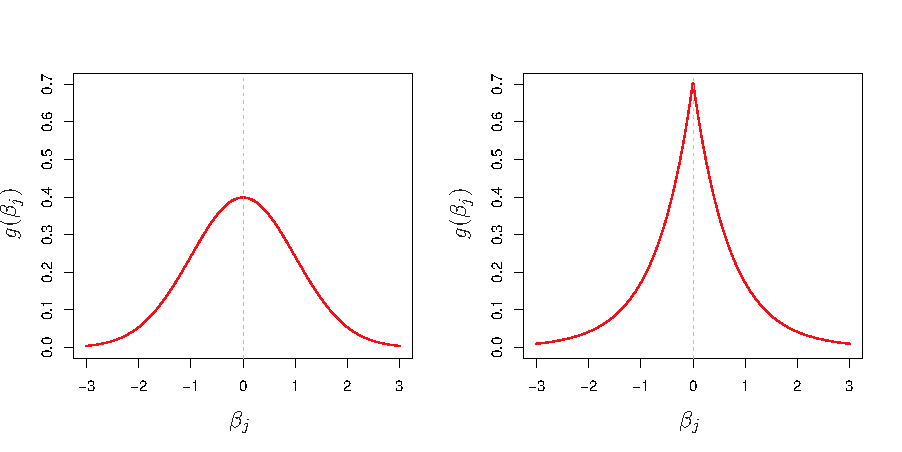
\includegraphics[scale=0.85]{../img/ISLR_ch6_fig11}
	\caption{Both Ridge and Lasso can be viewed as MAP estimators based on a Bayesian linear regression model. Whereas Ridge, at left, puts a normal prior on the regression coefficients, Lasso, at right, uses a Laplace prior, which has fatter tails and a taller peak at zero. This figure appears in Chapter 6 of James et al.\ (2013).}
	\label{fig:ridge_lasso_prior}
\end{figure}

When $p=2$, we can draw a picture of both the Ridge and Lasso problems in their ``budget constraint'' form. Both have the same objective function, which is proportional to the normal likelihood and describes a set of elliptical contours in $(\beta_1,\beta_2)$ -- space, centered at the MLE. Whereas Ridge has a circular constraint set, however, Lasso has a diamond-shaped one. Figure \ref{fig:ridge_lasso_constraint} shows how this difference in penalty functions leads to very different results. Sometimes the likelihood surface will hit a ``corner'' of the Lasso constraint set, leading to a zero coefficient estimate. In contrast, the Ridge constraint set has no corners and since it's circular there's nothing ``special'' about points on either axis.

\begin{figure}
	\centering
	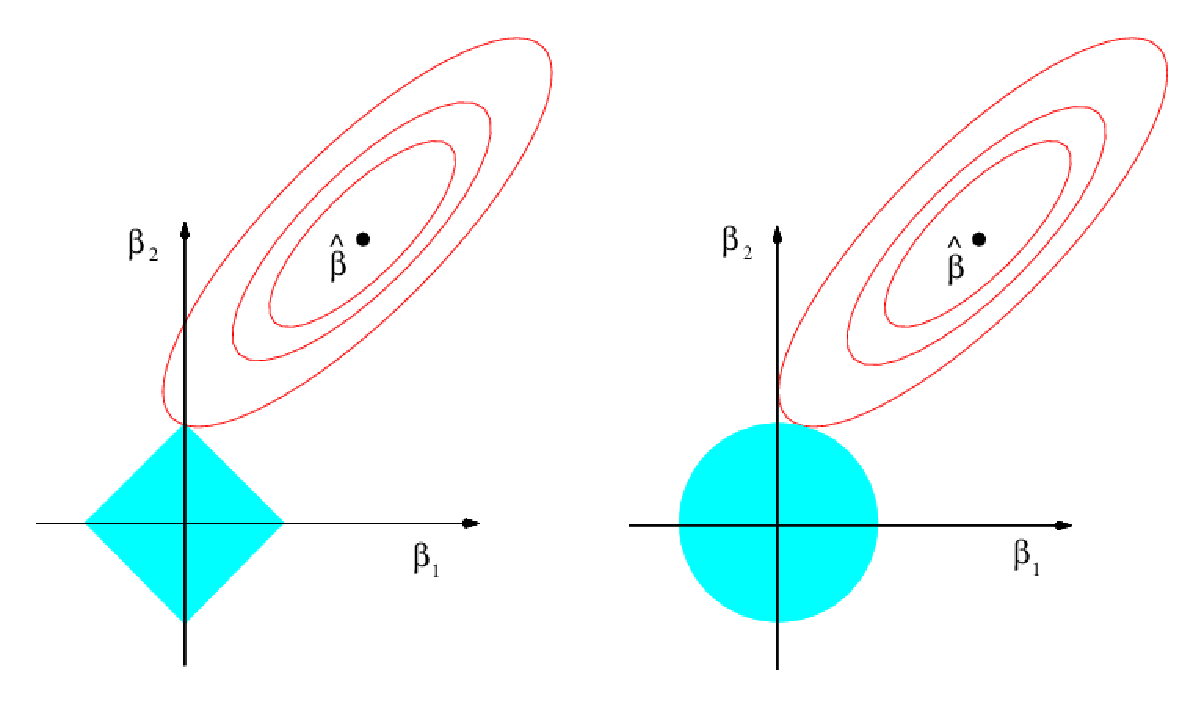
\includegraphics[scale=0.6]{../img/ISLR_ch6_fig7}
	\caption{In each panel $\widehat{\beta}$ denotes the MLE and the ellipses represent the contours of the likelihood. Both Lasso, at left, and Ridge, at right, shrink towards zero and away from the MLE. Because of its diamond-shaped constraint set, however, Lasso leads to a sparse solution, whereas Ridge does not. This figure appears in Chapter 6 of James et al (2013).}
	\label{fig:ridge_lasso_constraint}
\end{figure}

Yet another way to understand the difference between Ridge and Lasso is algebraically. For simplicity, and without loss of generality, suppose that $X$ is orthonormal. Another way of putting this is, suppose that we've replaced $X$ with its principal components. In this special case, it turns out that we can derive a closed form solution for Lasso. First we'll find the MLE. Since $X'X = I$, we have
	$$\widehat{\beta}_{MLE} = (X'X)^{-1}X'\textbf{y} = X'\textbf{y}$$
or written elementwise,
	$$\widehat{\beta}^{MLE}_j = \sum_{i=1}^n x_{ij}y_i$$
Similarly, for Ridge Regression we have
	$$\widehat{\beta}_{Ridge} =\left(X'X + \lambda I_p \right)^{-1}X'y = \left(I_p + \lambda I_p \right)^{-1} \widehat{\beta}_{MLE}$$
hence
	$$\widehat{\beta}^{Ridge}_j =  \left(\frac{1}{1+\lambda}\right)\widehat{\beta}^{MLE}_j$$
The calculations for Lasso are a bit more involved since there is no closed-form solution. We're trying to solve
	$$\underset{\beta}{\arg \min} (\mathbf{y}  - X\beta)' (\mathbf{y} - X\beta) + \lambda \left| \left| \beta\right| \right|_1$$
Now using $X'X = I$ along with $\widehat{\beta}_{MLE} = X'\textbf{y}$, we can expand the first term as
	\begin{eqnarray*}
		 (\mathbf{y}  - X\beta)' (\mathbf{y} - X\beta) &=& \mathbf{y}'\mathbf{y} - 2\beta' X' \mathbf{y} + \beta' X'X \beta \\
		 	&=& (\mbox{constant}) - 2\beta' \widehat{\beta}_{MLE} + \beta'\beta
	\end{eqnarray*}
Thus, for the case of orthonormal regressors we have:
\begin{eqnarray*}
	\widehat{\beta}_{Lasso} &=& \underset{\beta}{\arg \min} (\beta'\beta - 2\beta' \widehat{\beta}_{MLE})  +  \lambda \left| \left| \beta\right| \right|_1\\
		&=& \underset{\beta}{\arg \min}  \sum_{j=1}^p \left(\beta_j^2 - 2 \beta_j \widehat{\beta}^{MLE}_j + \lambda\left|\beta_j \right|\right)
\end{eqnarray*}
Here's the key: because the regressors are orthonormal, the optimization problem has been ``de-coupled.'' Since each $\beta_j$ only appears in one term of the sum, we can solve the overall optimization problem by solving $p$ \emph{completely independent} optimization problems:
	$$\widehat{\beta}^{Lasso}_j = \underset{\beta_j}{\arg \min} \left(\beta_j^2 - 2 \beta_j \widehat{\beta}^{MLE}_j + \lambda\left|\beta_j \right|\right)$$
Each of these $p$ objective functions has three terms. The first and third are always positive: they depend only on the absolute magnitude of $\beta_j$. In contrast, the second term could be either positive or negative depending on the signs of $\widehat{\beta}^{MLE}_j$ and $\beta_j$. Now, $\widehat{\beta}^{MLE}_j$ is outside our control: it's simply a function of the data. And whatever the \emph{magnitude} of $\beta_j$ changing its sign will not effect either $\beta_j^2$ or $\lambda|\beta_j|$. It follows that since we want to \emph{minimize} the criterion, we should \emph{match} the sign of $\beta_j$ to that of $\widehat{\beta}^{MLE}_j$. This ensures that the second term is negative. Accordingly, we consider two cases. 

\paragraph{Case I: $\widehat{\beta}^{MLE}_j >0$} As explained above we need to match the sign of $\beta_j$ to that of the MLE. Thus, we must have $\beta_j > 0$. Since $\beta_j >0$, it follows that $|\beta_j| = \beta_j$ and the problem becomes
	$$\widehat{\beta}^{Lasso}_j = \underset{\beta_j}{\arg \min} \; \beta_j^2 - 2 \beta_j \widehat{\beta}^{MLE}_j + \lambda\beta_j$$
Now that that pesky absolute value is gone, this is a straightforward calculus problem. The first order condition is $2\beta_j + \lambda = 2 \widehat{\beta}^{MLE}_j$. Solving, we have
	$$\beta_j = \widehat{\beta}^{MLE}_j - \frac{\lambda}{2}$$
But we're not quite done: we need $\beta_j > 0$ but the preceding expression will give a \emph{negative} value for $\beta_j$ if $\lambda$ is big enough. To keep this from happening, our corner solution must be to set $\beta_j = 0$ in this case. In other words, we have
	$$\widehat{\beta}^{Lasso}_j = \left(\widehat{\beta}^{MLE}_j - \frac{\lambda}{2} \right)_+ = \mbox{sign}\left(\widehat{\beta}^{MLE}_j \right)\left(\left| \widehat{\beta}^{MLE}_j\right| - \frac{\lambda}{2} \right)_+$$

\paragraph{Case II: $\widehat{\beta}^{MLE}_j \leq 0$} In this case, we must have $\beta_j \leq 0$ to match the sign of the MLE. It follows that $|\beta_j| = -\beta_j$ so the problem becomes
$$\widehat{\beta}^{Lasso}_j = \underset{\beta_j}{\arg \min} \; \beta_j^2 - 2 \beta_j \widehat{\beta}^{MLE}_j - \lambda\beta_j$$
The first order condition is $2\beta_j = 2\widehat{\beta}^{MLE}_j +\lambda$. Solving,
	$$\widehat{\beta}_j = \widehat{\beta}^{MLE}_j + \frac{\lambda}{2}$$
In this case we need $\beta_j <0$, just like $\widehat{\beta}^{MLE}_j$. But if $\lambda$ is sufficiently large, this requirement will be violated. To keep this from happening, our corner solution is, again, $\beta_j = 0$. We can express this as 
	$$\widehat{\beta}^{Lasso}_j =\mbox{sign}\left(\widehat{\beta}^{MLE}_j \right)\left(\left| \widehat{\beta}^{MLE}_j\right| - \frac{\lambda}{2} \right)_+$$
Hooray! We got the same answer in each case! To summarize, provided that $X$ is orthonormal, the Ridge and Lasso estimators are as follows:
	\begin{eqnarray*}
		\widehat{\beta}^{Ridge}_j &=&  \left(\frac{1}{1+\lambda}\right)\widehat{\beta}^{MLE}_j\\
		\widehat{\beta}^{Lasso}_j &=&\mbox{sign}\left(\widehat{\beta}^{MLE}_j \right)\left(\left| \widehat{\beta}^{MLE}_j\right| - \frac{\lambda}{2} \right)_+
	\end{eqnarray*}
Figure \ref{fig:ridge_lasso_shrink} depicts the difference between these two procedures. Whereas Ridge shrinks each element of $\widehat{\beta}_{MLE}$ by the same \emph{proportion}, namely $1/(1+\lambda)$, Lasso sets any elements of $\widehat{\beta}_{MLE}$ that are less than $\lambda/2$ to zero and \emph{translates} all other elements by a constant distance $\lambda/2$. 



\begin{figure}
	\centering
	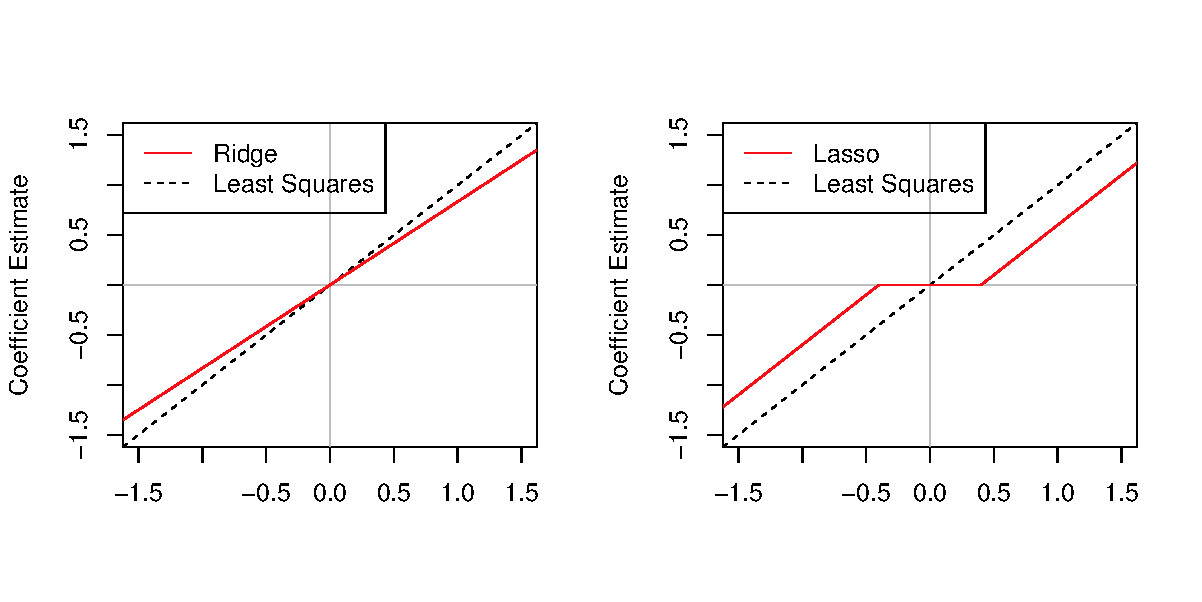
\includegraphics[scale=0.7]{../img/ISLR_ch6_fig10}
	\caption{These plots illustrate Ridge and Lasso shrinkage for the special case of orthonormal regressors. The horizontal axis in each plot is the MLE, while the vertical axis is the shrinkage estimator. Ridge appears at left and Lasso at right. The dashed 45-degree line in each plot corresponds to zero shrinkage. This figure appears in Chapter 6 of James et al (2013).}
	\label{fig:ridge_lasso_shrink}
\end{figure}

\subsection{Effective Degrees of Freedom for Lasso}
For a given value of $\lambda$ how complex is the corresponding Ridge fit compared to the Lasso fit? Is there a way for us to express these very different procedures in common units? We argued above that a reasonable measure of the complexity of Ridge Regression by $H(\lambda) = \mbox{trace}\left\{ X(X'X + \lambda I_p)^{-1} X'\right\}$. Since Lasso doesn't, in general, have a closed form it's not immediately clear what the appropriate analogy should be. It turns out (Zou, Hastie \& Tibshirani; 2007) that the the \emph{number of nonzero fitted coefficients} provides an unbiased estimator of effective degrees of freedom for Lasso. 

A cautionary note: two recent papers suggest that there are some complications in the analogy by which ``effective degrees of freedom'' in regularized regression are compared to parameter counts in ordinary regression. I haven't had a chance to look at these in detail yet, so if you're particularly keen you should write up a nice summary and send it to me! The papers are: Kaufman \& Rosset (2013) and Janson, Fithian \& Hastie (2013).

\subsection{How to Choose $\lambda$ for LASSO?}
Unlike Ridge, there's no computational shortcut for leave-one-out cross-validation that we can apply to Lasso. We can still use this procedure, but we have to do it the hard way. Of course we could also use $k$-fold cross-validation. But what about those model selection criteria we studied earlier in the semester? Is it possible to say anything about AIC, AIC$_C$, BIC, and $C_p$ in the context of Lasso estimation? The answer turns out to be \emph{yes} and many familiar properties carry over. Flynn, Hurvich and Simonoff (2013) show that the natural extensions of AIC, AIC$_C$ and $C_p$ to Lasso, using the effective degrees of freedom in place of the number of parameters, are asymptotically efficient. In a simulation study, they find that AIC, BIC and $C_p$ sometimes select values of $\lambda$ that are far too small: they ``catastrophically overfit.'' In contrast, AIC$_C$ performs well, just as it did in the case of ordinary linear regression. 

There is also a literature on the appropriate choice of $\lamba$ in settings where we hope to use Lasso to carry out variable selection. See the book \emph{Statistics for High-Dimensional Data} by B\"{u}hlmann and van de Geer (2011) for details and further references.


\subsection{Elastic Net}
There are arguments in favor of Ridge, and there are arguments in favor of Lasso. So why not try combining them? This is precisely the idea behind the so-called \emph{elastic net}. Rather than an $L_1$ or squared $L_2$-norm penalty, the elastic net uses
	$$\lambda \sum_{i=1}^p \left(\alpha \beta_j^2 + (1-\alpha)|\beta_j| \right)$$
The tuning parameter $\alpha$ controls ``how close'' the elastic net is to Ridge Regression. When $\alpha = 1$, we have Ridge. When $\alpha = 0$ we have Lasso. For any value in between, we have a combination of the two. For more on the elastic net, see Murphy (2013; Section 13.5.3).

% \subsection{Group LASSO}

% \subsection{Fused LASSO}

% \subsection{Inference for LASSO}
% All of this regularized linear regression stuff sounds great: it's computationally efficient and helps us make more reasonable predictions in a ``data-rich'' environment. But what if we want to carry out \emph{inference} for these models? Is there a simple way to proceed? 

% One option is go Bayesian: as long as we can sample from the posterior, we can construct credible intervals for any quantity of interest. Indeed, if we follow Park \& Casella and put a hyper-prior on ... we can even take uncertainty in the choose of smoothing parameter into account by integrating it out! 

% Things are much more complicated for Frequentists.

% Could go Bayesian. For a Frequentist, this is a very hard problem. A couple of recent papers, including Belloni et al.

\subsection{The Bayesian Lasso}
As mentioned above, the Lasso can be viewed as the MAP estimator from a Bayesian regression model with a Laplace prior, treating the error variance as known. The posterior mode, however, is a somewhat less than ideal summary. If forced to summarize a posterior using a single number we'd typically be much more comfortable with the mean or median. Park and Casella (2008) propose fully Bayesian version of the Lasso using a conditional Laplace prior for $\beta$ and a noninformative, scale-invariant prior for the error variance $\sigma^2$. Using the marginal likelihood to select $\lambda$, the posterior mean provides an estimator that is not exactly sparse, but appears to represent a compromise between Ridge and Lasso. By writing the Laplace distribution as a exponential scale mixture of normals, they show how to Gibbs sample the model and additionally consider inference and hyperpriors for $\lambda$.


\section{Shrinkage Estimation Using R}
Chapter 6 of James et al.\ (2013) ends with three ``Labs'' illustrating how to carry out various model selection and shrinkage procedures in R. The second and third of these contain Ridge Regression, Lasso, and PCR. There are some errors in the code as it appears in the book, so I've put together a corrected version with extensive comments called \texttt{ISLR\_ch6\_lab.R} and posted it in the GitHub repository for this class: \url{https://github.com/fditraglia/econ722}. This code makes heavy use of the excellent \texttt{GLMNET} package for R which is documented in Friedman, Hastie \& Tibshirani (2010). If you want to do your calculations using Matlab I'm afraid I can't offer you any guidance on the appropriate packages but if you send me some details, I'll include them in future versions of this document.

%!TEX root = ../main.tex
\chapter{Classical Factor Analysis and PCA}

This chapter draws on material from Chapters 11--12 of Murphy's \emph{Machine Learning: A Probabilistic Perspective}, Andrew Ng's lecture notes for CS229 at Stanford, and Jolliffe's \emph{Principal Component Analysis}.

\section{EM Algorithm}


\subsection{The Idea behind the EM Algorithm}
For simplicity, we'll consider an iid setup for now although the EM can be used in situations with dependence. We'll also suppose that the latent variable is continuous. If it's discrete the idea is exactly the same but the integral is replaced by a sum.
	$$\ell(\theta) = \sum_{t=1}^T \log p(\textbf{x}_t;\theta) = \sum_{t=1}^T \log \left(\int p(\textbf{x}_t,	\textbf{z}_t;\theta)\; d \textbf{z} \right)$$
where $\mathbf{x}_t$ is observed and $\mathbf{z}_t$ is unobserved. In many interesting models there is no explicit formula for the MLE in terms of the marginal density $p(\mathbf{x}_t;\theta)$ but there \emph{is} an explicit formula in terms of the \emph{joint} density $p(\mathbf{x}_t,\mathbf{z}_t;\theta)$. This is exactly the setting in which the EM algorithm is useful. Rather than directly maximizing $\ell(\theta)$, the EM algorithm proceeds \emph{iteratively} over the following two steps:
	\begin{description}
		\item[(E-step)] Construct a \emph{lower bound} for $\ell(\theta)$
		\item[(M-step)] Optimize the lower bound over $\theta$
	\end{description}
Roughly speaking, the EM algorithm converts a single complicated optimization problem into a sequence of simple optimization problems. The trick is to ensure that the resulting sequence of estimators converges to the MLE. Jensen's Inequality is the key so I'll briefly remind you of a few importnat facts before proceeding. 

\begin{figure}
	\centering
	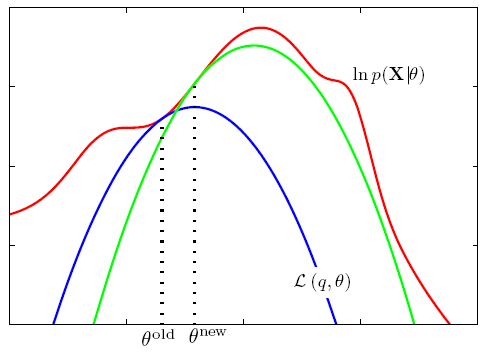
\includegraphics[scale=0.5]{../img/EM_algorithm}
	\caption{Illustration of the EM Algorithm: to maximize the log likelihood, the red curve, we create a sequence of successive approximations, the blue and green curves, and maximize these. This appears as Figure 9.14 in Bishop's (2006) \emph{Pattern Recognitiion and Machine Learning}.}
\end{figure}

\subsection{Jensen's Inequality}
Recall that a function is called \emph{convex} if its Hessian matrix is positive semi-definite and \emph{strictly convex} if its Hessian matrix is positive definite. For functions of a single variable the condition is $f''(x)\geq 0 \quad \forall x\in\mathbb{R}$ for \emph{convex} and $f''(x)> 0 \quad \forall x\in\mathbb{R}$ for \emph{strictly convex}. In statistics, one of the most useful results concerning convex functions is \emph{Jensen's Inequality}
\begin{pro}[Jensen's Inequality]
 	Let $f$ be a convex function and $X$ be a random variable. Then $E[f(X)]\geq f(E[X])$. If $f$ is strictly convex then the inequality is strict unless $P(X = E[X]) = 1$, i.e.\ $X$ is a constant. For the equivalent results for concave functions, simply reverse the inequality.
 \end{pro} 



\subsection{A Lower Bound for the Likelihood}
Let $f_t(\mathbf{z}_t)$ be \emph{some arbitrary} density function over the support of $\mathbf{z}_t$, that is any function satisfying $f_t(\mathbf{z_t})\geq 0$ and
	$$\int f_t(\textbf{z}_t) \;d \textbf{z}_t = 1$$
We have
	\begin{eqnarray*}
		 \ell(\theta) = \sum_{t=1}^T \log p(\textbf{x}_t;\theta) &=& \sum_{t=1}^T \log \left(\int p(\textbf{x}_t,	\textbf{z}_t;\theta)\; d \textbf{z}_t \right)\\
		 	&=&  \sum_{t=1}^T \log \left(\int f_t(\mathbf{z}_t) \left[\frac{p(\textbf{x}_t,	\textbf{z}_t;\theta)}{f_t(\mathbf{z}_t)}\right] d \textbf{z}_t \right)
	\end{eqnarray*}
Now we use Jensen's inequality and the fact that $\log$ is a concave function over its domain to find that
	$$\log \left(\int f_t(\mathbf{z}_t) \left[\frac{p(\textbf{x}_t,	\textbf{z}_t;\theta)}{f_t(\mathbf{z}_t)}\right] d \textbf{z}_t \right) \geq \int f_t(\mathbf{z}_t) \log\left[\frac{p(\textbf{x}_t,\textbf{z}_t;\theta)}{f_t(\mathbf{z}_t)}\right] d \textbf{z}_t $$
What's going on here? Since $f_t$ is a \emph{density} the integral inside the parentheses is \emph{an expectation} of a particular function of the argument of integration $\mathbf{z}_t$. The parameter $\theta$ and the observed vector of realizations $\mathbf{x}_t$ are constants with respect to the integration. Substituting the preceding inequality into the sum, we have established that
	$$\ell(\theta) \geq \sum_{t=1}^T \left(\int f_t(\mathbf{z}_t) \log\left[\frac{p(\textbf{x}_t,\textbf{z}_t;\theta)}{f_t(\mathbf{z}_t)}\right] d \textbf{z}_t \right)$$
for \emph{any} density function $f_t$. This is the \emph{lower bound} for the likelihood that we will use in the E-step. The question is, how should we choose $f_t$? 

The key idea is to turn the \emph{inequality} into an \emph{equality} at a particular value of $\theta$. Intuitively, we want to ensure that, in a given iteration of the algorithm, the  actual likelihood and the lower bound \emph{agree} at the value of $\theta$ that emerged from the \emph{preceding} iteration. In this way, our sequence of approximating functions will ``trace out a path'' along the true likelihood, ultimately ensuring that the EM algorithm will converge to the MLE. Since $\log$ is in fact \emph{strictly} concave, the only way for Jensen's inequality to hold with equality is if 
$$\frac{p(\textbf{x}_t,\textbf{z}_t;\theta)}{f_t(\mathbf{z}_t)} = c$$
for some constant $c$ that \emph{does not depend} on $\mathbf{z}_t$. The question is, how should we choose $f_t$ to achieve this? Rearranging, integrating, and using the fact that $f_t$ is a density,
	\begin{eqnarray*}
		c f_t(\mathbf{z}_t) &=& p(\mathbf{x}_t, \mathbf{z}_t;\theta)\\
		c \int f_t(\mathbf{z}_t) \; d \mathbf{z}_t &=& \int p(\mathbf{x}_t, \mathbf{z}_t;\theta) \; d \mathbf{z}_t\\
		c &=& p(\mathbf{x}_t;\theta) 
	\end{eqnarray*}
Substituting for $c$, solving for $f_t$ and using the definition of a conditional density we have
	$$f_t(\textbf{z}_t)= \frac{p(\textbf{x}_t,\textbf{z}_t;\theta)}{p(\mathbf{x}_t;\theta)} = p(\textbf{z}_t|\textbf{x}_t;\theta)$$
In other words, to make the lower bound hold with equality at a particular value of $\theta$, say $\theta^*$, it suffices to set $f_t$ equal to the \emph{conditional} density of $\mathbf{z}_t$ \emph{given} $\mathbf{x}_t$ \emph{evaluated} at $\theta^*$. Crucially this is a both a probability density and a function of $\mathbf{z}_t$ \emph{only} since we plug in the observed value of $\mathbf{x}_t$.

\subsection{The Algorithm}
In the previous subsection we showed that if we set $f_t(\mathbf{z}_t) = p(\textbf{z}_t|\textbf{x}_t;\theta^*)$ then
	$$\ell(\theta^*) = \sum_{t = 1}^T  \left(\int f_t(\mathbf{z}_t) \log\left[\frac{p(\textbf{x}_t,\textbf{z}_t;\theta^*)}{f_t(\mathbf{z}_t)}\right] d \textbf{z}_t \right)$$
and, more generally for \emph{any} value of $\theta$
	$$\ell(\theta) \geq \sum_{t = 1}^T  \left(\int f_t(\mathbf{z}_t) \log\left[\frac{p(\textbf{x}_t,\textbf{z}_t;\theta)}{f_t(\mathbf{z}_t)}\right] d \textbf{z}_t \right)$$
by Jensen's Inequality. Now we are ready to state the EM algorithm:
\begin{alg}[EM Algorithm]
First select a starting value $\theta^{(1)}$. Then repeat the following two steps repeatedly until convergence
			\begin{description}
			 	\item[(E-step)] For each $t$ set $f_t^{(j-1)}(\mathbf{z}_t) = p(\mathbf{z}_t|\mathbf{x}_t; \theta^{(j-1)})$ where $\theta^{(j-1)}$ is the solution from the M-step of the \emph{preceding} iteration. 
			 	\item[(M-step)] 
			 		$\displaystyle\theta^{(j)} = \underset{\theta \in \Theta}{\arg \max} \sum_{t = 1}^T  \left(\int f_t^{(j-1)}(\mathbf{z}_t) \log\left[\frac{p(\textbf{x}_t,\textbf{z}_t;\theta)}{f_t^{(j-1)}(\mathbf{z}_t)}\right] d \textbf{z}_t \right)$
			 \end{description}
If $j = 2$ then $\theta^{(j-1)}$ is simply the starting value $\theta^{(1)}$.
\end{alg}
Note that in the M-step the argument $\theta$ over which we maximize \emph{only} enters the expression $p(\textbf{x}_t,\textbf{z}_t;\theta)$. The density $f^{(j-1)}(\mathbf{z}_t)$ does \emph{not} depend on $\theta$, it depends on the \emph{constant} $\theta^{(j-1)}$ that solved the M-step of the \emph{previous iteration}. The amazing thing about the EM algorithm is that it is \emph{guaranteed} to converge to a local maximum of the likelihood function: each successive iteration \emph{monotonically} improves the likelihood as we will see below. This fact along the the way we constructed our lower bound to hold with equality at the value of $\theta$ from the \emph{previous} M-step gives us an excellent tool for debugging our code: simply plot
	$$\ell(\theta^{(j)}) = \sum_{t = 1}^T  \left(\int f_t^{(j)}(\mathbf{z}_t) \log\left[\frac{p(\textbf{x}_t,\textbf{z}_t;\theta^{(j)})}{f_t^{(j)}(\mathbf{z}_t)}\right] d \textbf{z}_t \right)$$ 
against $j$. The preceding expression is the \emph{objective function} from the $(j+1)$th M-step evaulated at the \emph{solution} from the $j$th M-step. By construction, this If the is equal to the likelihood evaulated at $\theta^{(j)}$. If the plot is \emph{not} increasing monotonically in $j$, then there must be a bug in your code.

\subsection{Why Does the EM Algorithm Converge?}
Let $\theta^{(j)}$ and $\theta^{(j+1)}$ be two succesive solutions to the M-step of the EM algorithm. We will now show that $\ell(\theta^{(j)}) \leq \theta^{(j+1)}$. In other words, the EM algorithm \emph{monotonically} improves the likelihood in each iteration. Since $\{\theta^{(j)}\}$ is a monotonic sequence, it converges as long as it is bounded (Rudin Theorem 3.14). Since $\ell(\theta^{(1)})$ is a lower bound, if follows that the EM algorithm is \emph{guaranteed} to converge to a local maximum of the likelihood function provided that the likelihood function is bounded above. All that remains is to actually demonstrate that $\ell(\theta^{(j)}) \leq \theta^{(j+1)}$.

By definition, 
	$$\theta^{(j+1)} = \underset{\theta \in \Theta}{\arg \max} \sum_{t = 1}^T  \left(\int f_t^{(j)}(\mathbf{z}_t) \log\left[\frac{p(\textbf{x}_t,\textbf{z}_t;\theta)}{f_t^{(j)}(\mathbf{z}_t)}\right]d \textbf{z}_t \right)$$ 
Now let $\tilde{\theta}$ be some arbitrary value of $\theta$. Since $\theta^{(j+1)}$ is the $\arg \max$, evaluating the objective function at $\tilde{\theta}$ cannot yield a greater value than evaluating it at $\theta^{(j+1)}$. Since this holds for \emph{any} $\tilde{\theta}$ it holds in particular for $\theta^{(j)}$. Hence, 
	\begin{eqnarray*}
		\sum_{t = 1}^T  \left(\int f_t^{(j)}(\mathbf{z}_t) \log\left[\frac{p(\textbf{x}_t,\textbf{z}_t;\theta^{(j+1)})}{f_t^{(j)}(\mathbf{z}_t)}\right] d \textbf{z}_t \right) 
		&\geq& 
		\sum_{t = 1}^T  \left(\int f_t^{(j)}(\mathbf{z}_t) \log\left[\frac{p(\textbf{x}_t,\textbf{z}_t;\theta^{(j)})}{f_t^{(j)}(\mathbf{z}_t)}\right] d \textbf{z}_t \right)\\
		&=& \ell(\theta^{(j)})
	\end{eqnarray*}
since we chose $f^{(j)}_t(\mathbf{z}_t)$ to make Jensen's Inequality strict at $\theta^{(j)}$. Now, recall from above that for \emph{any density} $f_t(\mathbf{z}_t)$ and \emph{any} value of $\theta$,
	$$\ell(\theta) \geq \sum_{t=1}^T \left(\int f_t(\mathbf{z}_t) \log\left[\frac{p(\textbf{x}_t,\textbf{z}_t;\theta)}{f_t(\mathbf{z}_t)}\right] d \textbf{z}_t \right)$$
by Jensen's Inequality. Since this holds in general, it also holds in particular for $\theta = \theta^{(j+1)}$ and $f_t(\mathbf{z}_t)= f_t^{(j)}(\mathbf{z}_t)$. Hence,
	$$\ell(\theta^{(j+1)}) \geq \sum_{t=1}^T \left(\int f_t^{(j)}(\mathbf{z}_t) \log\left[\frac{p(\textbf{x}_t,\textbf{z}_t;\theta^{(j+1)})}{f_t^{(j)}(\mathbf{z}_t)}\right] d \textbf{z}_t \right)$$
Combining the two inequalities gives $\ell(\theta^{(j+1)}) \geq \ell(\theta^{(j)})$ as claimed.


\section{Factor Analysis}

Before we proceed, I'll just remind you of some key facts about normal distributions and we'll need below.

\subsection{Facts about the Multivariate Normal Distribution}
\subsubsection{Linear Combinations}
Suppose that $X \sim N(\mu, \Sigma)$ and $Y = a + BX$ where $a$ is a vector and $B$ a matrix of constants. Then $Y \sim (a + B\mu, B\Sigma B')$.
\subsubsection{Marginals and Conditionals}
Let $X_1$ and $X_2$ be random vectors such that $(X_1' , X_2') \sim N(\mu, \Sigma)$ where
	$$\mu = \left[\begin{array}{c}
		\mu_1 \\ \mu_2
	\end{array}\right], \quad \Sigma = \left[ \begin{array}{cc}
	\Sigma_{11} & \Sigma_{12}\\
	\Sigma_{21} & \Sigma_{22}
	\end{array}\right]
	$$
Then, 
	\begin{eqnarray*}
		X_1 &\sim& N(\mu_1, \Sigma_{11})\\
		X_2 &\sim& N(\mu_2, \Sigma_{22})\\
		X_1|X_2 &\sim& N(\mu_{1|2}, \Sigma_{1|2})
	\end{eqnarray*}
where,
	\begin{eqnarray*}
		\mu_{1|2} &=& \mu_1 + \Sigma_{12}\Sigma_{22}^{-1}(X_2 - \mu_2)\\
		\Sigma_{1|2} &=&\Sigma_{11} - \Sigma_{12} \Sigma_{22}^{-1} \Sigma_{21}
	\end{eqnarray*}

\subsection{The Factor Analysis Model}
Classical Factor Analysis specifies a joint distribution on the observable random $p$-vector $X$ and an unobserved or ``latent'' random $k$-vector $Z$, as follows
	\begin{eqnarray*}
		Z &\sim& N_k(0_k, \mathbf{I}_k)\\
		\epsilon &\sim& N_p(0_p, \Psi)\\
		Z &\perp& \epsilon\\
		X &=& \mu + \Lambda Z + \epsilon
	\end{eqnarray*}
where $\mu$ is a $p\times 1$ vector of parameters, $\Lambda$ is a $p\times k$ matrix of parameters called the \emph{factor loading matrix}, and $\Psi$ is a $p\times p$ \emph{diagonal} matrix of parameters. Factor Analysis can be viewed as a ``low rank parameterization'' of a multivariate normal distribution. The idea is that, while $X$ is a random $p$-vector, its realizations lie \emph{close} to a $k$-dimensional affine subspace: $\Lambda$ maps $Z$ from $\mathbb{R}^k$ to a linear subspace of $\mathbb{R}^p$, $\mu$ shifts this subspace away from the origin, and $\epsilon$ adds axis-aligned Gaussian noise. Hence it makes sense to require that $k$ is strictly less than both $p$, the dimension of $X$, and $T$, the sample size. 

The intution is as follows: Factor Analysis ``forces'' $Z$ to ``explain'' the correlation structure of $X$. This is why $\Psi$ is required to be diagonal. The diagonal elements of $\Psi$ are sometimes called the \emph{idiosyncratic variance terms}, since each corresponds to a \emph{single} component of $X$. This is the key point: \emph{conditional} on the factors $Z$, the elements of $X$ are \emph{independent}. 
\begin{figure}
	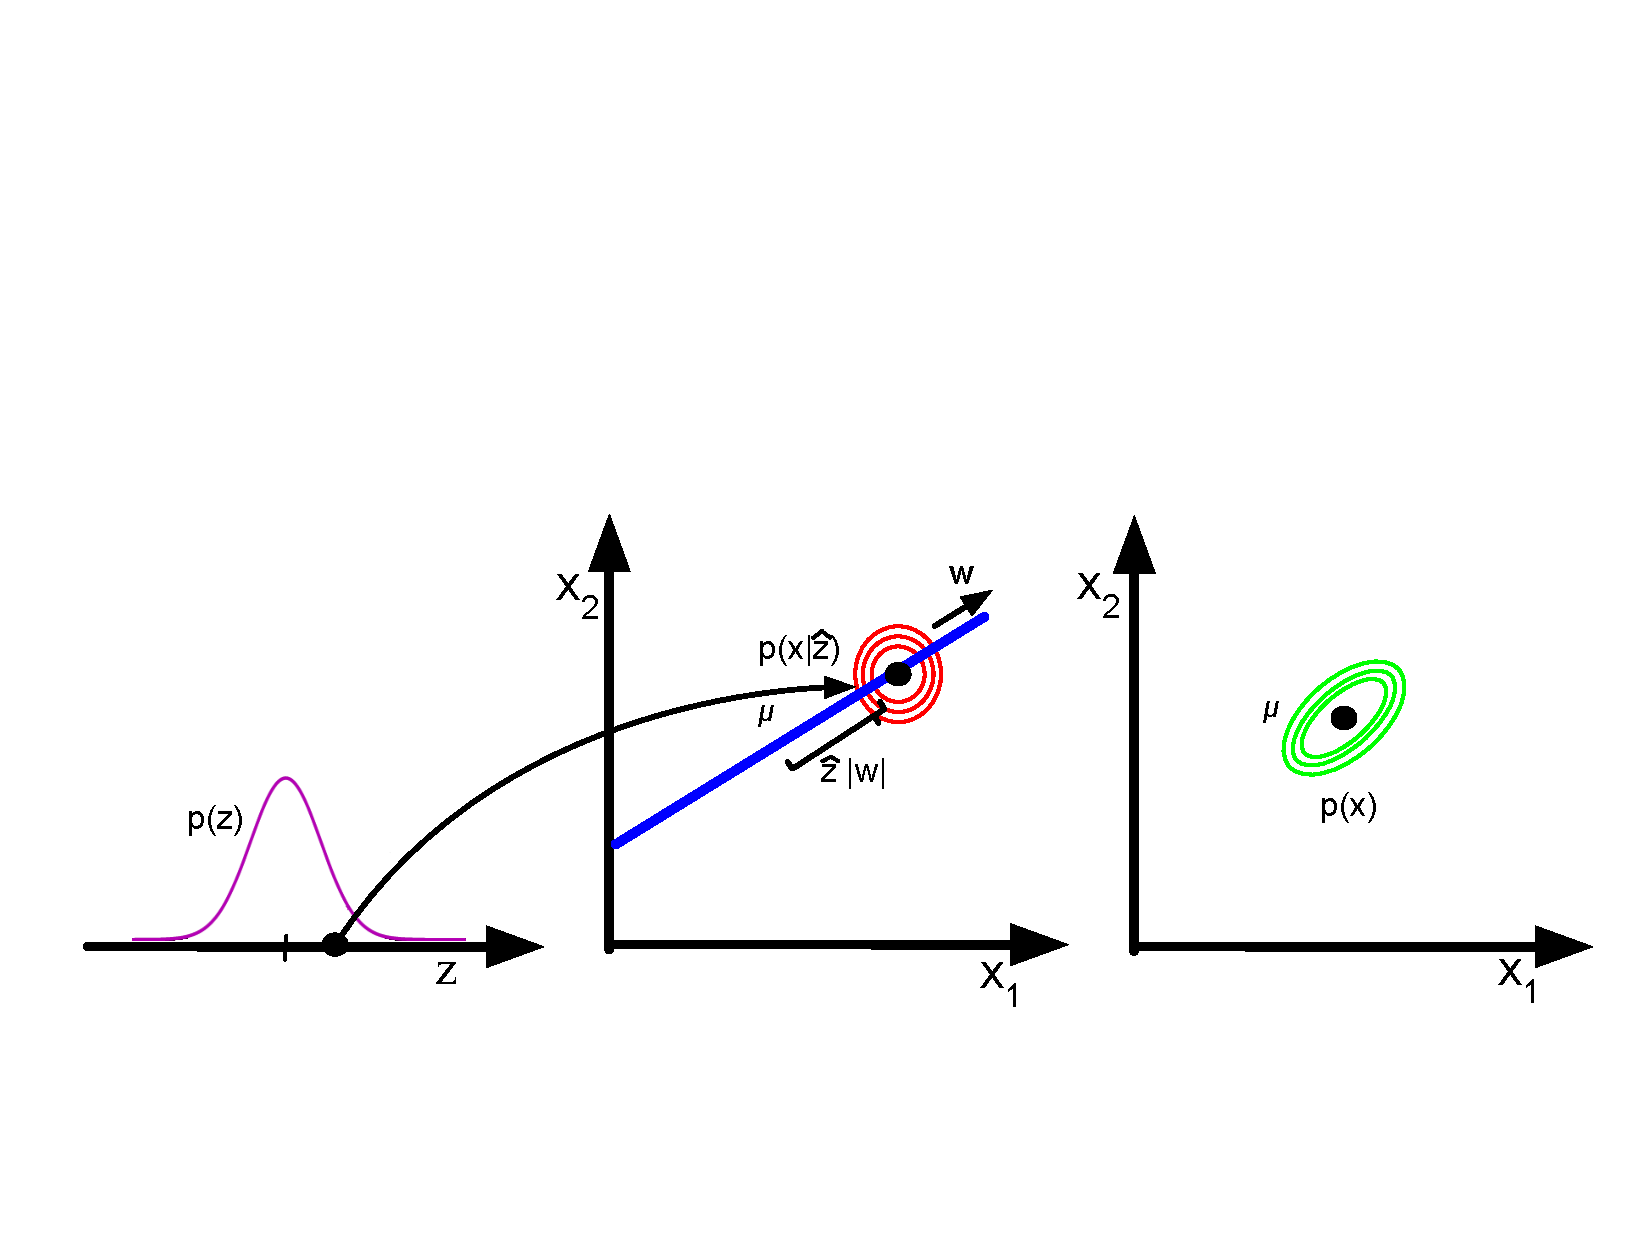
\includegraphics[scale=0.5]{../img/factor_analysis}
	\caption{Illustration of Factor Analysis, although the notation is slightly different from mine. (I need to draw my own version of this.) This appears as figure 12.1 in Murphy (2012).}
\end{figure}

The factor analysis model implies that the joint distribution of $Z$ and $X$ is normal. Specifically,
\begin{eqnarray*}
	\left[\begin{array}{c}
	Z\\ X
	\end{array}\right] &=& 
		\left[\begin{array}{c}
	0_k\\ \mu
	\end{array}\right] + \left[\begin{array}{cc}
		\mathbf{I}_k & 0_{k\times p} \\ \Lambda & I_{p}
	\end{array}\right]\left[\begin{array}{c}
		Z \\ \epsilon
	\end{array} \right]\\
	& = & \left[\begin{array}{c}
	0_k\\ \mu
	\end{array}\right] + \left[\begin{array}{cc}
		\mathbf{I}_k & 0_{k\times p} \\ \Lambda & I_{p}
	\end{array}\right]
	N\left(\left[\begin{array}{c}
		0_k \\ 0_p
	\end{array} \right], \left[\begin{array}{cc}
		\mathbf{I}_k & 0_{k\times p} \\ 0_{p\times k} & \Psi
	\end{array}\right]\right)\\
	&\sim & N\left(\left[\begin{array}{c}
	0_k \\ \mu
	\end{array}\right], \left[\begin{array}{cc}
		I & \Lambda'\\
		\Lambda & \Lambda \Lambda' + \Psi
	\end{array} \right] \right)
\end{eqnarray*}
The algebra for the variance matrix calculation is as follows:
	\begin{eqnarray*}
		V &=& \left[\begin{array}{cc}
		\mathbf{I}_k & 0_{k\times p} \\ \Lambda & I_{p}
	\end{array}\right]
\left[\begin{array}{cc}
		\mathbf{I}_k & 0_{k\times p} \\ 0_{p\times k} & \Psi
	\end{array}\right]
	\left[\begin{array}{cc}
		\mathbf{I}_k & 0_{k\times p} \\ \Lambda & I_{p}
	\end{array}\right]'\\
	&=& \left[ \begin{array}
		{cc} 
		\mathbf{I}_k & 0_{k\times p}\\
		\Lambda & \Psi
	\end{array}\right]\left[\begin{array}{cc}
		\mathbf{I}_k & \Lambda '\\
		0_{p\times k} & I_{p} 
	\end{array}\right]\\
	&=& \left[\begin{array}
		{cc}
		\mathbf{I}_k & \Lambda' \\
		\Lambda & \Lambda \Lambda' + \Psi
	\end{array}\right]
	\end{eqnarray*}


\subsection{The Factor Analysis Model is Not Identified}
Suppose we want to estimated the parameters $\mu, \Lambda, \Psi$ of the factor analysis model. The first natural question is whether this model is even identified. The mean vector $\mu$ doesn't provide any problems for identification since we can always demean $X$ before proceeding. Excluding $\mu$, the factor analysis model has $k(p + 1)$ free parameters: $\Lambda$ is a $p\times k$ matrix and $\Psi$ is a \emph{diagonal} $p\times p$ matrix.


Unfortunately the Factor Analysis is not identified as given above. To see why, suppose that $R$ is an orthogonal matrix, i.e.\ $RR' = R'R = I$. Geometrically, $R$ is a rotation: it leaves the length of any vector $v$ unchanged since
	$$|| Rv || = \sqrt{(Rv)'(Rv)} = \sqrt{v' R'R v} = \sqrt{v'v} = ||v||$$ 
And it leaves the \emph{distance} between any two vectors $v$ and $w$ unchanged since
	\begin{eqnarray*}
		||Rv - Rw|| &=& ||R(v-w)|| = \sqrt{\left[R(v-w) \right]' \left[ R(v-w)\right]}\\
			&=& \sqrt{(v-w)'R'R(v-w)} = \sqrt{(v-w)'(v-w)} = ||v-w||
	\end{eqnarray*}
From the joint distribution for $X$ and $Z$ that we derived above it follows that the marginal distribution of $X$ is $N(\mu, \Lambda \Lambda' + \Psi)$. Thus if we observe realizations $\mathbf{x}_1, \mathbf{x}_2, \hdots, \mathbf{x}_T$ of a sequence of iid random vectors $X_1, X_2, \hdots, X_T$ generated from the Factor Analysis model the log-likelihood is given by
	\begin{eqnarray*}
		\ell(\mu, \Lambda, \Psi) = \log \left[ \prod_{t = 1}^T \frac{\exp \left\{ -\frac{1}{2} \left(\mathbf{x}_t - \mu \right)' \left(\Lambda \Lambda' + \Psi \right)^{-1} \left(\mathbf{x}_t - \mu \right)\right\}}{(2\pi)^{p/2}\left| \Lambda \Lambda' + \Psi \right|^{1/2}} \right] 
	\end{eqnarray*}
Now suppose that we evaluate the log-likelihood at $\widetilde{\Lambda}R$ rather than $\Lambda$. Since $\Lambda$ only enters through the outer product $\Lambda \Lambda'$ the likelihood is \emph{unchanged}: 
	$$\widetilde{\Lambda} \widetilde{\Lambda}' = (\Lambda R)(\Lambda R)' = \Lambda RR' \Lambda' = \Lambda \Lambda'$$
We have shown that the matrix of factor loadings is \emph{only identified up to a rotation}. Another way to think about this is in terms of the latent variable $Z$, Since $X = \mu + \Lambda Z + \epsilon$, post-multiplying $\Lambda$ by $R$ is the same as \emph{pre-multiplying} $Z$ by $R$. As explained above, this constitutes a \emph{rotation} of the vector $Z$. But since $Z$ is a \emph{spherical} normal distribution, rotating it cannot change the likelihood.


If we merely plan to use Factor Analysis for \emph{prediction} this lack of identification is irrelevant: it does not affect the predictive performance of the model in any way. If we ultimately hope to \emph{interpret} the latent factors, however the lack of identification becomes problematic. There are various ways to get a unique solution for the factor loadings $\Lambda$ that involve making various restrictions on the matrix of factor loadings $\Lambda$. The first question is: so how many restrictions do we need?

Since the lack of identication comes from rotational invariance, we need to count the number of free parameters in a $k\times k$ rotation matrix. Start with the first column: it has $k-1$ free parameters since the only constraint is that it have length one. The second column must also have length one, but it has the further restriction that it must be orthogonal to the first column. Hence it has $k - 2$ free parameters. Continuing in this way, we see that there are $(k - 1) + (k - 2) + \hdots + (k - k + 1) = k(k-2)/2$ free parameters in a general $k\times k$ rotation matrix. 

There are a number of possible solutions to the lack of identification:
	\begin{itemize}
		\item \textbf{Constraining the columns of $\Lambda$ to be orthonormal} This is essentially how PCA works, as we'll see below.
		\item \textbf{Constraining $\Lambda$ to be lower triangular} This constraint imposes that the first element of $X$ only depends on the first factor, the second element of $X$ only depends on the first two factors, and so on. In this choice of which variables to list as the first elements of $X$ can make a \emph{big difference}.
		\item \textbf{Imposing Sparsity on $\Lambda$} There are a number of proposals for ``sparse factor analysis,'' including using LASSO and imposing an $\ell_1$ penalty on the factor loadings. Although this might not completely solve the identification problem, setting many of the elements of $\Lambda$ to exactly zero can partially resolve it. 
		\item \textbf{Choosing an Informative Rotation Matrix} If you read old textbooks on multivariate statistics, you'll see a number of suggestions, including something called the ``varimax'' method. Typically, these solutions involve some kind of sparsity condition.
		\item \textbf{Use a Non-Gaussian Distribution for the Factors} The lack of identification in the Factor Analysis Model comes from the rotational invariance of a multivariate normal distribution with an identity covariance matrix. Using a distribution other than the normal can partially eliminate this problem: a Laplace distribution, for example, has diamond-shaped contours. This is the idea behind ``Independent Components Analysis'' (ICA).
	\end{itemize}



\subsection{The Latent Factors}
The unobserved random variables $Z_1, \hdots, Z_T$ that generate $X_1, \hdots, X_T$ under the Factor Analysis Model are called the \emph{latent factors} or the \emph{latent scores}. In some settings the factor scores are given a particular interpretation and we may wish to infer them from the observable data. (Warning: interpreting the factors can be very difficult because of the lack of idenfication of the factor model!) Because this model is Gaussian, we can easily work out the conditional distribution of the latent factors using joint distribution of $(Z',X')'$. Indeed, this is precisely what we'll need to do to implement the EM algorithm, as we'll see below. 


\subsection{Deriving EM for Classical Factor Analysis}
This is a great problem for the EM algorithm since it can be viewed as a case of missing data: if $Z$ were observed, this would just be a standard multivariate regression problem!


\subsubsection{The E-step: Inferring the Latent Factors} In this step we set $f_t^{(j-1)}(\mathbf{z}_t) = p(\mathbf{z}_t|\mathbf{x}_t; \theta^{(j-1)})$ for each $t$ where $\theta^{(j-1)}$ is the value of $\theta$ that solved the optimization problem from the \emph{preceding} M-step or, if $j=2$, the starting value. In the notation of the factor analysis problem we need to calculate:
	$$f_t^{(j-1)}(\mathbf{z}_t) = p(\mathbf{z}_t | \mathbf{x}_t; \mu^{(j-1)}, \Lambda^{(j-1)}, \Psi^{(j-1)})$$
As we showed above,
	\begin{eqnarray*}
		\left[\begin{array}{c}
			Z\\ X
		\end{array}\right] 
		&\sim&  N\left(
		\left[\begin{array}{c}
			0_k \\ \mu
	\end{array}\right], 
		\left[\begin{array}{cc}
			I & \Lambda'\\
			\Lambda & \Lambda \Lambda' + \Psi
		\end{array} \right] \right)
	\end{eqnarray*}
Hence, using the properties of the normal distribution reviewed earlier in this document:
	\begin{eqnarray*}
		Z|X &\sim& N_k(\mu_{Z|X}, \Sigma_{Z|X})\\
		\mu_{Z|X} &=& \Lambda' (\Lambda \Lambda' + \Psi)^{-1}(X - \mu) \\
		\Sigma_{Z|X} &=& \mathbf{I}_k - \Lambda'(\Lambda \Lambda' + \Psi)^{-1}\Lambda
	\end{eqnarray*}
\subsubsection{The M-Step: Optimizing the Lower Bound}
In this step, we solve 
	$$\displaystyle\theta^{(j)} = \underset{\theta \in \Theta}{\arg \max} \sum_{t = 1}^T  \left(\int f_t^{(j-1)}(\mathbf{z}_t) \log\left[\frac{p(\textbf{x}_t,\textbf{z}_t;\theta)}{f_t^{(j-1)}(\mathbf{z}_t)}\right] d \textbf{z}_t \right)$$
Before carrying out the optimization problem, we'll first manipulate the objective function to simplify it and remove constant terms that don't depend on the model parameters. Substituting the notation of the Factor Analysis Model and rearranging, we can write the objective function for the $j$th M-step as follows:
	\begin{eqnarray*}
		Q^{(j)}(\mu, \Lambda, \Psi) &=& \sum_{t=1}^T \int f_t^{(j-1)}(\textbf{z}_t) \log \left[ \frac{p(\textbf{x}_t, \textbf{z}_t;\mu, \Lambda, \Psi)}{f_t^{(j-1)}(\textbf{z}_t)}\right] d \textbf{z}_t\\
			&=&	\sum_{t=1}^T \int f_t^{(j-1)}(\textbf{z}_t) \left[\log p(\textbf{x}_t, \textbf{z}_t;\mu, \Lambda, \Psi) - \log f_t^{(j-1)}(\textbf{z}_t)\right] d \textbf{z}_t\\
		&=&\sum_{t=1}^T \int f_t^{(j-1)}(\textbf{z}_t) \log p(\textbf{x}_t, \textbf{z}_t;\mu, \Lambda, \Psi)\;d \textbf{z}_t -\sum_{t=1}^T  \int f_t^{(j-1)}(\textbf{z}_t) \log f_t^{(j-1)}(\textbf{z}_t) \;d \textbf{z}_t\\
		&=&\sum_{t=1}^T \int f_t^{(j-1)}(\textbf{z}_t) \log p(\textbf{x}_t, \textbf{z}_t;\mu, \Lambda, \Psi)\;d \textbf{z}_t  + C\\
		&=& \sum_{t=1}^T \int f_t^{(j-1)}(\textbf{z}_t) \log p(\textbf{x}_t, \textbf{z}_t;\mu, \Lambda, \Psi)\;d \textbf{z}_t -\sum_{t=1}^T  \int f_t^{(j-1)}(\textbf{z}_t) \log f_t^{(j-1)}(\textbf{z}_t) \;d \textbf{z}_t\\
		&=&\sum_{t=1}^T \int f_t^{(j-1)}(\textbf{z}_t) \log\left[ p(\textbf{x}_t| \textbf{z}_t;\mu, \Lambda, \Psi)p(\textbf{z}_t) \right]d \textbf{z}_t  + C\\
		&=&\sum_{t=1}^T \int f_t^{(j-1)}(\textbf{z}_t) \log p(\textbf{x}_t| \textbf{z}_t;\mu, \Lambda, \Psi)\;d \textbf{z}_t + \sum_{t=1}^T \int f_t^{(j-1)}(\textbf{z}_t)\log p(\textbf{z}_t)\; d \mathbf{z}_t + C\\
		&=& \sum_{t=1}^T \int f_t^{(j-1)}(\textbf{z}_t) \log p(\textbf{x}_t| \textbf{z}_t;\mu, \Lambda, \Psi)\;d \textbf{z}_t + C
	\end{eqnarray*} 
where $C$ denotes an arbitrary constant and we have used the fact that $p(\mathbf{z}_t)$ \emph{does not depend} on any of the model parameters since $Z \sim N_k(0, I)$. 

Writing the joint distribution with $X$ as the first block rather than $Z$, we have
	\begin{eqnarray*}
		\left[\begin{array}{c}
			X\\ Z
		\end{array}\right] 
		&\sim&  N\left(
		\left[\begin{array}{c}
			 \mu \\ 0_k 
	\end{array}\right], 
		\left[\begin{array}{cc}
			 \Lambda \Lambda' + \Psi & \Lambda\\
			 \Lambda' & I
		\end{array} \right] \right)
	\end{eqnarray*}
Hence, using the properties of normal distributions
	\begin{eqnarray*}
		X | Z &\sim& N_p(\mu_{X|Z}, \Sigma_{X|Z})\\
		\mu_{X|Z} &=& \mu + \Lambda Z \\
		\Sigma_{X|Z} &=& \Psi
	\end{eqnarray*}
so 
	$$p(\textbf{x}_t| \textbf{z}_t;\mu, \Lambda, \Psi) = \frac{\exp \left\{-\frac{1}{2}(\mathbf{x}_t - \mu -  \Lambda \textbf{z}_t)' \Psi^{-1} (\mathbf{x}_t - \mu -  \Lambda \textbf{z}_t) \right\}}{{(2\pi)^{p/2}\left|\Psi \right|^{1/2}}}$$
and hence
	$$\log p(\textbf{x}_t| \textbf{z}_t;\mu, \Lambda, \Psi) = -\frac{1}{2}\left[  \log |\Psi| + p \log(2\pi) +(\mathbf{x}_t - \mu -  \Lambda \textbf{z}_t)' \Psi^{-1} (\mathbf{x}_t - \mu -  \Lambda \textbf{z}_t)\right] $$


\paragraph{Updating $\Lambda$:}
Differentiating, 
	\begin{eqnarray*}
		\nabla_\Lambda \log p(\textbf{x}_t| \textbf{z}_t;\mu, \Lambda, \Psi) &=&  \nabla_\Lambda \left[ \frac{1}{2}(\mathbf{x}_t - \mu)' \Psi^{-1} \Lambda \mathbf{z}_t + \frac{1}{2} \mathbf{z}_t' \Lambda'\Psi^{-1} (\mathbf{x}_t - \mu)- \frac{1}{2} \mathbf{z}_t' \Lambda' \Psi^{-1} \Lambda \mathbf{z}_t \right] \\
		&=& \nabla_\Lambda \left[  \mathbf{z}_t' \Lambda'\Psi^{-1} (\mathbf{x}_t - \mu)- \frac{1}{2} \mathbf{z}_t' \Lambda' \Psi^{-1} \Lambda \mathbf{z}_t \right]\\
		&=& \nabla_\Lambda \left[  \mbox{tr}\left\{\mathbf{z}_t' \Lambda'\Psi^{-1} (\mathbf{x}_t - \mu)\right\}- \frac{1}{2} \mbox{tr}\left\{ \mathbf{z}_t' \Lambda' \Psi^{-1} \Lambda \mathbf{z}_t \right\}\right]\\
		&=& \nabla_\Lambda \mbox{tr}\left\{ \Lambda'\Psi^{-1} (\mathbf{x}_t - \mu)\mathbf{z}_t'\right\}- \frac{1}{2} \nabla_\Lambda \mbox{tr}\left\{  \Lambda' \Psi^{-1} \Lambda \mathbf{z}_t \mathbf{z}_t'\right\}
	\end{eqnarray*}
where we have used the fact that each term is a scalar, and thus equals its trace, and $\mbox{tr}(AB) = \mbox{tr}(BA)$ with $\mathbf{z}_t$ playing the role of $A$.

It remains to calculate two matrix derivatives. For the first term we need to calculate $\nabla_X \mbox{tr}(X'A)$ where $\Lambda$ plays the role of $X$ and $\Psi^{-1}(\mathbf{x}_t - \mu)\mathbf{z}_t'$ plays the role of $A$. It turns out that\footnote{See, inter alia, Peterson \& Pederson (2012) \emph{The Matrix Cookbook}, Section 2.5.1 or the Wikipedia article on Matrix Calculus.} 
	$$\nabla_X \mbox{tr}(X'A)  = A$$
For the second term we need to calculate $\nabla_A \mbox{tr}(X'BXC)$ where $\Lambda$ plays the role of $X$, $\Psi^{-1}$ plays the role of $B$, and $\mathbf{z}_t \mathbf{z}_t'$ plays the role of $C$. It turns out that\footnote{Ibid.}
	$$\mbox{tr}(X'BXC) = BXC + BXC'$$
Finally, we have,
	\begin{eqnarray*}
		\nabla_\Lambda \log p(\textbf{x}_t| \textbf{z}_t;\mu, \Lambda, \Psi) &=& \Psi^{-1} (\textbf{x}_t - \mu)\textbf{z}_t' - \frac{1}{2} \left(\Psi^{-1}\Lambda \textbf{z}_t \textbf{z}_t' +  \Psi^{-1}\Lambda \textbf{z}_t \textbf{z}_t'\right)\\
		&=&\Psi^{-1} (\textbf{x}_t - \mu)\textbf{z}_t' - \Psi^{-1}\Lambda \textbf{z}_t \textbf{z}_t' 
	\end{eqnarray*}
Thus, the first order condition for $\Lambda$ is
$$\sum_{t = 1}^T \int f_t^{(j-1)}(\mathbf{z}_t) \left[ \Psi^{-1} (\textbf{x}_t - \mu)\textbf{z}_t' - \Psi^{-1}\Lambda \textbf{z}_t \textbf{z}_t' \right] d \mathbf{z}_t = 0$$
Rearranging,
	\begin{eqnarray*}
		 \Psi^{-1} \sum_{t = 1}^T  (\textbf{x}_t - \mu)\int f_t^{(j-1)}(\mathbf{z}_t) \; \textbf{z}_t' \; d \mathbf{z}_t &=&  \Psi^{-1} \Lambda \sum_{t=1}^T \int f_t^{(j-1)}(\mathbf{z}_t)\; \textbf{z}_t \textbf{z}_t' \; d \mathbf{z}_t\\
		  \sum_{t = 1}^T  (\textbf{x}_t - \mu)\int f_t^{(j-1)}(\mathbf{z}_t) \; \textbf{z}_t' \; d \mathbf{z}_t &=& \Lambda \left(\sum_{t=1}^T \int f_t^{(j-1)}(\mathbf{z}_t)\; \textbf{z}_t \textbf{z}_t' \; d \mathbf{z}_t\right)
	\end{eqnarray*}
Solving for $\Lambda$ and substituting the result of the E-step,
	\begin{eqnarray*}
		\Lambda^{(j)} &=& \left(\sum_{t = 1}^T  (\textbf{x}_t - \mu)\int f_t^{(j-1)}(\mathbf{z}_t) \; \textbf{z}_t' \; d \mathbf{z}_t\right) \left(\sum_{t=1}^T \int f_t^{(j-1)}(\mathbf{z}_t)\; \textbf{z}_t \textbf{z}_t' \; d \mathbf{z}_t\right)^{-1}\\
			&=&\left(\sum_{t = 1}^T  (\textbf{x}_t - \mu)\int \mathcal{N}\left(\mathbf{z}_t|\mu^{(j-1)}_{\mathbf{z}_t|\mathbf{x}_t}, \Sigma^{(j-1)}_{\mathbf{z}_t|\mathbf{x}_t}\right) \; \textbf{z}_t' \; d \mathbf{z}_t\right) \left(\sum_{t=1}^T \int \mathcal{N}\left(\mathbf{z}_t|\mu^{(j-1)}_{\mathbf{z}_t|\mathbf{x}_t}, \Sigma^{(j-1)}_{\mathbf{z}_t|\mathbf{x}_t}\right)\; \textbf{z}_t \textbf{z}_t' \; d \mathbf{z}_t\right)^{-1}\\
			&=& \left[\sum_{t=1}^T (\mathbf{x}_t - \mu)\left(\mu^{(j-1)}_{\mathbf{z}_t|\mathbf{x}_t} \right)'\right]\left[\sum_{t=1}^T \left\{ \left(\mu^{(j-1)}_{\mathbf{z}_t|\mathbf{x}_t} \right)\left(\mu^{(j-1)}_{\mathbf{z}_t|\mathbf{x}_t} \right)' + \left(\Sigma^{(j-1)}_{\mathbf{z}_t|\mathbf{x}_t} \right) \right\}  \right]^{-1}\\
	\end{eqnarray*}
where $\mathcal{N}(\mathbf{z}|\mu, \Sigma)$ denotes a multivariate normal density with argument $\mathbf{z}$, mean $\mu$ and variance matrix $\Sigma$ and
	\begin{eqnarray*}
		\mu^{(j-1)}_{\mathbf{z}_t|\mathbf{x}_t} &=& \left(\Lambda^{(j-1)}\right)' \left[\Lambda^{(j-1)} \left(\Lambda^{(j-1)}\right)' + \Psi^{(j-1)}\right]^{-1} \left(\mathbf{x}_t - \mu^{(j-1)}\right) \\
		\Sigma^{(j-1)}_{\mathbf{z}_t|\mathbf{x}_t}  &=& \mathbf{I} - \left(\Lambda^{(j-1)}\right)' \left[\Lambda^{(j-1)} \left(\Lambda^{(j-1)}\right)' + \Psi^{(j-1)}\right]^{-1}\Lambda^{(j-1)}
	\end{eqnarray*}
Notice that the M-step update for $\Lambda$ looks what would be the multivariate OLS estimator if $Z$ were observed: $\Lambda' = (Z'Z)^{-1}Z'X$. Since we don't observe $Z$ we substitute its conditional mean given $X$. The only twist is the conditional variance term in the term that serves as the analogue of $(Z'Z)^{-1}$. This accounts for the uncertainty in our estimate of $Z$ based on observing $X$.

\paragraph{Updating $\mu$:} Differentiating and rearranging, 
 \begin{eqnarray*}
 	\nabla_\mu \log p(\mathbf{x}_t|\mathbf{z}_t;\mu, \Lambda, \Psi) &=& -\frac{1}{2} \nabla_\mu \left( -\mu' \Psi^{-1} \mathbf{x}_t + \mu' \Psi^{-1}\mu + \mu' \Psi^{-1} \Lambda \mathbf{z}_t - \mathbf{x}_t' \Psi^{-1} \mu +  \mathbf{z}_t'\Lambda' \Psi^{-1} \mu  \right)\\
 		&=& \nabla_\mu \left(\mathbf{x}_t' \Psi^{-1} \mu - \mathbf{z}_t' \Lambda' \Psi^{-1}\mu - \frac{1}{2} \mu' \Psi^{-1} \mu \right)\\
 		&=& \left(\mathbf{x}_t' \Psi^{-1}\right)' - \left(\mathbf{z}_t'\Lambda'\Psi^{-1}\right)' - \Psi^{-1}\mu\\
 		&=& \Psi^{-1}\left(\mathbf{x}_t  - \Lambda\mathbf{z}_t - \mu\right)
 \end{eqnarray*}
where we have used the results $\nabla_{\mathbf{x}}\mathbf{a}' \mathbf{x} = \mathbf{a}$ and$\nabla_{\mathbf{x}}\mathbf{x}'A \mathbf{x} = (A + A')\mathbf{x}$ along with the fact that $\Psi^{-1}$ is symmetric.\footnote{See, inter alia, Peterson \& Pederson (2012) \emph{The Matrix Cookbook}, Section 2.4.1--2 or the Wikipedia article on Matrix Calculus.} Hence the first-order condition for $\mu$ is
$$\sum_{t = 1}^T \int f_t^{(j-1)}(\mathbf{z}_t) \left[\Psi^{-1}\left(\mathbf{x}_t  - \Lambda\mathbf{z}_t - \mu\right) \right] d \mathbf{z}_t = 0$$
Left-multiplying both sides by $\Psi$, using the fact that $f_t^{(j-1)}(\mathbf{z}_t)$ is a density, and substituting the E-step gives
	\begin{eqnarray*}
		\sum_{t = 1}^T \left( \mathbf{x}_t - \Lambda \int f_t^{(j-1)}(\mathbf{z}_t) \; \mathbf{z}_t \; d \mathbf{z}_t - \mu\right)   &=& 0\\
 T\bar{\mathbf{x}} - \Lambda \sum_{t = 1}^T \int f_t^{(j-1)}(\mathbf{z}_t) \; \mathbf{z}_t \; d\mathbf{z}_t &=& T \mu \\
 	\bar{\mathbf{x}}  - \Lambda \left( \frac{1}{T} \sum_{t=1}^T \mu^{(j-1)}_{\mathbf{z}_t|\mathbf{x}_t} \right) &=& \mu
	\end{eqnarray*}
We see that, provided that conditional expectations $\mu^{(j-1)}_{\mathbf{z}_t|\mathbf{x}_t}$ sum to zero over $t$, the M-step update for $\mu$ is simply $\mu^{(j)} = \bar{\mathbf{x}}$ which doesn't depend on $j$. From above, 
	$$\mu^{(j-1)}_{\mathbf{z}_t|\mathbf{x}_t} = \left(\Lambda^{(j-1)}\right)' \left[\Lambda^{(j-1)} \left(\Lambda^{(j-1)}\right)' + \Psi^{(j-1)}\right]^{-1} \left(\mathbf{x}_t - \mu^{(j-1)}\right)$$
and hence, summing over $t$
	\begin{eqnarray*}
		\sum_{t = 1}^T \mu^{(j-1)}_{\mathbf{z}_t|\mathbf{x}_t} &=& \left(\Lambda^{(j-1)}\right)' \left[\Lambda^{(j-1)} \left(\Lambda^{(j-1)}\right)' + \Psi^{(j-1)}\right]^{-1} T\left(\bar{\mathbf{x}} - \mu^{(j-1)} \right)
 	\end{eqnarray*}
So as long as $\mu^{(j-1)} = \bar{\mathbf{x}}$, the conditional expectations will sum to zero so that $\mu^{(j)} = \bar{\mathbf{x}}$. This makes perfect sense: we know that $\bar{\mathbf{x}}$ is the MLE for the mean of a normal distribution and we have shown that if we set $\mu^{(1)} = \bar{\mathbf{x}}$, the M-step will \emph{never update} $\mu$. This is just a very complicated way of saying that we can demean $\mathbf{x}_t$ before carrying out Factor Analysis and then proceed as though $\mu$ were zero. 

\paragraph{Updating $\Psi$:} Recall from above that $\Psi$ is a diagonal matrix. Let $\psi_{ii}$ denote its $i$th diagonal element. Since the determinant of a diagonal matrix is simply the product of its diagonal elements and the log of a product equals the sum of the logs, it follows that $\log |\Psi| = \sum_{i=1}^p \log \psi_{ii}$. Similarly, if $c$ is a $p\times 1$ vector then $c' \Psi^{-1} c = \sum_{i=1}^p c_i^2/\psi_{ii}$. It follows that $\nabla_\Psi \log |\Psi| = \Psi^{-1}$ and
	$$\nabla_\Psi c' \Psi^{-1} c = - \Psi^{-1} cc' \Psi^{-1} = \Psi^{-2} cc'$$
hence, 
	$$ \nabla_\Psi \log p(\textbf{x}_t| \textbf{z}_t;\mu, \Lambda, \Psi) = -\frac{1}{2} \left[ \Psi^{-1} - \Psi^{-2}(\mathbf{x}_t - \mu -  \Lambda \textbf{z}_t)(\mathbf{x}_t - \mu -  \Lambda \textbf{z}_t)' \right]$$
Thus, the first order condition for $\Psi$ is
$$-\frac{1}{2}\sum_{t=1}^T \int f_t^{(j-1)}(\textbf{z}_t)  \left[ \Psi^{-1} - \Psi^{-2}(\mathbf{x}_t - \mu -  \Lambda \textbf{z}_t)(\mathbf{x}_t - \mu -  \Lambda \textbf{z}_t)' \right]\;d \textbf{z}_t = 0$$
Multiplying through by $-2$ and rearranging, we have\footnote{Remember that $f_t^{(j-1)}(\textbf{z}_t)$ is a scalar so it commutes!}
\begin{eqnarray*}
	\left(\sum_{t=1}^T \int f_t^{(j-1)}(\textbf{z}_t) \;d \textbf{z}_t\right) \Psi^{-1}&=& \sum_{t=1}^T \int f_t^{(j-1)}(\textbf{z}_t)\Psi^{-2}(\mathbf{x}_t - \mu -  \Lambda \textbf{z}_t)(\mathbf{x}_t - \mu -  \Lambda \textbf{z}_t)' \;d \textbf{z}_t\\
	T\Psi^{-1}&=& \Psi^{-2}\sum_{t=1}^T \int f_t^{(j-1)}(\textbf{z}_t)(\mathbf{x}_t - \mu -  \Lambda \textbf{z}_t)(\mathbf{x}_t - \mu -  \Lambda \textbf{z}_t)' \;d \textbf{z}_t\\
	\Psi &=& \frac{1}{T}\sum_{t=1}^T \int f_t^{(j-1)}(\textbf{z}_t)(\mathbf{x}_t - \mu -  \Lambda \textbf{z}_t)(\mathbf{x}_t - \mu -  \Lambda \textbf{z}_t)' \;d \textbf{z}_t\\
\end{eqnarray*}
Substituting the result of the E-step, we have
\begin{eqnarray*}
	\Psi^{(j)} &=&\frac{1}{T}\sum_{t=1}^T \int  \mathcal{N}\left(\mathbf{z}_t|\mu^{(j-1)}_{\mathbf{z}_t|\mathbf{x}_t}, \Sigma^{(j-1)}_{\mathbf{z}_t|\mathbf{x}_t}\right)(\mathbf{x}_t - \mu -  \Lambda \textbf{z}_t)(\mathbf{x}_t - \mu -  \Lambda \textbf{z}_t)' \;d \textbf{z}_t\\
		&=&\frac{1}{T}\sum_{t=1}^T  (\mathbf{x}_t - \mu)(\mathbf{x}_t - \mu)' - \frac{1}{T}\sum_{t=1}^T \Lambda \left[\int  \mathcal{N}\left(\mathbf{z}_t|\mu^{(j-1)}_{\mathbf{z}_t|\mathbf{x}_t}, \Sigma^{(j-1)}_{\mathbf{z}_t|\mathbf{x}_t}\right) \mathbf{z}_t\;d \textbf{z}_t  \right](\mathbf{x}_t - \mu)'\\
		&& \quad \quad  - \frac{1}{T}\sum_{t=1}^T  (\mathbf{x}_t - \mu)\left[\int  \mathcal{N}\left(\mathbf{z}_t|\mu^{(j-1)}_{\mathbf{z}_t|\mathbf{x}_t}, \Sigma^{(j-1)}_{\mathbf{z}_t|\mathbf{x}_t}\right) \mathbf{z}_t'\;d \textbf{z}_t  \right]\Lambda'\\
		&& \quad \quad + \frac{1}{T}\sum_{t=1}^T \Lambda \left[\int  \mathcal{N}\left(\mathbf{z}_t|\mu^{(j-1)}_{\mathbf{z}_t|\mathbf{x}_t}, \Sigma^{(j-1)}_{\mathbf{z}_t|\mathbf{x}_t}\right) \mathbf{z}_t \mathbf{z}_t'\;d \textbf{z}_t\right] \Lambda'\\
		&=& \frac{1}{T}\sum_{t=1}^T  (\mathbf{x}_t - \mu)(\mathbf{x}_t - \mu)' -\Lambda \left[\frac{1}{T} \sum_{t=1}^T  \mu^{(j-1)}_{\mathbf{z}_t|\mathbf{x}_t} (\mathbf{x}_t - \mu)'\right] -  \left[\frac{1}{T} \sum_{t=1}^T (\mathbf{x}_t - \mu)\left(\mu^{(j-1)}_{\mathbf{z}_t|\mathbf{x}_t}\right)'\right]\Lambda' \\
			&& \quad \quad + \Lambda\left[\frac{1}{T} \sum_{t=1}^T  \left\{ \left(\mu^{(j-1)}_{\mathbf{z}_t|\mathbf{x}_t}\right)\left(\mu^{(j-1)}_{\mathbf{z}_t|\mathbf{x}_t}\right)' + \left(\Sigma^{(j-1)}_{\mathbf{z}_t|\mathbf{x}_t} \right)\right\} \right]\Lambda'
\end{eqnarray*}
This is a really complicated expression, but we can simplify it by substituting the updates for the other parameters. Using $\mu = \bar{\mathbf{x}}$, we see that the first term is the sample covariance matrix $S$. Using
$$\Lambda^{(j)} = \left[\sum_{t=1}^T (\mathbf{x}_t - \mu)\left(\mu^{(j-1)}_{\mathbf{z}_t|\mathbf{x}_t} \right)'\right]\left[\sum_{t=1}^T \left\{ \left(\mu^{(j-1)}_{\mathbf{z}_t|\mathbf{x}_t} \right)\left(\mu^{(j-1)}_{\mathbf{z}_t|\mathbf{x}_t} \right)' + \left(\Sigma^{(j-1)}_{\mathbf{z}_t|\mathbf{x}_t} \right) \right\}  \right]^{-1} = AB^{-1}$$
and noting that $B^{-1}$ is symmetric, we have
\begin{eqnarray*}
	\Psi^{(j)} &=& S - AB^{-1}\left(\frac{1}{T}A'\right) - \left(\frac{1}{T} A\right)B^{-1}A' + AB^{-1}\left(\frac{1}{T}B\right)B^{-1}A'\\
	&=&S - \frac{2}{T}AB^{-1}A' + \frac{1}{T}AB^{-1}A'= S - \frac{1}{T}AB^{-1}A' =  S - \Lambda^{(j)} \frac{1}{T}A'\\
	&=& S - \Lambda^{(j)}\left[\frac{1}{T} \sum_{t=1}^T (\mathbf{x}_t - \mu)\left(\mu^{(j-1)}_{\mathbf{z}_t|\mathbf{x}_t}\right)'\right]
\end{eqnarray*}
There's just one thing that we forgot: $\Psi$ is supposed to be a diagonal matrix and we haven't imposed this! Fortunately this is easy, just ignore all the non-diagonal elements:
$$\Psi^{(j)} = \mbox{diag}\left\{S - \Lambda^{(j)}\left[\frac{1}{T} \sum_{t=1}^T (\mathbf{x}_t - \mu)\left(\mu^{(j-1)}_{\mathbf{z}_t|\mathbf{x}_t}\right)'\right] \right\}$$

\subsection{Summary of EM Algorithm for Factor Analysis}
The MLE for $\mu$ is simply $\bar{\mathbf{x}}$ which never gets updated, so we can substitute this wherever a $\mu$ appears. The $j$th step updates for $\Lambda$ and $\Psi$ are given by
\begin{eqnarray*}
	\Lambda^{(j)} &=& \left[\sum_{t=1}^T (\mathbf{x}_t - \bar{\mathbf{x}})\left(\mu^{(j-1)}_{\mathbf{z}_t|\mathbf{x}_t} \right)'\right]\left[\sum_{t=1}^T \left\{ \left(\mu^{(j-1)}_{\mathbf{z}_t|\mathbf{x}_t} \right)\left(\mu^{(j-1)}_{\mathbf{z}_t|\mathbf{x}_t} \right)' + \left(\Sigma^{(j-1)}_{\mathbf{z}_t|\mathbf{x}_t} \right) \right\}  \right]^{-1} \\
	\Psi^{(j)} &=& \mbox{diag}\left\{S - \Lambda^{(j)}\left[\frac{1}{T} \sum_{t=1}^T (\mathbf{x}_t - \mu)\left(\mu^{(j-1)}_{\mathbf{z}_t|\mathbf{x}_t}\right)'\right] \right\}
\end{eqnarray*}
where $\mu^{(j-1)}_{\mathbf{z}_t|\mathbf{x}_t}$ and $\Sigma^{(j-1)}_{\mathbf{z}_t|\mathbf{x}_t}$ are calculated from the $(j-1)$th step according to
	\begin{eqnarray*}
		\mu^{(j-1)}_{\mathbf{z}_t|\mathbf{x}_t} &=& \left(\Lambda^{(j-1)}\right)' \left[\Lambda^{(j-1)} \left(\Lambda^{(j-1)}\right)' + \Psi^{(j-1)}\right]^{-1} \left(\mathbf{x}_t - \bar{\mathbf{x}}\right) \\
		\Sigma^{(j-1)}_{\mathbf{z}_t|\mathbf{x}_t}  &=& \mathbf{I} - \left(\Lambda^{(j-1)}\right)' \left[\Lambda^{(j-1)} \left(\Lambda^{(j-1)}\right)' + \Psi^{(j-1)}\right]^{-1}\Lambda^{(j-1)}
	\end{eqnarray*}
and $S$ is the sample covariance matrix:
	$$S = \frac{1}{T} \sum_{t=1}^T (\mathbf{x}_t - \bar{\mathbf{x}})(\mathbf{x}_t - \bar{\mathbf{x}})'$$
\paragraph{Computing the Matrix Inverse}
Note that both $\mu^{(j-1)}_{\mathbf{z}_t|\mathbf{x}_t}$ and $\Sigma^{(j-1)}_{\mathbf{z}_t|\mathbf{x}_t}$ involve the inverse of a $(p\times p)$ matrix, namely
	$$\left[\Lambda^{(j-1)} \left(\Lambda^{(j-1)}\right)' + \Psi^{(j-1)}\right]^{-1}$$
Because of the structure of this problem, we can convert this to a \emph{simpler} matrix inverse using the following lemma:
	$$(\Psi + \Lambda \Lambda')^{-1} = \Psi^{-1} - \Psi^{-1} \Lambda\left(I + \Lambda'\Psi^{-1}\Lambda\right)^{-1} \Lambda'\Psi^{-1}$$
Since $\Psi$ is diagonal, calculating its inverse is trivial. The remaining matrix we need to invert, $(I + \Lambda' \Psi^{-1} \Lambda)$, has its dimension determined by the number of \emph{factors} rather than the number of variables in $\mathbf{x}$. For example, to fit a two-factor model we only need to invert a $2\times 2$ matrix. This is a \emph{huge} computational simplification.

\subsection{Estimating the Factor Scores}
We saw above that
	\begin{eqnarray*}
		Z|X &\sim& N_k(\mu_{Z|X}, \Sigma_{Z|X})\\
		\mu_{Z|X} &=& \Lambda' (\Lambda \Lambda' + \Psi)^{-1}(X - \mu) \\
		\Sigma_{Z|X} &=& \mathbf{I}_k - \Lambda'(\Lambda \Lambda' + \Psi)^{-1}\Lambda
	\end{eqnarray*}
So if we want to \emph{estimate} the realizations $\mathbf{z}_i$ of the latent vector $X$ that correspond to the observations $\mathbf{x}_i$, the obvious choice is the conditional mean evaulated at the maximum likelihood estimators, namely
	$$\widehat{\textbf{z}}_i = \widehat{\Lambda}' \left(\widehat{\Lambda} \widehat{\Lambda}' + \widehat{\Psi}\right)^{-1}\left(\textbf{x}_i - \bar{\textbf{x}}\right) $$
Notice that this is \emph{precisely} the collection of values that emerge from the \emph{final} M-step since $\bar{\mathbf{x}}$ is the MLE for $\mu$ and we showed that it is never updated.

\section{Principal Components Analysis}
If asked to summarize a $k$-dimensional random vector $\mathbf{x}$ our first inclination might be to examine its moments: the mean vector $\boldsymbol{\mu}$ and variance-covariance matrix $\Sigma$. As mentioned above, it might be difficult or impossible to estimate $\Sigma$ if $k$ is large relative to the sample size. More fundamentally, however, even if it were \emph{known} rather than estimated, $\Sigma$ would still be challenging to \emph{interpret} unless $k$ is fairly small. Principal Components Analysis (PCA) is a classical statistical technique that is designed to help us discover ``structure'' in a variance-covariance matrix by considering particular linear combinations of the elements of $\mathbf{x}$. We can apply PCA either to a population covariance matrix or a sample covariance matrix: the basic idea is the same in either case. To bring out some important relationships between ideas we will examine PCA from several different, but equivalent perspectives. To begin, we will consider what is sometimes called the ``analysis view'' of PCA which amounts to solving a simple optimization problem. 

\subsection{The ``Analysis View'' of PCA}
Suppose that $\boldsymbol{\alpha}$ is a constant vector. Then $\boldsymbol{\alpha}'\mathbf{x}$ is a \emph{scalar} random variable that summarizes $\mathbf{x}$ via a weighted average. The question is, what weights provide an ``interesting'' summary of $\mathbf{x}$? One idea would be to choose $\boldsymbol{\alpha}$ to maximize the variance of the linear combination $\boldsymbol{\alpha}'\mathbf{x}$. Although this idea is appealing, there is an obvious problem: we can make the variance of the linear combination arbitrarily large! To turn this into a well-defined problem, we need to constrain $\boldsymbol{\alpha}$ in some way. There are many possible constraints we could use. PCA imposes a particularly simple one by requiring that $\boldsymbol{\alpha}$ has \emph{unit norm}, in other words $\boldsymbol{\alpha}'\boldsymbol{\alpha} = 1$. 

\paragraph{The First Principal Component} The linear combination $\boldsymbol{\alpha}_1 \mathbf{x}$ formed from the solution to
	$$\max_{\alpha_1} \; Var(\boldsymbol{\alpha_1}'\mathbf{x})\;  \mbox{ subject to } \; \boldsymbol{\alpha_1}' \boldsymbol{\alpha_1} = 1$$
is called the \emph{first principal component} of $\Sigma$. For a general linear combination of $\mathbf{x}$ we have
	\begin{eqnarray*}
		Var(\boldsymbol{\alpha}'\mathbf{x}) &=& E[\boldsymbol{\alpha}'\mathbf{x}\mathbf{x}'\boldsymbol{\alpha}] - E[\boldsymbol{\alpha}'\mathbf{x}]E[\mathbf{x}'\boldsymbol{\alpha}]\\
			&=& \boldsymbol{\alpha}\left('E[\mathbf{x}\mathbf{x}'] - E[\mathbf{x}]E[\mathbf{x}'] \right)\boldsymbol{\alpha}'\\
			&=& \boldsymbol{\alpha}' \Sigma \boldsymbol{\alpha}
	\end{eqnarray*}
Thus, to find $\boldsymbol{\alpha}_1$ we maximize the Lagrangian
	$$\mathcal{L}(\boldsymbol{\alpha}_1 ,\lambda) = \boldsymbol{\alpha}_1'\Sigma \boldsymbol{\alpha}_1 - \lambda(\boldsymbol{\alpha_1}' \boldsymbol{\alpha_1}  - 1)$$
where $\lambda$ is a \emph{scalar} Lagrange Multiplier since there is only a \emph{one} constraint. The first-order condition for $\mathbf{\alpha}_1$ is
$$2(\Sigma \boldsymbol{\alpha}_1 - \lambda \boldsymbol{\alpha}_1) = \textbf{0}$$
since $\Sigma$ is a symmetric matrix.\footnote{In general, $\nabla_{\mathbf{x}} \mathbf{x}' A \mathbf{x} = (A + A')\mathbf{x}$. See, for example, Harville (1997) section 15.3.} Rearranging,
	$$(\Sigma - \lambda \textbf{I}_k)\boldsymbol{\alpha}_1 = \textbf{0}$$
so we see at once that $\boldsymbol{\alpha}_1$ must be an \emph{eigenvector} of $\Sigma$ and $\lambda$ the corresponding \emph{eigenvalue}. But which one? Rearranging the first-order condition for $\boldsymbol{\alpha}_1$ gives
	$$\Sigma \boldsymbol{\alpha}_1 = \lambda \boldsymbol{\alpha}_1$$
Substituting this into the objective function, 
	$$Var(\boldsymbol{\alpha}_1' \textbf{x}) =  \boldsymbol{\alpha}_1' \Sigma \boldsymbol{\alpha}_1 = \boldsymbol{\alpha}_1' \lambda \boldsymbol{\alpha}_1 = \lambda \boldsymbol{\alpha}_1' \boldsymbol{\alpha}_1 = \lambda$$
since $\lambda$ is a scalar and $\boldsymbol{\alpha}_1' \boldsymbol{\alpha}_1 = 1$. In other words, the variance of the first principal component equals $\lambda$. Since this is what we want to \emph{maximize}, we should make $\lambda$ as large as possible. But $\lambda$ must be one of the eigenvalues of $\Sigma$. Therefore, $\boldsymbol{\alpha}_1$ is the eigenvector corresponding to the \emph{largest eigenvalue} of $\Sigma$. Recall that since $\Sigma$ is a variance-covariance matrix, is must be positive semi-definite hence all its eigenvalues must be non-negative.

\paragraph{The Second Principal Component}
To find the second PC $\boldsymbol{\alpha}_2' \mathbf{x}$ we maximize $Var(\boldsymbol{\alpha}_2' \mathbf{x}) =\boldsymbol{\alpha}_2' \Sigma \boldsymbol{\alpha}_2$ subject the the normalization constraint $\alpha_2' \alpha_2 = 1$ and the \emph{additional constraint} that $\boldsymbol{\alpha}_2' \mathbf{x}$ be uncorrelated with $\boldsymbol{\alpha}_1' \mathbf{x}$. It is equivalent, of course, to impose zero covariance. We have
$$Var\left(\left[\begin{array}
	{cc} \boldsymbol{\alpha}_1' \\ \boldsymbol{\alpha}_2'
\end{array} \right] \textbf{x}\right) = \left[\begin{array}
	{c} \boldsymbol{\alpha}_1' \\ \boldsymbol{\alpha}_2'
\end{array} \right] \Sigma \left[\begin{array}
	{cc} \boldsymbol{\alpha}_1 & \boldsymbol{\alpha}_2
\end{array}\right] = \left[ \begin{array}
	{cc} \boldsymbol{\alpha}_1' \Sigma \boldsymbol{\alpha}_1' & \boldsymbol{\alpha}_1'\Sigma \boldsymbol{\alpha}_2'\\
	\boldsymbol{\alpha}_2' \Sigma \boldsymbol{\alpha}_1 & \boldsymbol{\alpha}_2' \Sigma \boldsymbol{\alpha}_2
\end{array}\right]$$
Hence,
\begin{eqnarray*}
	Cov\left(\boldsymbol{\alpha}_1' \mathbf{x}, \boldsymbol{\alpha}_2' \mathbf{x} \right) &=& \boldsymbol{\alpha}_1'\Sigma \boldsymbol{\alpha}_2' = \boldsymbol{\alpha}_2' \Sigma \boldsymbol{\alpha}_1 \\
		&=&\boldsymbol{\alpha}_2'\lambda_1 \boldsymbol{\alpha}_1 = \lambda_1\boldsymbol{\alpha}_2'\boldsymbol{\alpha}_1 =  \lambda_1\boldsymbol{\alpha}_1'\boldsymbol{\alpha}_2 
\end{eqnarray*}
where we have used the fact that $\Sigma \boldsymbol{\alpha}_1 = \lambda_1 \boldsymbol{\alpha}_1$ as we found in our derivation of the first PC. Since $\lambda_1 \neq 0$ we see that the covariance is zero precisely when $\boldsymbol{\alpha}_1'\boldsymbol{\alpha}_2  = 0$, so we'll use this as our second constraint. The Lagrangian for this problem is 
	$$\mathcal{L}(\boldsymbol{\alpha}_2, \lambda, \phi) = \boldsymbol{\alpha}_2'\Sigma\boldsymbol{\alpha}_2  - \lambda(\boldsymbol{\alpha}_2'\boldsymbol{\alpha}_2 - 1) - \phi \boldsymbol{\alpha}_2' \boldsymbol{\alpha}_1$$
hence the first order condition for $\boldsymbol{\alpha}_2$ is
	$$2\Sigma \boldsymbol{\alpha}_2 - 2\lambda I \boldsymbol{\alpha}_2 - \phi \boldsymbol{\alpha}_1 = 0$$
Left-multiplying by $\boldsymbol{\alpha}_1'$, we have
$$2 \boldsymbol{\alpha}_1'\Sigma \boldsymbol{\alpha}_2 - 2\lambda \boldsymbol{\alpha}_1'\boldsymbol{\alpha}_2 - \phi \boldsymbol{\alpha}_1\boldsymbol{\alpha}_1 = 0$$
But now the first and second terms are both zero, from our calculation of $Cov\left(\boldsymbol{\alpha}_1' \mathbf{x}, \boldsymbol{\alpha}_2' \mathbf{x} \right)$ and the last term equals one by the normalization constraint for $\boldsymbol{\alpha}_1$. Thus, we see that $\phi = 0$ so the first order condition simplifies to
	$$2\Sigma \boldsymbol{\alpha}_2 - 2\lambda  \boldsymbol{\alpha}_2 = 0$$
which is equivalent to $\Sigma \boldsymbol{\alpha}_2 = \lambda  \boldsymbol{\alpha}_2$
Therefore, $\boldsymbol{\alpha}_2$ is an eigenvector of $\Sigma$ corresponding to the eigenvalue $\lambda$. As we argued in our derivation of the first PC, since $\lambda$ is the variance we want it to be as large as possible. For the second PC, however, we must respect the constraint that $\boldsymbol{\alpha}_1'\boldsymbol{\alpha}_2  = 0$ so we \emph{cannot} take $$\boldsymbol{\alpha}_2 = \boldsymbol{\alpha}_1$$ since this would make the inner product equal one! Instead, we take the next largest variance $\lambda_2$. Thus, the second PC is constructed from the eigenvector corresponding to the \emph{second largest} eigvenvalue of $\Sigma$.

\paragraph{The $j$th Principal Component} By now you probably see the pattern: the $j$th PC is the linear combination $\boldsymbol{\alpha}_j' \mathbf{x}$ where $\boldsymbol{\alpha}_j'$ is the eigenvector corresponding to the $j$th eigenvalue, $\lambda_j$, of the covariance matrix $\Sigma$. The PCs are mutually uncorrelated and have variance $\lambda_j$.


\subsection{Reconstruction Error Interpretation}
\todo[inline]{Fill in later.}

\subsection{PCA for the Sample Covariance Matrix}
Let $X$ be a design matrix from which we have subtracted the column means. Then the \textbf{sample covariance matrix} $S$ is defined as
	$$S = \frac{X'X}{T}$$
This is the MLE for $\Sigma$ under multivariate normality. If you prefer the unbiased estimator, simply divide by $(T-1)$ rather than $T$. Now we can simply proceed as above with $S$ playing the role of $\Sigma$. 

\paragraph{Computing Sample PCs} 
The best way to calculate the sample PCs is to use the singular value decomposition (SVD) of the centered design matrix $X$.\footnote{For details on this decomposition, see the lecture notes for shrinkage estimation.} We have $X = UDV'$ and hence 
$$X'X = VDU'UDV' = VD^2V'$$
Right-multiplying by $V$ gives $(X'X)V = VD^2$. Thus, letting $\mathbf{v}_i$ denote the $i$th column of $V$, we have $(X'X)\mathbf{v}_i = d_i^2 \mathbf{v}_i$. Dividing both sides by $T$ gives $S \mathbf{v}_i = T^{-1}d_i^2\mathbf{v_i}$. Thus, $(\mathbf{v}_i, T^{-1}d_i^2)$ are the eigenvector-eigenvalue pairs of the sample covariance matrix. 

The PC \emph{loadings} for $S$ are the $\mathbf{v}_i$. The PC \emph{scores} of the dataset are $\mathbf{v}_i' \mathbf{x}_t$ where $\mathbf{x}_t$ is the vector of observations for individual (or time period) $t$. Collecting these for all individuals in the dataset gives the vector of PC \emph{scores} for the $i$th PC:
 $$\textbf{z}_i = \left[ \begin{array}
 	{cc} z_{i1} \\ \vdots \\ z_{iT}
 \end{array}\right] =\left[\begin{array}
 	{cc} \textbf{v}_i' \textbf{x}_1 \\ \vdots \\ \textbf{v}_i' \textbf{x}_T  
 \end{array} \right] = \left[\begin{array}
 	{cc}  \textbf{x}_1 \\ \vdots \\  \textbf{x}_T  
 \end{array} \right]\textbf{v}_i = X \textbf{v}_i$$
Since $X$ has been demeaned, we have
	$$\bar{z}_i = \frac{1}{T} \sum_{t=1}^T\textbf{v}_i' \textbf{x}_t =\textbf{v}_i' \left( \frac{1}{T} \sum_{t=1}^T \textbf{x}_t\right) = \textbf{v}_i' \textbf{0} = 0$$
Thus, we can calculate the variance of the $i$th PC score as follows:
	$$\frac{1}{T}\sum_{t=1}^T (z_{it} - \bar{z}_i)^2 = \frac{1}{T}\sum_{i=1}^T z_{it}^2 = \frac{1}{T} \textbf{z}_i' \textbf{z}_i = \frac{1}{T} (X \textbf{v}_i)'(X \textbf{v}_i) = T^{-1}d_i^2$$
since $V'(X'X)V = D$. In fact, we do not need to calculate $X \mathbf{v}_i$ to get the PC scores: we get them for free from the SVD! To see this, note that $XV = UDV'V = UD$. That is,
	$$X\left[ \begin{array}
		{ccc} \textbf{u}_1 & \cdots & \textbf{v}_p
	\end{array}\right]= \left[ \begin{array}
		{ccc} \textbf{u}_1 & \cdots & \textbf{u}_p
	\end{array}\right] \left[\begin{array}
		{ccc} d_i & &0 \\
		& \ddots &\\
		0& & d_p
	\end{array} \right]$$
In other words, $\mathbf{z}_i = d_i \mathbf{u}_i$. And we're done!

\subsection{Probabilistic PCA}

\paragraph{Comparison of PCA and Factor Analysis}
So far we have examined factor analysis and PCA. Both procedures yield a lower-dimensional approximation to a covariance matrix $\Sigma$, but they behave in very different ways. As we saw above, the goal in PCA is to find directions of \emph{maximal variance}. In essence, PCA directs its attention to the \emph{diagonal} elements of $\Sigma$. Indeed, one can show that the solution to $\max_B \mbox{trace}\left\{Var(B'\mathbf{x}) \right\}$ where $B$ is a $p \times q$ matrix is given by placing the first $q$ Principal Components of $\Sigma$ into the columns of $B$. The transformed variables $B'\mathbf{x}$ attempt to ``preserve'' as much variance as possible. In many cases, \emph{it turns out} that PCA also does a reasonable job of summarizing the off-diagonal elements of $\Sigma$. By the Spectral Decomposition, we can write
	$$\Sigma = \sum_{k=1}^p \lambda_k \alpha_k \alpha_k'$$
Now, because the $\lambda_k$ are decreasing and we have imposed the normalization constraint $\alpha_k'\alpha_k =1$, the elements of $\lambda_k \alpha_k \alpha_k'$ \emph{tend} to decrease as $k$ increases. However, they are not \emph{guaranteed} to decrease. In particular, if the elements of $\mathbf{x}$ have different variances, PCA will \emph{miss} much of the covariance structure in its attempt to maximize variance. In contrast, Factor Analysis is \emph{only} concerned with the off-diagonal elements of $\Sigma$. The diagonal elements are modeled by a vector of idiosyncratic errors, so the factor loadings are only concerned with the correlations \emph{between} elements of $\mathbf{x}$.

A related issue is scale-invariance. Because variances are not scale-invariant, PCA is not scale invariant. In contrast, suppose we were to define a new random vector $Y$ obtained by multiplying $\mathbf{x}$ by a diagonal matrix $C$. The transformed factor model would be
	\begin{eqnarray*}
		Y &=& C X\\
			&=& C\mu + C\Lambda Z + C\epsilon\\
			&=& \widetilde{\mu} + \widetilde{\Lambda}Z + \widetilde{\epsilon}
	\end{eqnarray*}
where $\widetilde{\epsilon}$ has variance matrix $C\Psi$. In other words, the re-scaling is simply \emph{absorbed} into the model coefficients, as in linear regression, and the factors themselves, $Z$, remain as before. Thus, we see that Factor Analysis is scale-invariant. As a consequence we do \emph{not} need to normalize variables before carrying out Factor Analysis: the idiosyncratic variances $\Psi$ ``handle it for us.''

Another difference between PCA and Factor Analysis concerns the relationships between the estimated ``factors.'' Suppose we fit a $k$-factor model and then change our minds and decide to fit a $(k+1)$-factor model. We will \emph{not} get the same values for the first $k$ factor scores, the estimates of $Z$, as we did before! This is in stark contrast to PCA. If I decide to use, say, $k$ PCs in PCR and then change my mind and use $k+1$, the first $k$ ``factors,'' the PC scores, \emph{remain unchanged}. 

The most fundamental distinction between PCA and Factor Analysis, however, is that Factor Analysis provides a \emph{generative probabilistic model} for the data. If you know the parameters, you can \emph{simulate} data that has a factor structure. PCA, on the other hand, is merely an \emph{algorithm}. There's no likelihood involved. It \emph{is possible}, however, to \emph{construct} a probabilistic model that behaves like PCA called Probabilistic PCA (PPCA). This provides a very helpful way of relating PCA to Factor Analysis and drawing out their differences.

\paragraph{A Generative Model for PCA}
To construct a probabilistic model for PCA, Tipping and Bishop (1999) take the standard factor model considered above and restrict $\Psi$ to be \emph{isotropic}. That is, they assume $\Psi = \sigma^2 I$ so that the idiosyncratic variances are \emph{equal} across components of $X$. Under this simplification, they derive an \emph{explicit} formula for the maximum likelihood estimators of the model parameters, namely:
$$\widehat{\Lambda}_{ML} = V_q(L_q - \sigma^2 I)^{1/2}R$$
where $V_q$ is a matrix containing the first $q$ eigenvectors of the sample covariance matrix $S$, $L_q = \mbox{diag}\{\lambda_i\}_{i=1}^q $constains the corresponding eigenvalues, and $R$ is an \emph{arbitrary} $q\times q$ orthogonal rotation matrix. Since it's arbitrary, there is no loss in generality from settting $R = I$. The MLE for $\sigma^2$ is shown to be
	$$\widehat{\sigma}^2_{ML} = \frac{1}{p - q} \sum_{j=q+1}^p \lambda_j$$
This is the \emph{average variance} of the components that are discarded by ordinary PCA! In the limit as $\sigma^2 \rightarrow 0$, the factor scores become the sample PC scores.

% \begin{eqnarray*}
% 	\widehat{\textbf{z}}_i = \widehat{\Lambda}' \left(\widehat{\Lambda} \widehat{\Lambda}' + \widehat{\Psi}\right)^{-1}\left(\textbf{x}_i - \bar{\textbf{x}}\right) 
% \end{eqnarray*}

% We see that as $\sigma^2 \rightarrow 0$, $\widehat{\Lambda}_{ML} \rightarrow V_q L_q^{1/2}R$ and $\widehat{\Psi} = \widehat{\sigma}^2I \rightarrow 0$. Hence, we have 
% \begin{eqnarray*}
% 	\left(\widehat{\Lambda} \widehat{\Lambda}' + \widehat{\Psi}\right)^{-1} \rightarrow \left(\widehat{\Lambda} \widehat{\Lambda}'\right)^{-1} &=&\left[(V_q L_q^{1/2}R)(V_q L_q^{1/2}R)'\right]^{-1}\\
% 	&=&\left[V_q L_q^{1/2}RR'L_q^{1/2}V_q'\right]^{-1}\\
% 	&=& \left[V_q L_q V_q' \right]^{-1}
% \end{eqnarray*}


%!TEX root = ../main.tex
\chapter{Dynamic Factor Analysis and Diffusion Index Forecasting}

%%!TEX root = ../main.tex
\chapter{Multiple Testing and Forecast Evaluation}

\section{Multiple Testing}
The main reference for the multiple testing material is Romano, Shaikh and Wolf (2008).
There's also some useful general information in Harvey, Liu and Zhu (2014) which is one of the papers that I'll assign you to present.
For Bayesian perspectives, see James Scott's PhD dissertation (2009) or the papers that emerged from it in addition to Gelman and Tuerlinckx (2000).
If there's time, I'll try to incorporate some of this material as well.

\paragraph{The Setup} 
The p-value formulas from your textbook are only valid for an \emph{individual test} of a hypothesis that was specified \emph{before} looking at the data.
What happens if we want to carry out a large number of tests, and use statistical significance as a ``filter'' to discover scientifically interesting relationships?

\paragraph{Examples}
Mutual fund performance, genetics, etc.
\todo[inline]{Fill in later}

\paragraph{Notation} 
Suppose that we carry out $N$ hypothesis tests.
Let $F$ denote the number of \emph{false rejections}, i.e.\ the number of times that we reject a \emph{true} null hypothesis.
Let $R$ denote the total number of rejections: including both true and false rejections.

\paragraph{Family-wise Error Rate (FWER)}
The classical theory for testing a single null hypothesis aims to control the Type I error rate: the probability of rejecting a true null hypothesis.
The family-wise error rate (FWER) extends this idea to multiple hypothesis testing by controlling the probability of rejecting \emph{at least one} true null hypothesis when carrying out a series of tests.
Formally,
\begin{equation*}
  \mbox{FWE} = P(F\geq 1)
\end{equation*}

\paragraph{The False Discovery Rate (FDR)}
The false discovery rate (FDR) is a more recent suggestion in the multiple testing literature that aims to be ``less stark'' than the FWER by trading of an increase in the rate of false positives in exchange for a greater number of total rejections, a.k.a.\ ``discoveries.''
The FDR is defined in terms of a quantity called the false discovery proportion (FDP) which is the ratio of false positives to total rejections
\begin{equation*}
  \mbox{FDP} = \left\{ \begin{array}{c}
    \displaystyle\frac{F}{R}, \; R > 0 \\
    0, \; R = 0
  \end{array}\right.
\end{equation*}
Both $F$ and $R$ are random variables whose joint distribution depends on the multiple testing procedure we're using.
Accordingly, FDP is \emph{itself} a random variable.
Ideally we would like this random variable to be ``small'' in some sense: we prefer that most of our positives are true positives rather than false positives.
The FDR 

\paragraph{Proof that FDR $\leq$ FWER}


\paragraph{Bonferroni's Method}
Like many things in probability and statistics, this method is badly named, since it is actually a consequence of a result called Boole's Inequality which states that
\begin{equation*}
  P\left( \bigcup_{i}^{n} A_i \right) \leq \sum_{i}^{n} P\left( A_{i} \right)
\end{equation*}
where $A_1, \hdots, A_n$ is a finite collection of events.\footnote{Boole's inequality is easily extended to countable collections of events, but it's a bad idea to carry out an infinite number of hypothesis tests!}
The most familiar case of Boole's Inequality is when $n=2$.
Since $P(A\cup B) = P(A) + P(B) - P(A\cup B)$ and $P(A\cup B)\geq 0$ we obtain the desired result.
To prove this in general, we use an inductive argument.
First, for $n=1$, we clearly have $P(A_1)\leq P(A_1)$.
Now suppose that the result holds for $n=k$, namely that
\begin{equation*}
  P\left( \bigcup_{i}^{k} A_i \right) \leq \sum_{i}^{k} P\left( A_{i} \right)
\end{equation*}






\end{document}
